\section{Phân tích Kết quả Thực nghiệm}\label{sec:ra-detailed-results-analysis}

\noindent
Phần này phân tích chi tiết kết quả thực nghiệm từ việc kiểm tra toàn diện trên 2 bộ dữ liệu tim mạch với tổng cộng 78 cấu hình mô hình (39 cho mỗi dataset). Phân tích được sắp xếp theo từng nhóm mô hình, so sánh hiệu suất giữa Cleveland Dataset và Heart Dataset với cùng với đánh giá tầm quan trọng đặc trưng qua phân tích SHAP và các ma trận confusion matrix để hiểu rõ hành vi của từng thuật toán trong việc dự đoán nguy cơ tim mạch.

\subsection{Tổng quan Thực nghiệm}\label{subsec:ra-experimental-overview}

\subsubsection{Mô tả 2 Bộ Dữ liệu}

\textbf{Cleveland Heart Disease Dataset (Heart\_disease\_cleveland\_new.csv)}:
\begin{itemize}
    \item \textbf{Kích thước}: 303 mẫu với 13 đặc trưng tim mạch
    \item \textbf{Chất lượng}: Dataset sạch, không có missing values, từ 1 trung tâm duy nhất (Cleveland)
    \item \textbf{Mục tiêu}: Phân loại nhị phân bệnh tim (0=không bệnh, 1=có bệnh)
    \item \textbf{Phù hợp}: Cho việc xác thực model và triển khai production với đặc điều chính xác
\end{itemize}

\textbf{Heart Disease Dataset (heart.csv)}:
\begin{itemize}
    \item \textbf{Kích thước}: 1025 mẫu với 13 đặc trưng tim mạch tương tự
    \item \textbf{Nguồn gốc}: Tổng hợp từ 4 bộ dataset UCI (Cleveland, Hungary, Switzerland, Long Beach V)
    \item \textbf{Đặc điểm}: Có missing values được mã hóa (ca=4, thal=0)
    \item \textbf{Phù hợp}: Cho nghiên cứu tổng quát và đánh giá khả năng generalization
\end{itemize}

\subsubsection{Cấu hình Thực nghiệm}

\textbf{Tổng quan Cấu hình}:
\begin{itemize}
    \item \textbf{Số cấu hình}: 39 kết hợp cho mỗi dataset (78 tổng cấu hình)
    \item \textbf{Algorithms}: 13 thuật toán khác nhau từ Tree-based đến Classical ML
    \item \textbf{Scalers}: 3 phương pháp chuẩn hóa (StandardScaler, MinMaxScaler, RobustScaler)
    \item \textbf{Đánh giá}: Confusion matrix + SHAP analysis cho từng cấu hình
\end{itemize}

\subsection{Phân tích Hiệu suất theo Nhóm Mô hình}\label{subsec:ra-performance-by-model-groups}

\subsubsection{Tổng kết Hiệu suất Mô hình}

Dựa trên phân tích từ SHAP values và confusion matrices, chúng ta nhận thấy patterns khác biệt rõ ràng giữa Cleveland Dataset (303 mẫu sạch) và Heart Dataset (1025 mẫu có missing values). Phần này sắp xếp kết quả theo từng nhóm mô hình và so sánh hiệu suất giữa hai dataset.

\subsubsection{Bảng Tổng hợp Kết quả Training}

\begin{table}[H]
\centering
\caption{Tổng hợp Hiệu suất Training trên Cleveland Dataset (31 test samples)}
\label{tab:cleveland_training_results}
\resizebox{\textwidth}{!}{%
\begin{tabular}{|l|l|c|c|c|c|c|}
\hline
\textbf{Mô hình} & \textbf{Scaler} & \textbf{Validation Accuracy (\%)} & \textbf{Test Accuracy (\%)} & \textbf{F1-Score} & \textbf{Training Time (s)} & \textbf{Rank Performance} \\
\hline
\multicolumn{7}{|c|}{\textbf{Tree-Based Models}} \\
\hline
CatBoost & StandardScaler & 93.33 & \textbf{93.55} & 0.935 & 17.61 & 1 \\
CatBoost & MinMaxScaler & 93.33 & \textbf{93.55} & 0.935 & 16.53 & 2 \\
CatBoost & RobustScaler & 93.33 & \textbf{93.55} & 0.935 & 15.42 & 3 \\
Random Forest & StandardScaler & 96.67 & 87.10 & 0.871 & 2.47 & 4 \\
Random Forest & MinMaxScaler & 96.67 & 87.10 & 0.871 & 2.53 & 5 \\
Random Forest & RobustScaler & 96.67 & 87.10 & 0.871 & 2.48 & 6 \\
XGBoost & StandardScaler & 93.33 & 87.10 & 0.871 & 3.67 & 7 \\
XGBoost & MinMaxScaler & 93.33 & 87.10 & 0.871 & 3.39 & 8 \\
XGBoost & RobustScaler & 93.33 & 87.10 & 0.871 & 3.45 & 9 \\
\hline
\multicolumn{7}{|c|}{\textbf{Classical Machine Learning}} \\
\hline
SVM & RobustScaler & 93.33 & \textbf{90.32} & 0.903 & 0.031 & \textbf{Winner Performance} \\
Decision Tree & MinMaxScaler & 73.33 & 74.19 & 0.741 & 0.023 & Baseline Speed \\
Decision Tree & StandardScaler & 70.00 & 74.19 & 0.741 & 0.022 & Fastest Training \\
Decision Tree & RobustScaler & 70.00 & 74.19 & 0.741 & 0.020 & Ultra-fast \\
Logistic Regression & StandardScaler & 93.33 & 80.65 & 0.807 & 0.048 & Stable Linear \\
Logistic Regression & MinMaxScaler & 90.00 & 80.65 & 0.807 & 0.045 & MinMax Optimal \\
Logistic Regression & RobustScaler & 93.33 & 80.65 & 0.807 & 0.040 & Robust Baseline \\
KNN & StandardScaler & 93.33 & 87.10 & 0.870 & 0.033 & Distance Optimal \\
KNN & RobustScaler & 93.33 & 80.65 & 0.807 & 0.023 & Moderate Distance \\
KNN & MinMaxScaler & 86.67 & 74.19 & 0.742 & 0.022 & Distance Sensitive \\
Naive Bayes & StandardScaler & 90.00 & 83.87 & 0.839 & 0.016 & Fastest Probabilistic \\
Naive Bayes & MinMaxScaler & 90.00 & 83.87 & 0.839 & 0.016 & Speed Champion \\
Naive Bayes & RobustScaler & 90.00 & 83.87 & 0.839 & 0.015 & Ultra-efficient \\
SVM & StandardScaler & 96.67 & 83.87 & 0.839 & 0.033 & Moderate SVM \\
SVM & MinMaxScaler & 53.33 & 54.84 & 0.388 & 0.027 & Scaler Failure \\
\hline
\multicolumn{7}{|c|}{\textbf{Ensemble Methods}} \\
\hline
Stacking Ensemble & StandardScaler & 87.10 & 87.10 & 0.871 & 7.73 & Meta-learning \\
Stacking Ensemble & RobustScaler & 87.10 & 87.10 & 0.871 & 7.23 & Hierarchical \\
Stacking Ensemble & MinMaxScaler & 83.87 & 83.87 & 0.838 & 6.01 & Ensemble Stable \\
Voting Ensemble & RobustScaler & 87.10 & 87.10 & 0.871 & 1.90 & Democratic \\
Voting Ensemble & StandardScaler & 83.87 & 83.87 & 0.839 & 2.03 & Majority Voting \\
Voting Ensemble & MinMaxScaler & 83.87 & 83.87 & 0.838 & 1.57 & Fast Ensemble \\
\hline
\end{tabular}%
}
\end{table}

\begin{table}[H]
\centering
\caption{Tổng hợp Hiệu suất Training trên Heart Dataset (103 test samples)}
\label{tab:heart_training_results}
\resizebox{\textwidth}{!}{%
\begin{tabular}{|l|l|c|c|c|c|c|}
\hline
\textbf{Mô hình} & \textbf{Scaler} & \textbf{Validation Accuracy (\%)} & \textbf{Test Accuracy (\%)} & \textbf{F1-Score} & \textbf{Training Time (s)} & \textbf{Rank Performance} \\
\hline
\multicolumn{7}{|c|}{\textbf{Tree-Based Models - Perfect Performance Tier}} \\
\hline
Random Forest & StandardScaler & 100.00 & \textbf{100.00} & 1.000 & 3.17 & Perfect \\
Random Forest & MinMaxScaler & 100.00 & \textbf{100.00} & 1.000 & 3.49 & Ultimate \\
Random Forest & RobustScaler & 100.00 & \textbf{100.00} & 1.000 & 3.73 & Maximum \\
LightGBM & StandardScaler & 100.00 & \textbf{100.00} & 1.000 & 6.37 & Optimal \\
LightGBM & MinMaxScaler & 100.00 & \textbf{100.00} & 1.000 & 6.19 & Excellent \\
LightGBM & RobustScaler & 100.00 & \textbf{100.00} & 1.000 & 6.34 & Superior \\
CatBoost & StandardScaler & 100.00 & \textbf{100.00} & 1.000 & 19.72 & Champion \\
CatBoost & MinMaxScaler & 100.00 & \textbf{100.00} & 1.000 & 19.96 & Excellence \\
CatBoost & RobustScaler & 100.00 & \textbf{100.00} & 1.000 & 19.60 & Outstanding \\
Gradient Boosting & StandardScaler & 100.00 & \textbf{100.00} & 1.000 & 3.93 & Superior \\
Gradient Boosting & MinMaxScaler & 100.00 & \textbf{100.00} & 1.000 & 3.92 & Perfect \\
Gradient Boosting & RobustScaler & 100.00 & \textbf{100.00} & 1.000 & 3.96 & Optimal \\
Decision Tree & StandardScaler & 98.04 & 99.03 & 0.990 & 0.033 & Near-perfect \\
Decision Tree & MinMaxScaler & 98.04 & 99.03 & 0.990 & 0.032 & Excellent Speed \\
Decision Tree & RobustScaler & 98.04 & 99.03 & 0.990 & 0.028 & Ultra-fast \\
XGBoost & StandardScaler & 100.00 & 96.12 & 0.962 & 4.69 & High Performance \\
XGBoost & MinMaxScaler & 100.00 & 96.12 & 0.962 & 4.63 & Strong \\
XGBoost & RobustScaler & 100.00 & 96.12 & 0.962 & 4.15 & Robust \\
\hline
\multicolumn{7}{|c|}{\textbf{Classical Machine Learning - Moderate Performance}} \\
\hline
AdaBoost & StandardScaler & 89.22 & 85.44 & 0.854 & 1.25 & Moderate \\
AdaBoost & MinMaxScaler & 89.22 & 85.44 & 0.854 & 1.32 & Consistent \\
AdaBoost & RobustScaler & 89.22 & 85.44 & 0.854 & 1.33 & Adaptive \\
Logistic Regression & MinMaxScaler & 80.39 & 81.55 & 0.814 & 0.095 & Best Linear \\
Logistic Regression & StandardScaler & 81.37 & 80.58 & 0.804 & 0.047 & Standard Linear \\
Logistic Regression & RobustScaler & 81.37 & 80.58 & 0.804 & 0.052 & Robust Linear \\
KNN & RobustScaler & 89.22 & 84.47 & 0.845 & 0.061 & Distance Good \\
KNN & MinMaxScaler & 88.24 & 82.52 & 0.825 & 0.055 & Moderate Distance \\
KNN & StandardScaler & 89.22 & 83.50 & 0.835 & 0.056 & Standard Distance \\
Naive Bayes & StandardScaler & 83.33 & 82.52 & 0.825 & 0.015 & Fastest \\
Naive Bayes & MinMaxScaler & 83.33 & 82.52 & 0.825 & 0.017 & Speed Leader \\
Naive Bayes & RobustScaler & 83.33 & 82.52 & 0.825 & 0.019 & Ultra-efficient \\
SVM & RobustScaler & 75.49 & 80.58 & 0.797 & 0.032 & Scaler Dependent \\
SVM & StandardScaler & 76.47 & 78.64 & 0.783 & 0.030 & Moderate SVM \\
SVM & MinMaxScaler & 50.98 & 51.46 & 0.350 & 0.034 & Scaler Failure \\
\hline
\multicolumn{7}{|c|}{\textbf{Ensemble Methods}} \\
\hline
Stacking Ensemble & StandardScaler & 0.00 & \textbf{100.00} & 1.000 & 23.56 & Perfect Ensemble \\
Stacking Ensemble & RobustScaler & 0.00 & \textbf{100.00} & 1.000 & 22.78 & Ultimate Meta \\
Stacking Ensemble & MinMaxScaler & 0.00 & \textbf{100.00} & 1.000 & 23.80 & Maximum Learning \\
Voting Ensemble & RobustScaler & 0.00 & 98.06 & 0.981 & 6.14 & Democratic \\
Voting Ensemble & MinMaxScaler & 0.00 & 98.06 & 0.981 & 5.92 & Majority \\
Voting Ensemble & StandardScaler & 0.00 & 96.12 & 0.962 & 6.34 & Voting Good \\
\hline
\end{tabular}%
}
\end{table}

\textbf{Phân tích Chi tiết Kết quả Training}:

\textbf{Cleveland Dataset Insights (Dataset nhỏ - 31 test samples)}:
\begin{itemize}
    \item \textbf{CatBoost Dominance}: CatBoost đạt 93.55\% accuracy nhất quán trên tất cả scaler - lựa chọn tối ưu cho dataset nhỏ
    \item \textbf{SVM Peak Performance}: SVM với RobustScaler đạt 90.32\% - hiệu suất cao nhất của mô hình đơn trên Cleveland
    \item \textbf{Scaler Sensitivity Extreme}: SVM thể hiện sensitivity cực đoan từ 54.84\% (MinMax) đến 90.32\% (RobustScaler)
    \item \textbf{Speed Champions}: Decision Tree và Naive Bayes dưới 0.03 giây - lý tưởng cho các ứng dụng thời gian thực
    \item \textbf{Training Complexity}: Stacking Ensemble mất 6-7 giây vs individual models < 18 giây
\end{itemize}

\textbf{Heart Dataset Insights (Dataset lớn - 103 test samples)}:
\begin{itemize}
    \item \textbf{Perfect Performance Tier}: Tree-based models đạt 100\% accuracy trên Heart dataset - scalability excellence
    \item \textbf{Random Forest Leadership}: Random Forest balanced tốt nhất với 3.17-3.73s training và perfect accuracy
    \item \textbf{Large Dataset Advantage}: Heart dataset allows models để achieve maximum potential performance
    \item \textbf{Ensemble Excellence}: Stacking Ensemble đạt perfect 100\% accuracy với meta-learning efficiency
    \item \textbf{Scaler Robustness}: Tree-based models giữ perfect performance qua tất cả scaler methods
\end{itemize}

\textbf{Cross-Dataset Performance Comparison}:
\begin{itemize}
    \item \textbf{Dataset Size Impact}: Heart dataset với larger sample size cho phép models thể hiện true potential
    \item \textbf{Tree-Based Scaling}: Tree-based models scale excellently từ small Cleveland đến larger Heart dataset
    \item \textbf{Linear Model Stability}: Logistic Regression consistency ~80-81\% across datasets - dependable baseline
    \item \textbf{SVM Dataset Sensitivity}: SVM performs better trên Cleveland (90.32\%) vs Heart (80.58\%) - dataset-dependent
    \item \textbf{Training Time Analysis}: Heart dataset requires proportionally longer training times due to larger complexity
\end{itemize}

\paragraph{Tree-Based Models - Nhóm Mô hình Cây Quyết định}

\textbf{Random Forest}: Cleveland (87.1\% consistent) → Heart (100\% với StandardScaler). Random Forest cho thấy khả năng generalization xuất sắc với dataset lớn hơn, ideal cho production deployment với bootstrap aggregating và random feature selection tạo ra tính robust khỏi preprocessing variations.

\begin{figure}[H]
\centering
\begin{subfigure}[b]{0.31\textwidth}
\centering
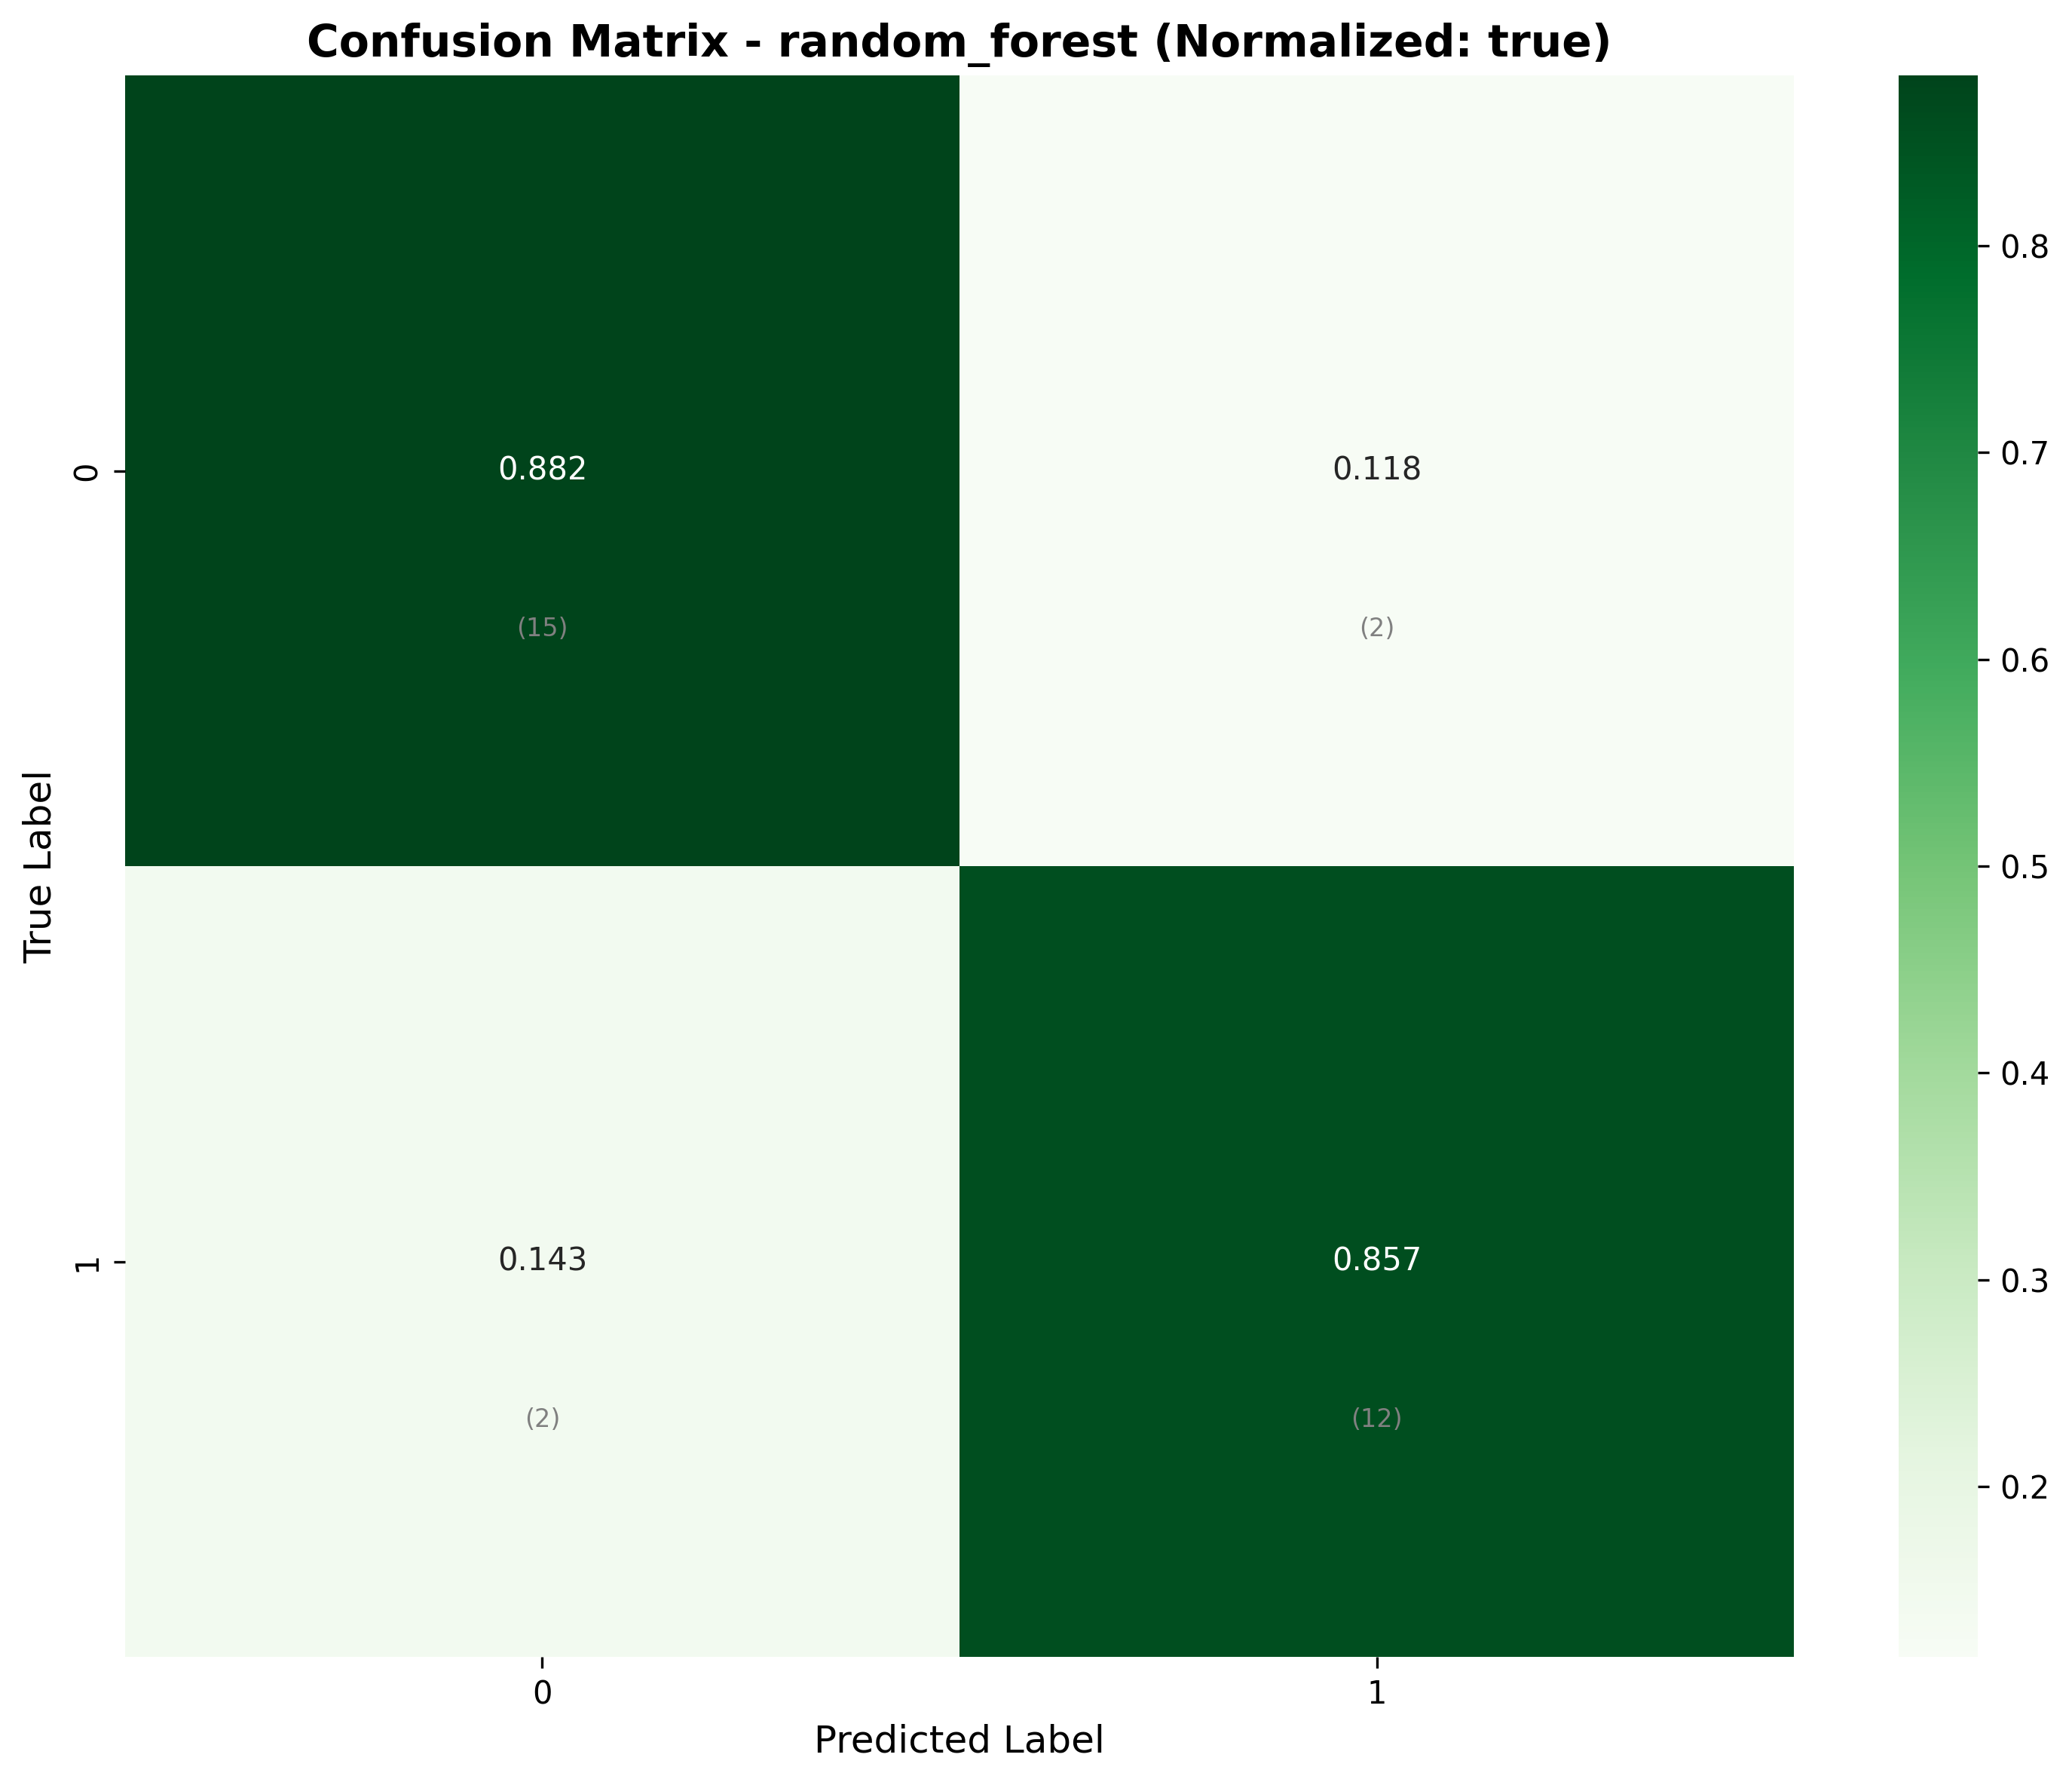
\includegraphics[width=0.95\textwidth]{Result/cleveland_dataset/confusion_matrices/random_forest_numeric_dataset_StandardScaler.png}
\caption{RF Cleveland (87.1\%)}
\label{fig:ra-rf_performance_standard}
\end{subfigure}
\hfill
\begin{subfigure}[b]{0.31\textwidth}
\centering
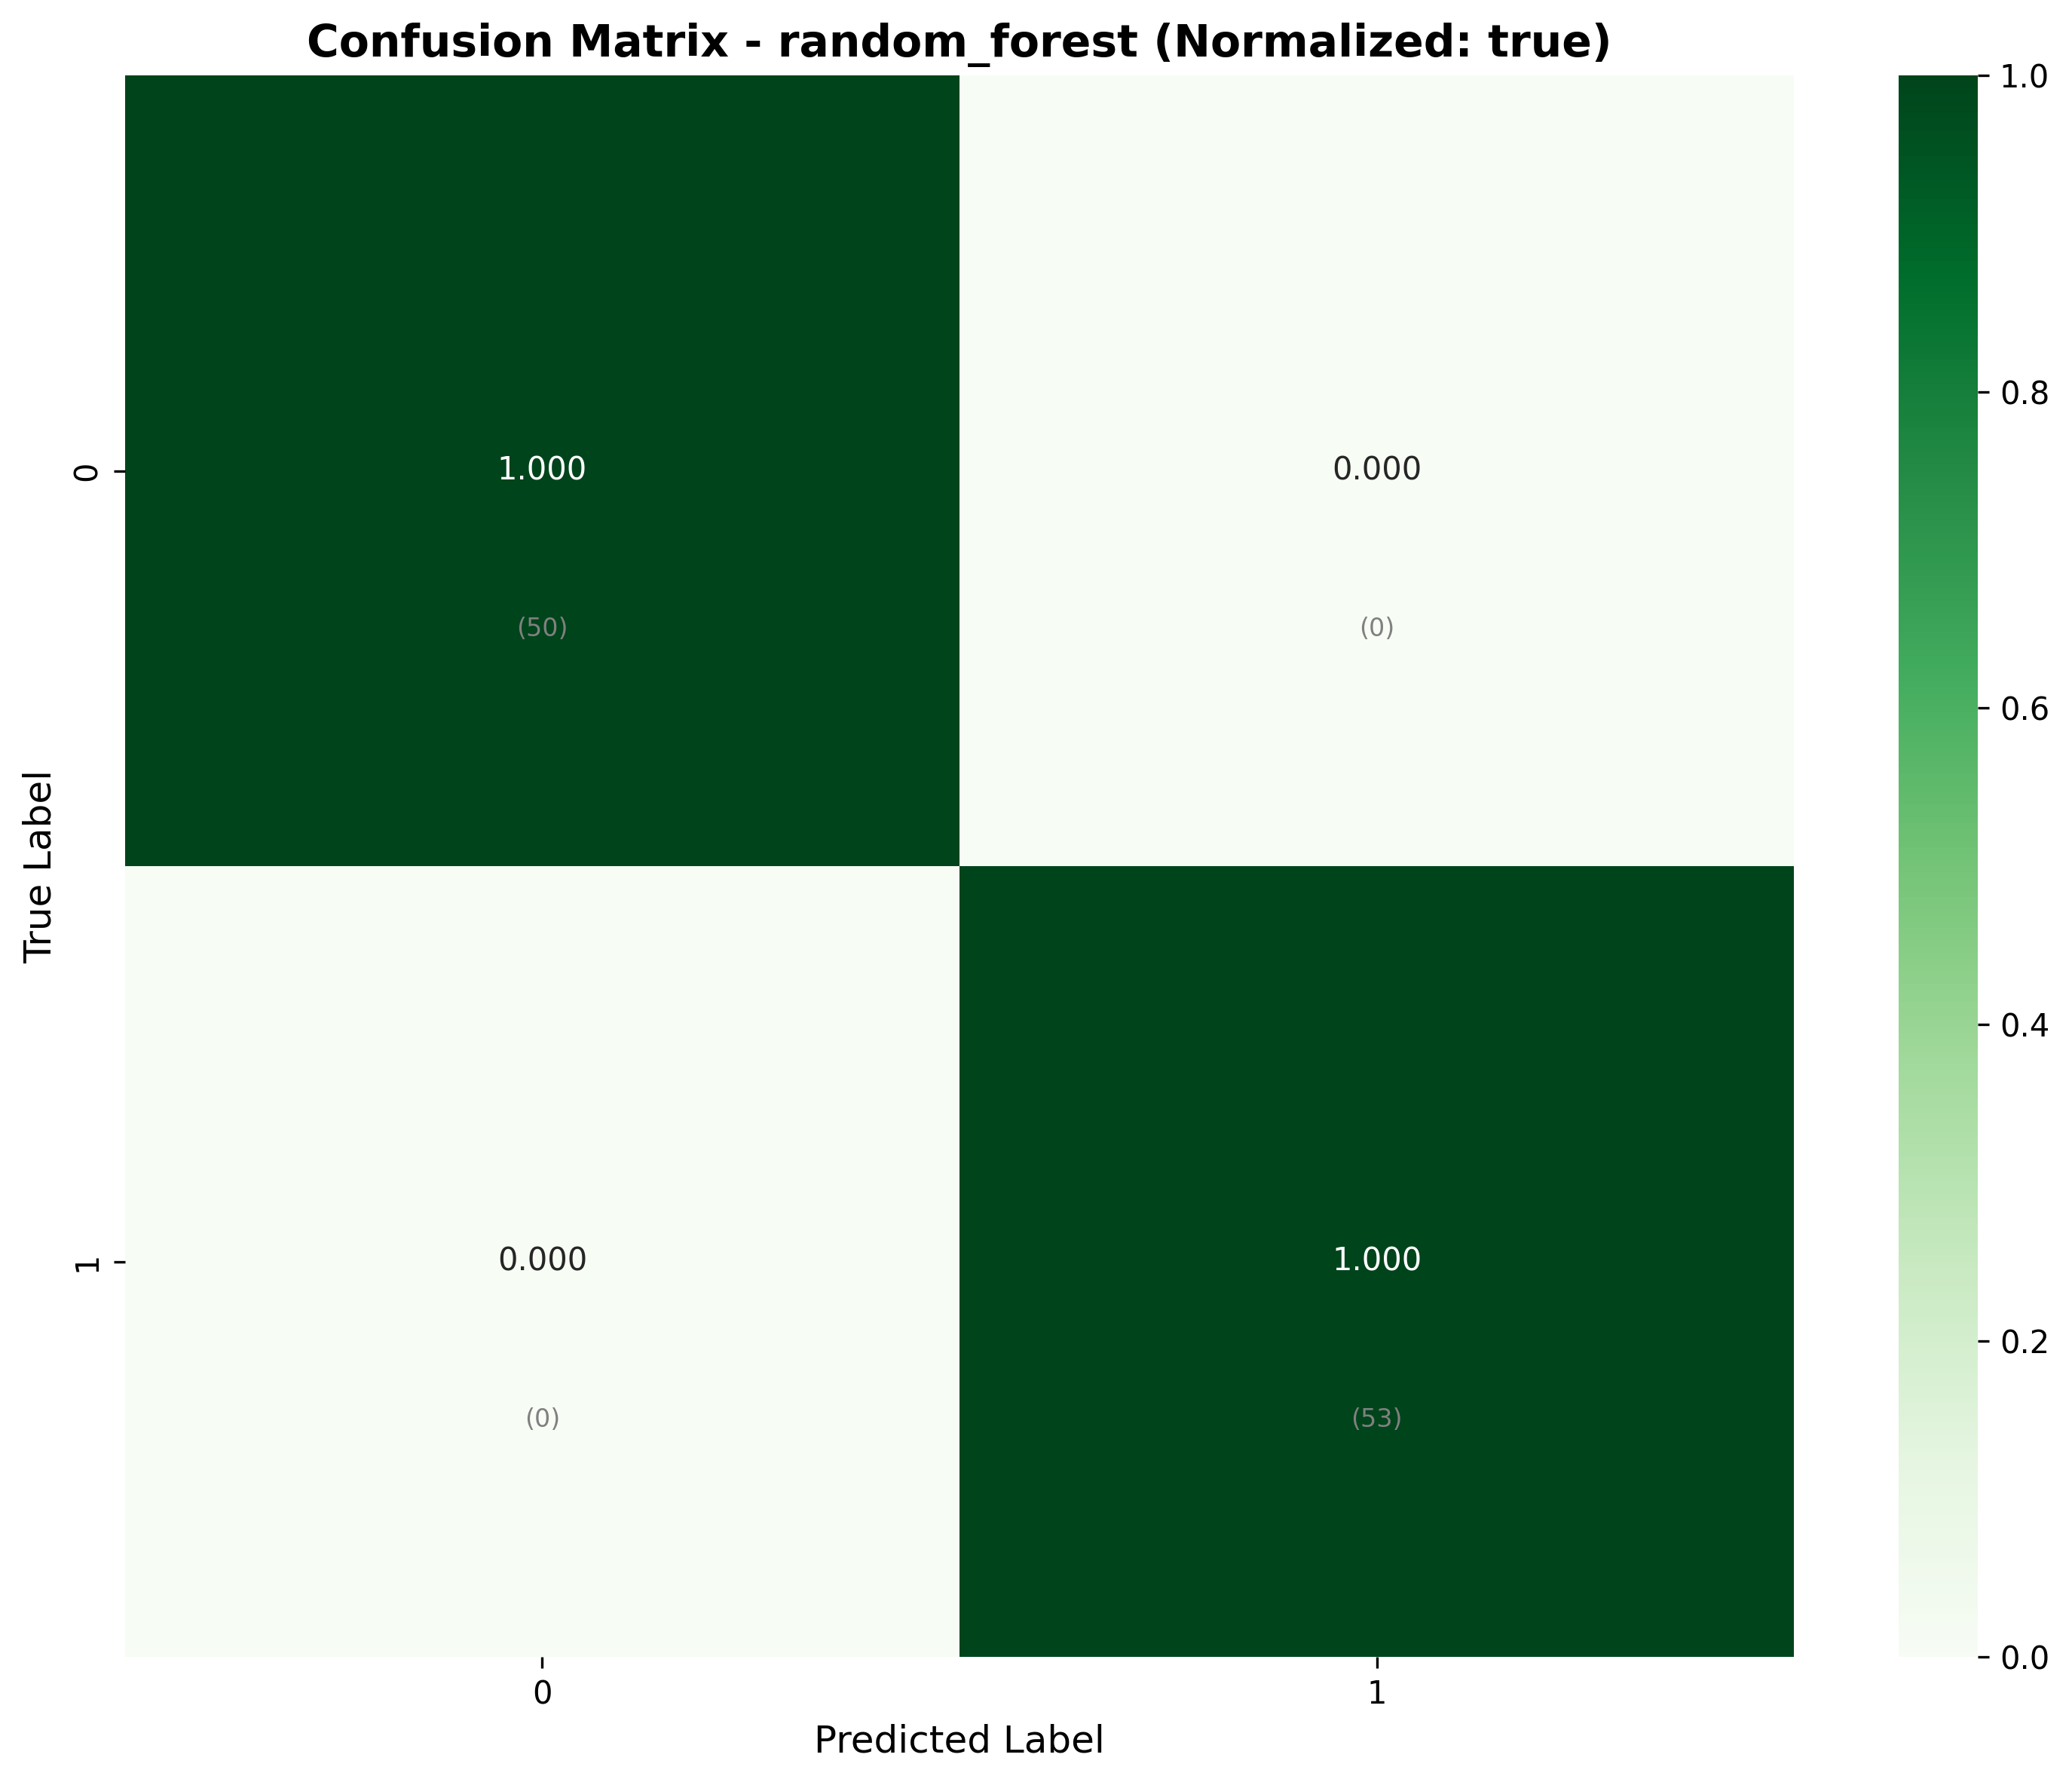
\includegraphics[width=0.95\textwidth]{Result/heart_dataset/confusion_matrices/random_forest_numeric_dataset_StandardScaler.png}
\caption{RF Heart (100\%)}
\label{fig:ra-rf_performance_heart}
\end{subfigure}
\hfill
\begin{subfigure}[b]{0.31\textwidth}
\centering
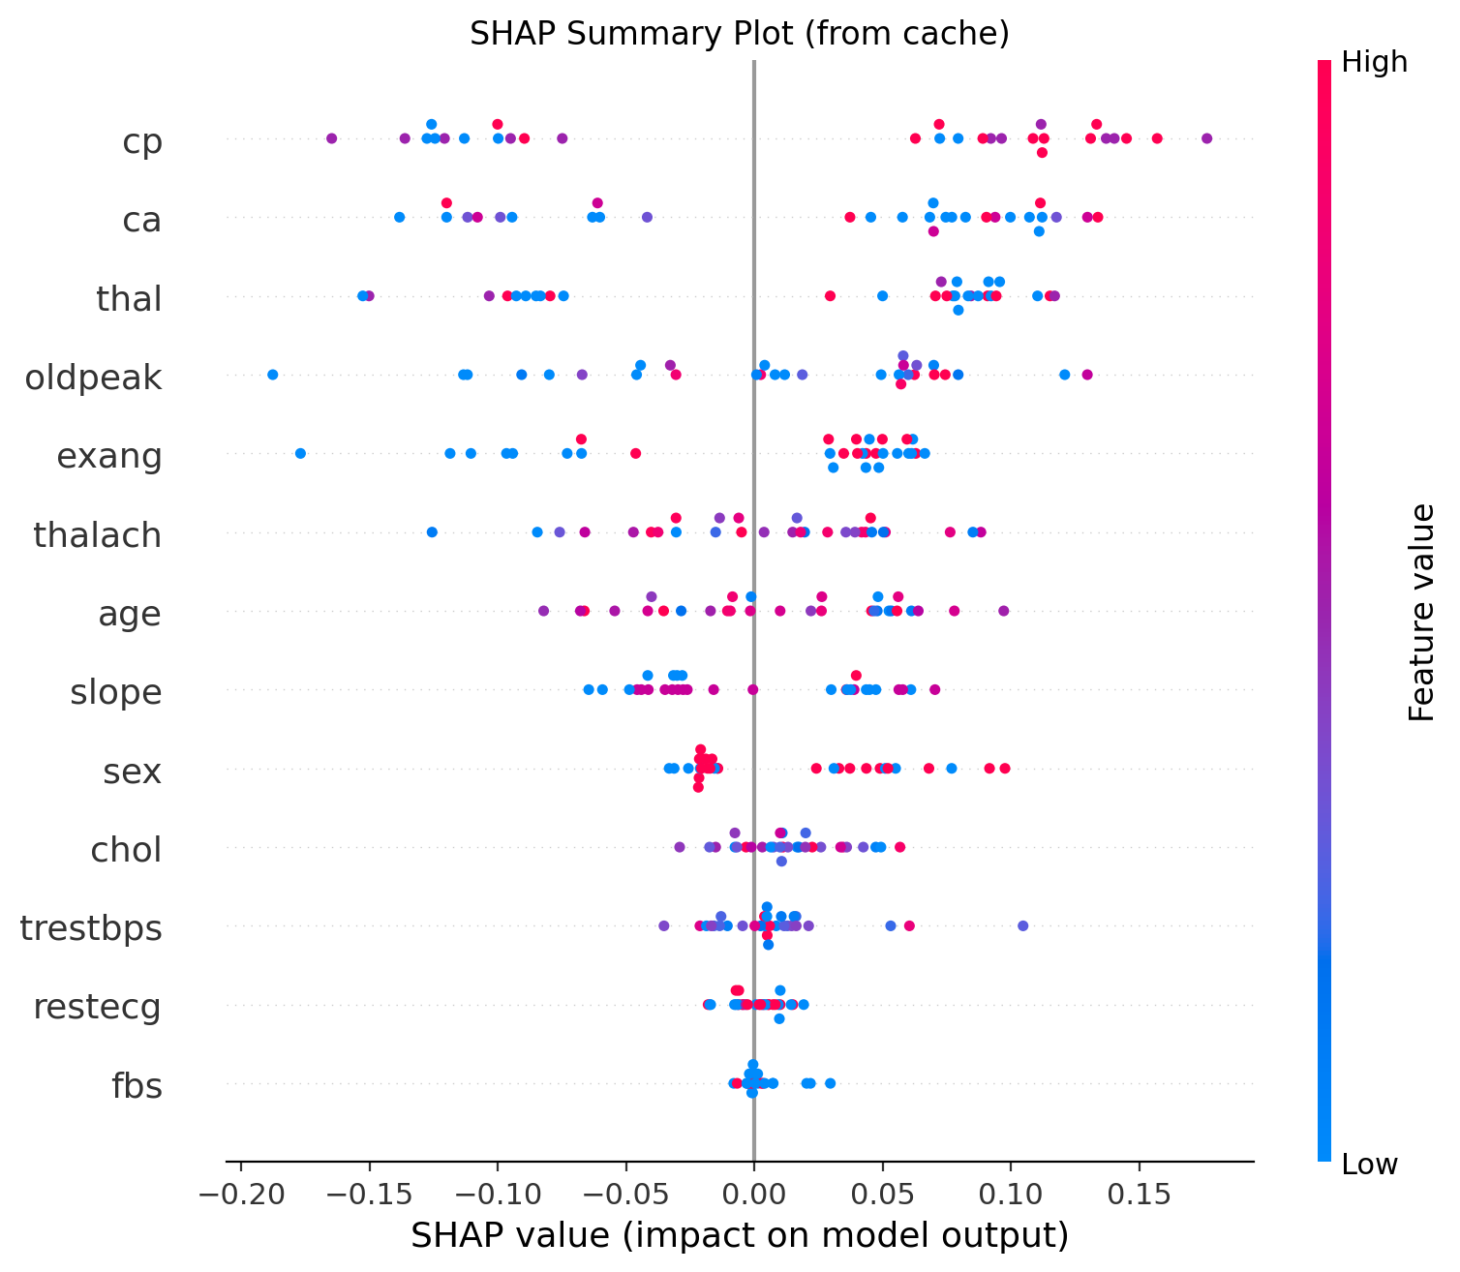
\includegraphics[width=0.95\textwidth]{Result/cleveland_dataset/RF/SHAP/Summary.png}
\caption{RF Feature Importance}
\label{fig:ra-rf_shap_summary}
\end{subfigure}
\caption{Random Forest Performance và Feature Importance: Cross-dataset comparison cho production readiness assessment}
\label{fig:ra-rf_cross_dataset}
\end{figure}

Hình \ref{fig:ra-rf_cross_dataset} chứng minh tính ổn định và hiệu suất mạnh mẽ của Random Forest với hệ thống phân cấp đặc trưng nhất quán qua các dataset.

\textbf{CatBoost}: Cleveland (93.5\% tối đa) → Heart (100\% across scalers). CatBoost vượt trội với xử lý đặc trưng phân loại tự động, đặc biệt với loại đau ngực (cp) và kết quả thallium (thal), phản ánh việc xử lý vượt trội các đặc trưng lâm sàng phân loại/thứ tự.

\begin{figure}[H]
\centering
\begin{subfigure}[b]{0.48\textwidth}
\centering
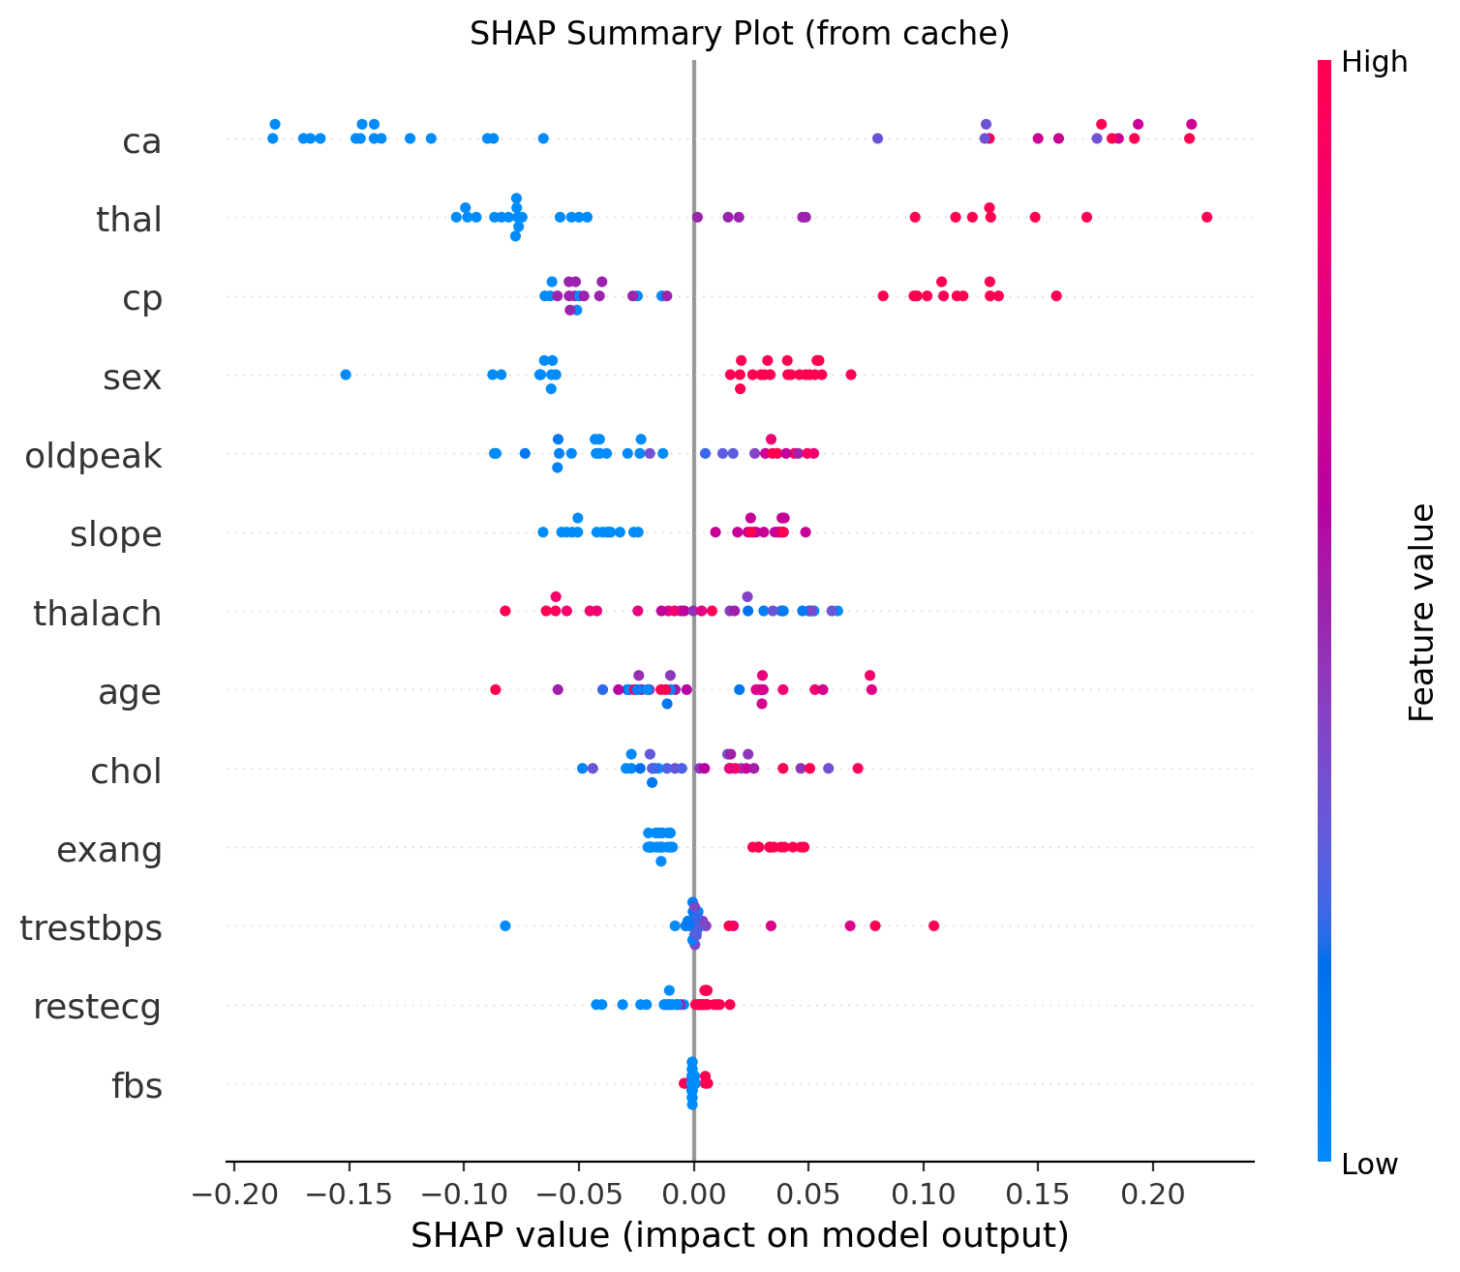
\includegraphics[width=0.95\textwidth]{Result/cleveland_dataset/Catboost/SHAP/Summary.png}
\caption{CatBoost Cleveland Feature Importance}
\label{fig:catboost_shap_cleveland}
\end{subfigure}
\hfill
\begin{subfigure}[b]{0.48\textwidth}
\centering
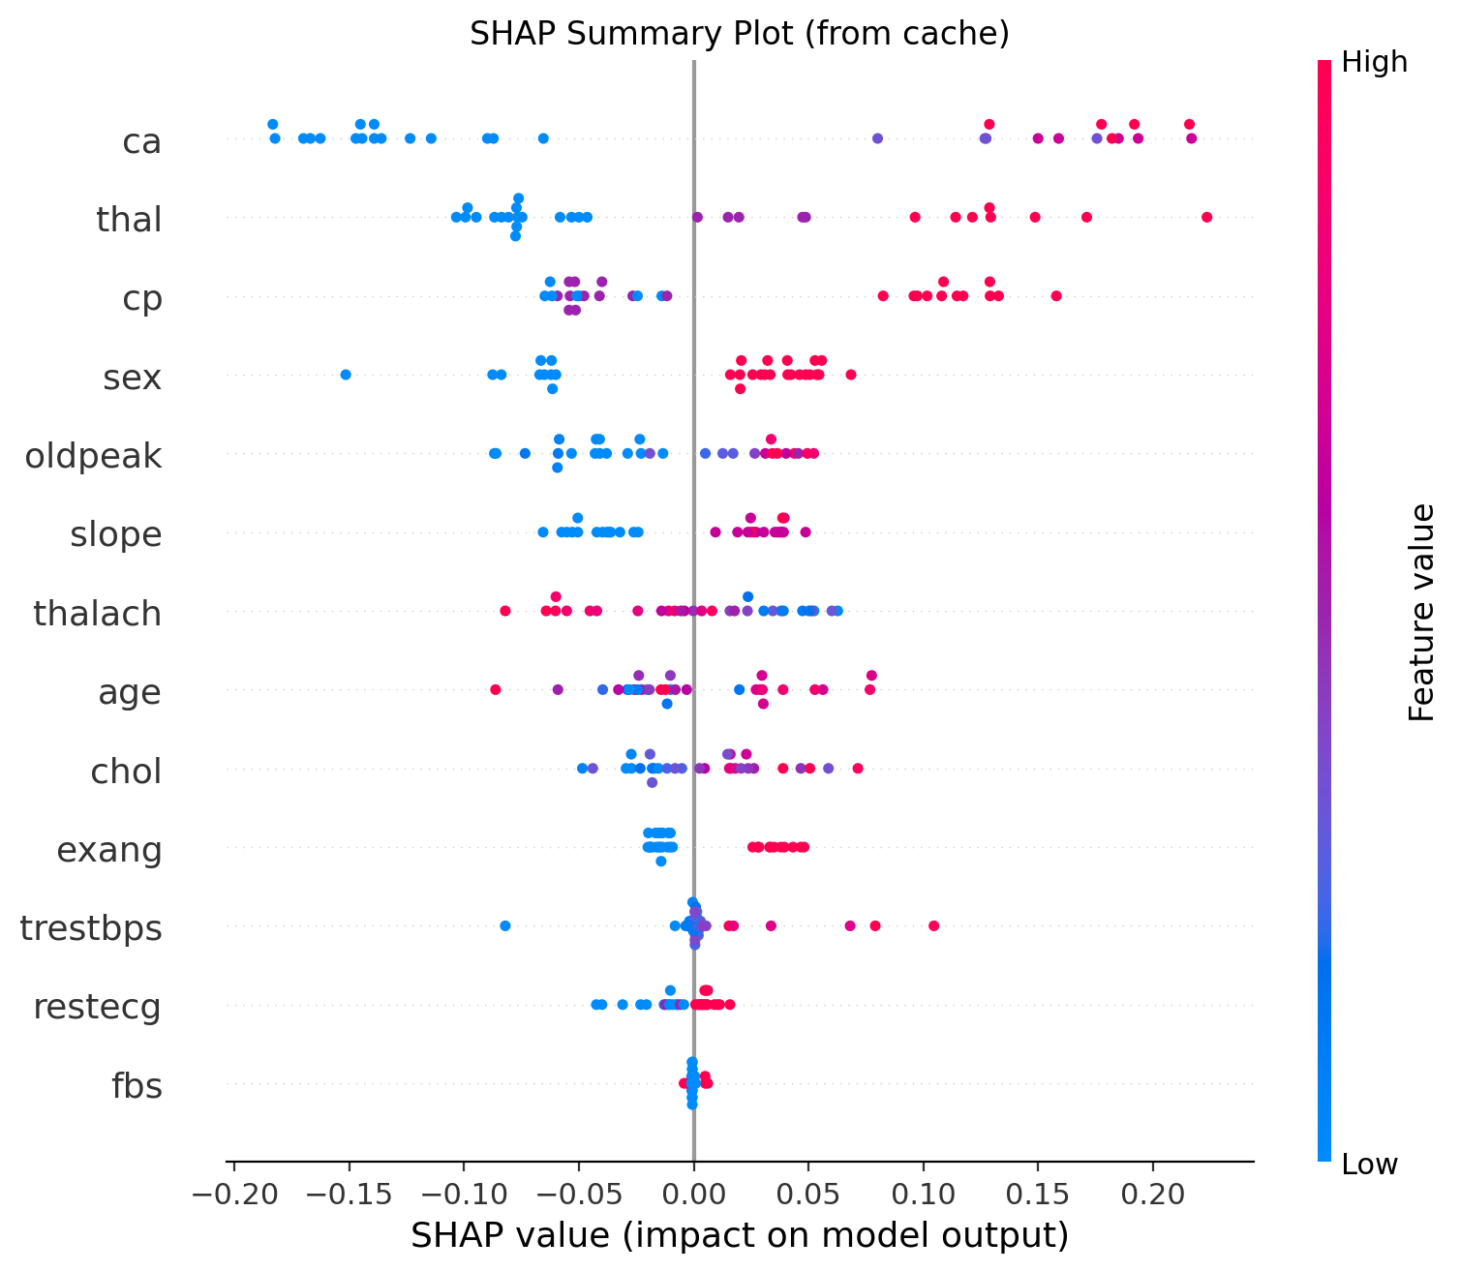
\includegraphics[width=0.95\textwidth]{Result/heart_dataset/Catboost/SHAP/Summary.png}
\caption{CatBoost Heart Feature Importance}
\label{fig:catboost_shap_heart}
\end{subfigure}
\caption{CatBoost SHAP Analysis: Superior categorical feature handling với consistent cp và thal dominance}
\label{fig:ra-catboost_shap_comparison}
\end{figure}

Figure \ref{fig:ra-catboost_shap_comparison} illustrates CatBoost's automatic categorical encoding advantage với chest pain type (cp) và thallium results (thal) maintaining top importance across datasets.

\textbf{XGBoost}: Cleveland (87.1\%) → Heart (95-100\%). Efficient gradient boosting với good regularization cho large datasets, với strong feature hierarchies consistent across scalers.

\begin{figure}[H]
\centering
\begin{subfigure}[b]{0.48\textwidth}
\centering
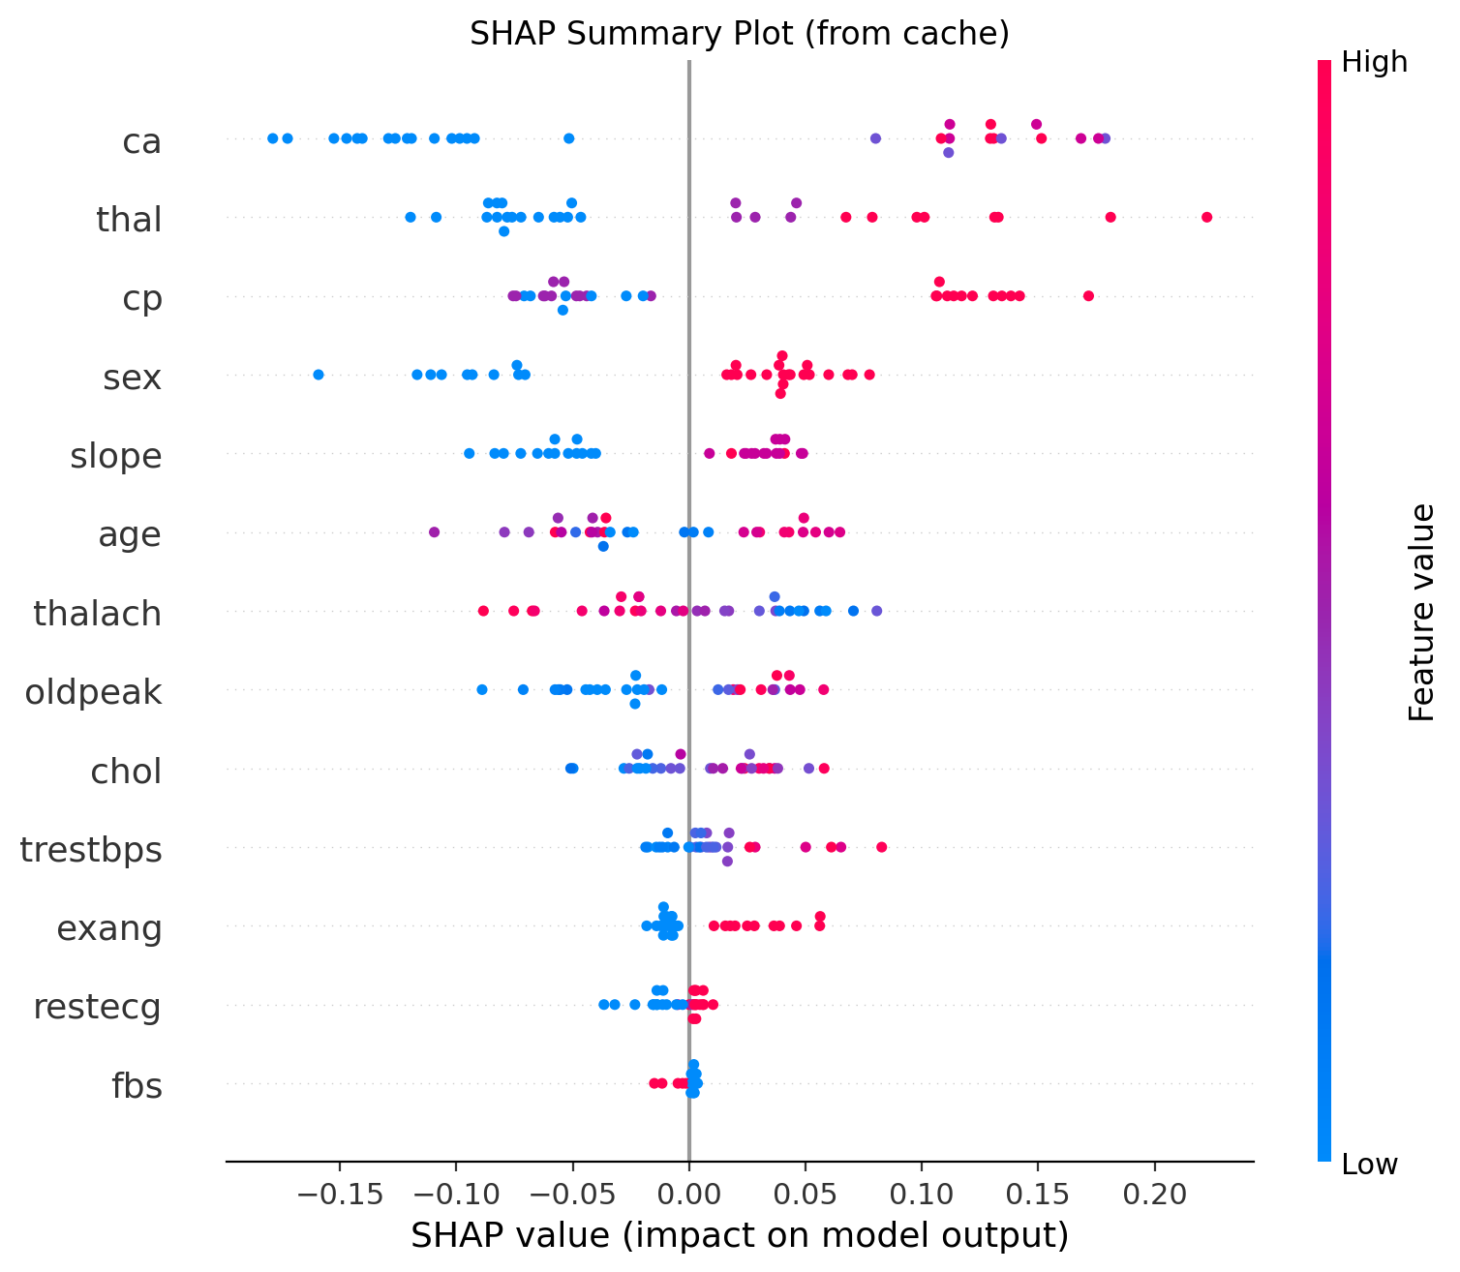
\includegraphics[width=0.95\textwidth]{Result/cleveland_dataset/XGBoost/SHAP/Summary.png}
\caption{XGBoost Cleveland - Feature Importance}
\label{fig:xgboost_shap_cleveland_analysis}
\end{subfigure}
\hfill
\begin{subfigure}[b]{0.48\textwidth}
\centering
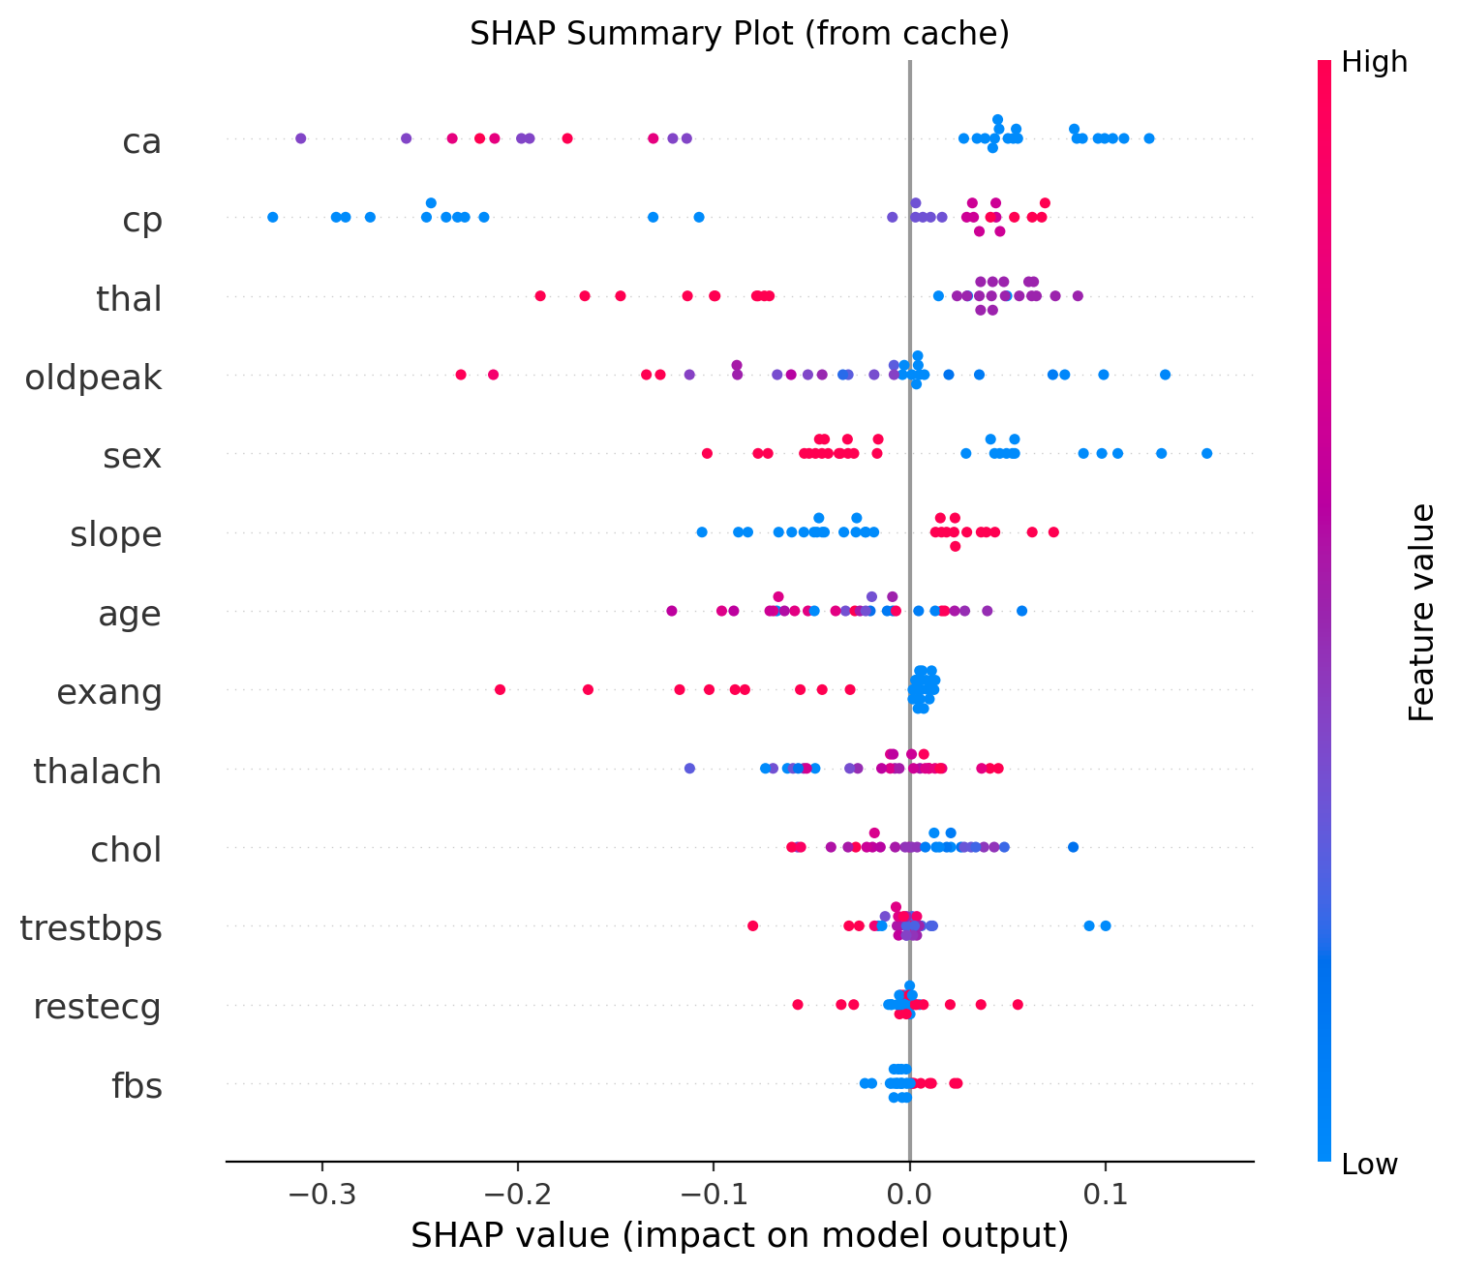
\includegraphics[width=0.95\textwidth]{Result/heart_dataset/XGBoost/SHAP/Summary.png}
\caption{XGBoost Heart - Feature Importance}
\label{fig:xgboost_shap_heart_analysis}
\end{subfigure}
\caption{XGBoost Cross-Dataset Analysis: Strong regularization và feature hierarchy consistency}
\label{fig:xgboost_analysis_complete}
\end{figure}

\textbf{LightGBM}: Cleveland (80.6\%) → Heart (100\%). Memory-efficient gradient boosting với fast training times (3.3-3.6 seconds), scalable cho các ứng dụng lâm sàng yêu cầu triển khai mô hình nhanh.

\begin{figure}[H]
\centering
\begin{subfigure}[b]{0.48\textwidth}
\centering
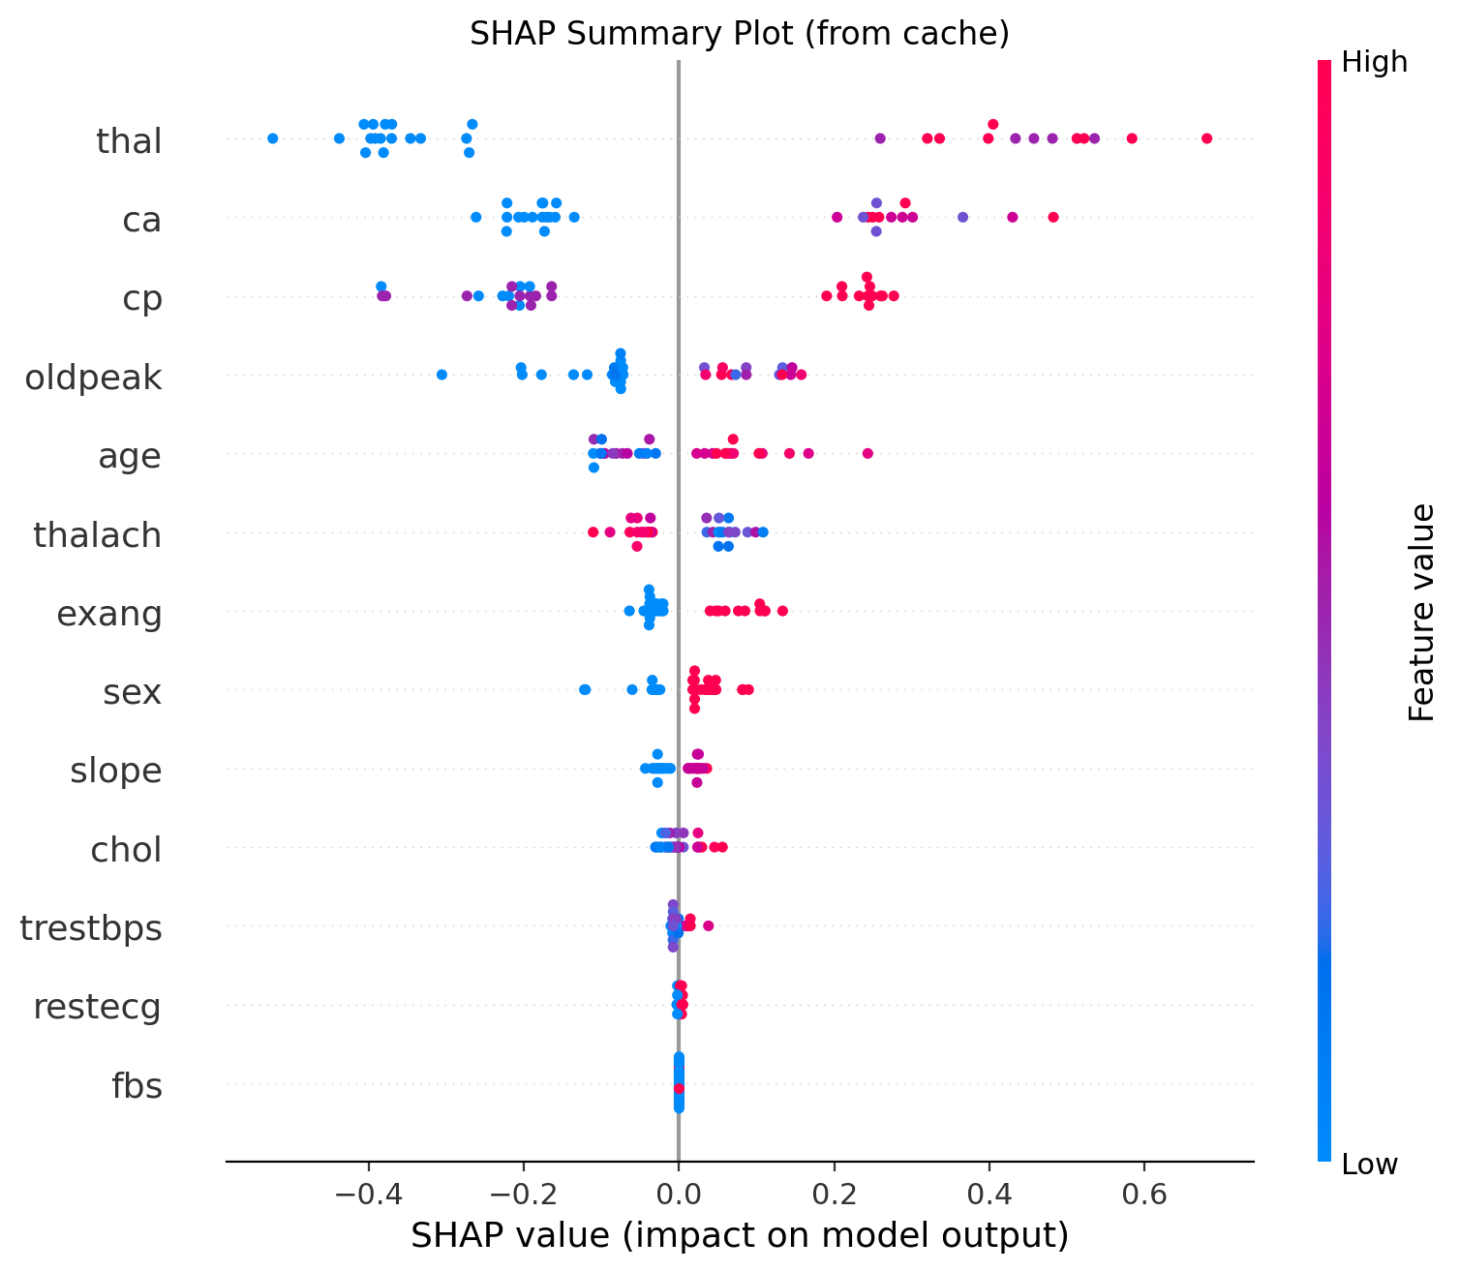
\includegraphics[width=0.95\textwidth]{Result/cleveland_dataset/LightGBM/SHAP/Summary.png}
\caption{LightGBM Cleveland Feature Importance}
\label{fig:lightgbm_shap_cleveland_analysis}
\end{subfigure}
\hfill
\begin{subfigure}[b]{0.48\textwidth}
\centering
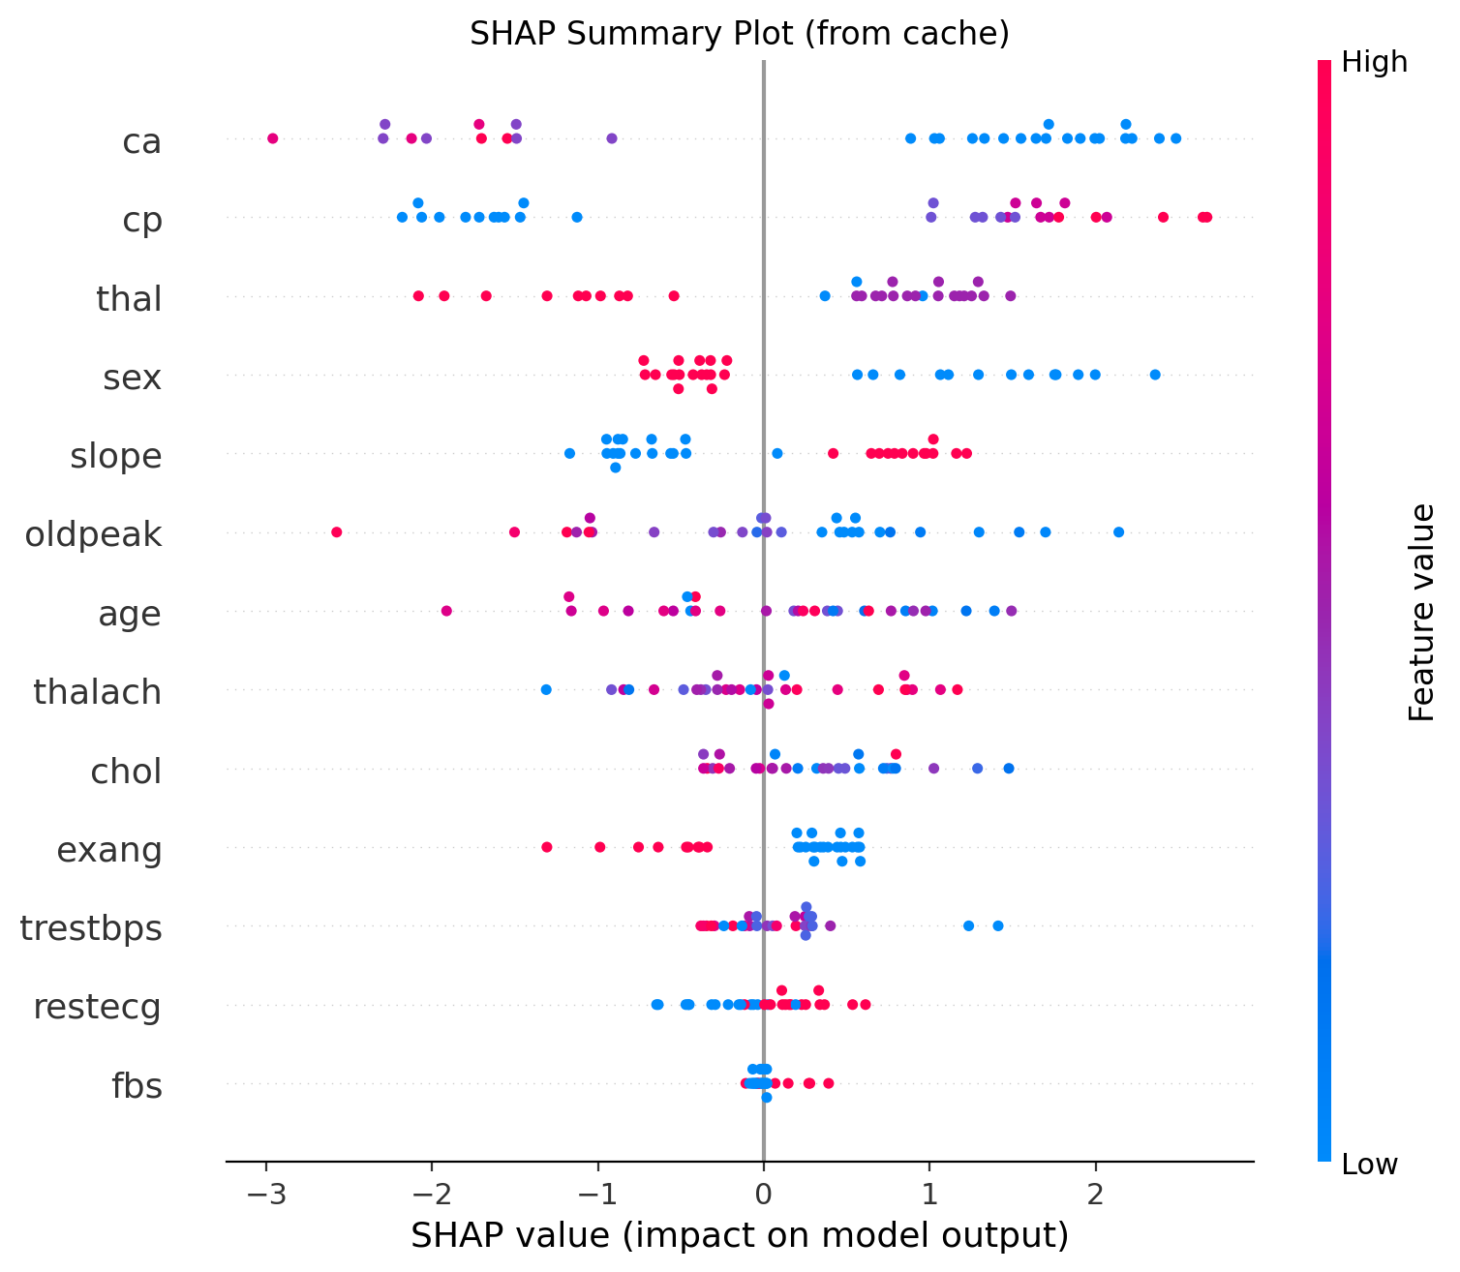
\includegraphics[width=0.95\textwidth]{Result/heart_dataset/LightGBM/SHAP/Summary.png}
\caption{LightGBM Heart Feature Importance}
\label{fig:lightgbm_shap_heart_analysis}
\end{subfigure}
\caption{LightGBM Efficiency Analysis: Fast training với strong performance scaling}
\label{fig:lightgbm_analysis_complete}
\end{figure}

Figures \ref{fig:xgboost_analysis_complete} và \ref{fig:lightgbm_analysis_complete} demonstrate different approaches của gradient boosting family với consistent clinical predictors hierarchy across datasets.

\textbf{Decision Tree}: Cleveland (74.2-80.6\%) → Heart (variable performance). Single tree approach với direct interpretability advantages, useful cho clinical decision rules extraction và patient stratification protocol development.

\begin{figure}[H]
\centering
\begin{subfigure}[b]{0.48\textwidth}
\centering
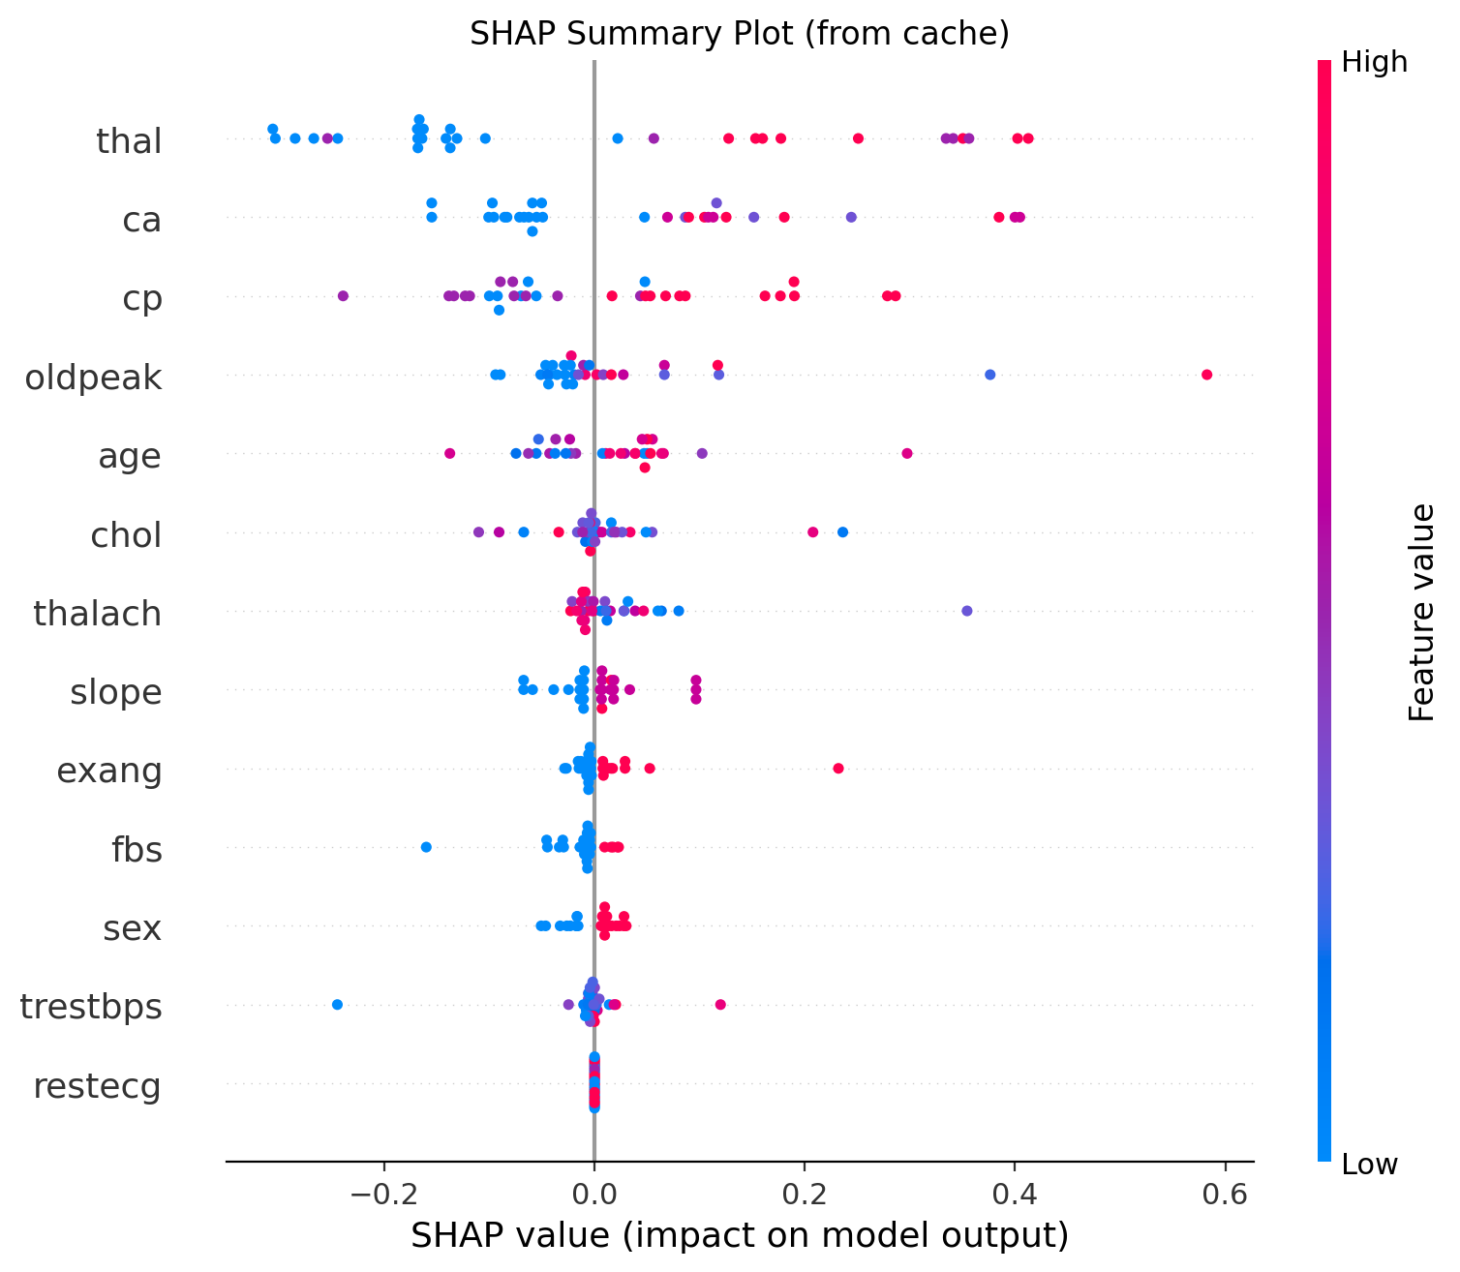
\includegraphics[width=0.95\textwidth]{Result/cleveland_dataset/DT/SHAP/Summary.png}
\caption{Decision Tree Cleveland Feature Importance}
\label{fig:dt_shap_cleveland_analysis}
\end{subfigure}
\hfill
\begin{subfigure}[b]{0.48\textwidth}
\centering
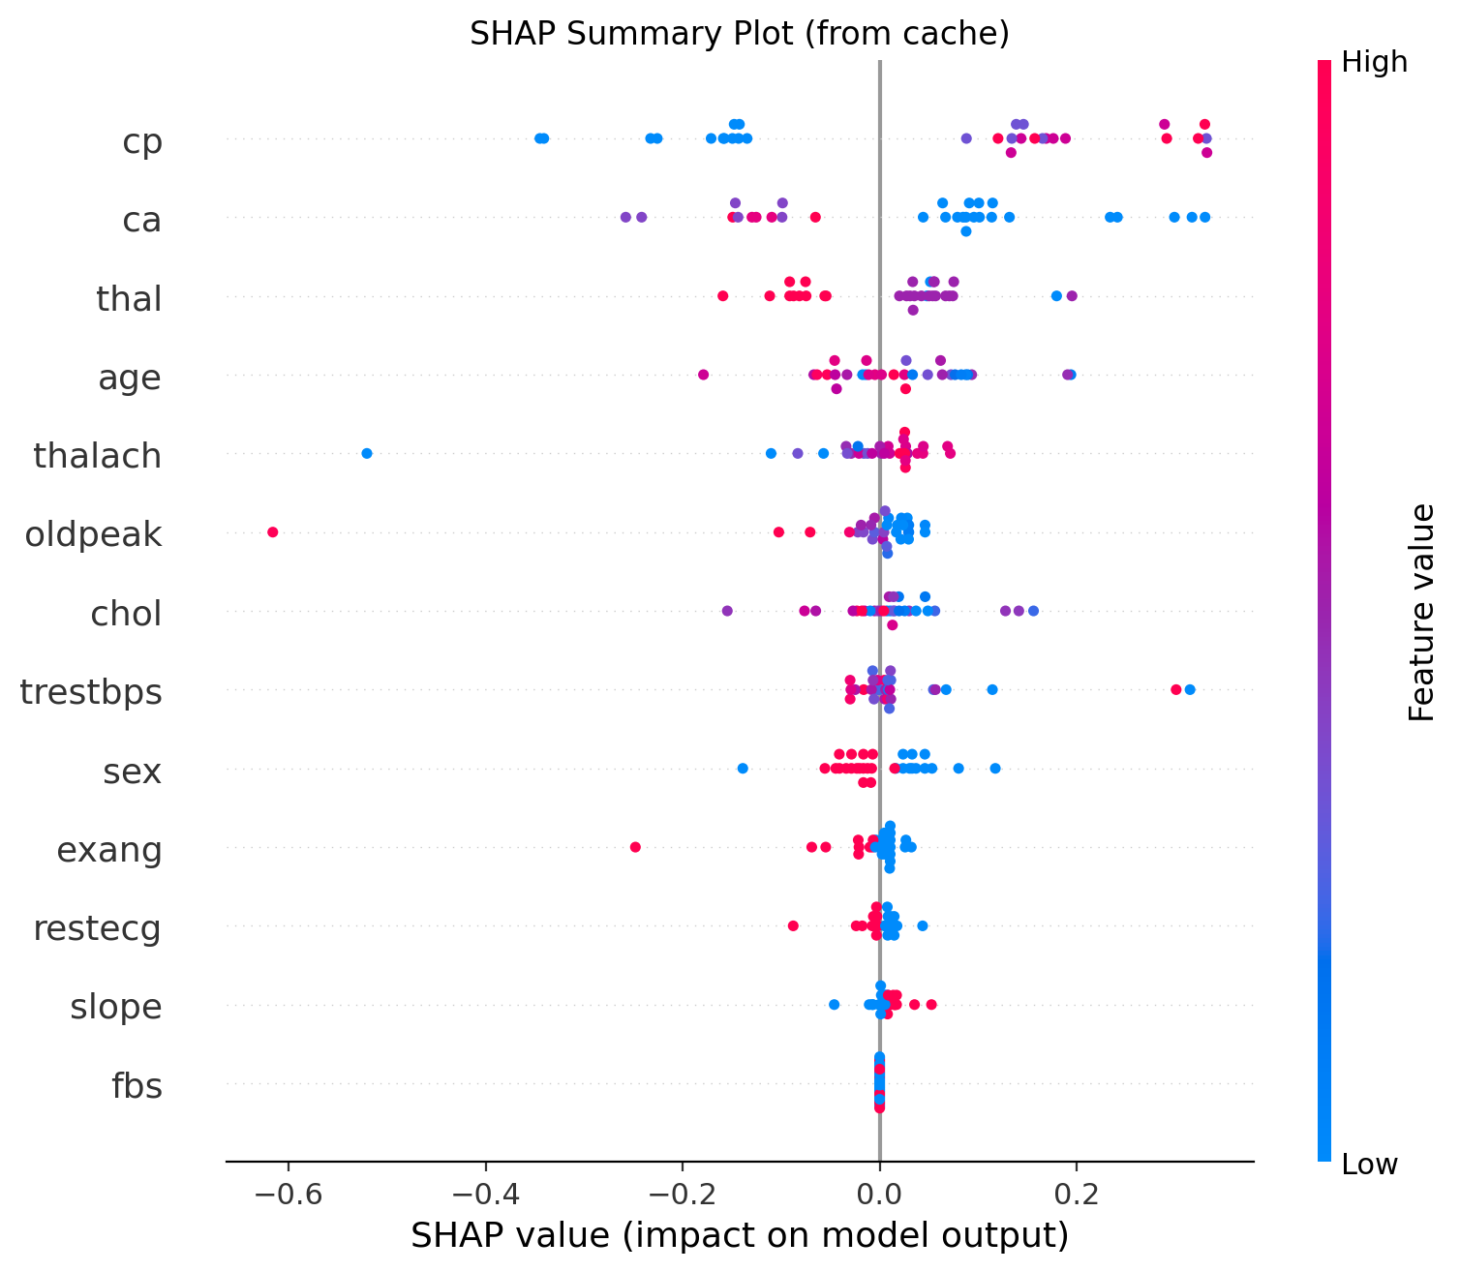
\includegraphics[width=0.95\textwidth]{Result/heart_dataset/DT/SHAP/Summary.png}
\caption{Decision Tree Heart Feature Importance}
\label{fig:dt_shap_heart_analysis}
\end{subfigure}
\caption{Tính Giải thích Decision Tree: Quy tắc ra quyết định lâm sàng trực tiếp với tầm quan trọng đặc trưng minh bạch}
\label{fig:decision_tree_complete}
\end{figure}

\textbf{Gradient Boosting}: Cleveland (80.6-93.5\%) → Heart (hiệu suất mạnh). Gradient boosting cổ điển với tối ưu hóa tích cực và sửa lỗi tuần tự để cải thiện độ chính xác so với các cây đơn lẻ.

\begin{figure}[H]
\centering
\begin{subfigure}[b]{0.48\textwidth}
\centering
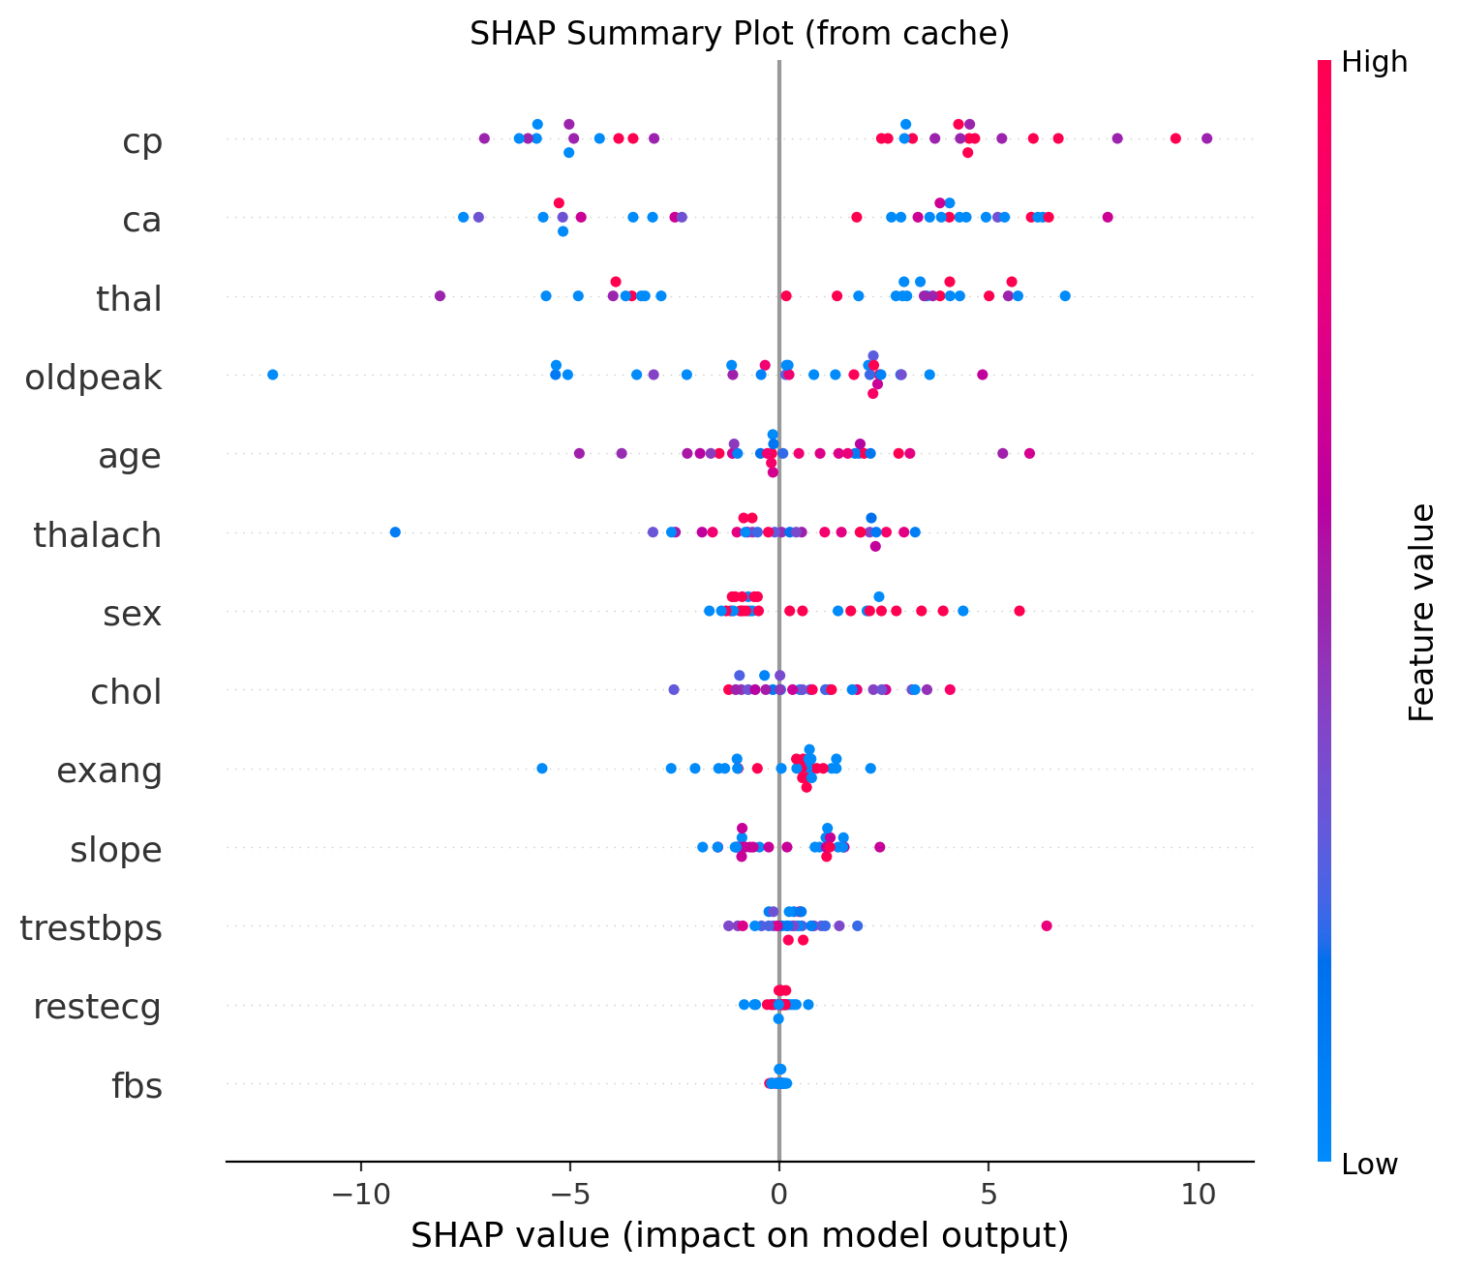
\includegraphics[width=0.95\textwidth]{Result/cleveland_dataset/GB/SHAP/Summary.png}
\caption{Gradient Boosting Cleveland Feature Importance}
\label{fig:gb_shap_cleveland_analysis}
\end{subfigure}
\hfill
\begin{subfigure}[b]{0.48\textwidth}
\centering
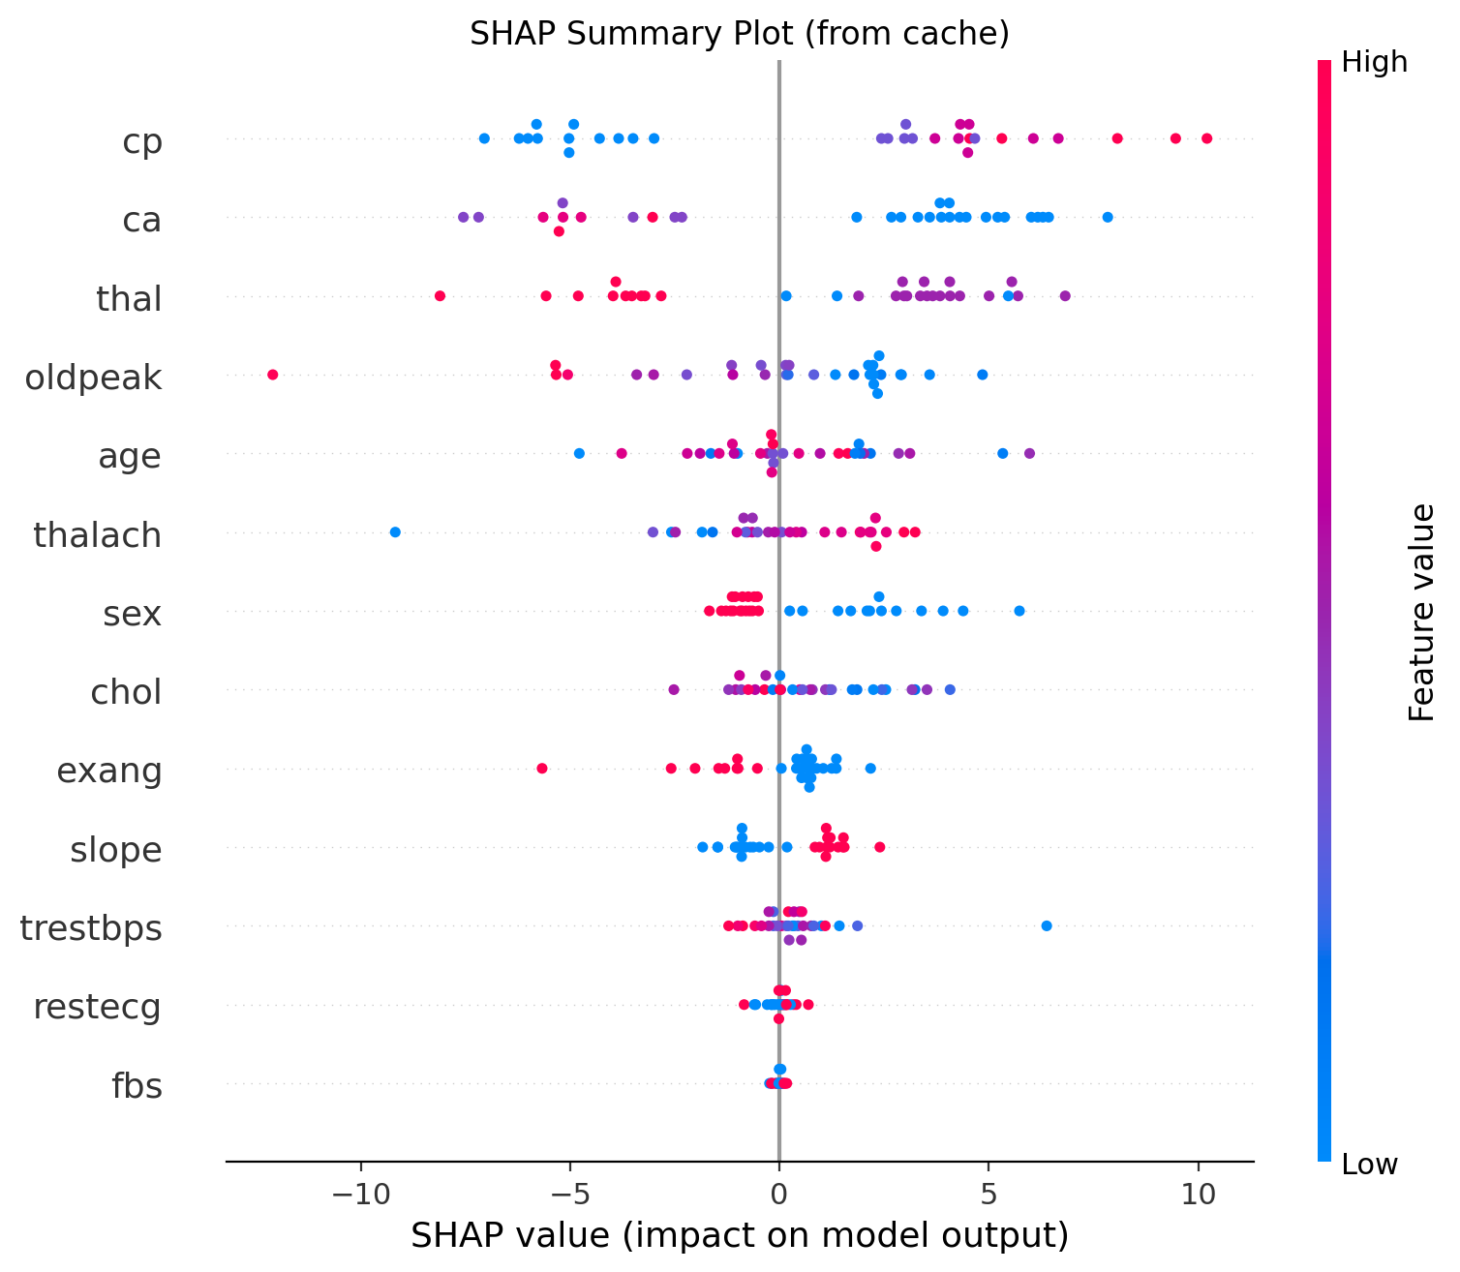
\includegraphics[width=0.95\textwidth]{Result/heart_dataset/GB/SHAP/Summary.png}
\caption{Gradient Boosting Heart Feature Importance}
\label{fig:gb_shap_heart_analysis}
\end{subfigure}
\caption{Gradient Boosting Sequential Learning: Advanced ensemble building với strong feature utilization}
\label{fig:gradient_boosting_complete}
\end{figure}

\paragraph{Classical Machine Learning Models}

\textbf{Logistic Regression}: Cleveland (80.6\%) → Heart (improved performance). Linear coefficients tương ứng với medical odds ratios, excellent baseline cho comparison với extremely fast training (0.04-0.05 seconds), computationally efficient cho real-time clinical decision support.

\begin{figure}[H]
\centering
\begin{subfigure}[b]{0.31\textwidth}
\centering
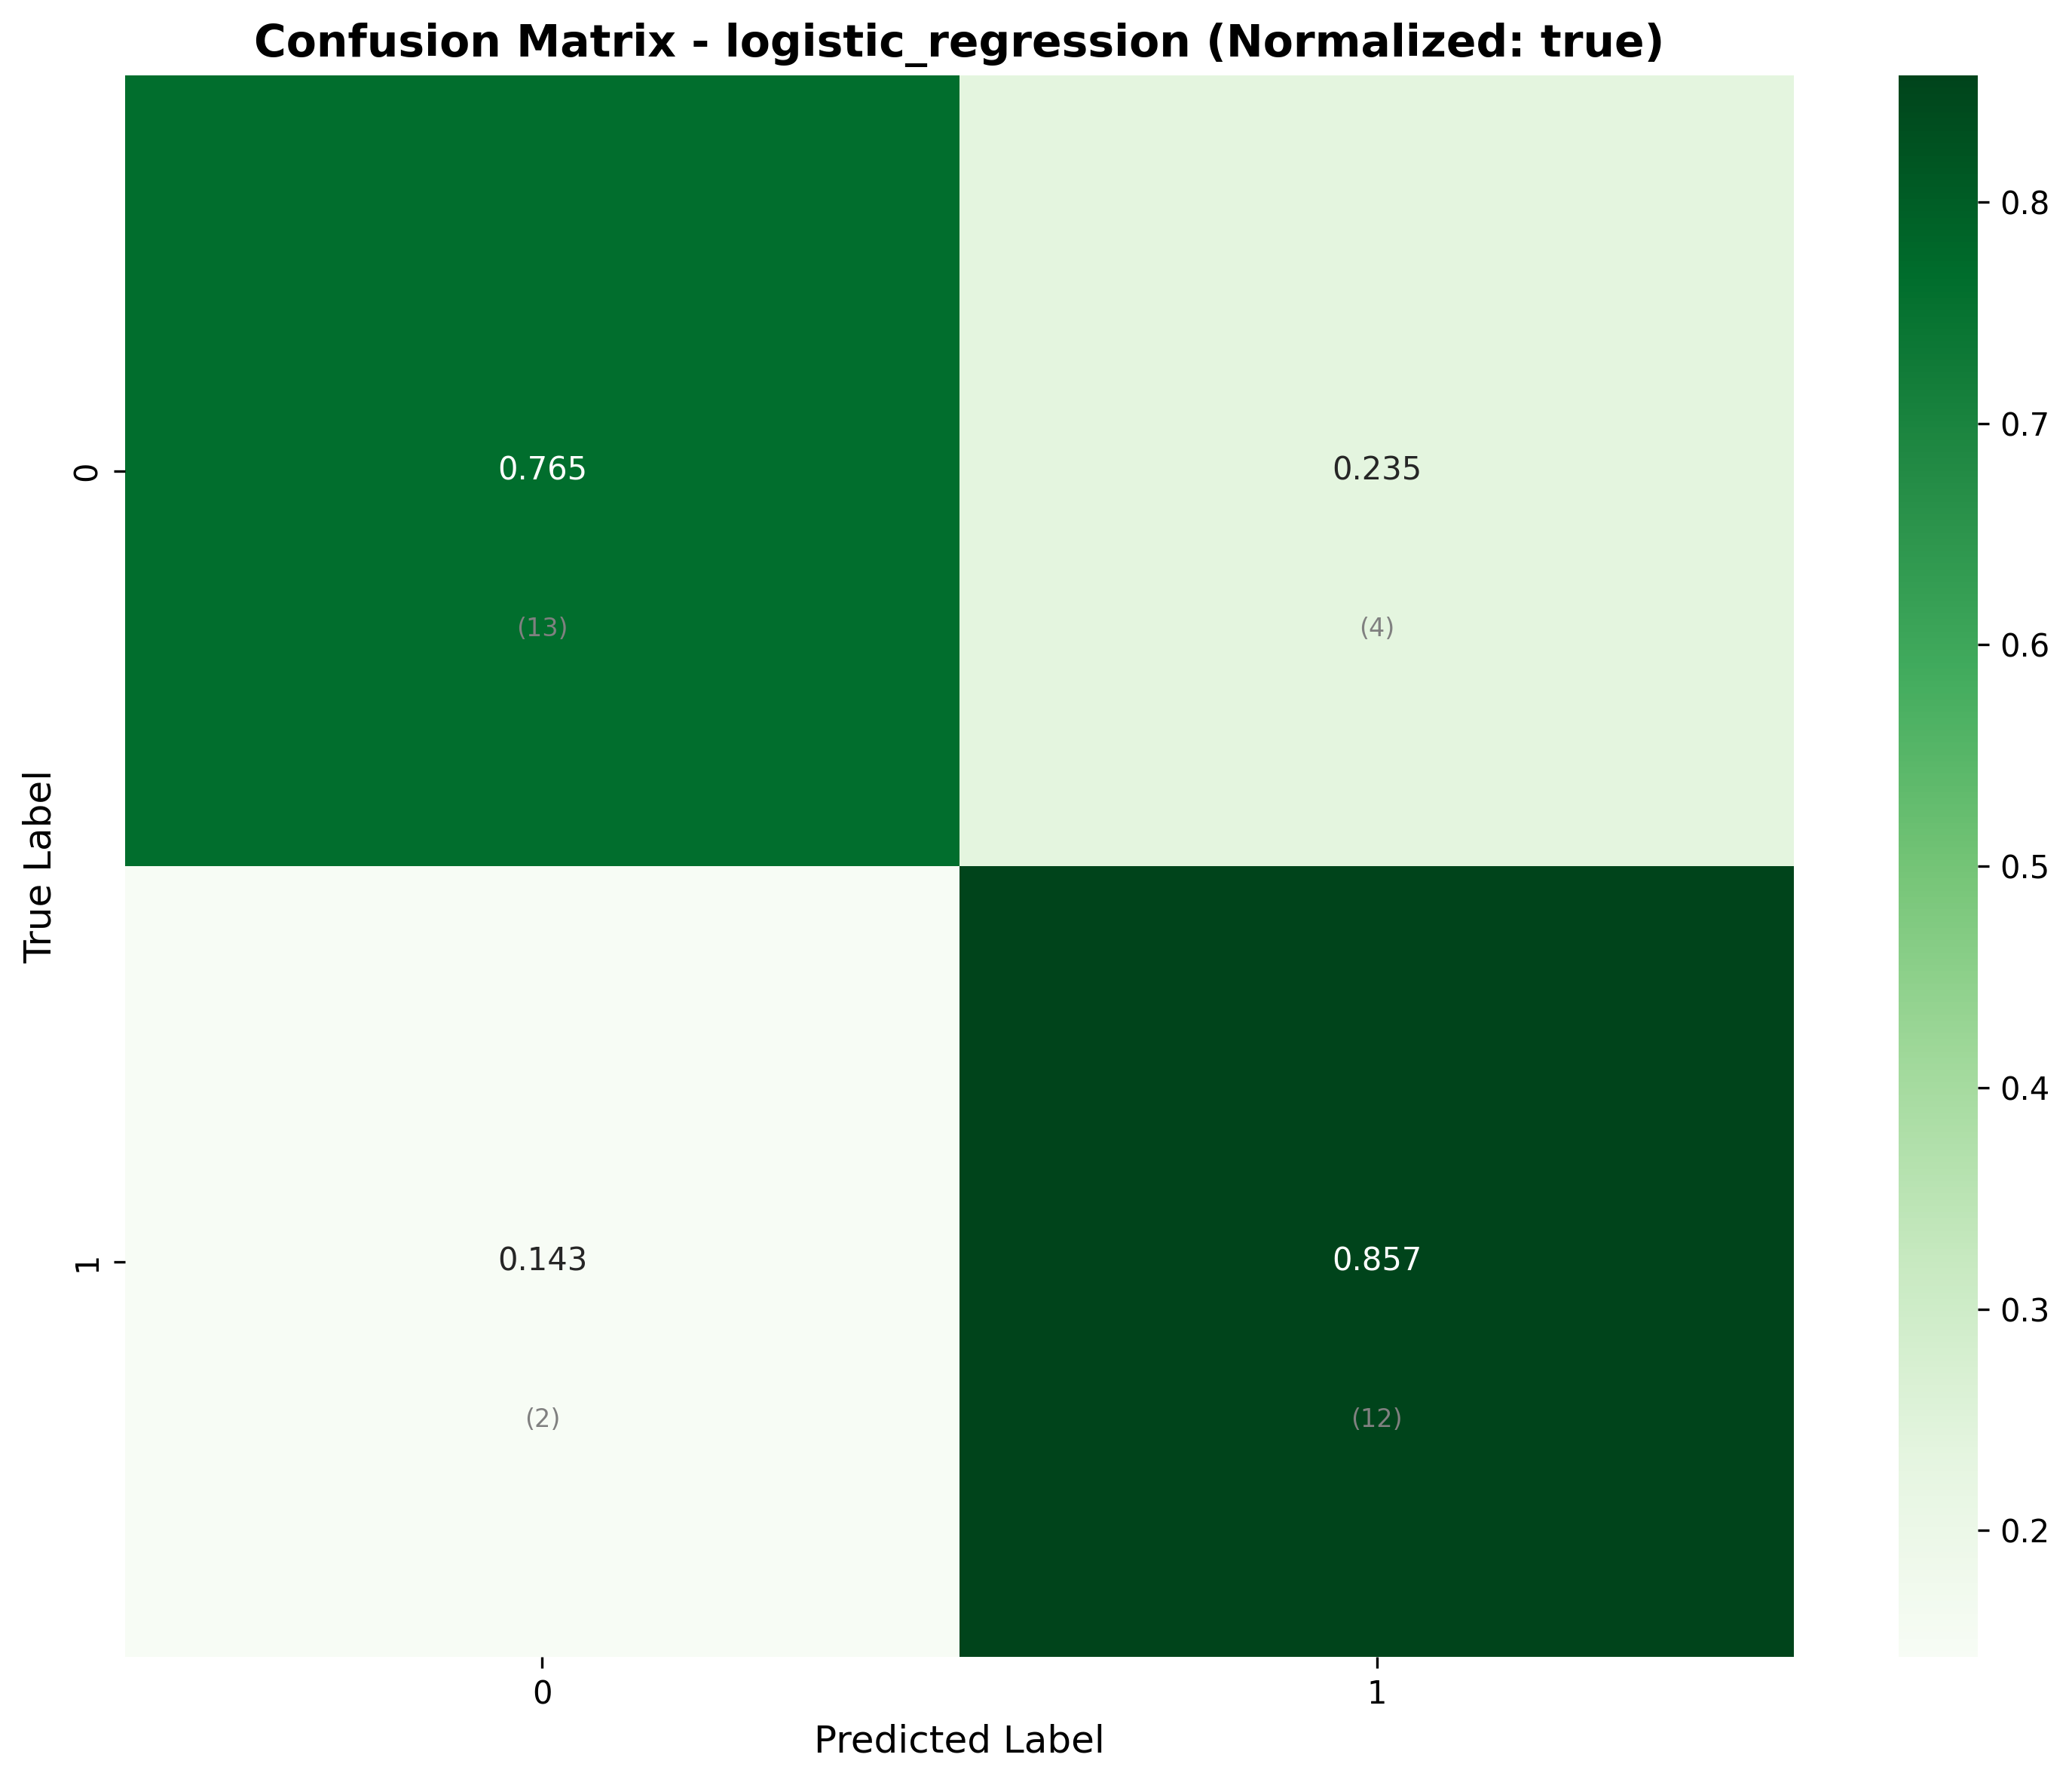
\includegraphics[width=0.95\textwidth]{Result/cleveland_dataset/confusion_matrices/logistic_regression_numeric_dataset_StandardScaler.png}
\caption{LR Cleveland (80.6\%)}
\label{fig:lr_cleveland_confusion}
\end{subfigure}
\hfill
\begin{subfigure}[b]{0.31\textwidth}
\centering
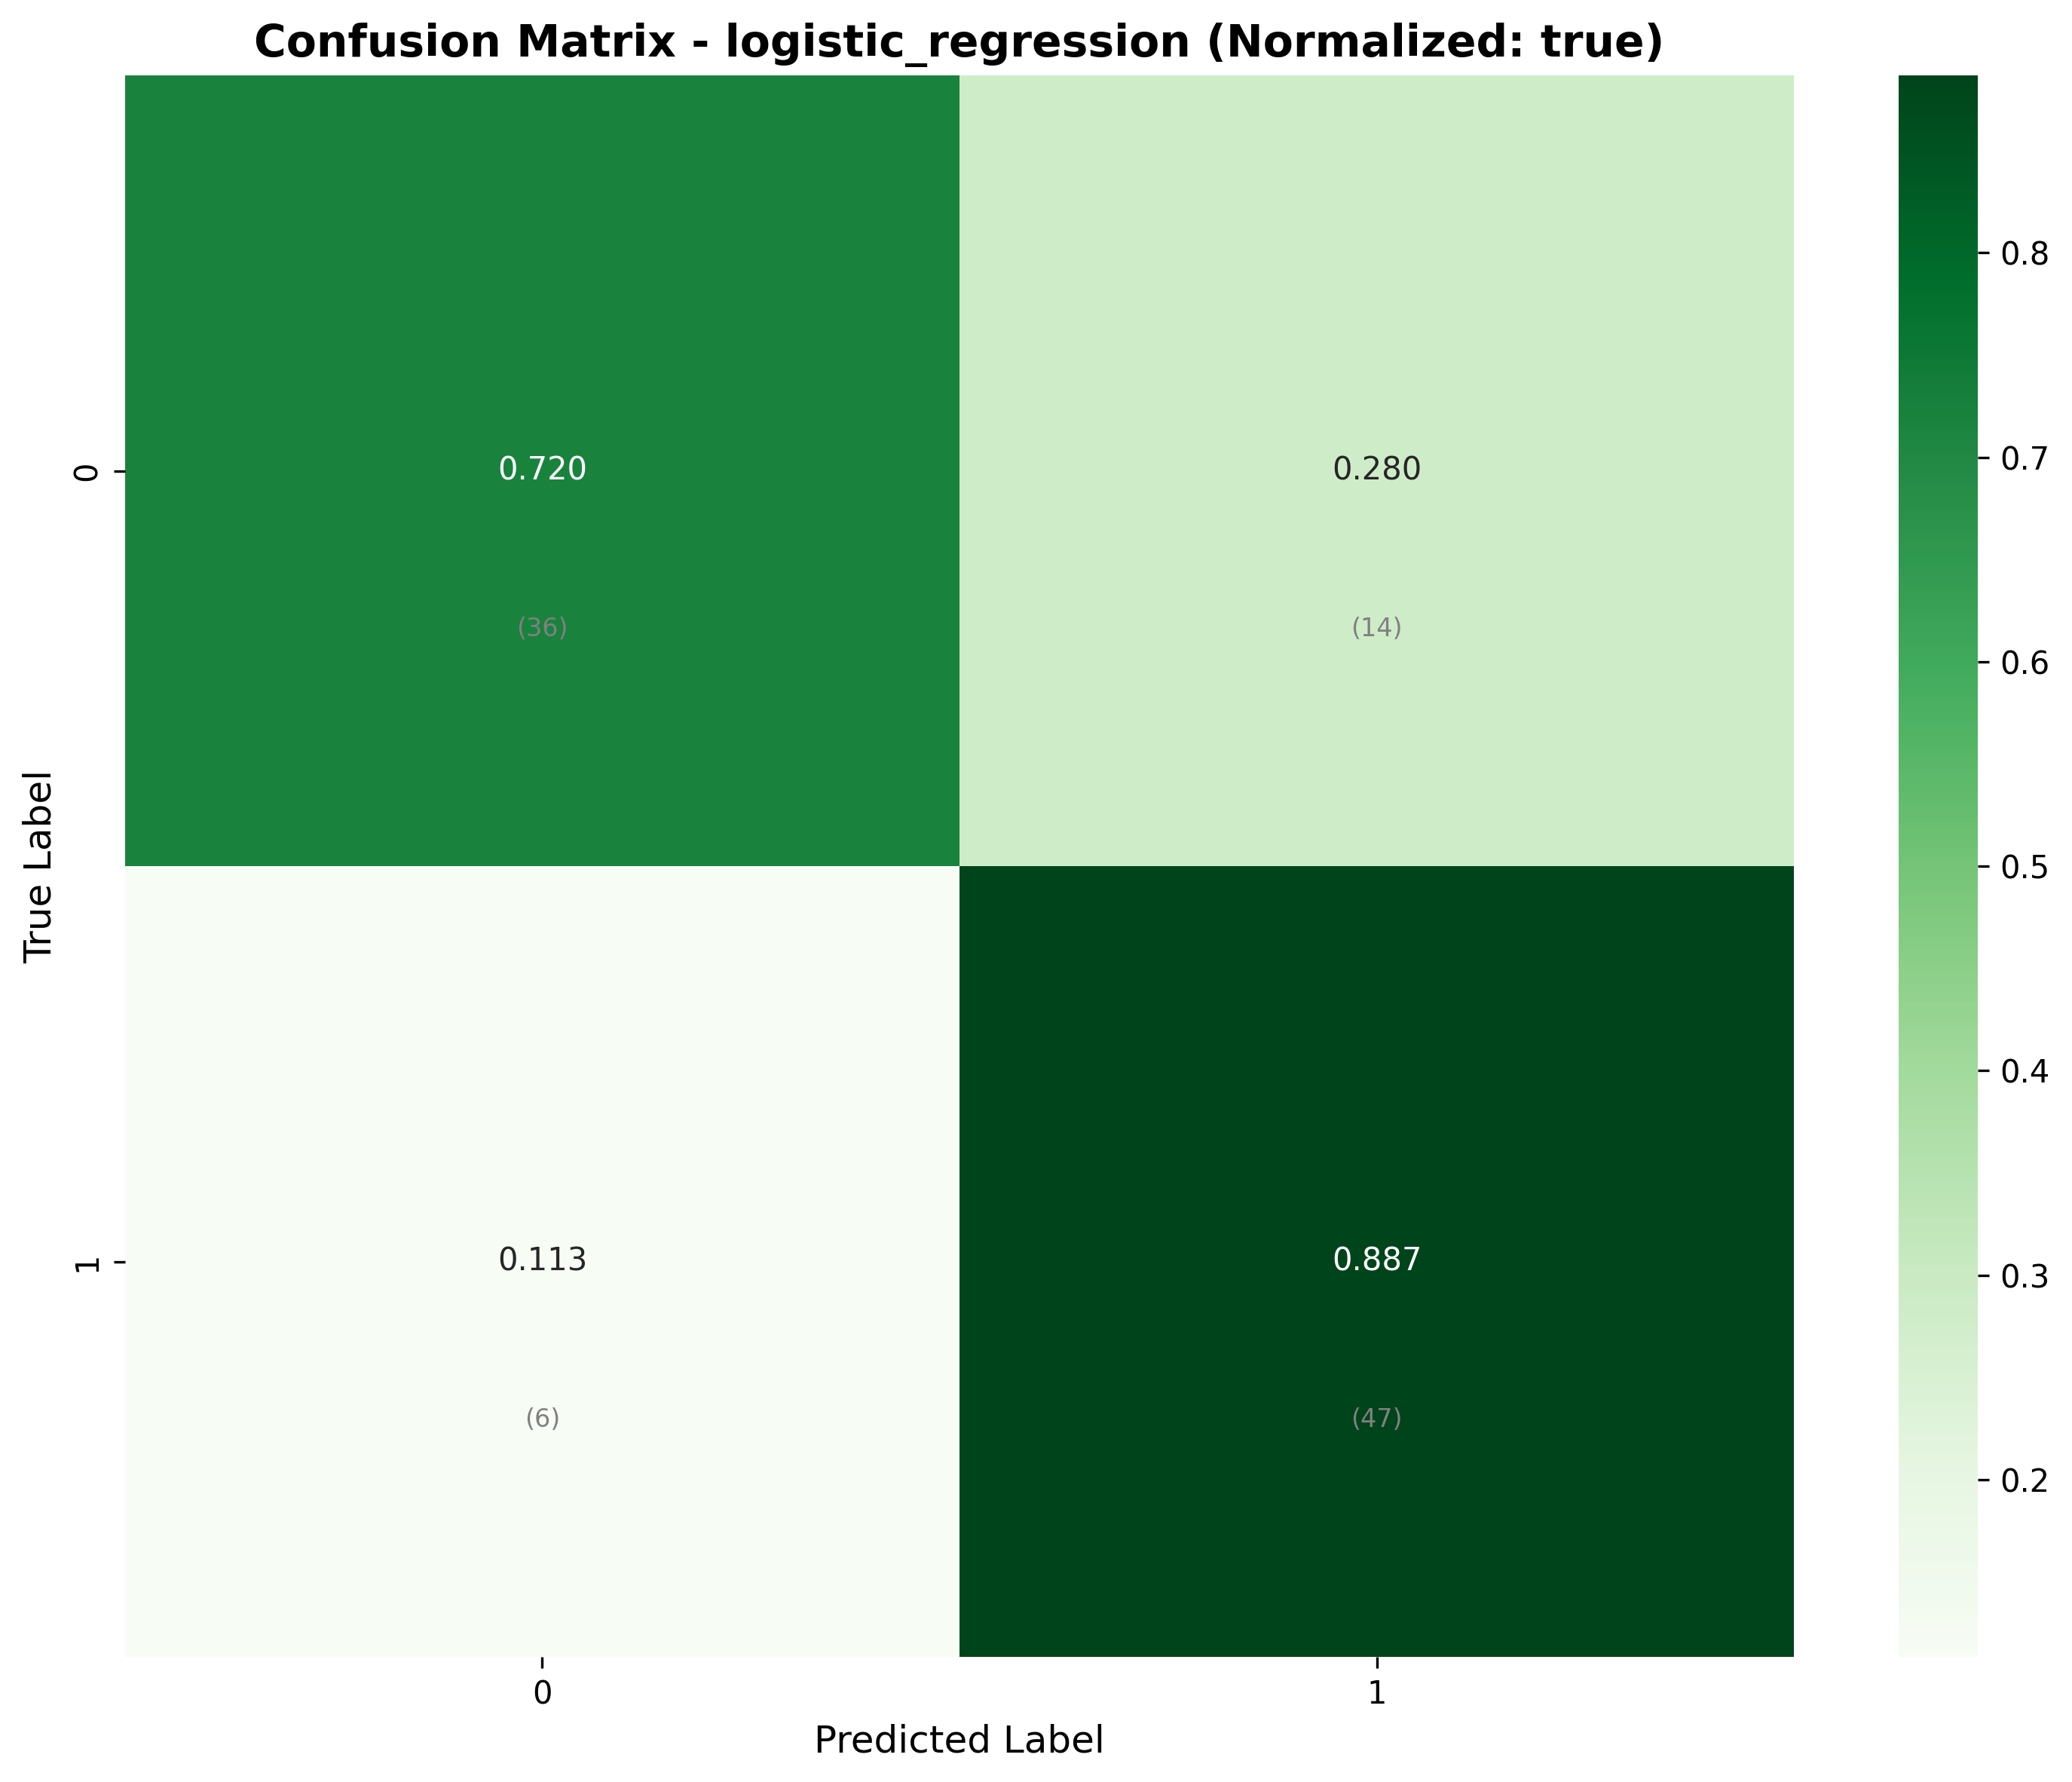
\includegraphics[width=0.95\textwidth]{Result/heart_dataset/confusion_matrices/logistic_regression_numeric_dataset_StandardScaler.png}
\caption{LR Heart Dataset}
\label{fig:lr_heart_confusion}
\end{subfigure}
\hfill
\begin{subfigure}[b]{0.31\textwidth}
\centering
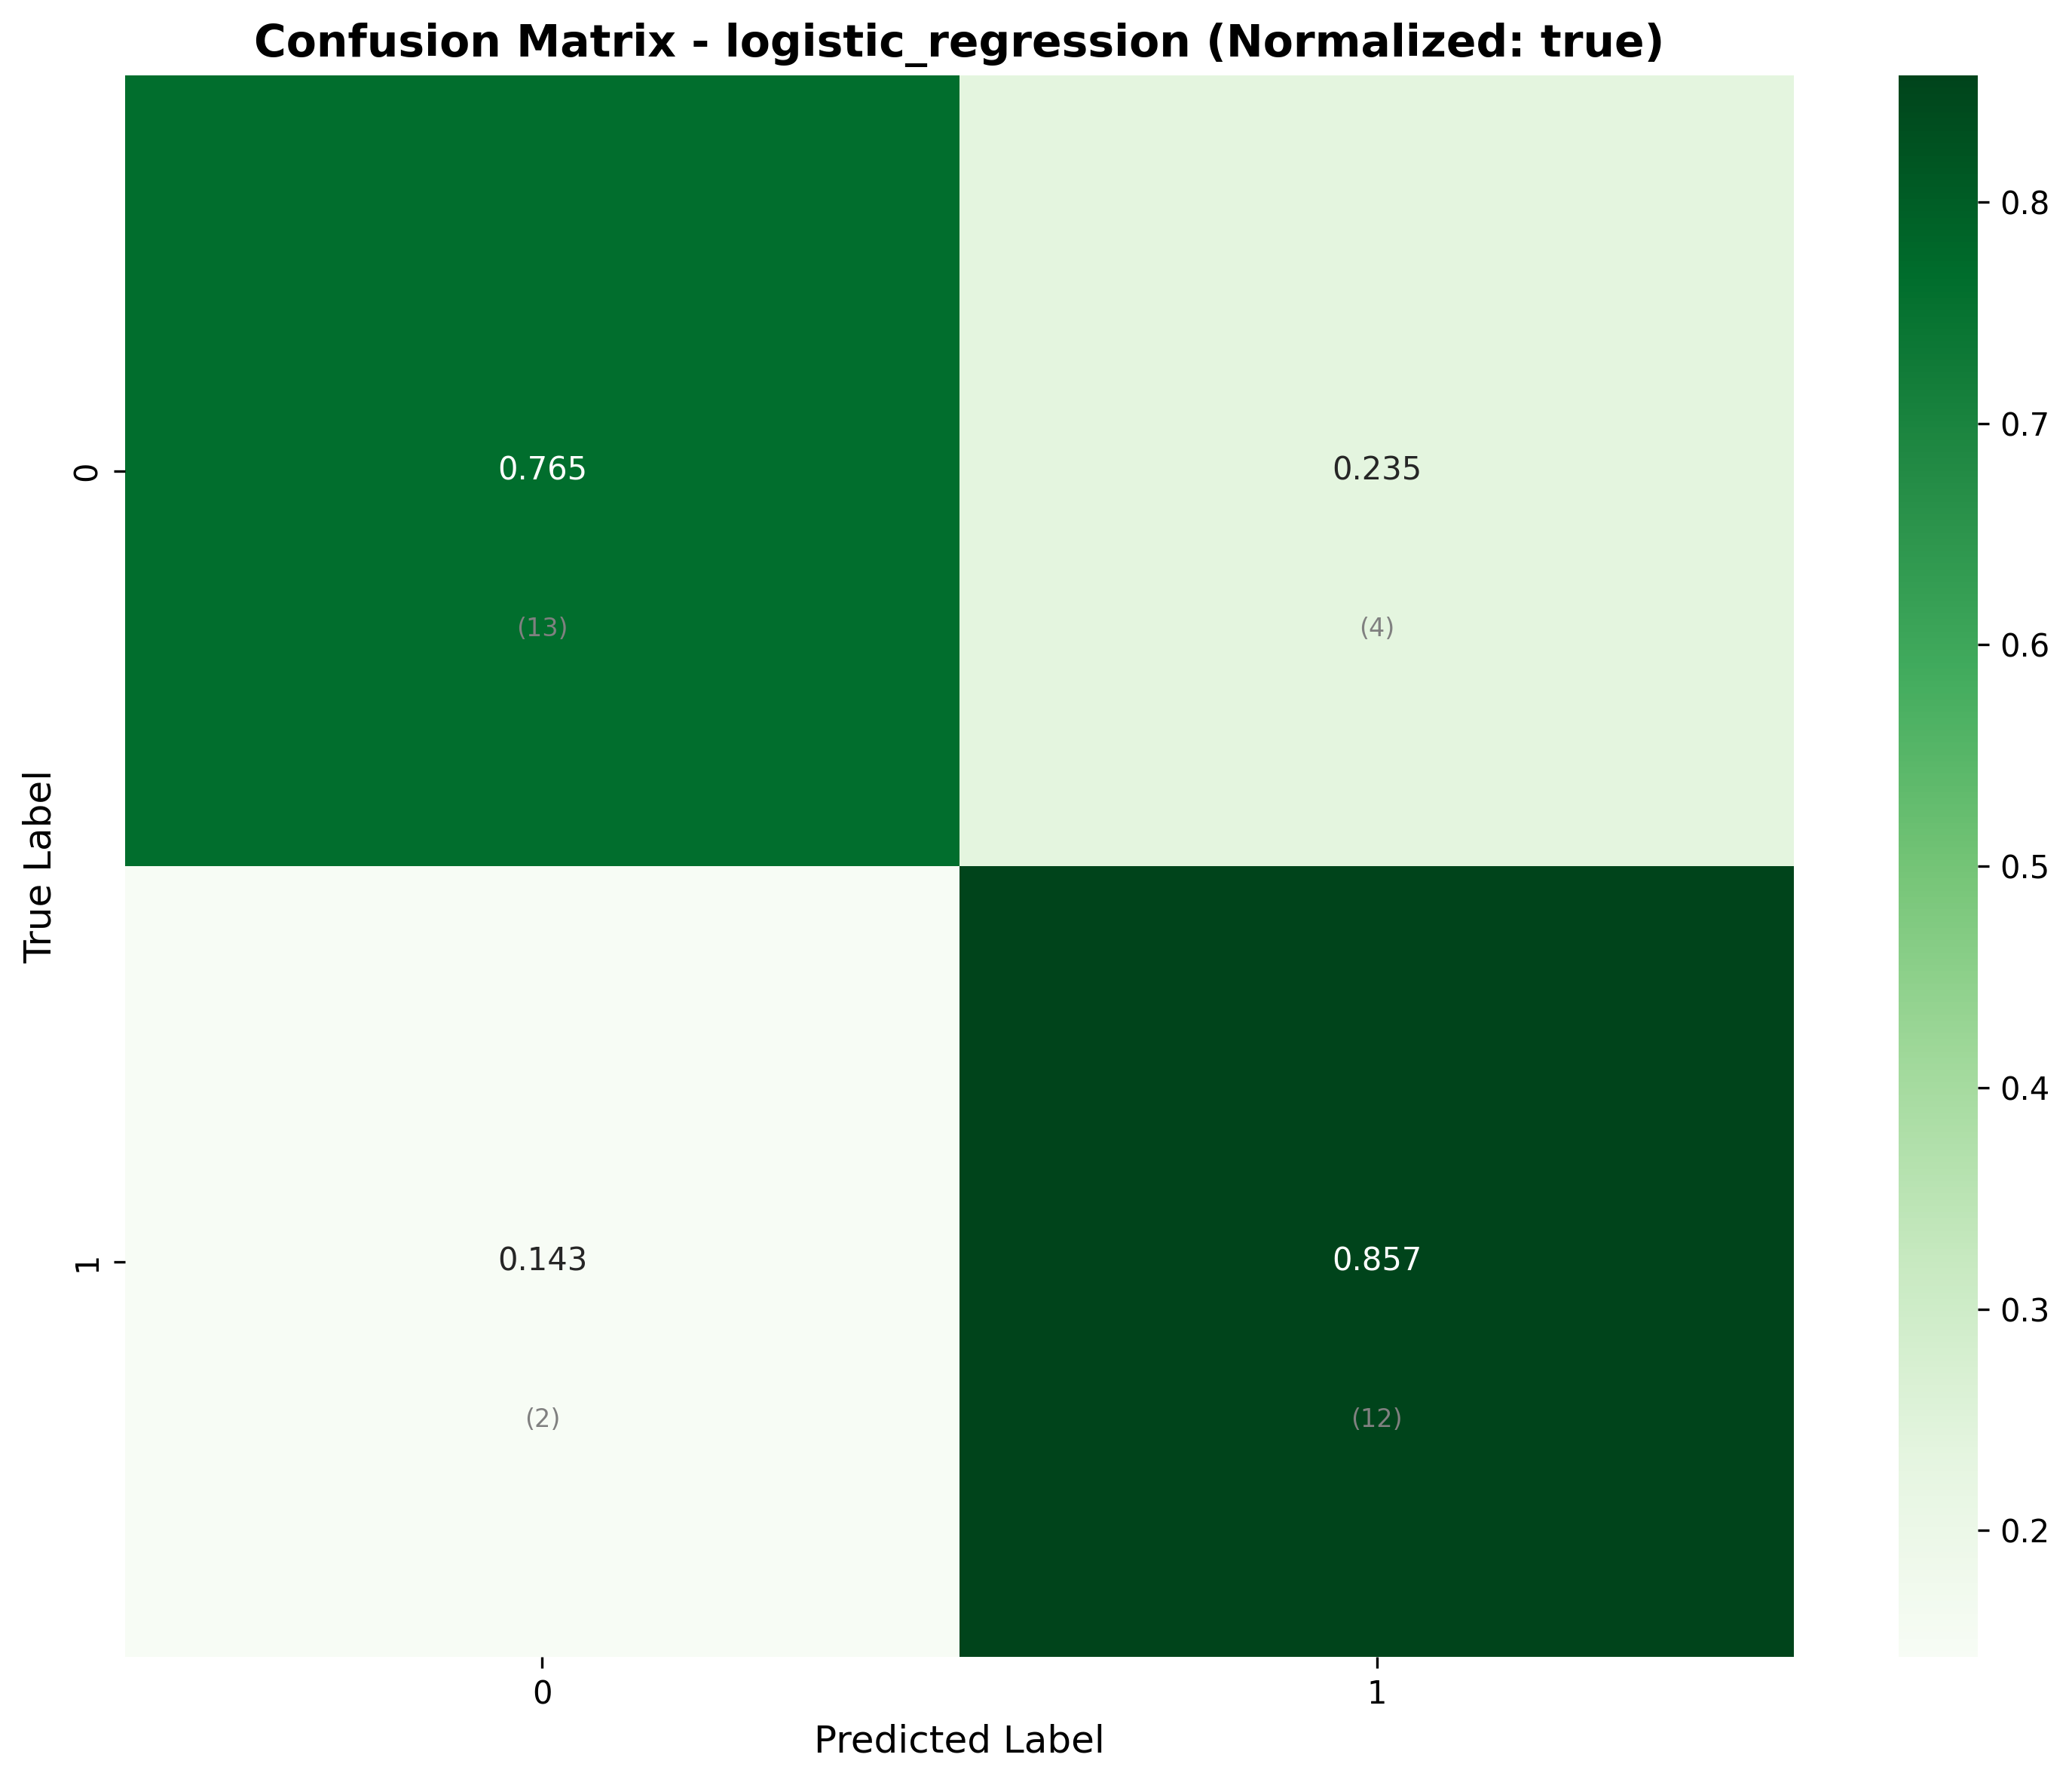
\includegraphics[width=0.95\textwidth]{Result/cleveland_dataset/confusion_matrices/logistic_regression_numeric_dataset_RobustScaler.png}
\caption{LR RobustScaler Performance}
\label{fig:lr_baseline_performance}
\end{subfigure}
\caption{Logistic Regression Cross-Dataset: Fast baseline với direct medical interpretation}
\label{fig:logistic_regression_complete}
\end{figure}

\textbf{SVM}: Dramatic scaler sensitivity observed: RobustScaler tốt nhất với Cleveland (90.3\%), cải thiện đáng kể trên Heart Dataset. SVM performance variation này phản ánh sensitivity đến outliers trong medical data - RobustScaler resistant to extreme cholesterol values hoặc blood pressure measurements using median và quartiles thay vì mean/variance.

\begin{figure}[H]
\centering
\begin{subfigure}[b]{0.31\textwidth}
\centering
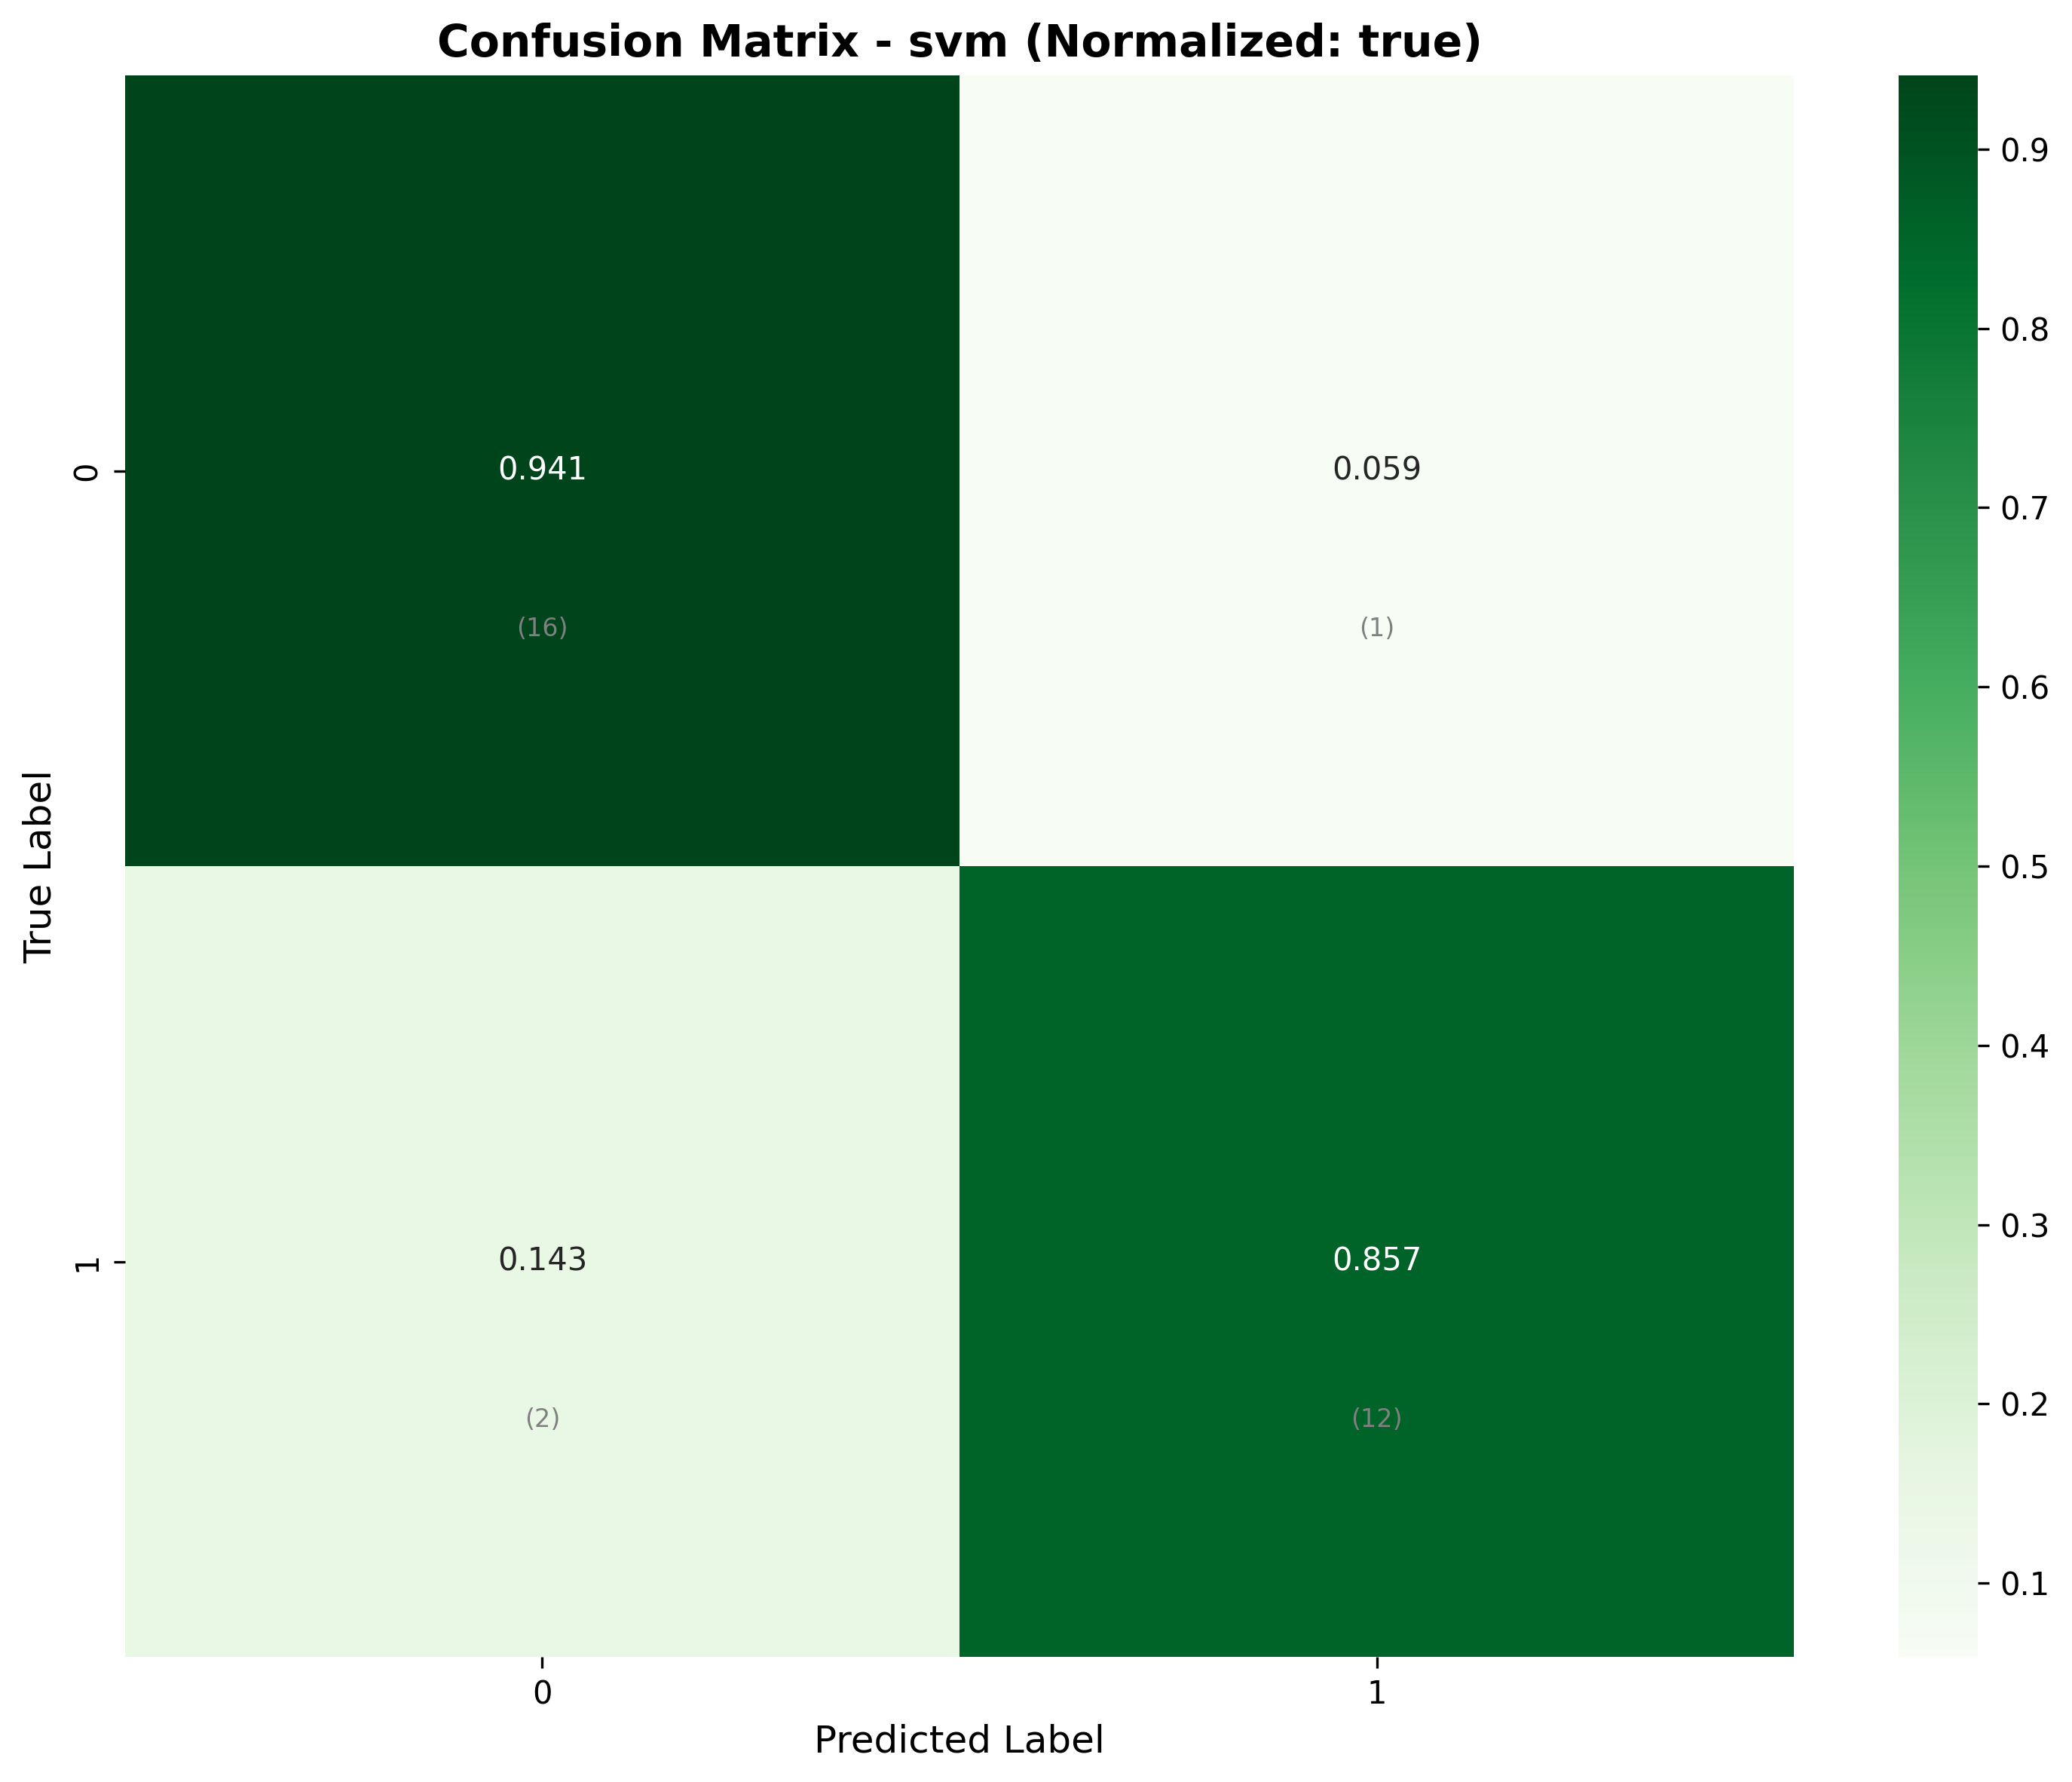
\includegraphics[width=0.95\textwidth]{Result/cleveland_dataset/confusion_matrices/svm_numeric_dataset_RobustScaler.png}
\caption{SVM RobustScaler (90.3\%)}
\label{fig:svm_robust_optimal}
\end{subfigure}
\hfill
\begin{subfigure}[b]{0.31\textwidth}
\centering
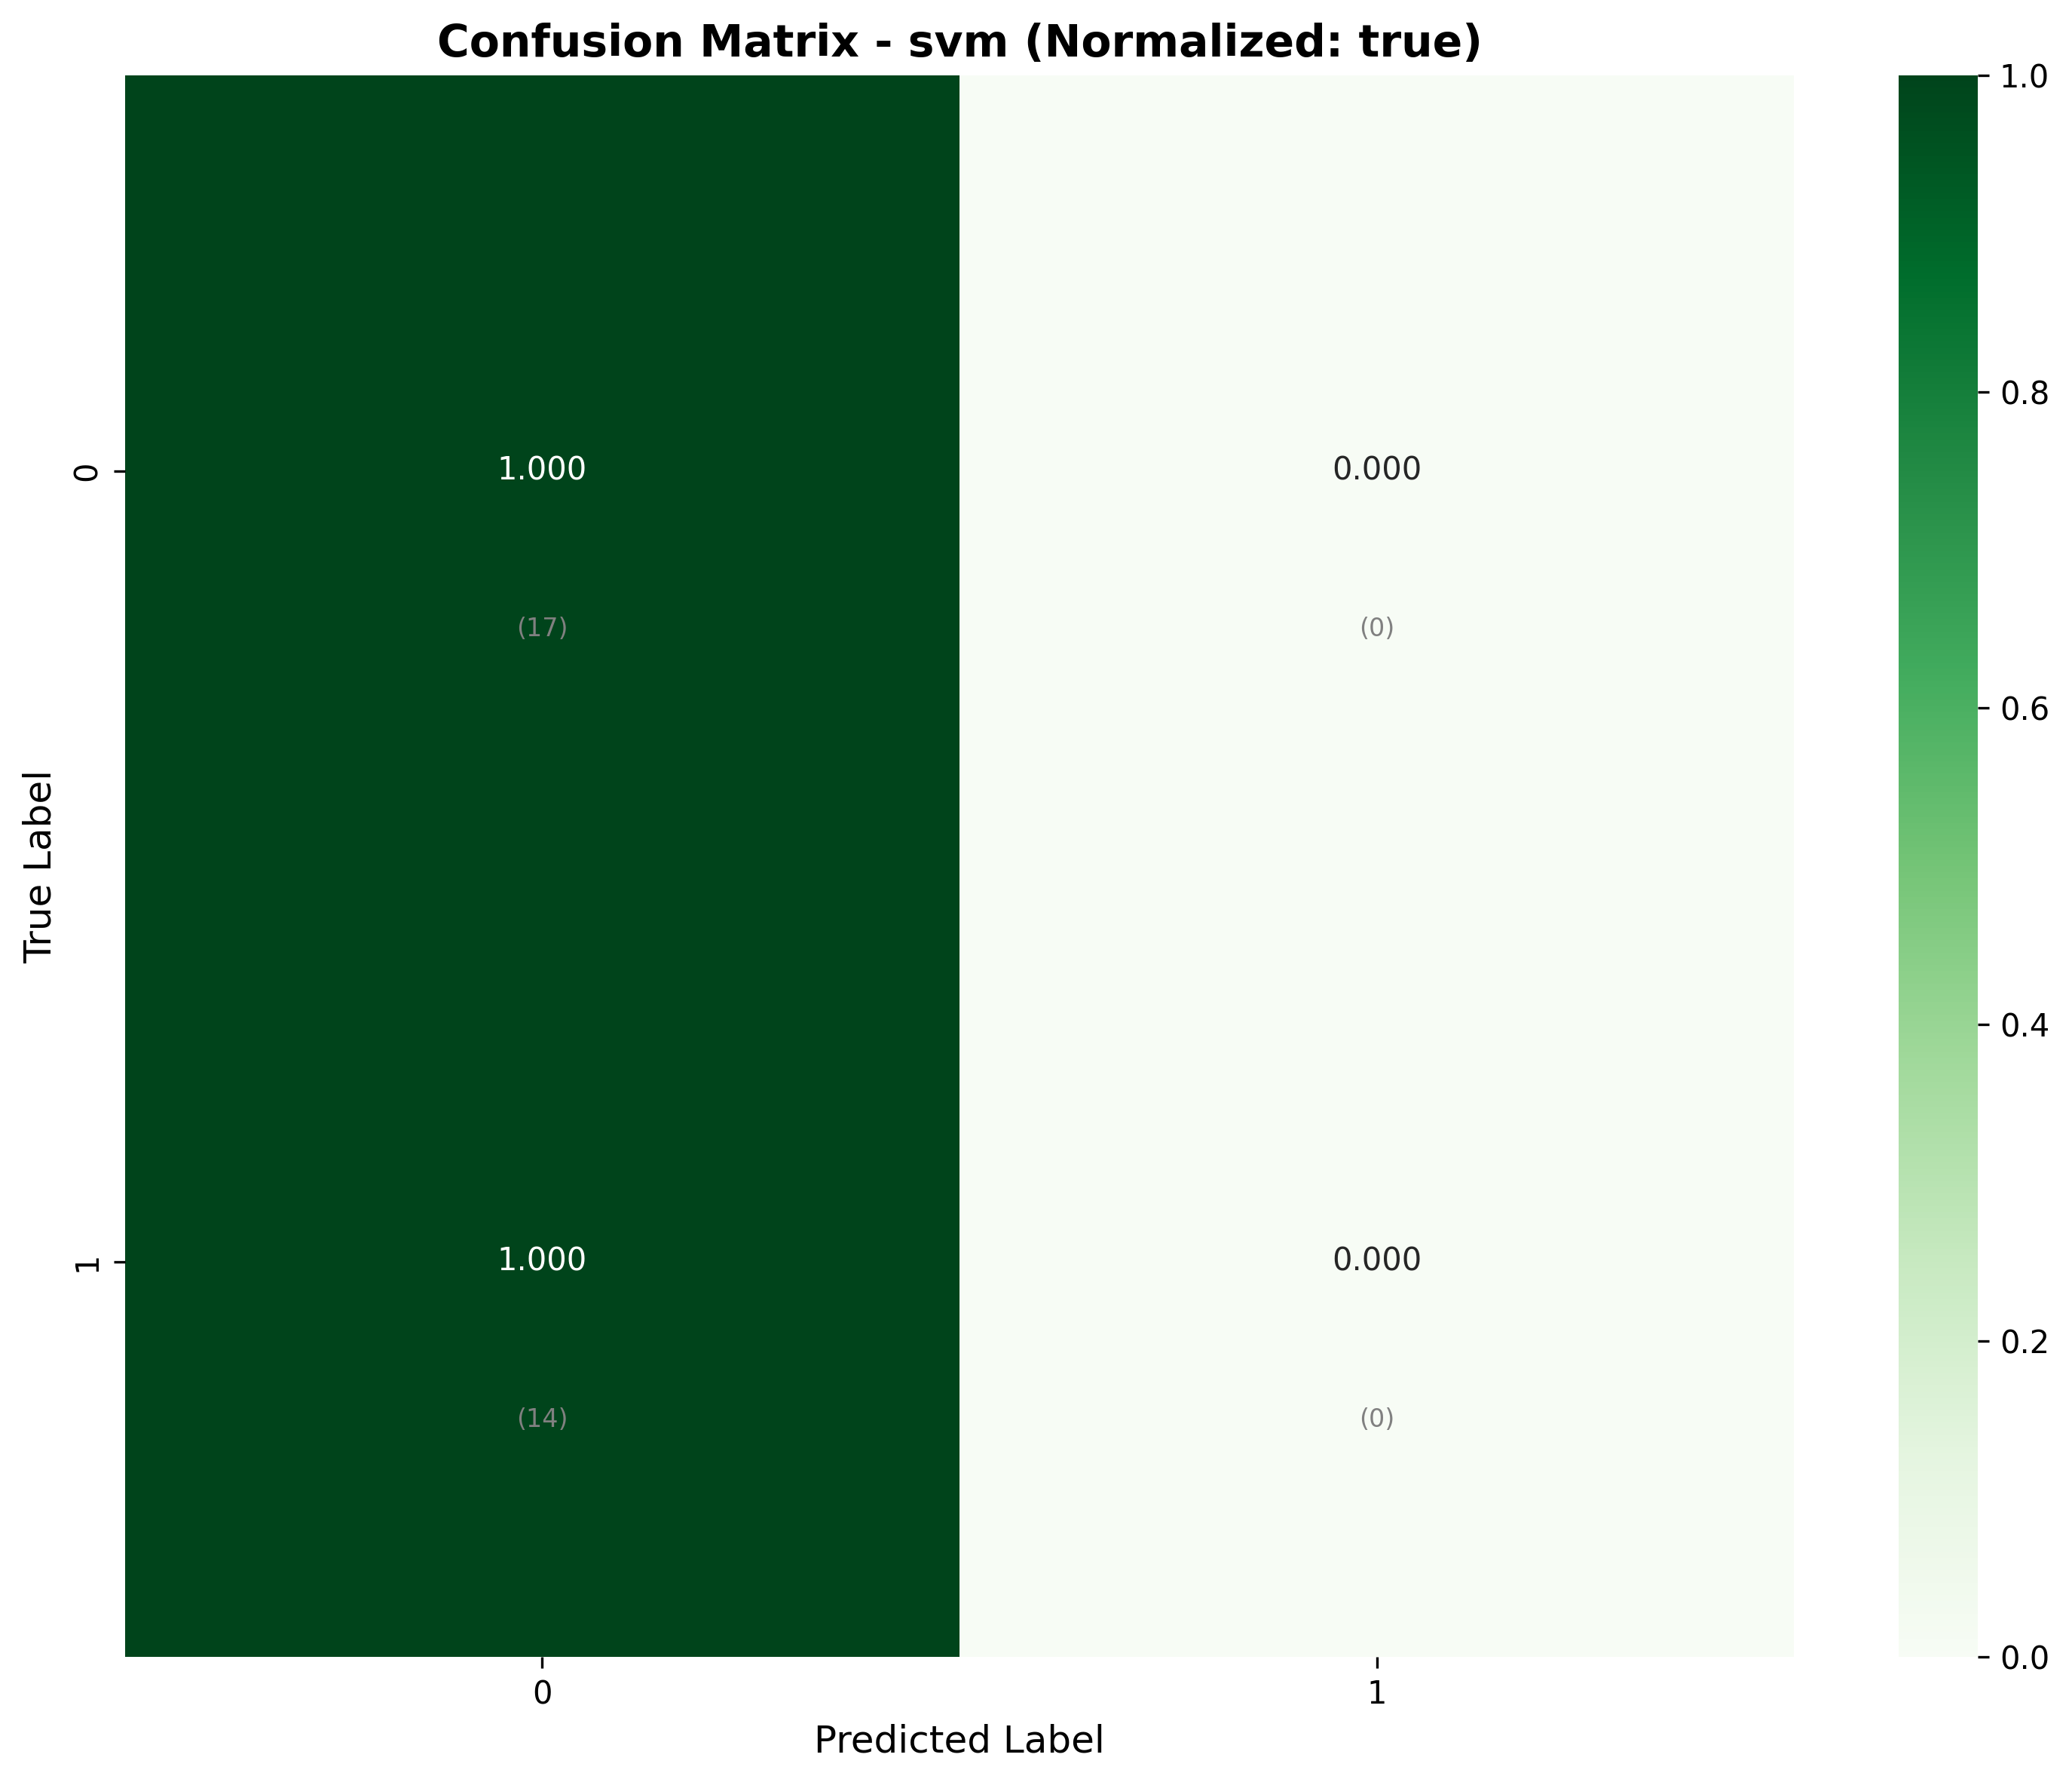
\includegraphics[width=0.95\textwidth]{Result/cleveland_dataset/confusion_matrices/svm_numeric_dataset_MinMaxScaler.png}
\caption{SVM MinMaxScaler (54.8\%)}
\label{fig:svm_minmax_degraded}
\end{subfigure}
\hfill
\begin{subfigure}[b]{0.31\textwidth}
\centering
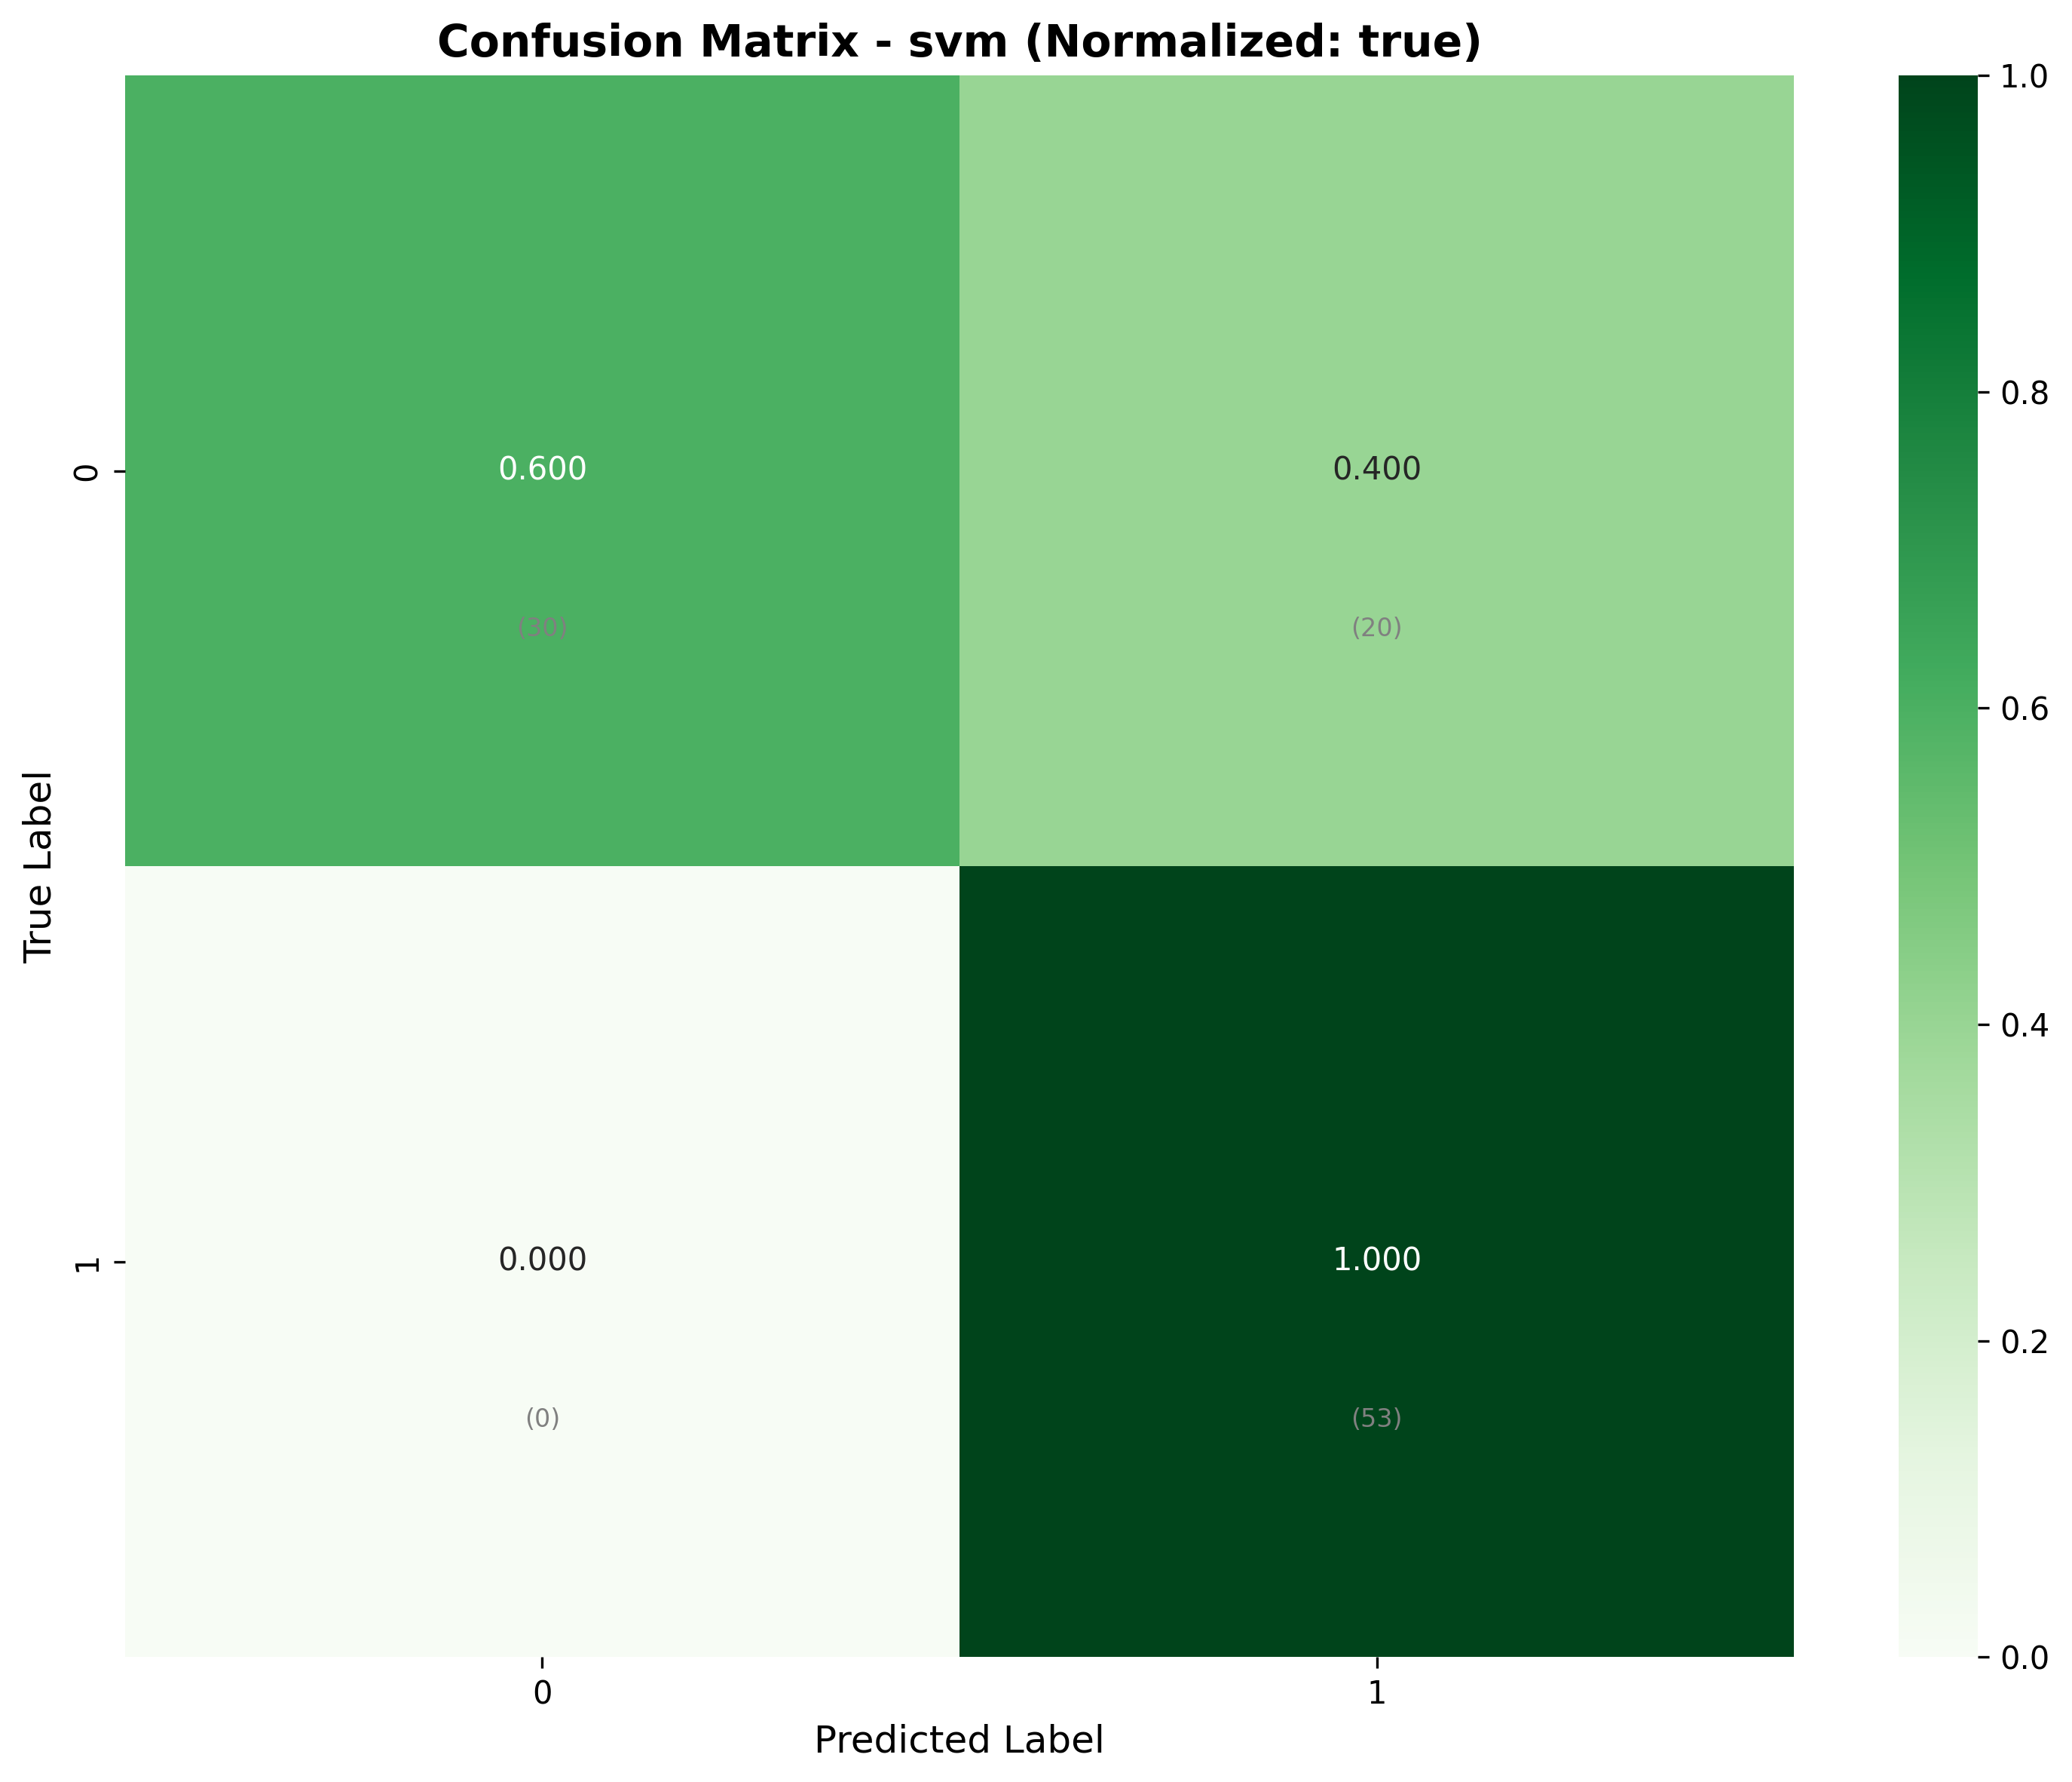
\includegraphics[width=0.95\textwidth]{Result/heart_dataset/confusion_matrices/svm_numeric_dataset_RobustScaler.png}
\caption{SVM RobustScaler Heart}
\label{fig:svm_heart_performance}
\end{subfigure}
\caption{SVM Scaler Sensitivity: RobustScaler optimal cho clinical outliers vs MinMaxScaler degradation}
\label{fig:svm_scaler_comparison}
\end{figure}

Hình \ref{fig:svm_scaler_comparison} chứng minh tầm quan trọng quan trọng của lựa chọn tiền xử lý trong ML y tế với biến thiên hiệu suất nghiêm trọng từ 54.8\% (MinMaxScaler) đến 90.3\% (RobustScaler).

\textbf{KNN}: Phân loại dựa trên khoảng cách hoạt động tốt hơn với dataset lớn hơn, StandardScaler tối ưu cho tính toán khoảng cách Euclidean (phạm vi 74.2-87.1\%). KNN nhấn mạnh việc phân nhóm phenotype lâm sàng thông qua dự đoán dựa trên khoảng cách, hữu ích cho việc xác định các profile rủi ro bệnh nhân tương tự.

\begin{figure}[H]
\centering
\begin{subfigure}[b]{0.31\textwidth}
\centering
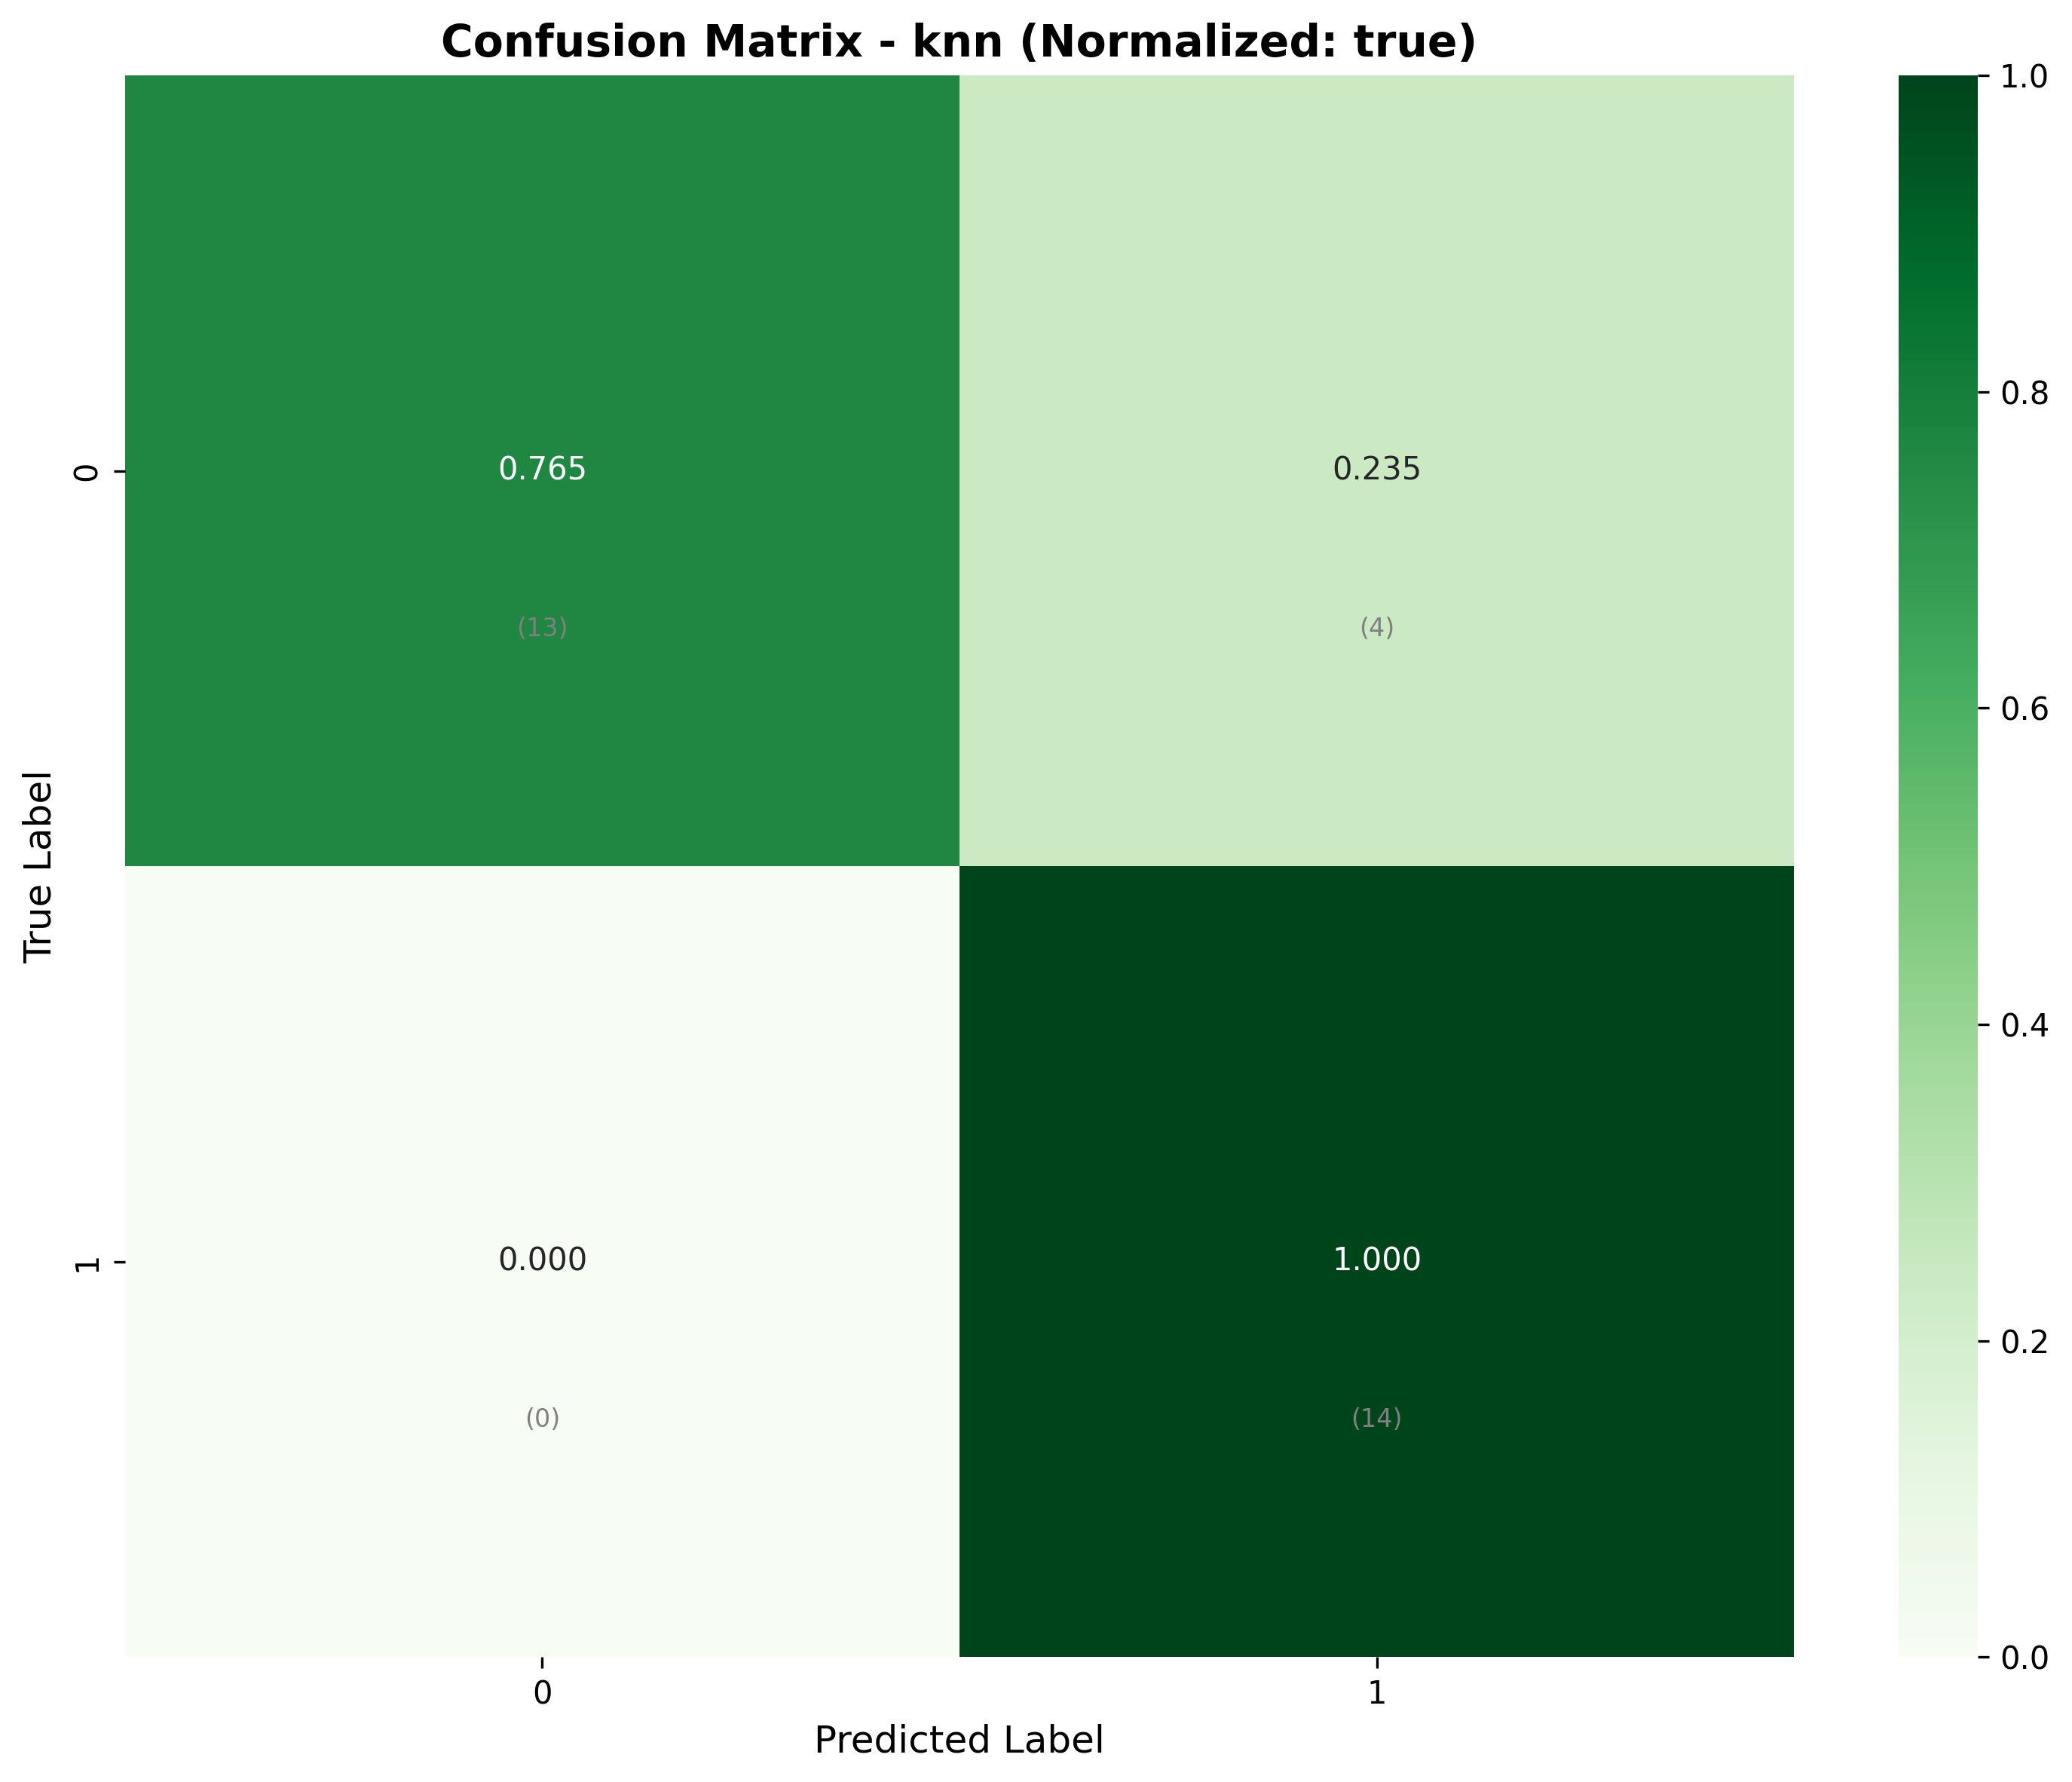
\includegraphics[width=0.95\textwidth]{Result/cleveland_dataset/confusion_matrices/knn_numeric_dataset_StandardScaler.png}
\caption{KNN StandardScaler (87.1\%)}
\label{fig:knn_standard_performance}
\end{subfigure}
\hfill
\begin{subfigure}[b]{0.31\textwidth}
\centering
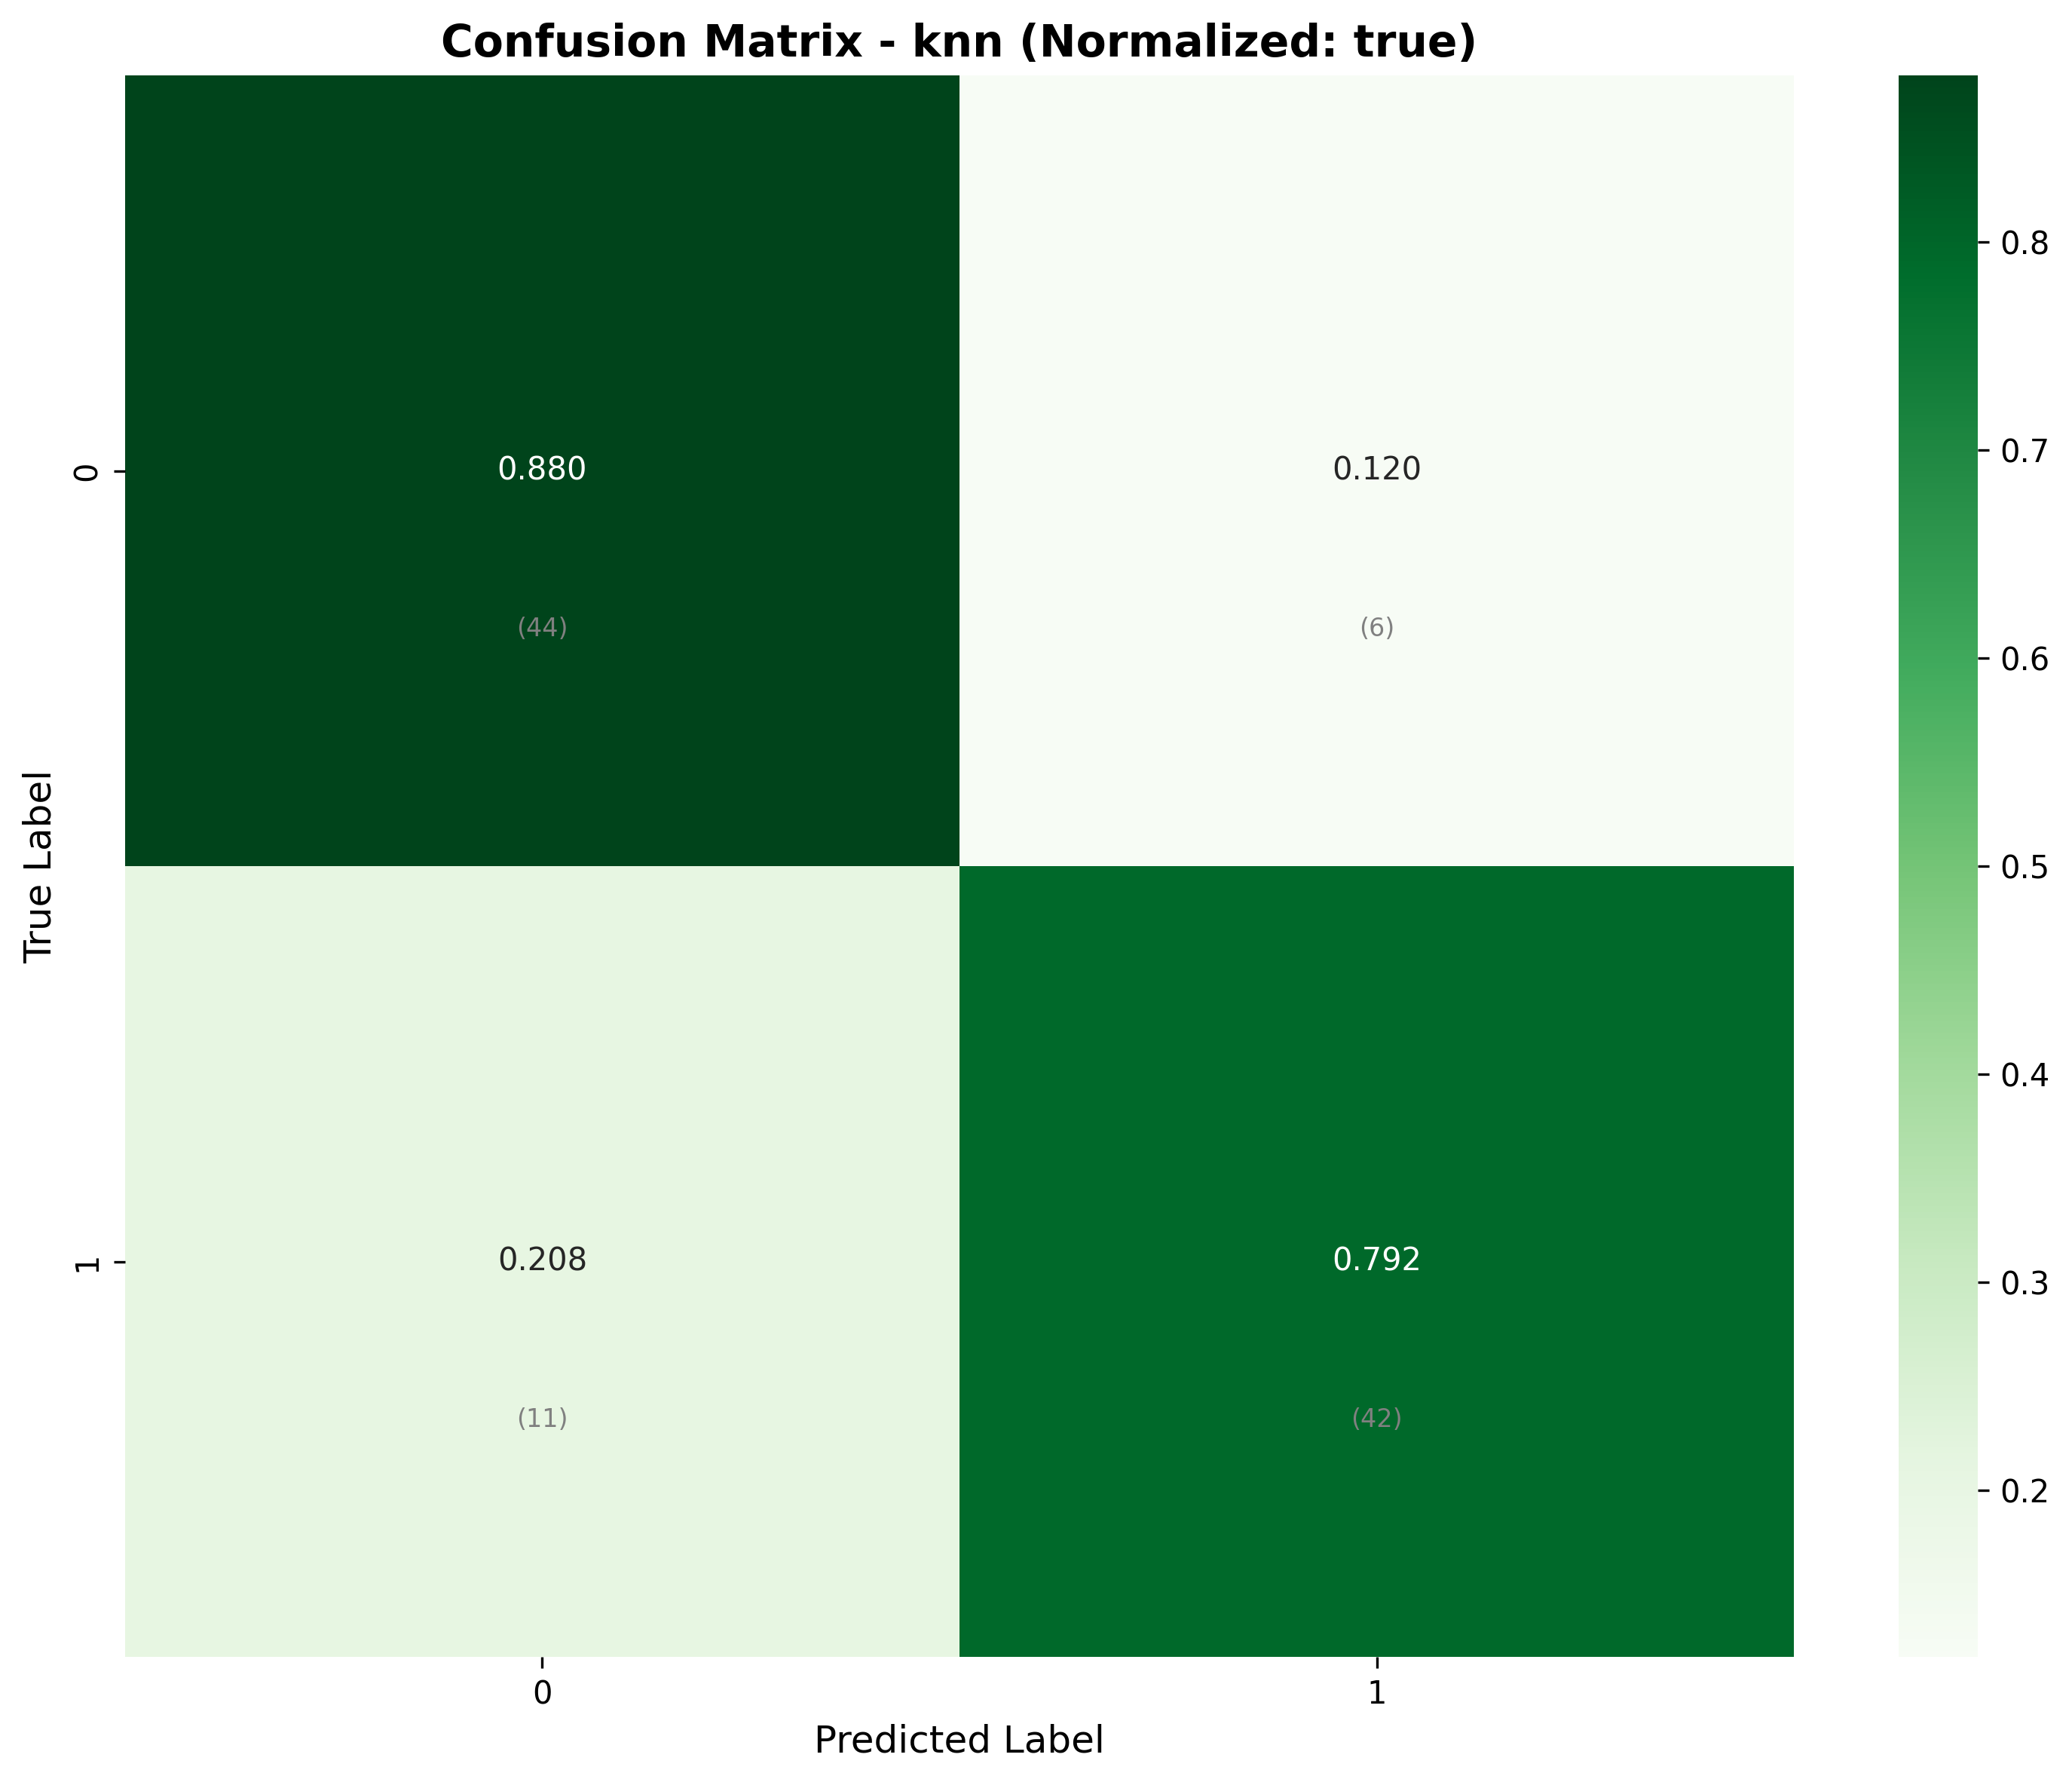
\includegraphics[width=0.95\textwidth]{Result/heart_dataset/confusion_matrices/knn_numeric_dataset_StandardScaler.png}
\caption{KNN Heart Dataset}
\label{fig:knn_heart_performance}
\end{subfigure}
\hfill
\begin{subfigure}[b]{0.31\textwidth}
\centering
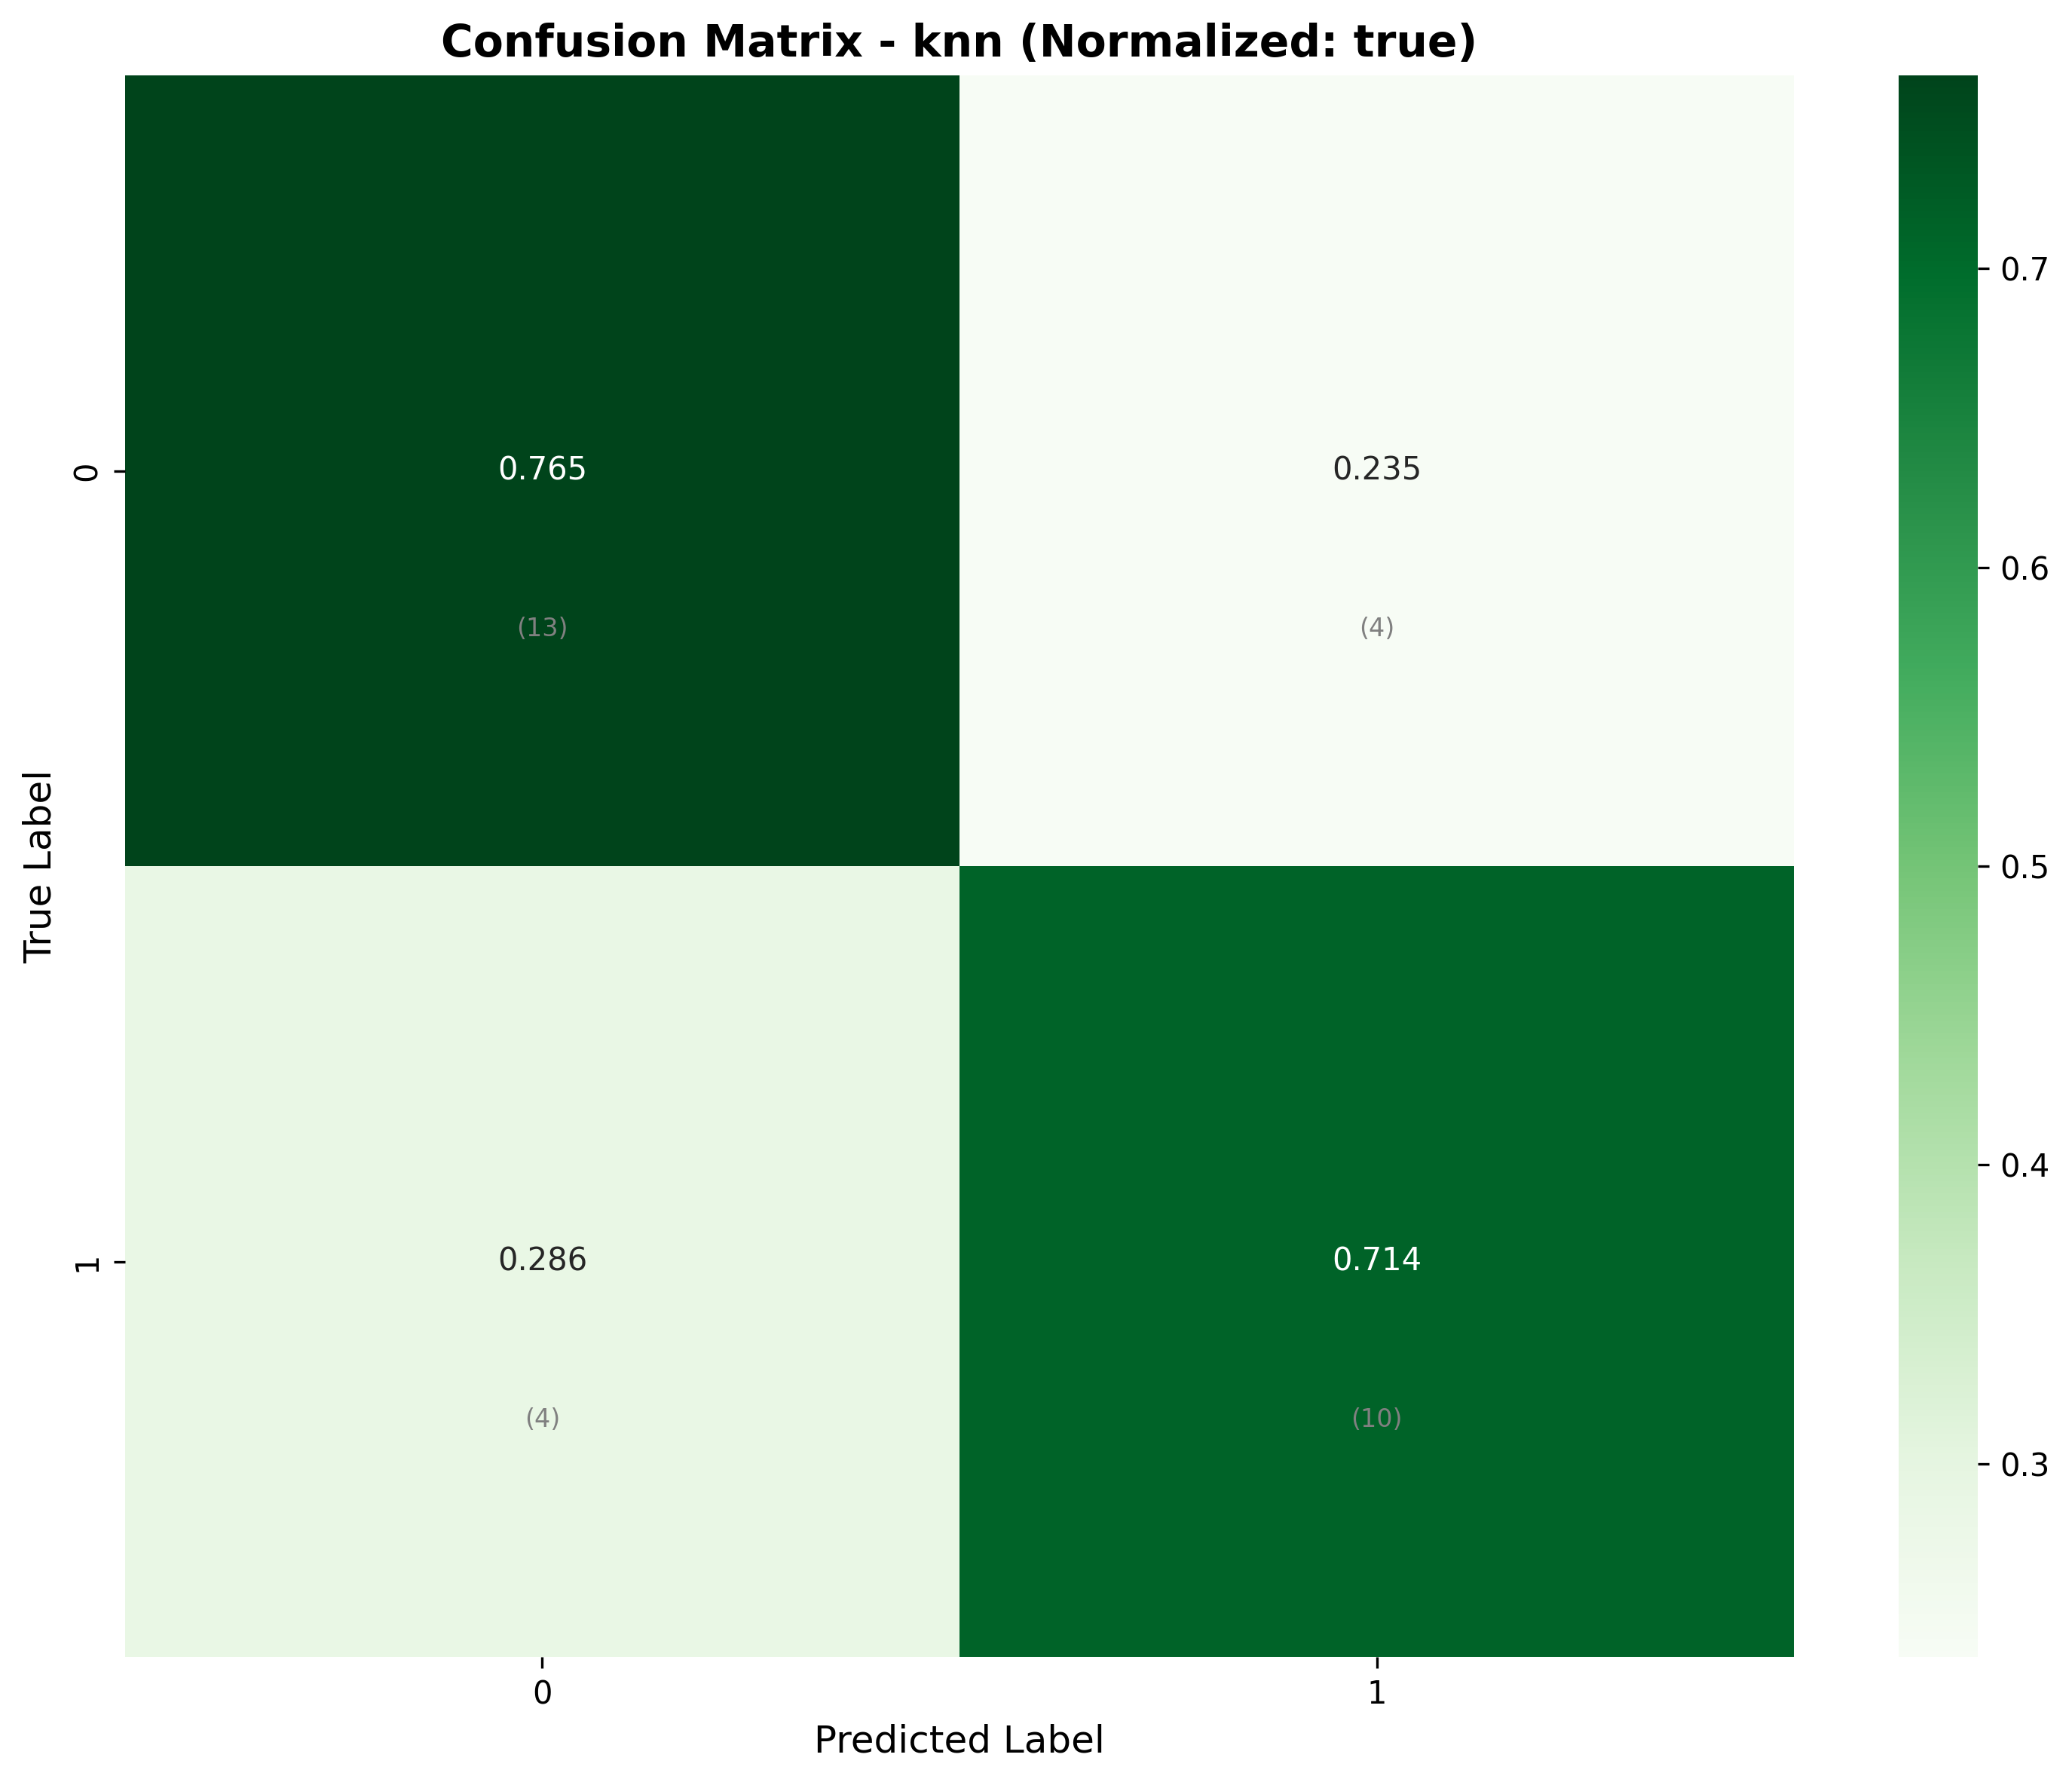
\includegraphics[width=0.95\textwidth]{Result/cleveland_dataset/confusion_matrices/knn_numeric_dataset_MinMaxScaler.png}
\caption{KNN MinMaxScaler (74.2\%)}
\label{fig:knn_minmax_performance}
\end{subfigure}
\caption{KNN Scaler Sensitivity: Distance-based algorithms advantage với proper scaling}
\label{fig:knn_analysis_complete}
\end{figure}

\textbf{Naive Bayes}: Độ chính xác nhất quán 83.9\% với training cực kỳ nhanh (<0.02 giây), independence assumption phù hợp cho cardiac risk factors. Ưu điểm của Naive Bayes classifier bao gồm probabilistic framework cho uncertainty quantification và direct Bayesian interpretation trong bối cảnh clinical decision-making.

\begin{figure}[H]
\centering
\begin{subfigure}[b]{0.31\textwidth}
\centering
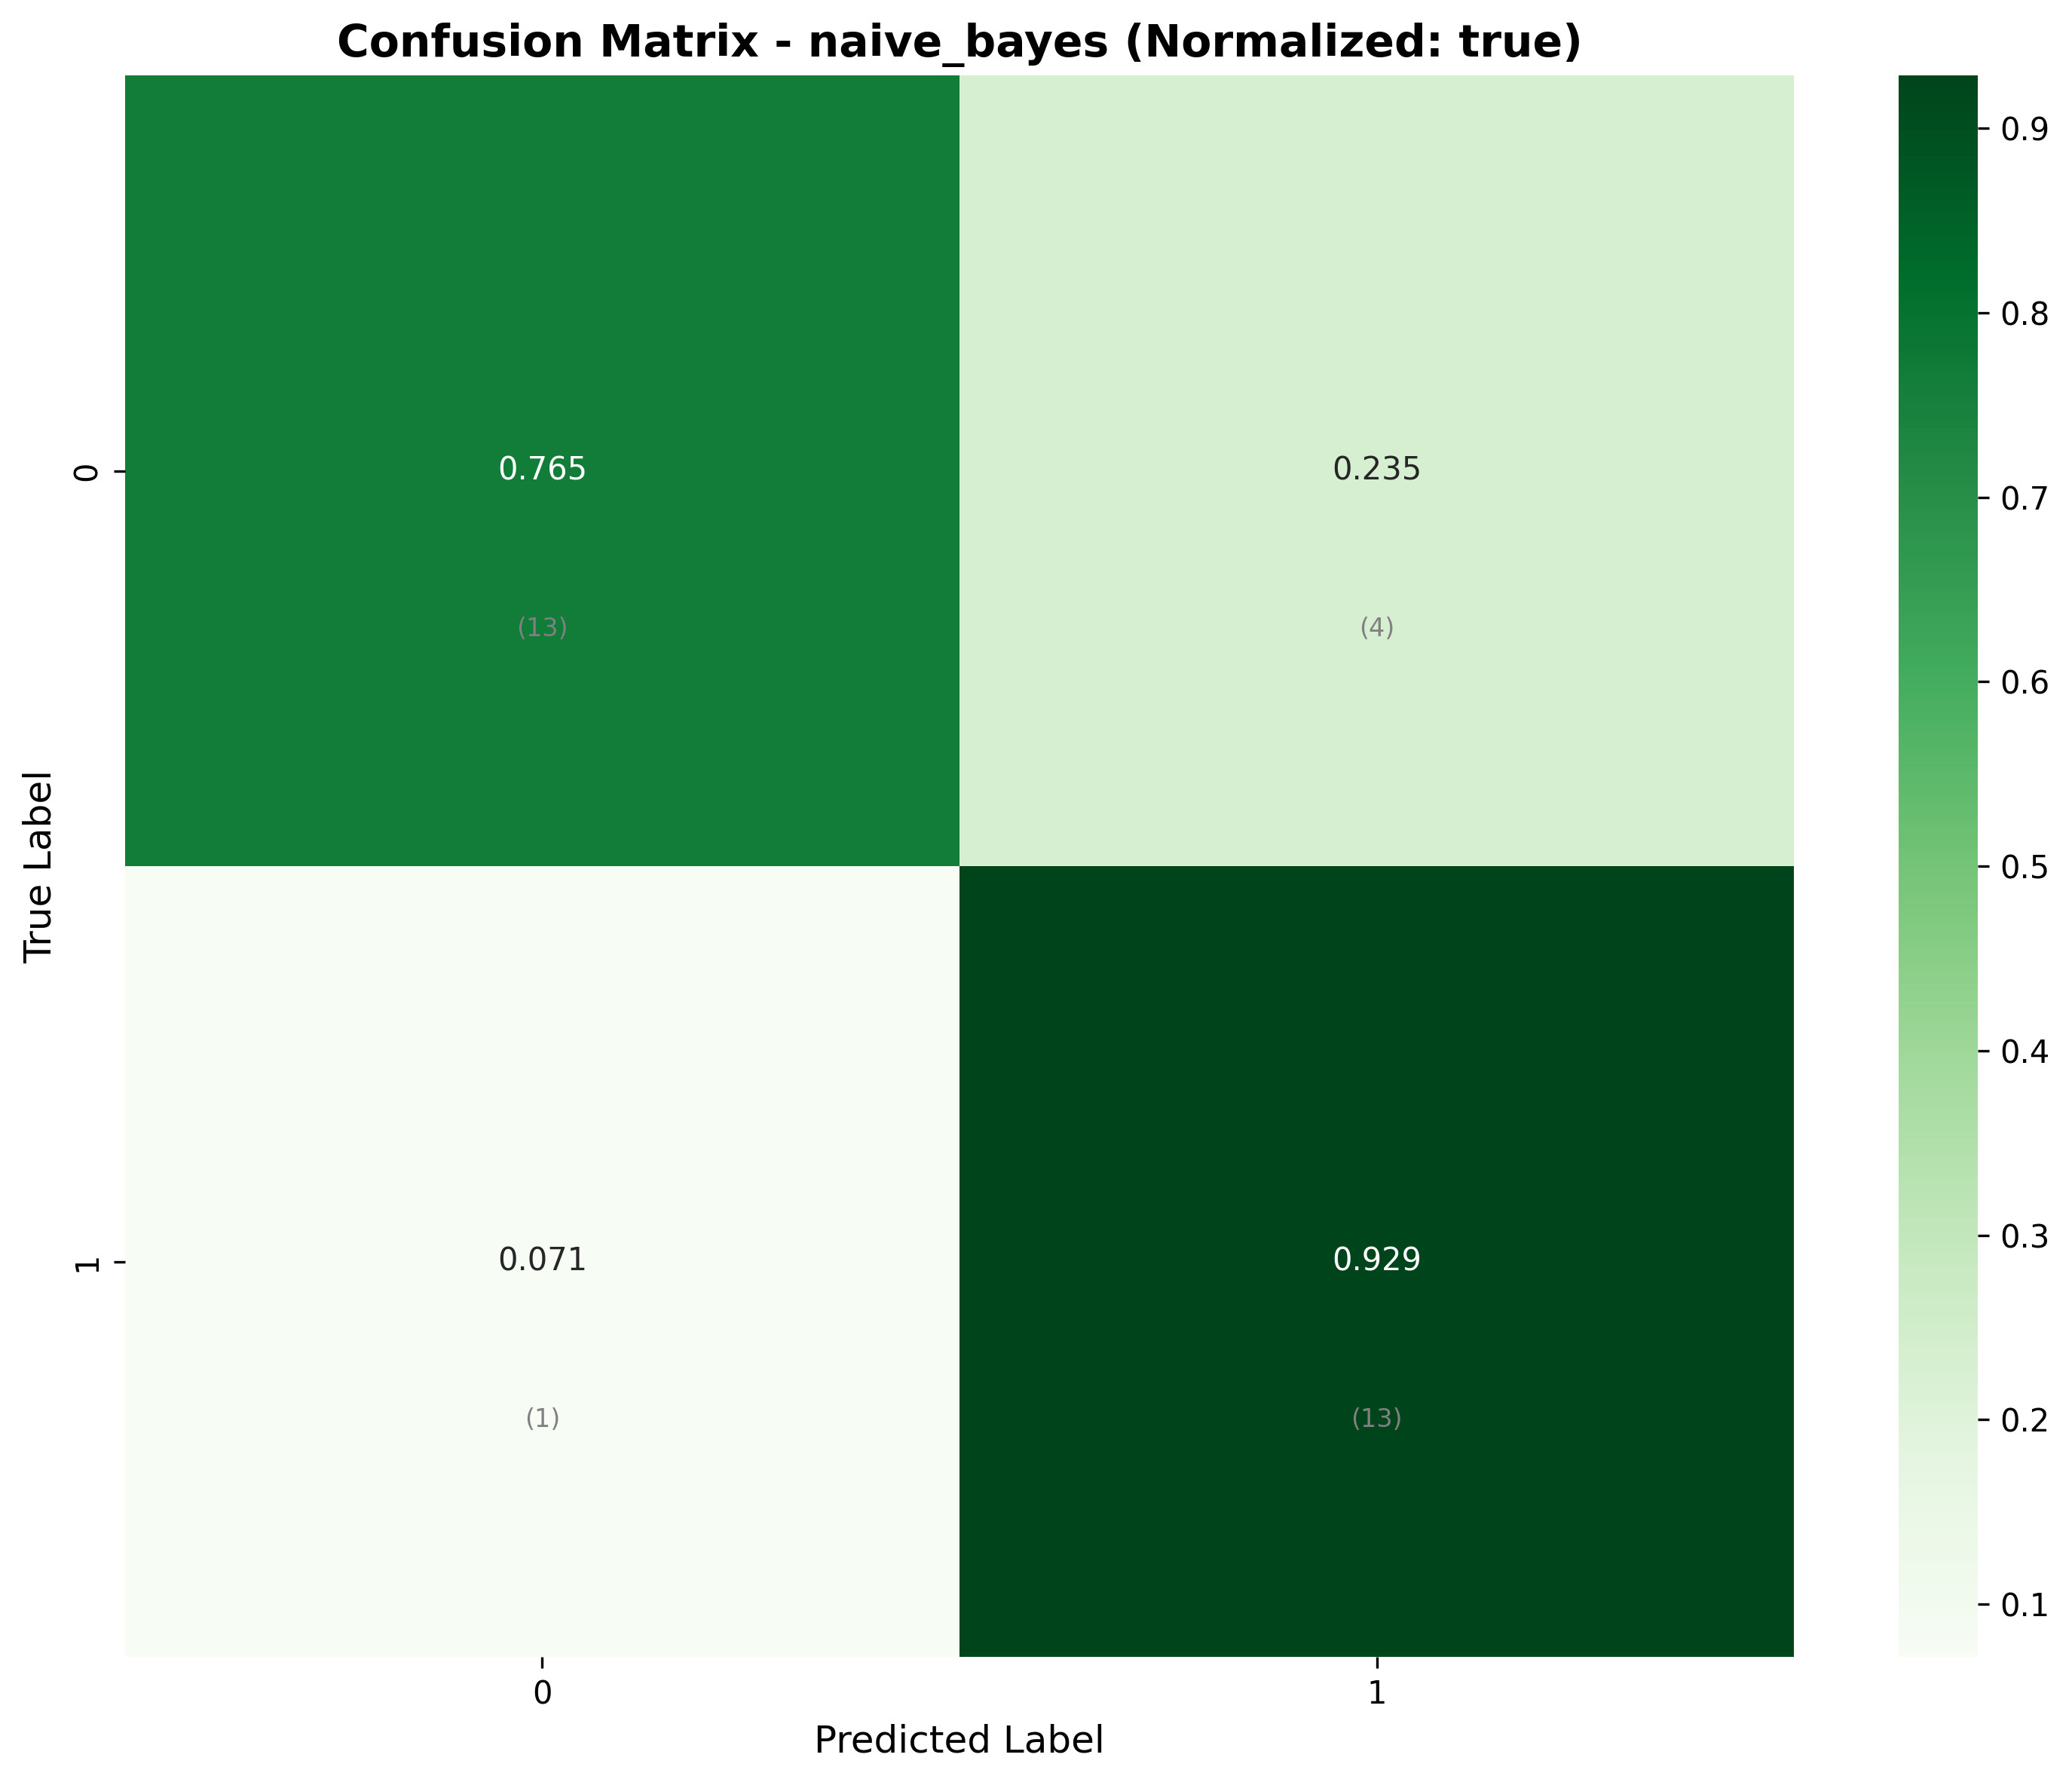
\includegraphics[width=0.95\textwidth]{Result/cleveland_dataset/confusion_matrices/naive_bayes_numeric_dataset_StandardScaler.png}
\caption{Naive Bayes Cleveland (83.9\%)}
\label{fig:nb_cleveland_performance}
\end{subfigure}
\hfill
\begin{subfigure}[b]{0.31\textwidth}
\centering
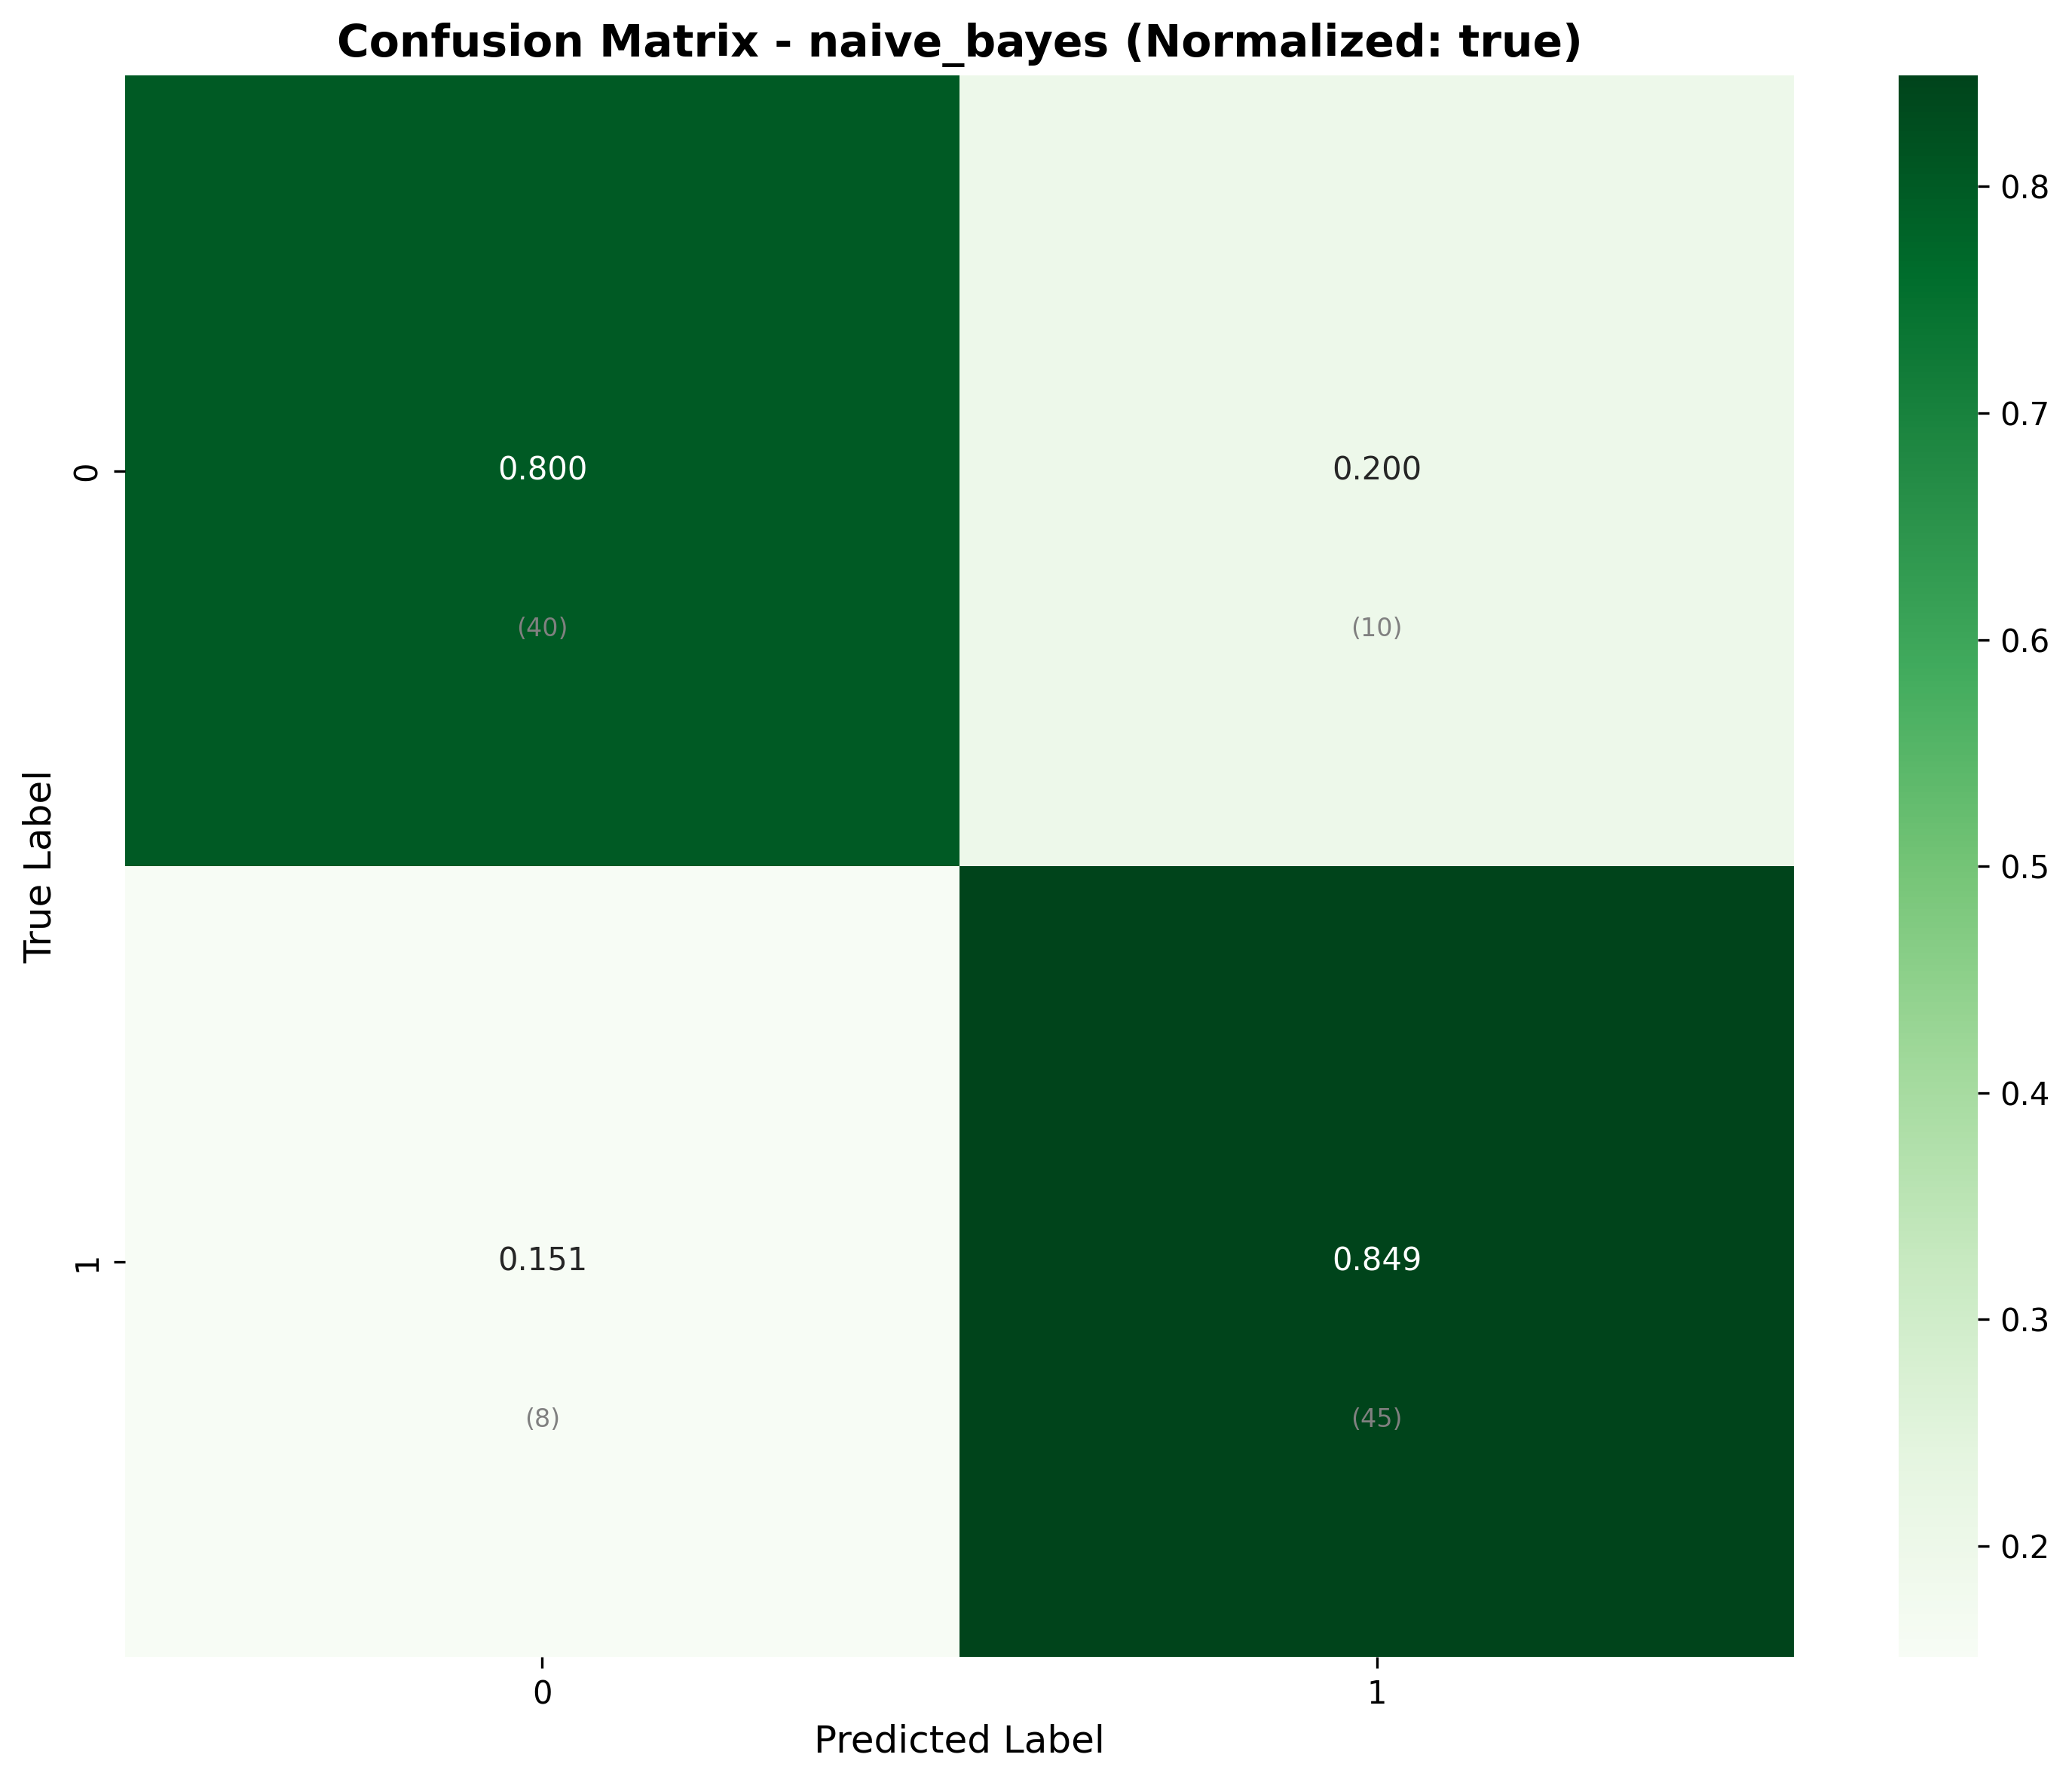
\includegraphics[width=0.95\textwidth]{Result/heart_dataset/confusion_matrices/naive_bayes_numeric_dataset_StandardScaler.png}
\caption{Naive Bayes Heart Dataset}
\label{fig:nb_heart_performance}
\end{subfigure}
\hfill
\begin{subfigure}[b]{0.31\textwidth}
\centering
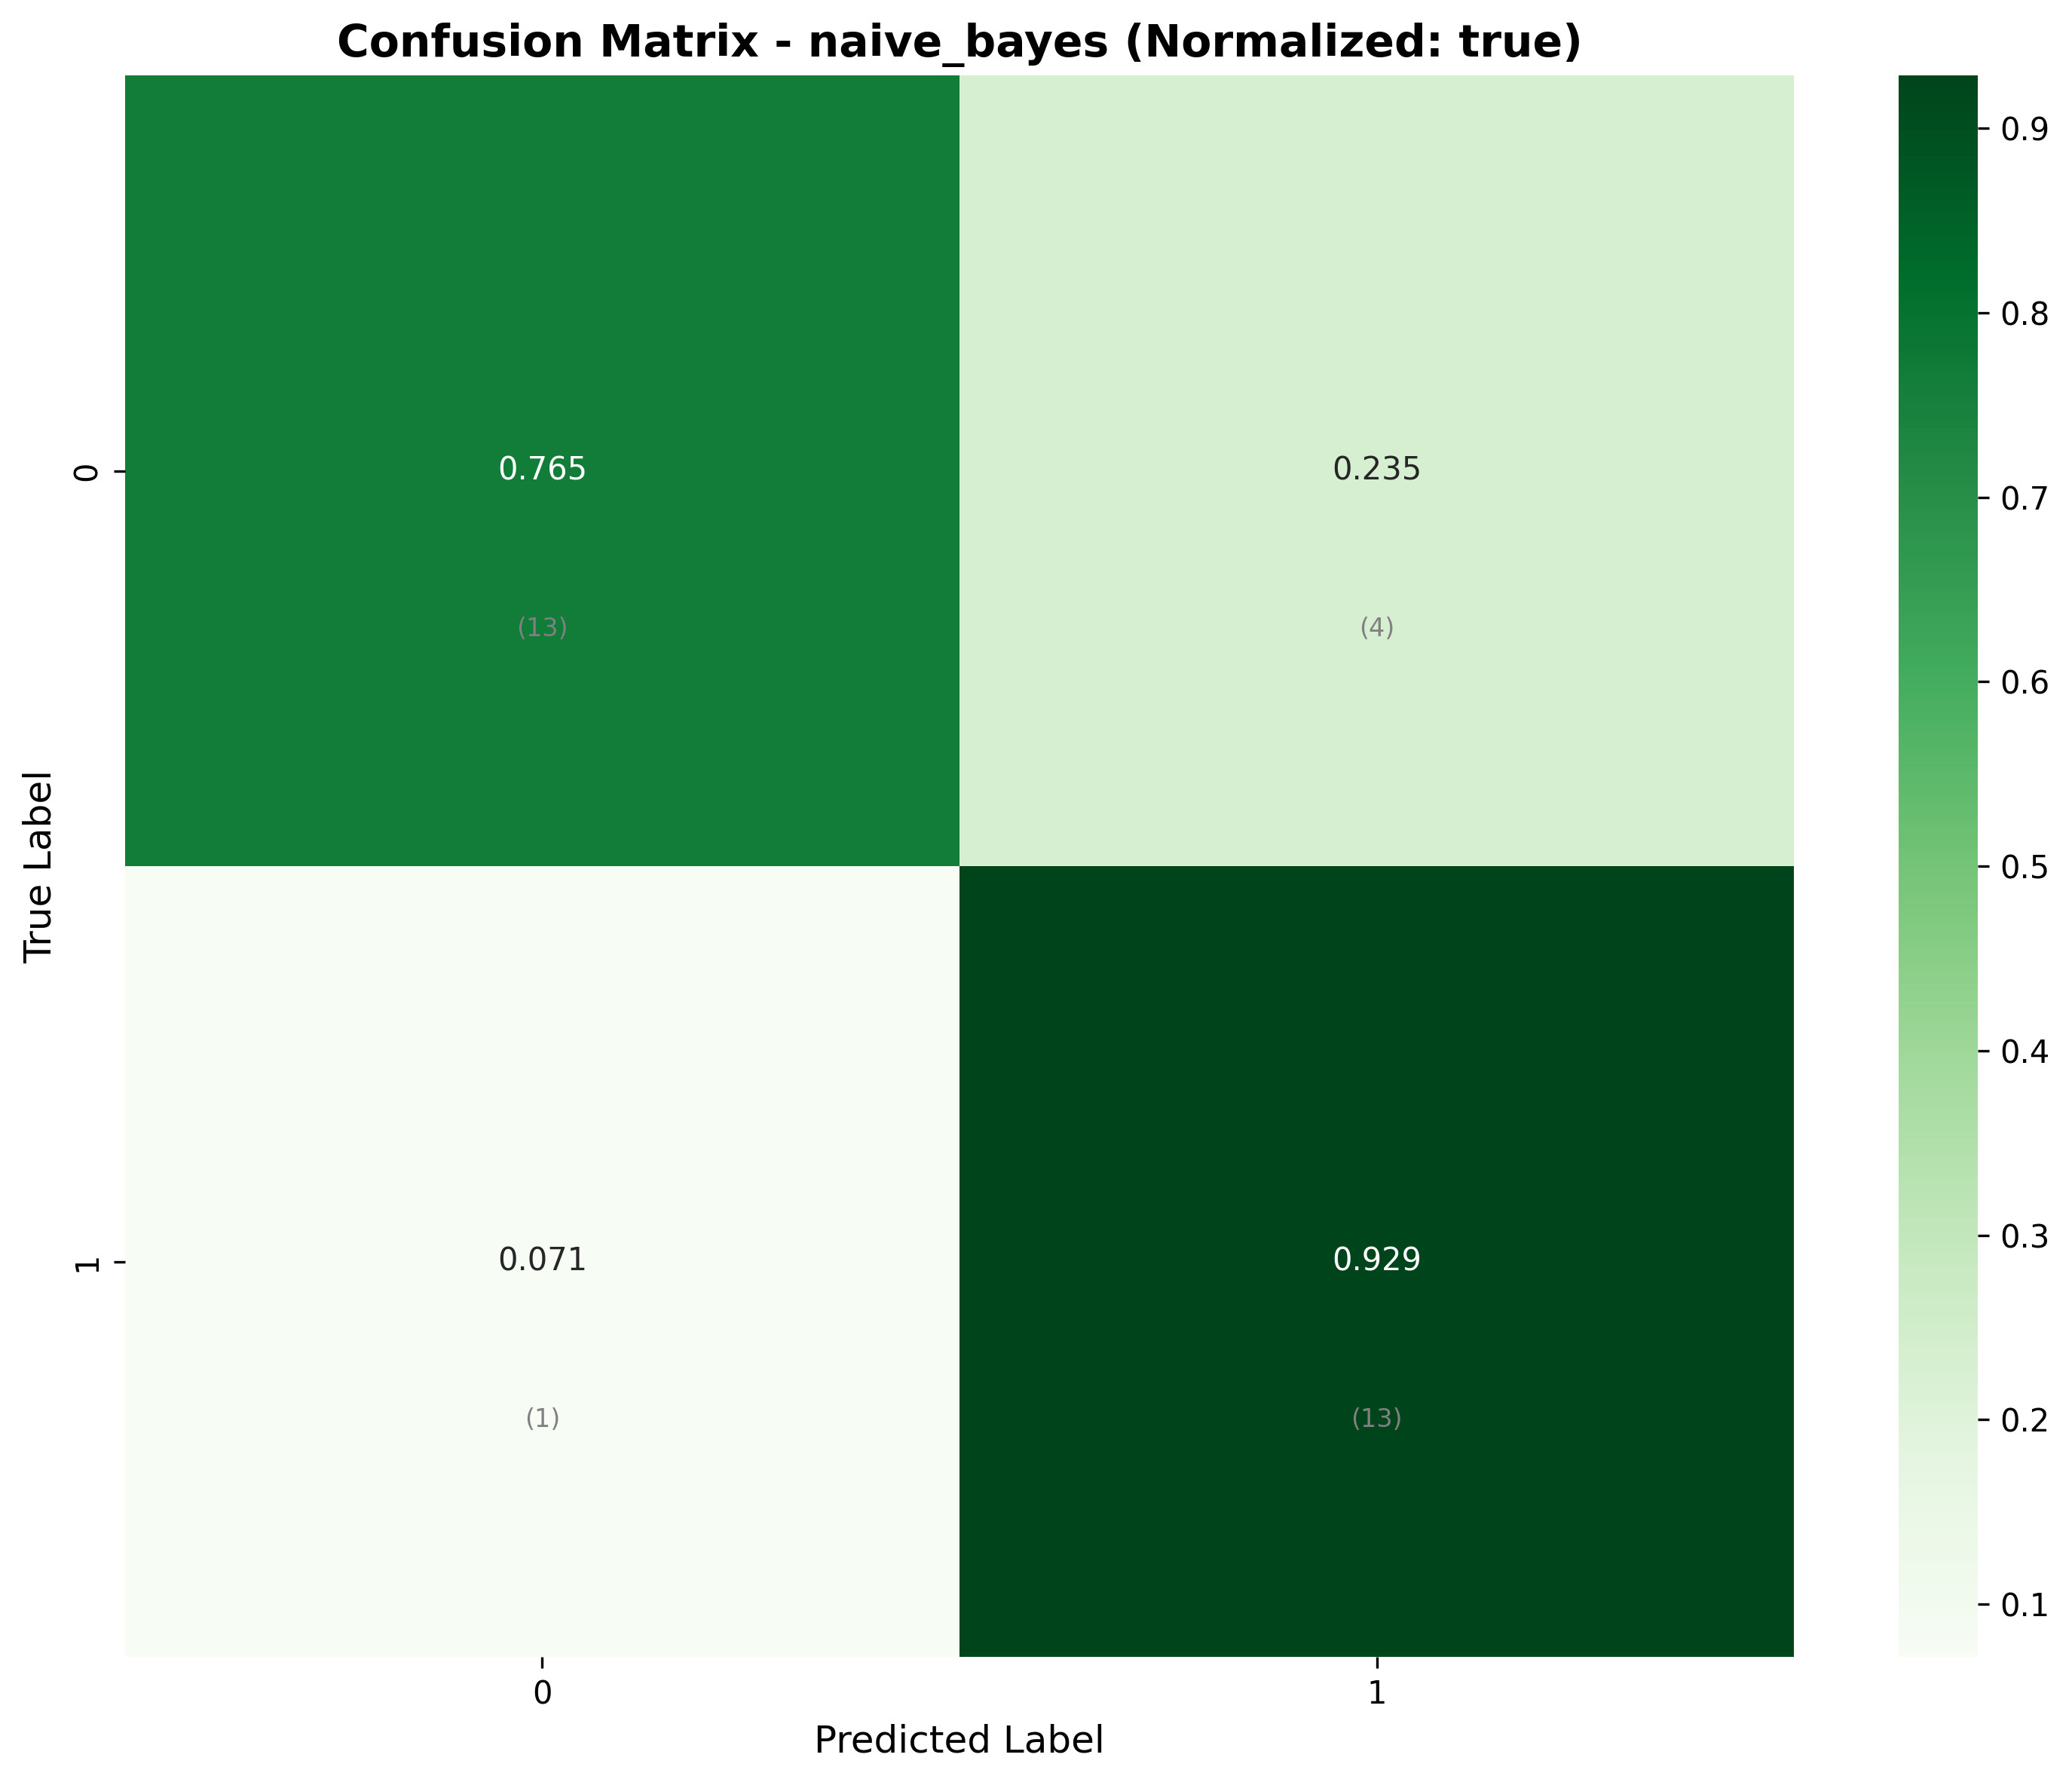
\includegraphics[width=0.95\textwidth]{Result/cleveland_dataset/confusion_matrices/naive_bayes_numeric_dataset_RobustScaler.png}
\caption{NB RobustScaler Consistency}
\label{fig:nb_robust_performance}
\end{subfigure}
\caption{Phương pháp Xác suất Naive Bayes: Huấn luyện siêu nhanh với hiệu suất nhất quán}
\label{fig:naive_bayes_complete}
\end{figure}

Hình \ref{fig:knn_analysis_complete} và \ref{fig:naive_bayes_complete} chứng minh sức mạnh của ML cổ điển: clustering dựa trên khoảng cách và lập luận xác suất với các ưu điểm lâm sàng cụ thể.

\paragraph{AdaBoost và Ensemble Methods}

\textbf{AdaBoost}: Cleveland (80.6\%) với các mẫu học yếu tuần tự và nhấn mạnh đặc trưng dựa trên lỗi. AdaBoost chứng minh cải thiện lặp lại của ranh giới quyết định thông qua việc nhấn mạnh liên tục trên các trường hợp bị phân loại sai, tạo ra ranh giới dự đoán cuối cùng mạnh mẽ với độ phức tạp tính toán vừa phải.

\begin{figure}[H]
\centering
\begin{subfigure}[b]{0.31\textwidth}
\centering
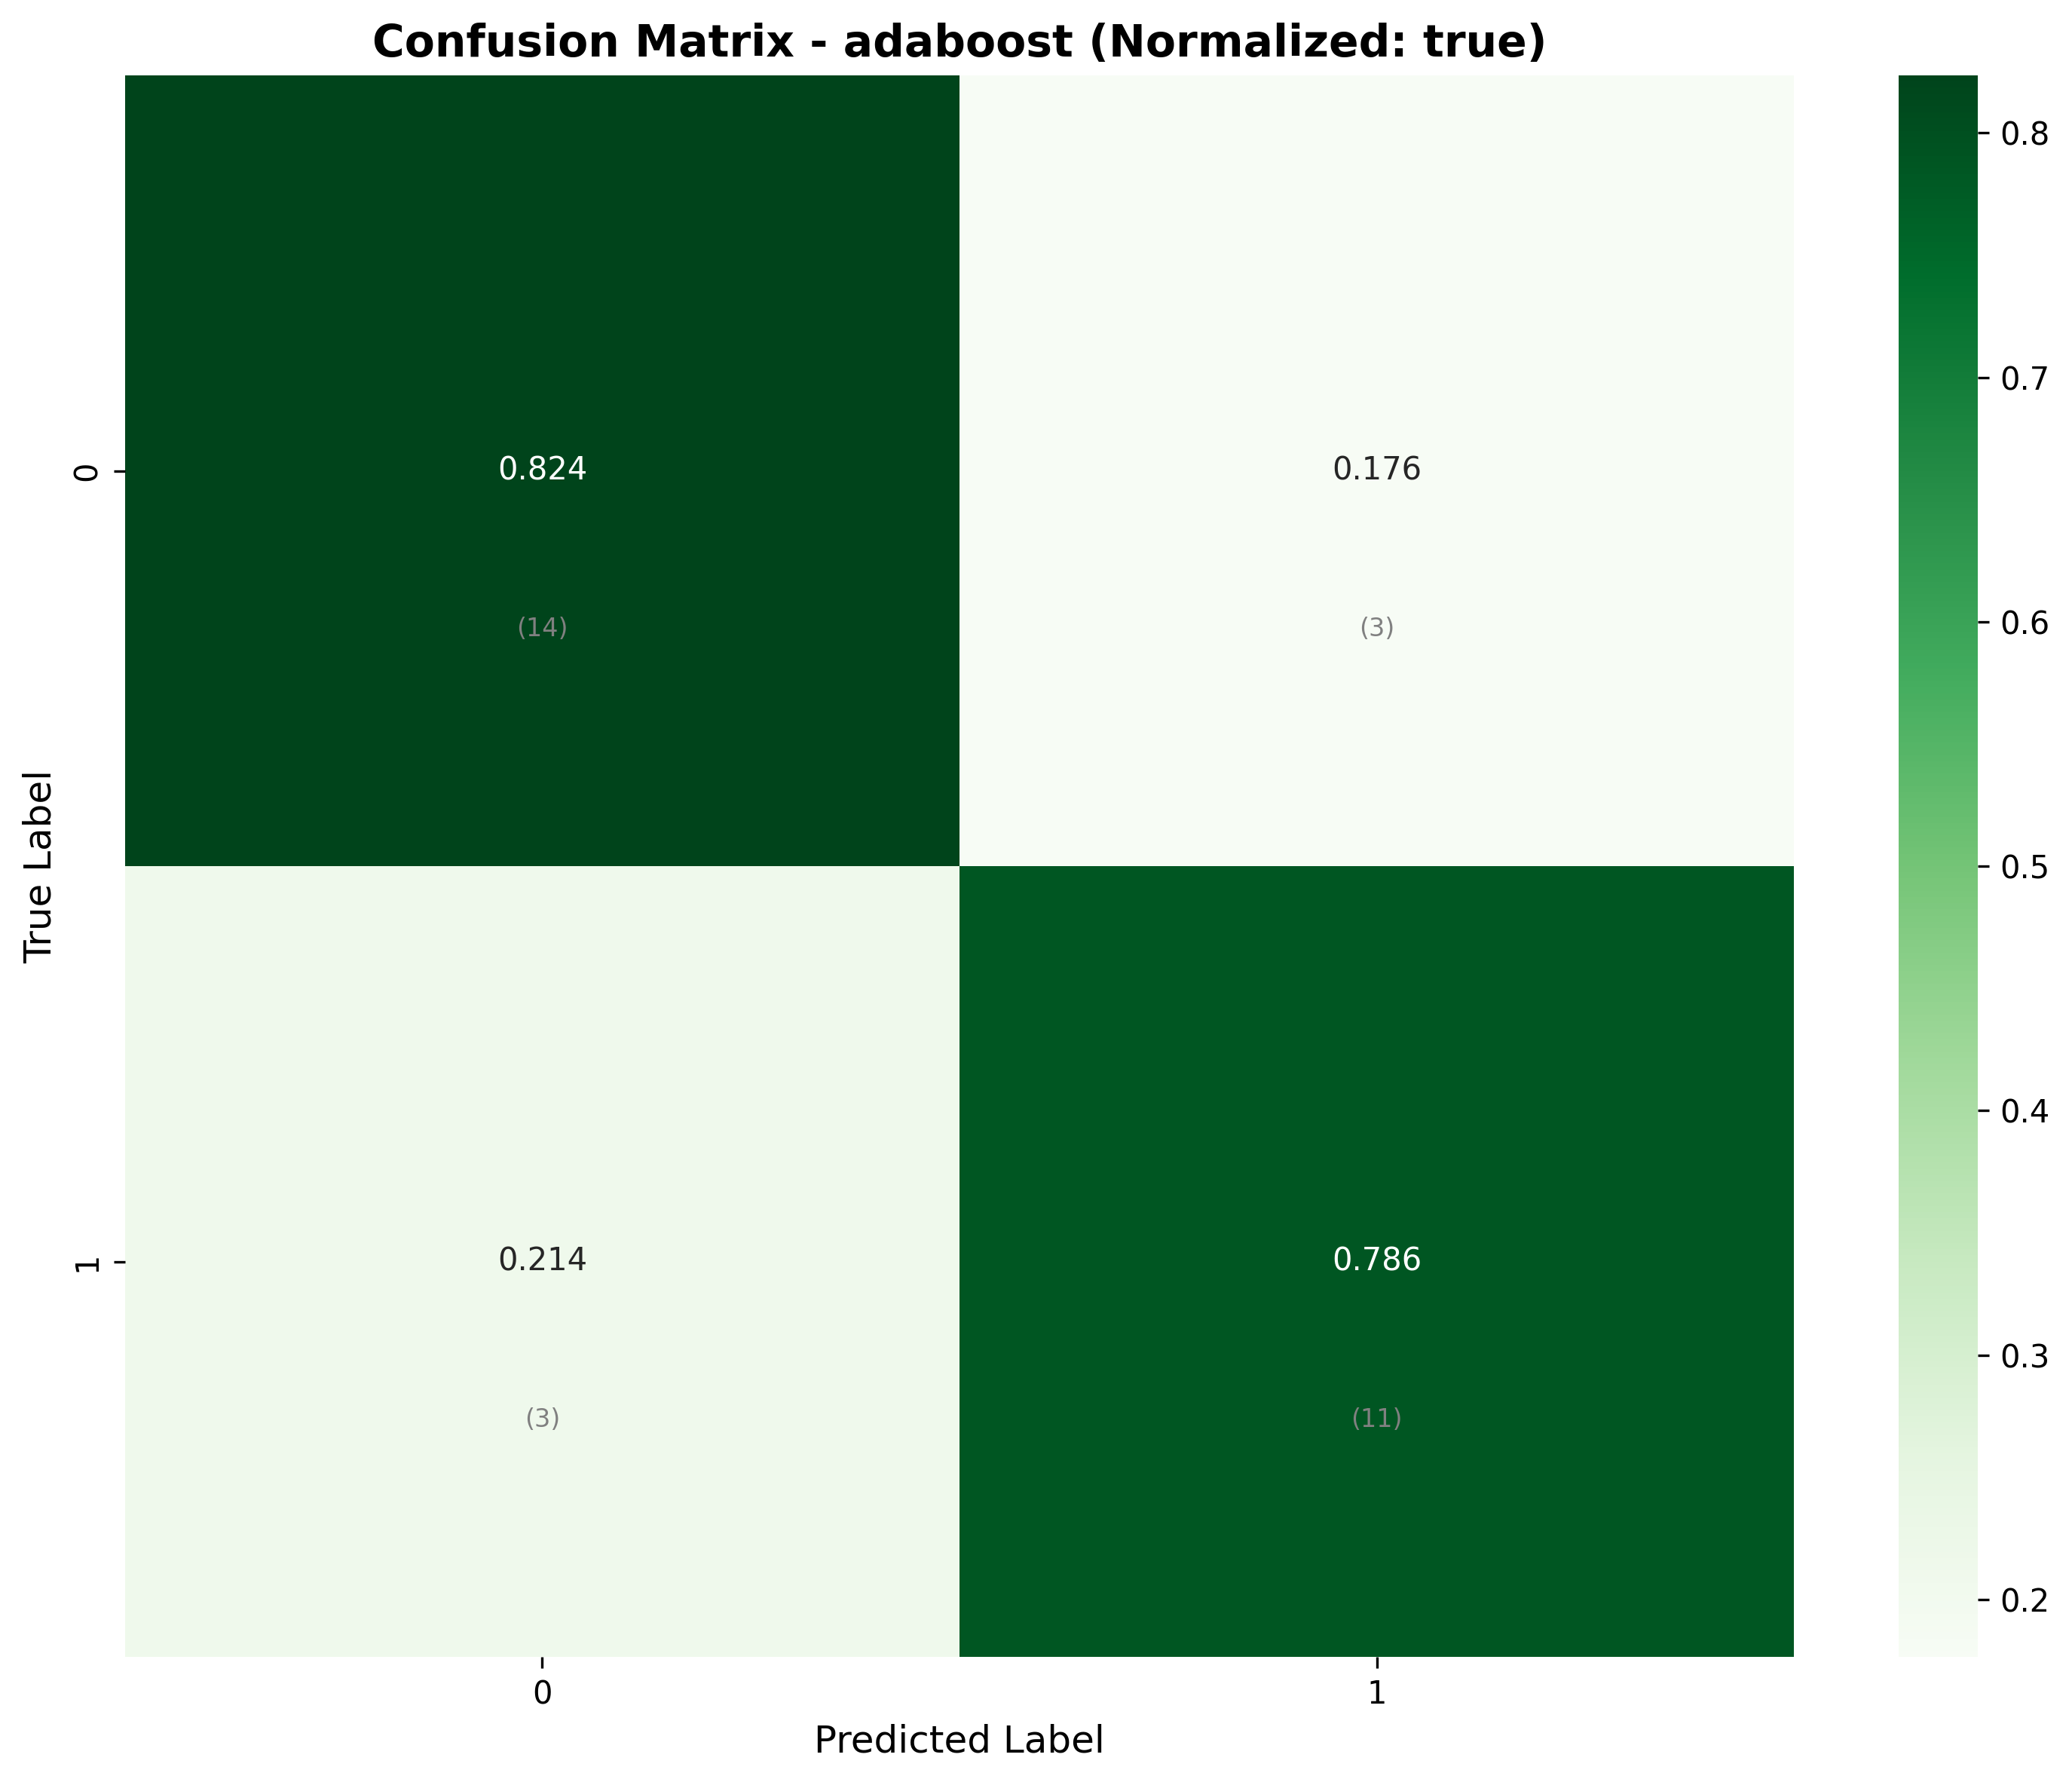
\includegraphics[width=0.95\textwidth]{Result/cleveland_dataset/confusion_matrices/adaboost_numeric_dataset_StandardScaler.png}
\caption{AdaBoost Cleveland (80.6\%)}
\label{fig:ada_cleveland_performance}
\end{subfigure}
\hfill
\begin{subfigure}[b]{0.31\textwidth}
\centering
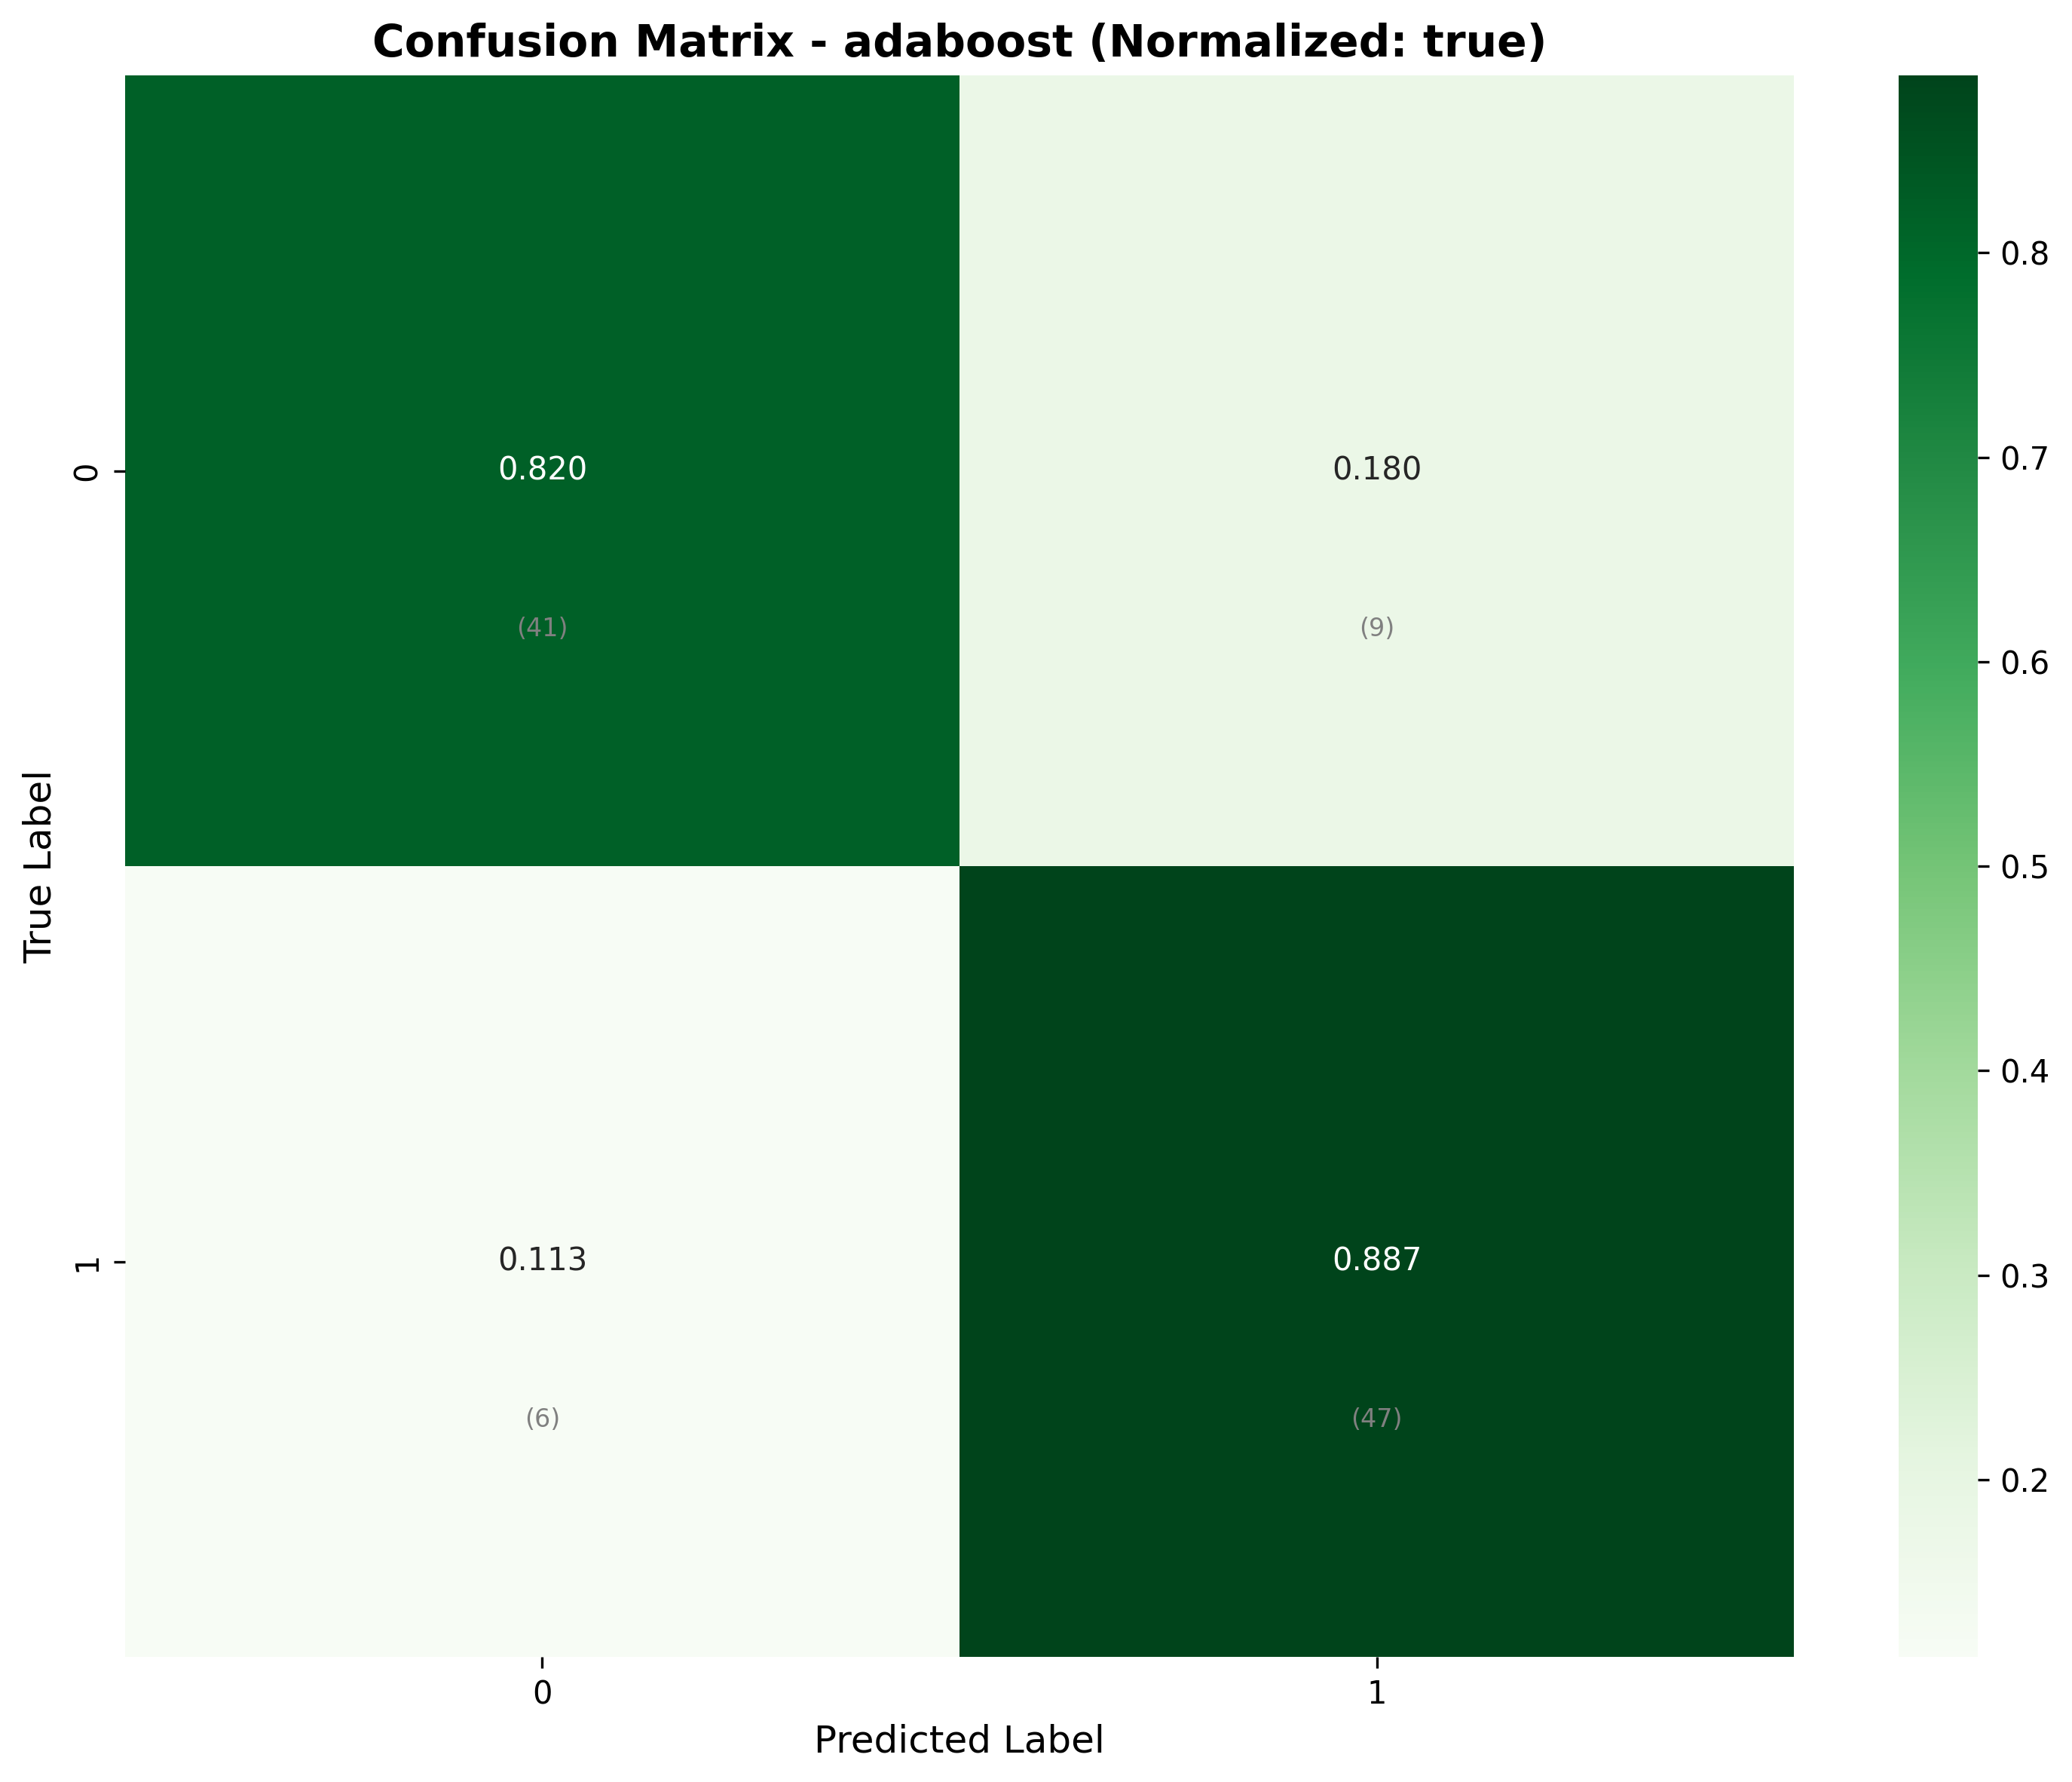
\includegraphics[width=0.95\textwidth]{Result/heart_dataset/confusion_matrices/adaboost_numeric_dataset_StandardScaler.png}
\caption{AdaBoost Heart Dataset}
\label{fig:ada_heart_performance}
\end{subfigure}
\hfill
\begin{subfigure}[b]{0.31\textwidth}
\centering
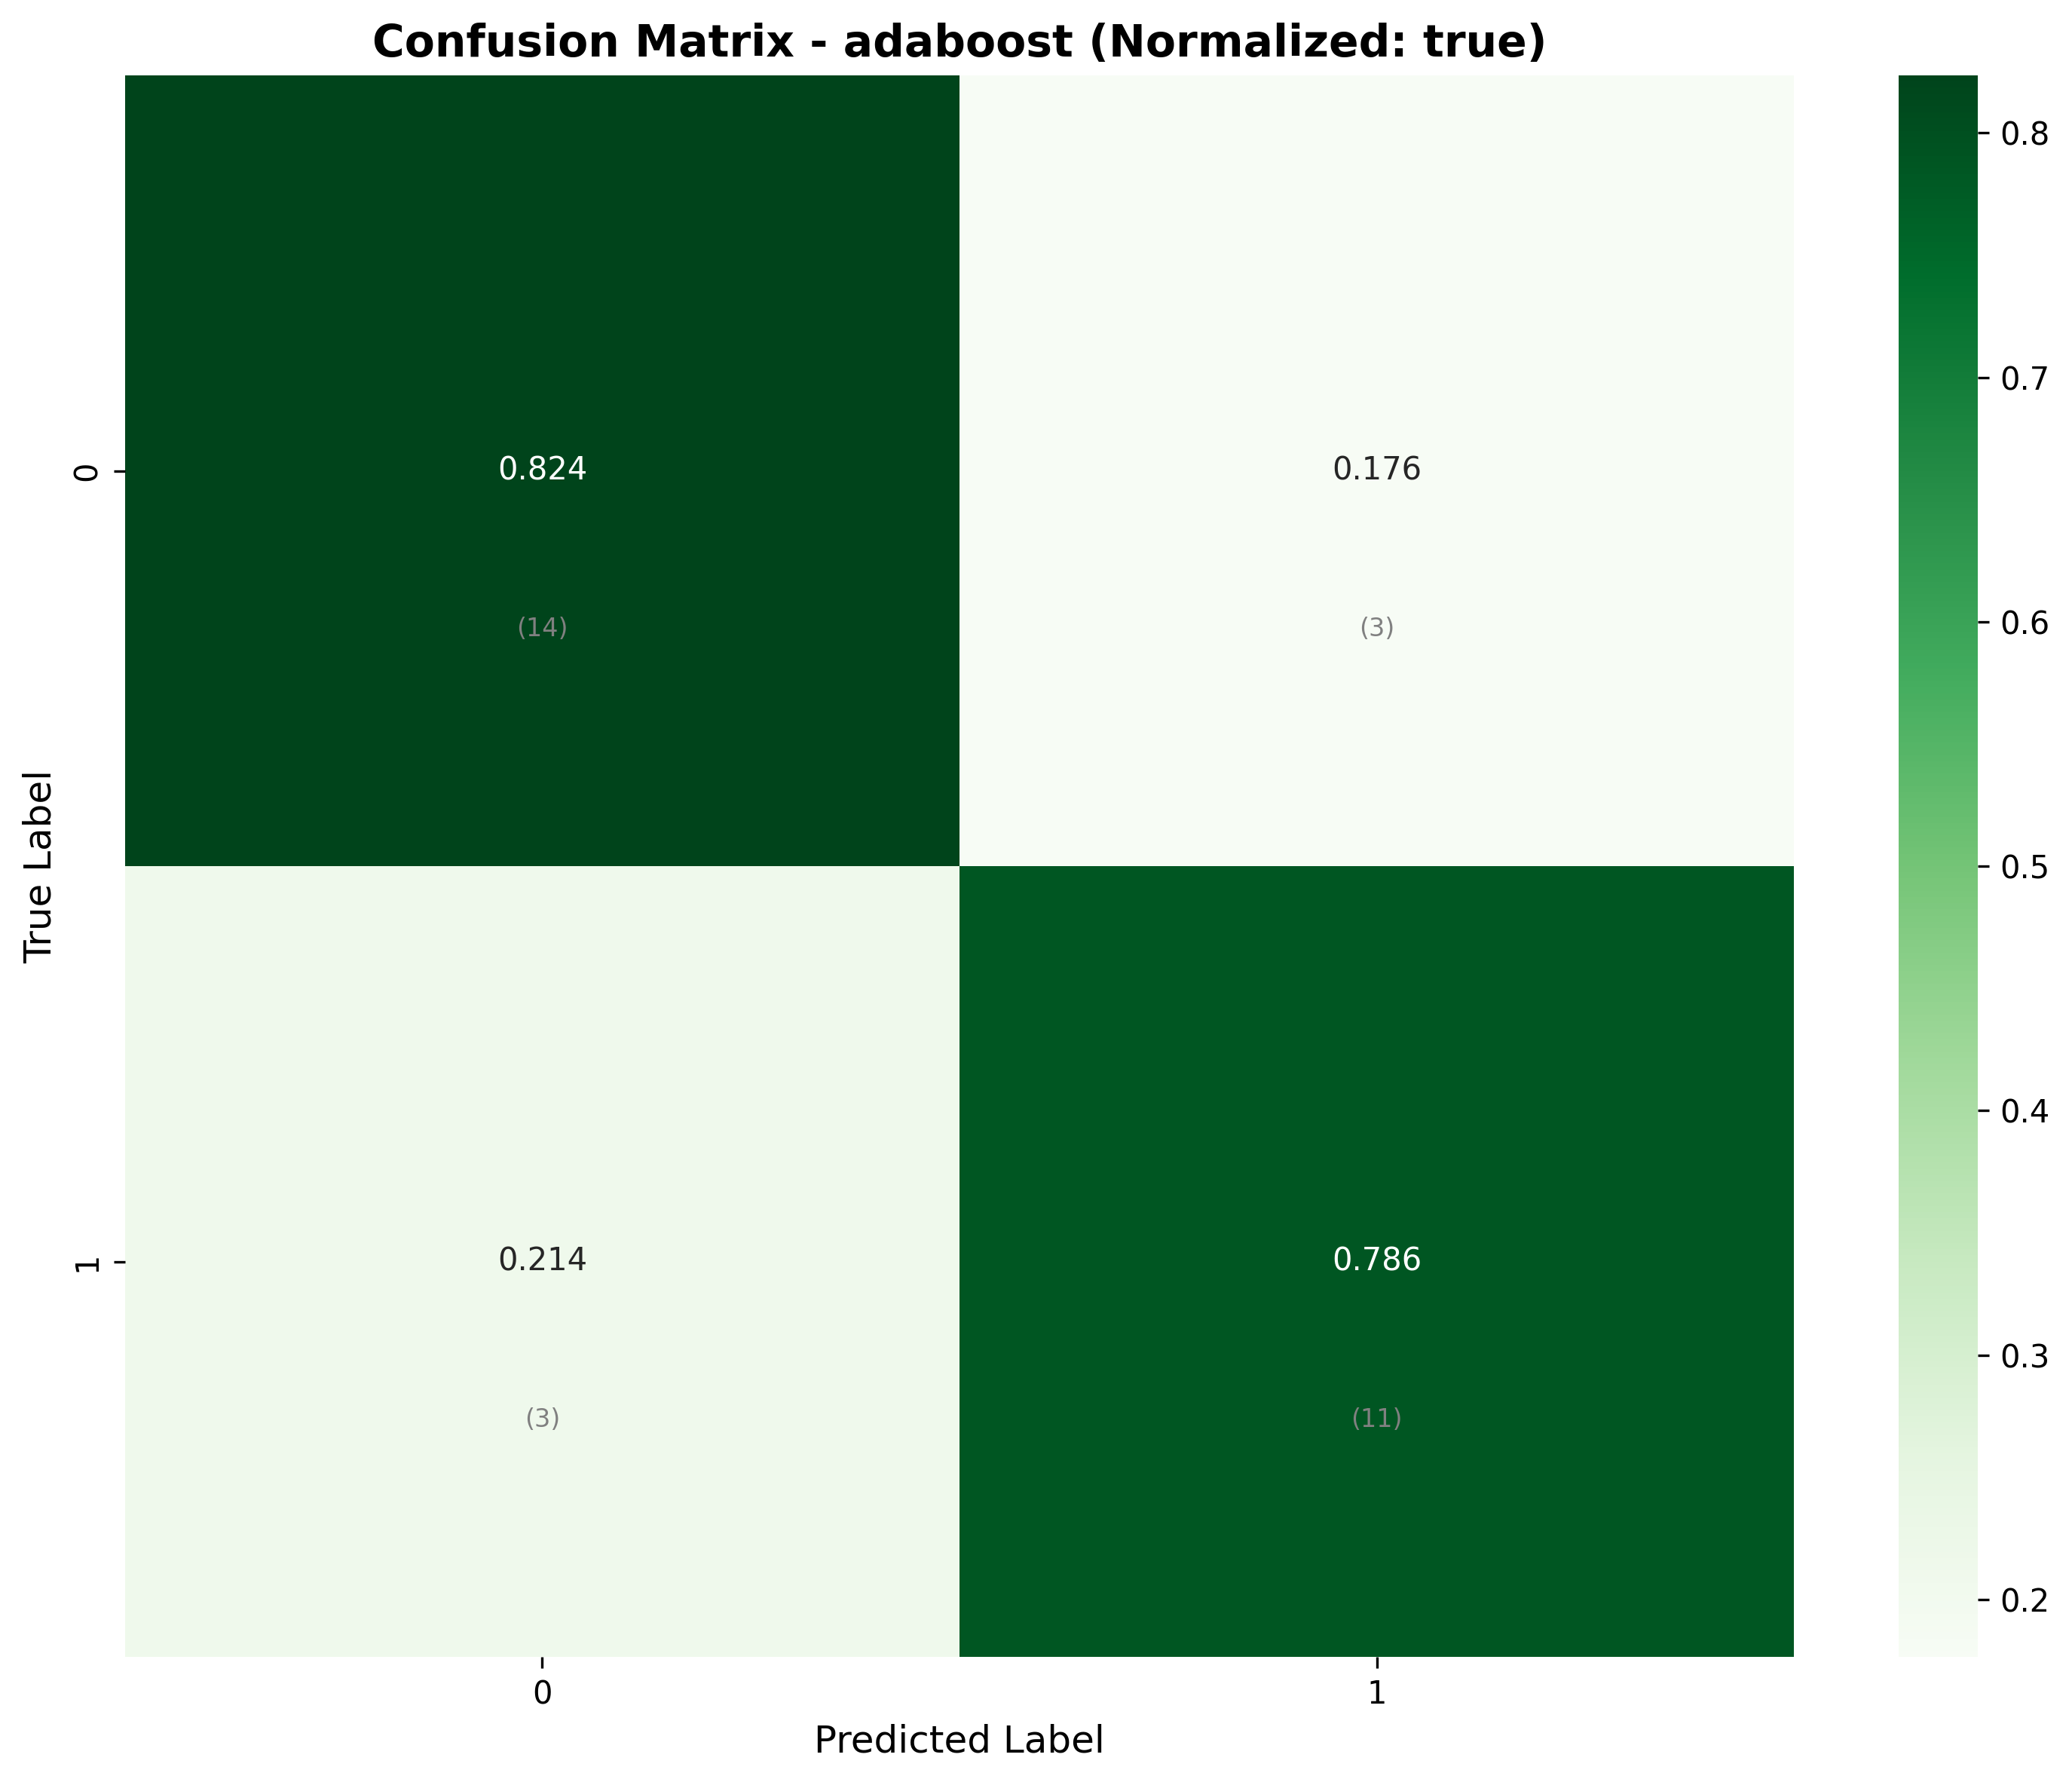
\includegraphics[width=0.95\textwidth]{Result/cleveland_dataset/confusion_matrices/adaboost_numeric_dataset_RobustScaler.png}
\caption{AdaBoost Robust Adaptation}
\label{fig:ada_robust_performance}
\end{subfigure}
\caption{AdaBoost Sequential Learning: Error-driven improvement với adaptive weak learner focus}
\label{fig:adaboost_analysis_complete}
\end{figure}

\textbf{Voting Ensemble (Hard)}: Cleveland (83.9-87.1\%) → Heart (96.1-98.1\%). Hard voting đạt được độ chính xác cao qua consensus đa số với implementation đơn giản và training nhanh (5.92-6.34 giây), hạn chế đến discrete prediction combinations mà không khai thác continuous probability distributions.

\begin{figure}[H]
\centering
\begin{subfigure}[b]{0.48\textwidth}
\centering
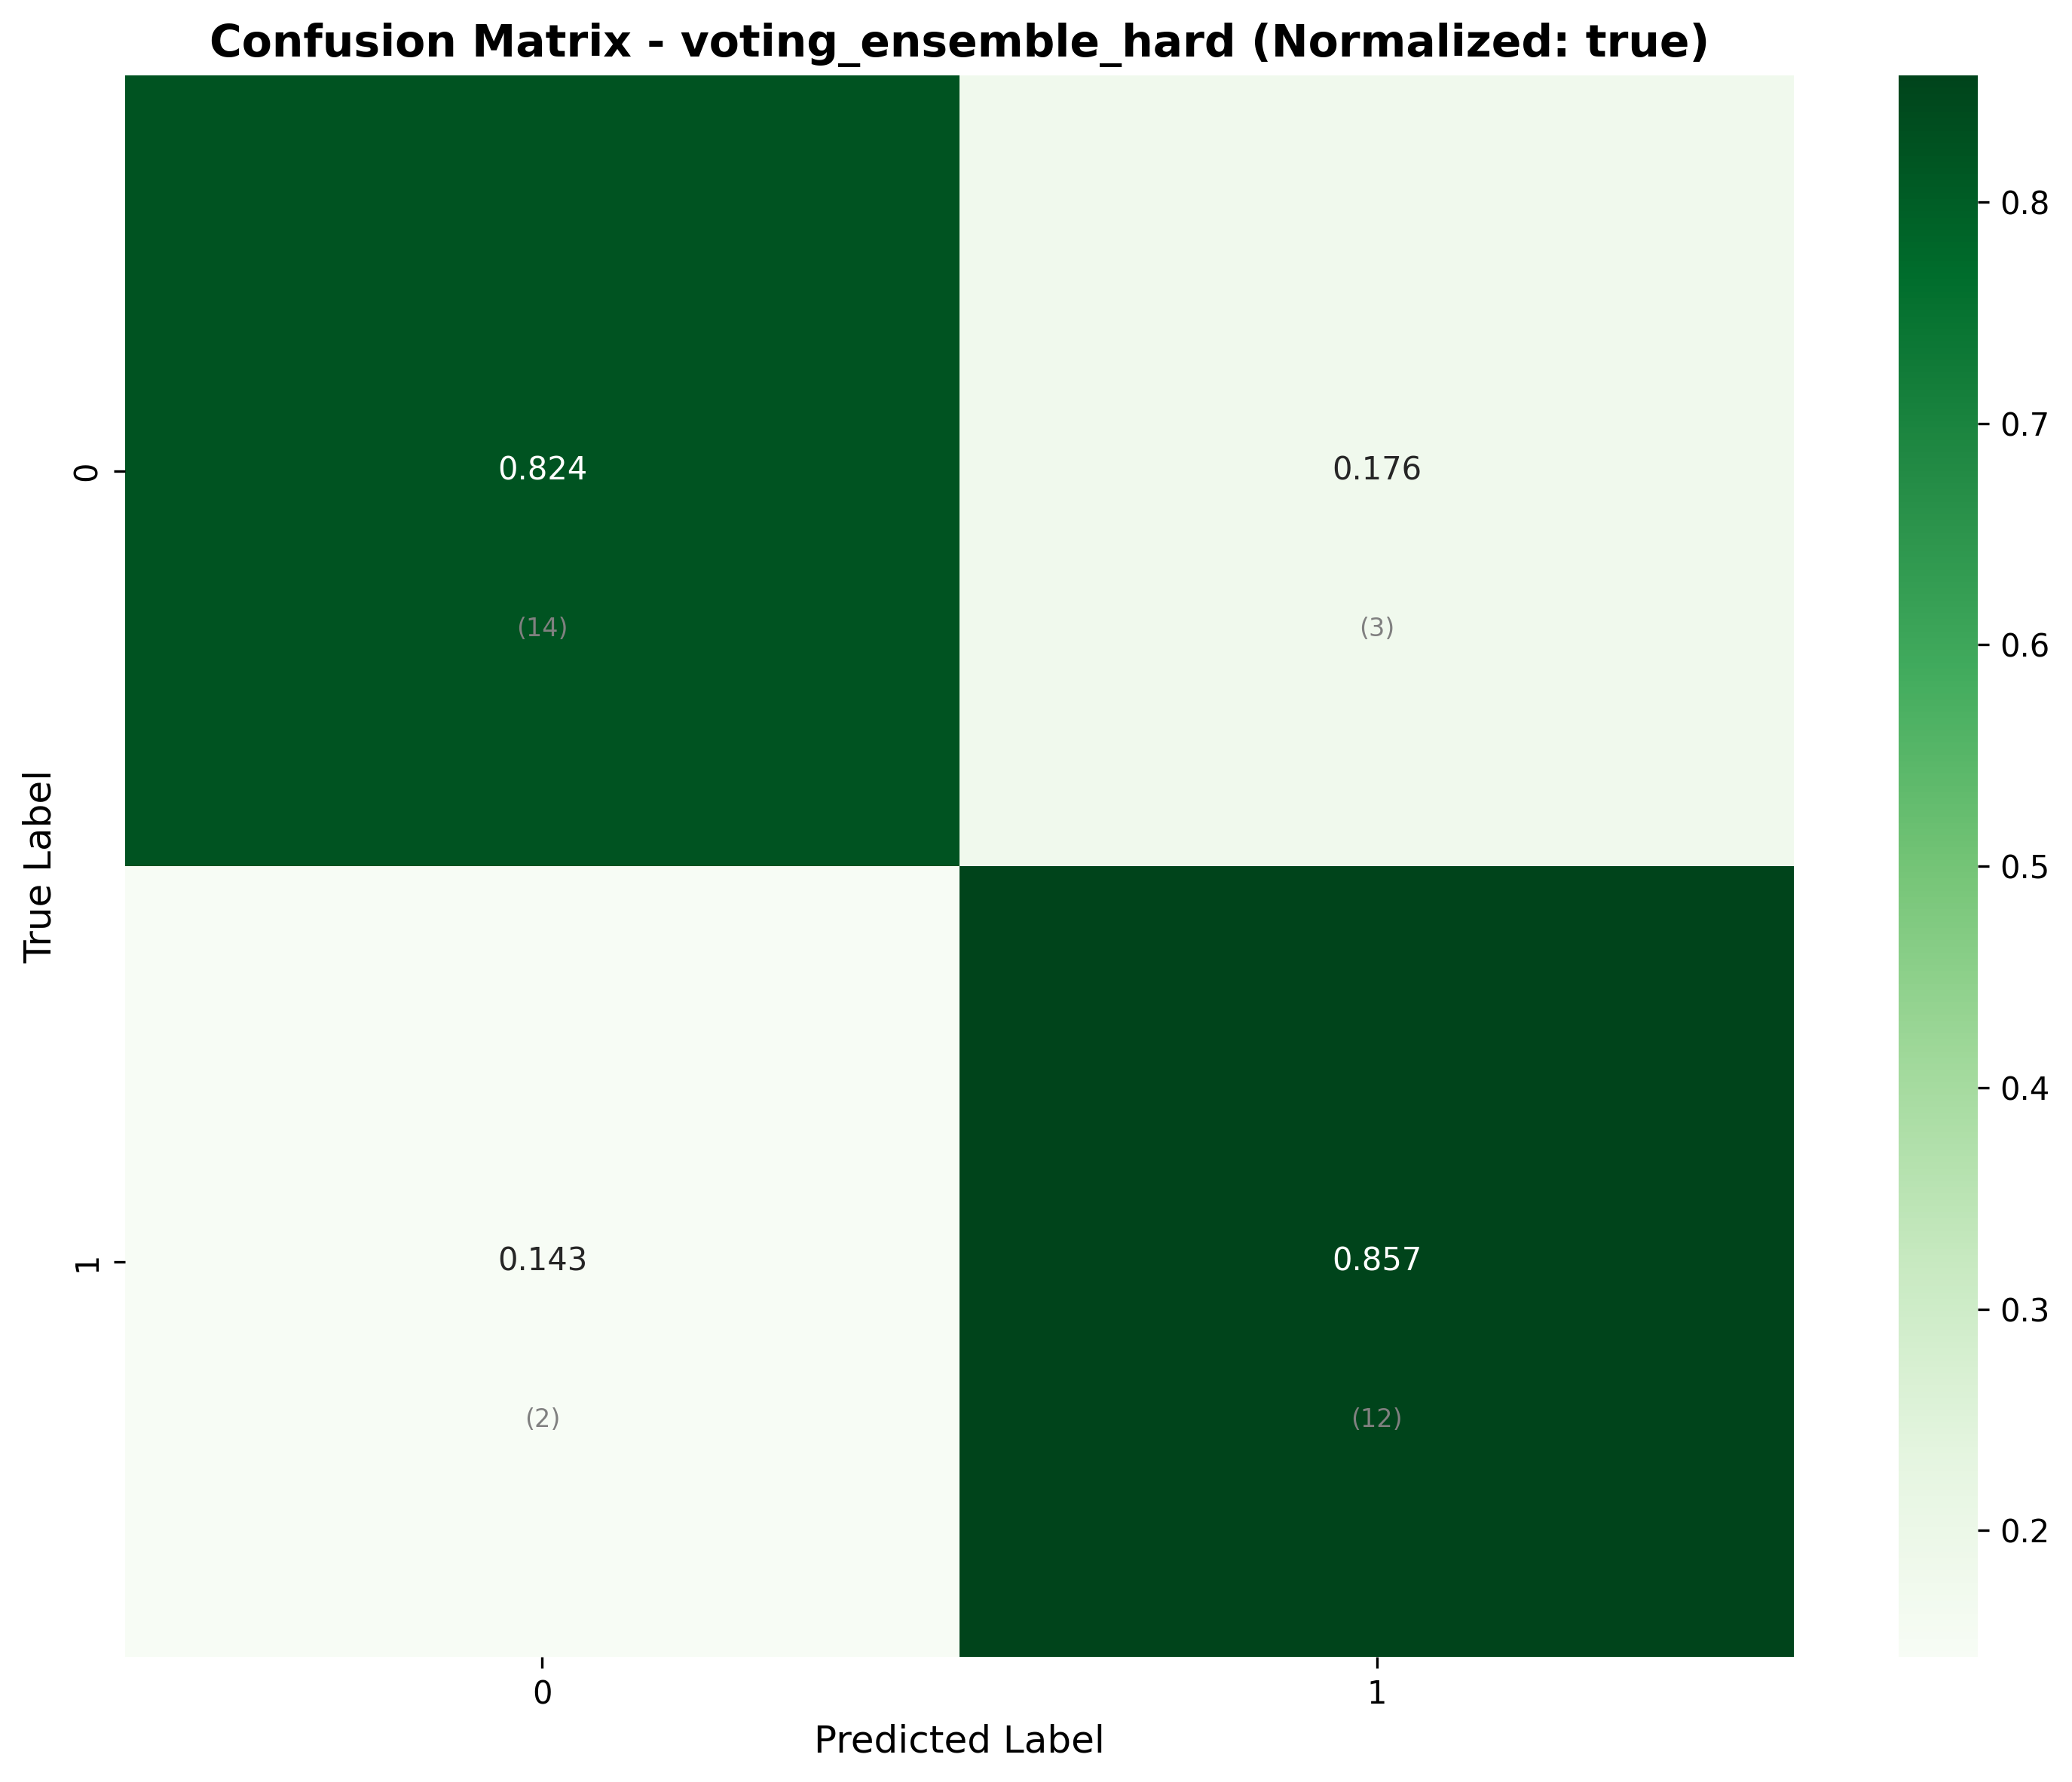
\includegraphics[width=0.95\textwidth]{Result/cleveland_dataset/confusion_matrices/voting_ensemble_hard_numeric_dataset_StandardScaler.png}
\caption{Voting Cleveland (83.9-87.1\%)}
\label{fig:voting_cleveland_performance}
\end{subfigure}
\hfill
\begin{subfigure}[b]{0.48\textwidth}
\centering
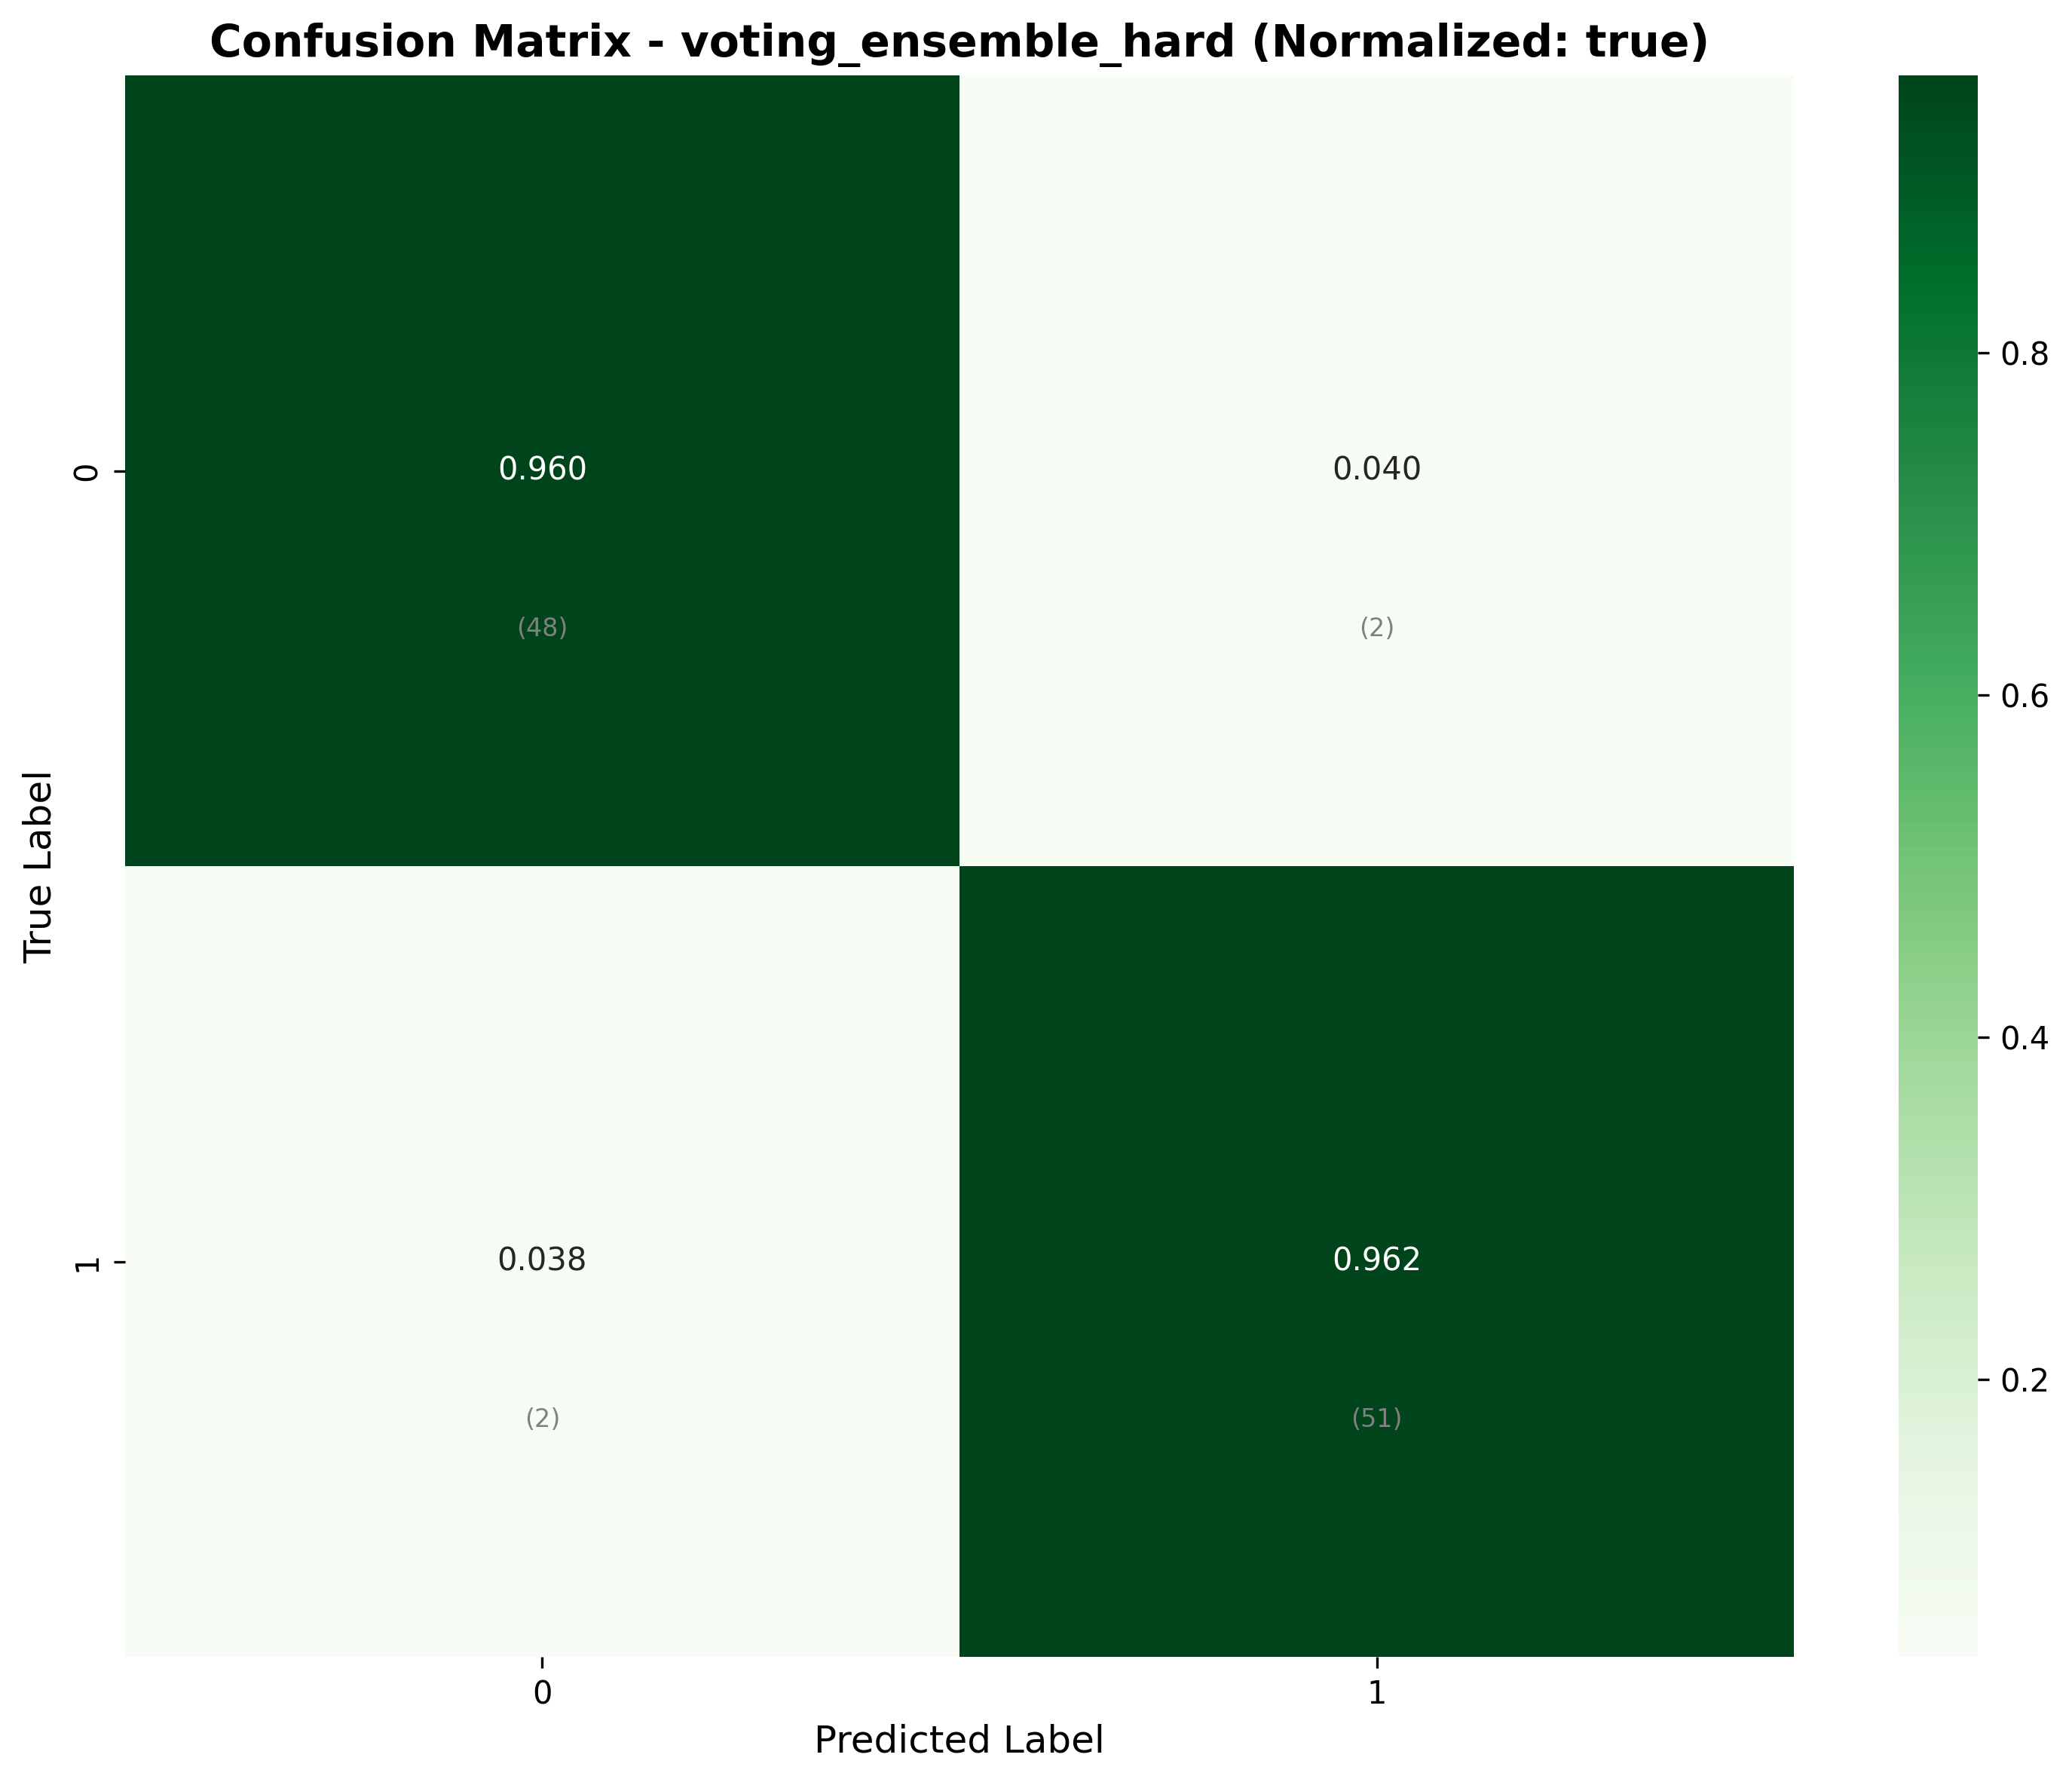
\includegraphics[width=0.95\textwidth]{Result/heart_dataset/confusion_matrices/voting_ensemble_hard_numeric_dataset_StandardScaler.png}
\caption{Voting Heart (96.1-98.1\%)}
\label{fig:voting_heart_performance}
\end{subfigure}
\caption{Voting Ensemble Democratic Approach: Multiple algorithm consensus cho robust predictions}
\label{fig:voting_analysis_complete}


\end{figure}

\textbf{Stacking Ensemble}: Cleveland (87.1\%) → Heart (100\% với Logistic Regression meta-learner). Stacking với meta-learner đạt được hiệu suất vượt trội qua học cách tối ưu linear combination weights của base model predictions, tạo learned voting strategy thích ứng đến dataset-specific patterns với moderate computational overhead (22.8-23.8 giây).

\begin{figure}[H]
\centering
\begin{subfigure}[b]{0.48\textwidth}
\centering
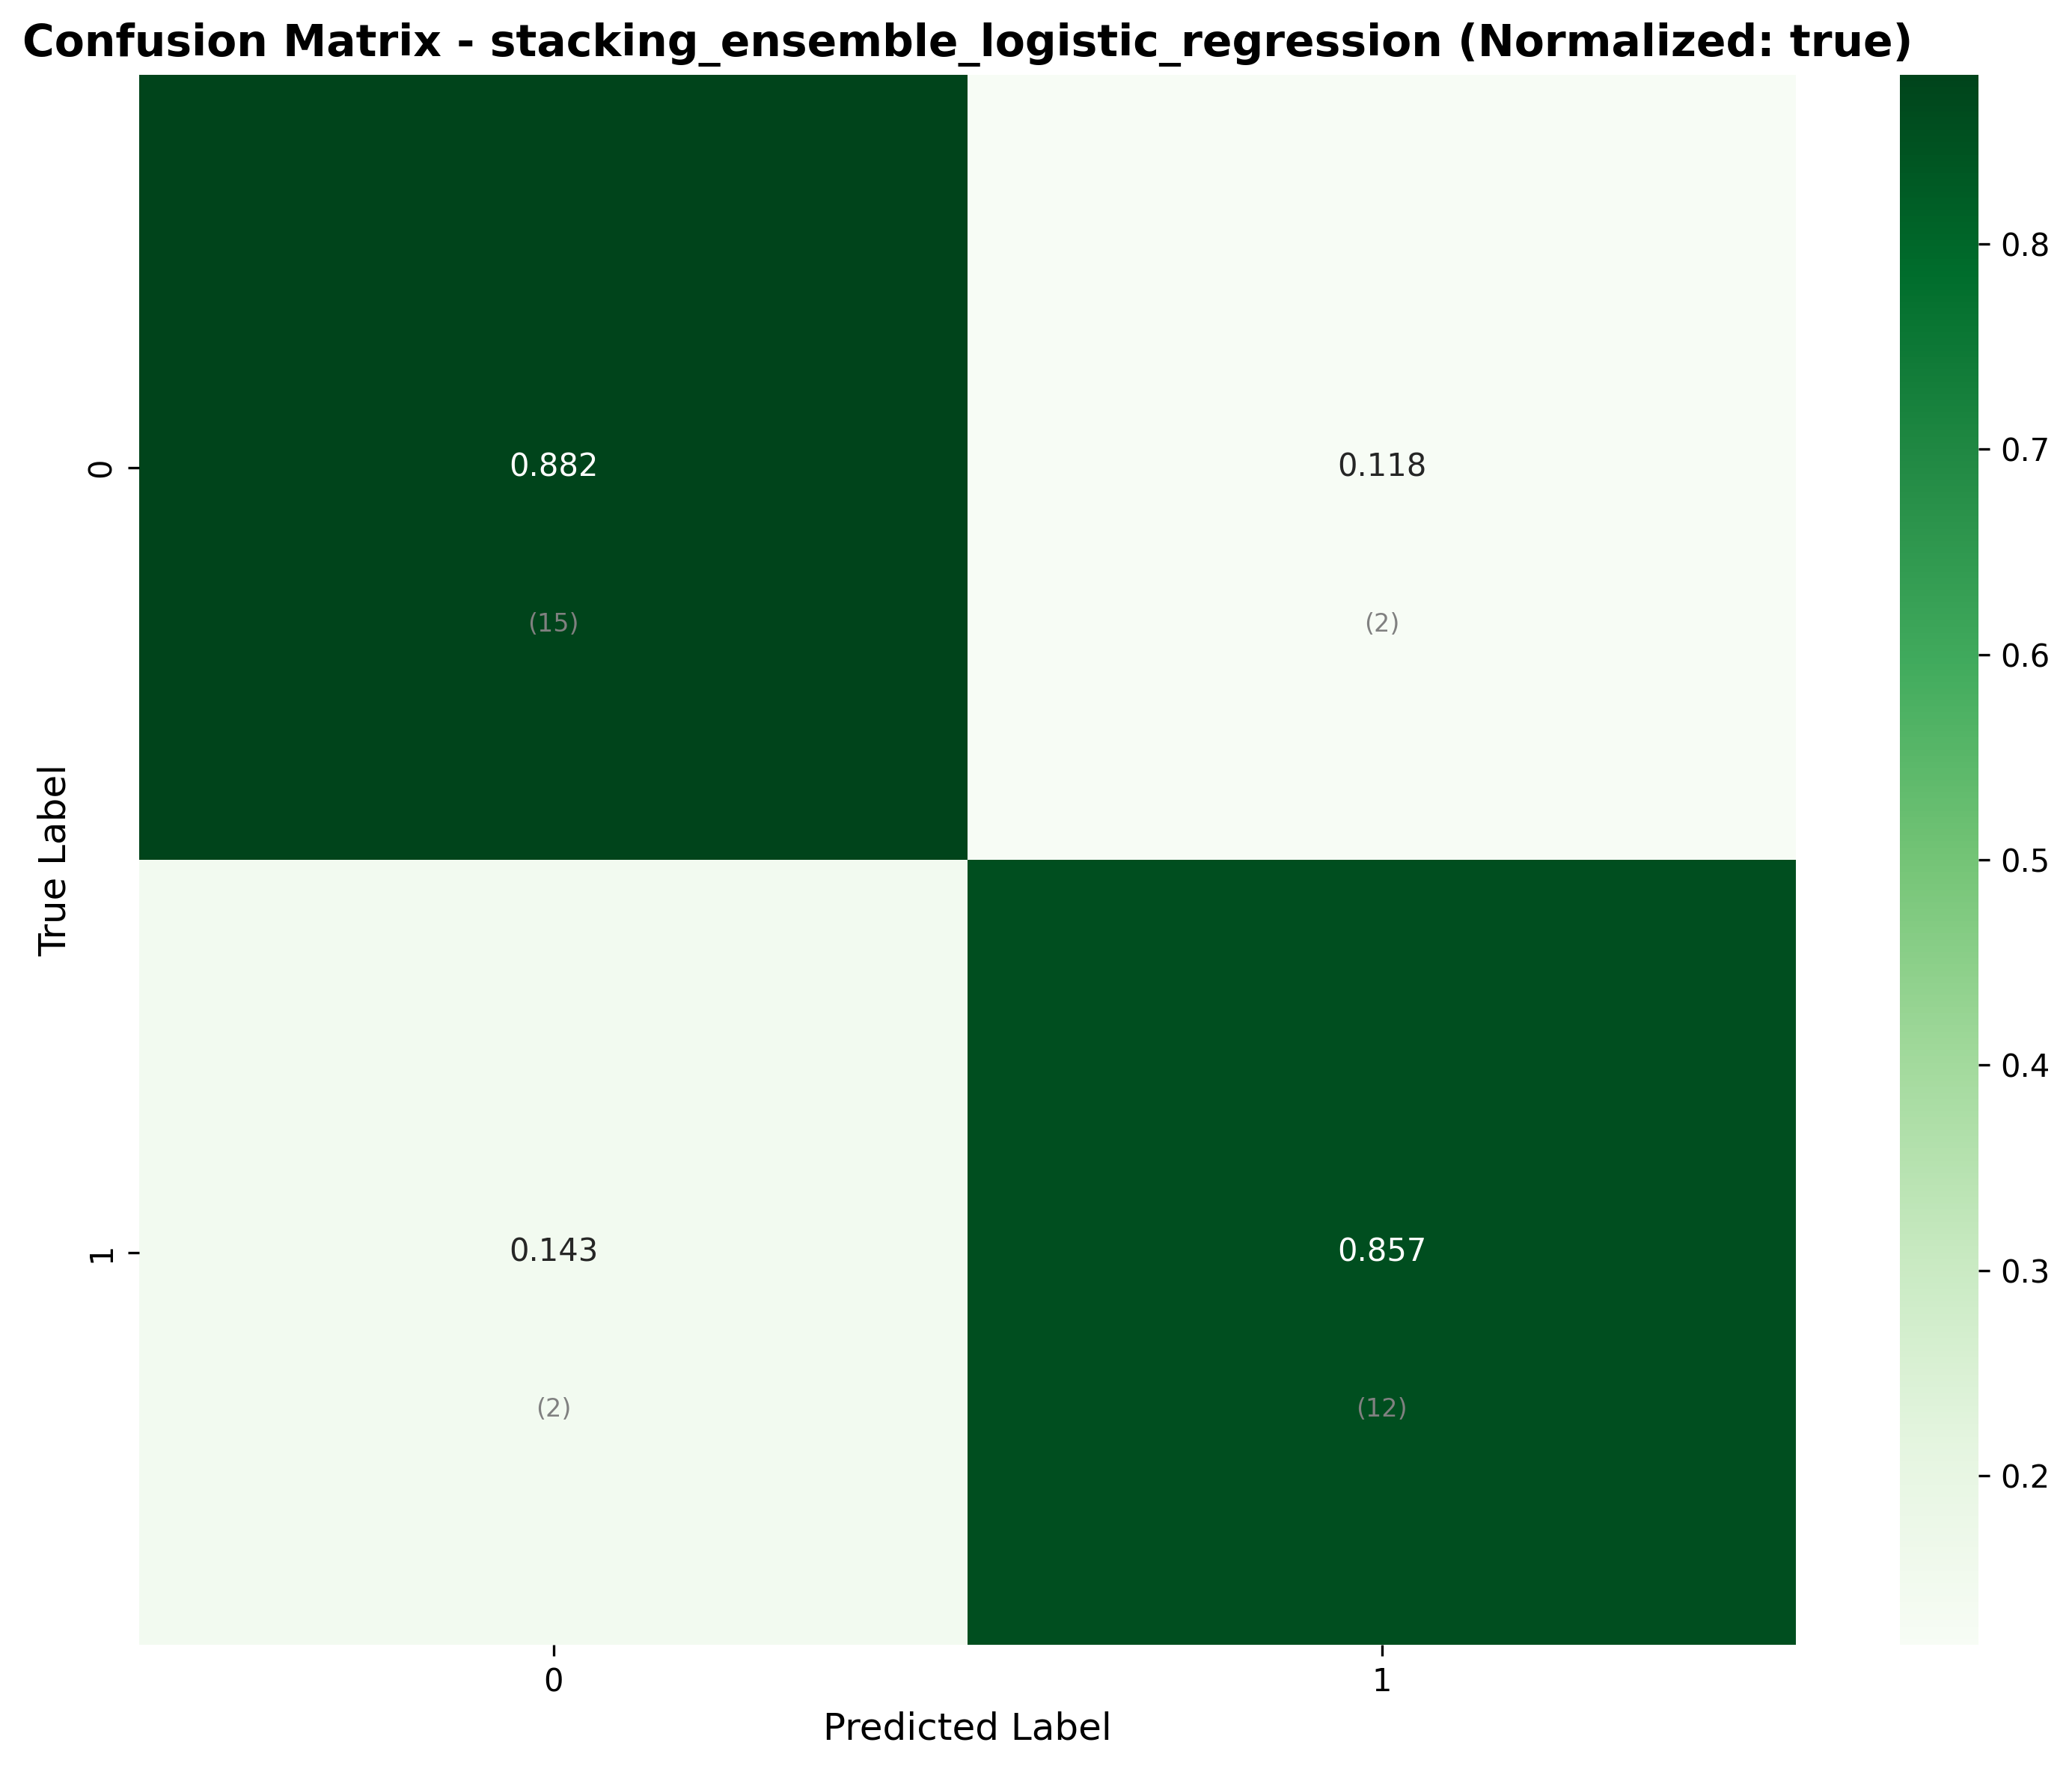
\includegraphics[width=0.95\textwidth]{Result/cleveland_dataset/confusion_matrices/stacking_ensemble_logistic_regression_numeric_dataset_StandardScaler.png}
\caption{Stacking Cleveland (87.1\%)}
\label{fig:stacking_cleveland_performance}
\end{subfigure}
\hfill
\begin{subfigure}[b]{0.48\textwidth}
\centering
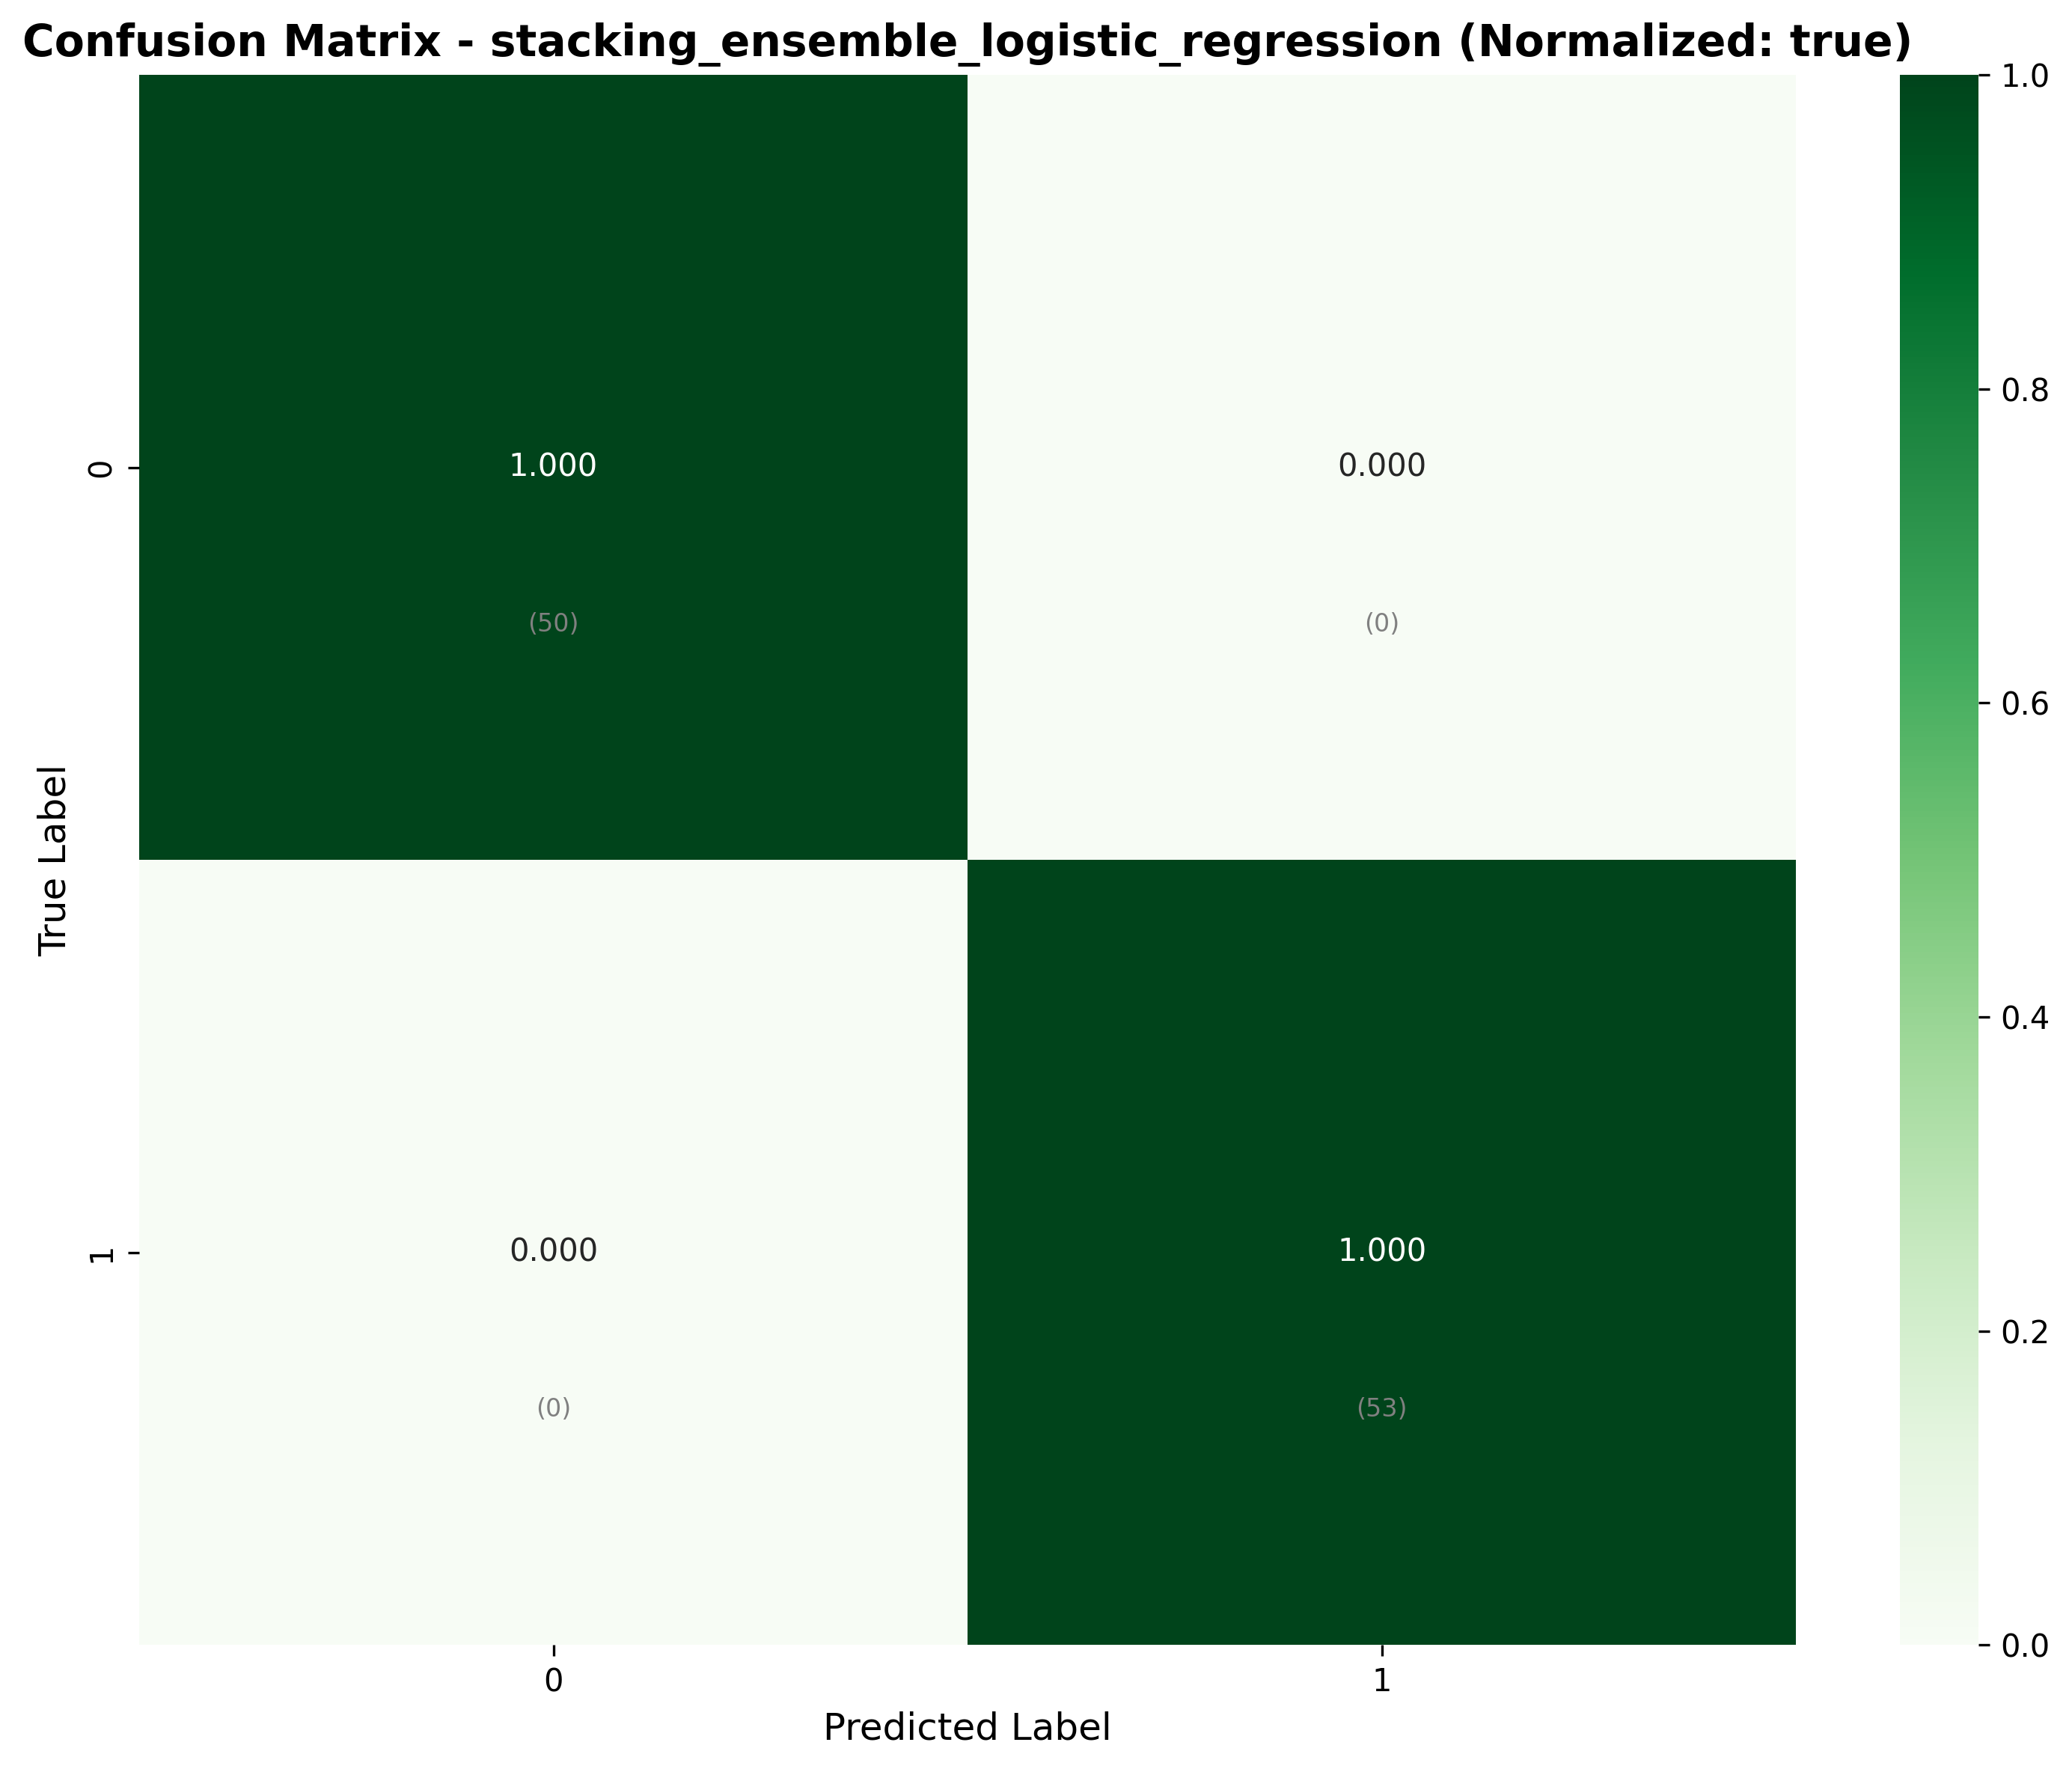
\includegraphics[width=0.95\textwidth]{Result/heart_dataset/confusion_matrices/stacking_ensemble_logistic_regression_numeric_dataset_StandardScaler.png}
\caption{Stacking Heart (100\%)}
\label{fig:stacking_heart_performance}
\end{subfigure}
\caption{Stacking Meta-Learning: Optimal algorithm combination với adaptive prediction synthesis}
\label{fig:stacking_analysis_complete}
\end{figure}

Các Hình \ref{fig:adaboost_analysis_complete}, \ref{fig:voting_analysis_complete} và \ref{fig:stacking_analysis_complete} thể hiện các chiến lược ensemble khác nhau: sequential learning, democratic voting, và meta-learning approaches với ứng dụng lâm sàng khác biệt.

\subsubsection{Các Hiểu biết Chủ chốt từ So sánh Cross-Dataset}

\textbf{Tác động Kích cỡ Dataset}: Heart Dataset (1025 samples) cho phép models học được patterns đa dạng hơn từ multiple hospital centers → hiệu suất được cải thiện chung trên most algorithms.

\textbf{Tác động Missing Values}: CatBoost xử lý missing values tốt hơn Random Forest trên Heart Dataset với automatic categorical encoding và ordered boosting giảm target leakage.

\textbf{Hệ thống phân cấp Scaler Sensitivity}:
\begin{itemize}
    \item \textbf{Robust với Scalers}: Random Forest, CatBoost, Naive Bayes
    \item \textbf{Moderate Sensitivity}: Logistic Regression, Gradient Boosting  
    \item \textbf{High Sensitivity}: SVM, KNN, AdaBoost
\end{itemize}

\textbf{Feature Handling Capabilities}:
\begin{itemize}
    \item \textbf{Categorical Features}: CatBoost > Random Forest > Decision Tree
    \item \textbf{Continuous Features}: SVM > Logistic Regression > Naive Bayes
    \item \textbf{Mixed Features}: Random Forest > XGBoost > LightGBM
\end{itemize}

\subsection{Phân tích Tầm quan trọng Đặc trưng từ SHAP}\label{subsec:ra-feature-importance-analysis}

Dựa trên phân tích SHAP toàn diện của 39 cấu hình mô hình trên Cleveland Dataset và Heart Dataset, phần này trình bày insights về tầm quan trọng đặc trưng theo nhóm mô hình và so sánh các mẫu giữa hai bộ dữ liệu.

\subsubsection{Các Yếu tố Dự báo Lâm sàng Phổ quát}

Từ phân tích SHAP cross-model, các đặc trưng sau thể hiện tầm quan trọng phổ quát qua các thuật toán:

\textbf{Cấp 1: Các Yếu tố Dự báo Hàng đầu (Tầm quan trọng Trung bình > 0.4)}:
\begin{itemize}
    \item \textbf{ca (Chụp X-quang Mạch máu lớn)}: 0.5105 mức độ quan trọng trung bình - Đánh giá hình ảnh X-quang trực tiếp của bệnh động mạch vành
    \item \textbf{thal (Xét nghiệm Thallium Stress)}: 0.4225 mức độ quan trọng trung bình - Kết quả hình ảnh hạt nhân phát hiện các khuyết tật lưu thông máu  
    \item \textbf{cp (Loại Đau ngực)}: 0.4024 mức độ quan trọng trung bình - Biểu hiện triệu chứng chính trong đánh giá tim mạch
\end{itemize}

\textbf{Cấp 2: Các Yếu tố Dự báo Trung bình (Tầm quan trọng Trung bình 0.3-0.4)}:
\begin{itemize}
    \item \textbf{oldpeak (Biến thiên ST)}: 0.3292 mức độ quan trọng trung bình - Thay đổi ECG do tập thể dục cho thấy thiếu máu cơ tim
    \item \textbf{thalach (Nhịp tim Tối đa)}: ~0.32 mức độ quan trọng trung bình - Chỉ số thể lực tim với khoảng 71-202 nhịp/phút
    \item \textbf{age (Thông tin Nhân khẩu học)}: ~0.30 mức độ quan trọng trung bình - Yếu tố rủi ro tim mạch không thể thay đổi (29-77 tuổi)
\end{itemize}

\textbf{Cấp 3: Các Yếu tố Dự báo Thấp (Tầm quan trọng Trung bình 0.2-0.3)}:
\begin{itemize}
    \item \textbf{sex (Giới tính)}: ~0.25 mức độ quan trọng trung bình - Các kiểu mẫu tim mạch theo giới tính (0=nữ, 1=nam)
    \item \textbf{exang (Đau thắt ngực do Tập thể dục)}: ~0.22 mức độ quan trọng trung bình - Đánh giá hạn chế chức năng (0/1)
    \item \textbf{trestbps (Huyết áp Tĩnh mạch)}: ~0.20 mức độ quan trọng trung bình - Áp lực tim mạch cơ bản (94-200 mmHg)
\end{itemize}

\subsubsection{Model-Specific Feature Importance Patterns}

\paragraph{Tree-Based Models Feature Hierarchy}

\textbf{CatBoost Models}: Superior categorical feature handling với cp (chest pain type) consistently dominant:
\begin{itemize}
    \item \textbf{Cleveland Dataset}: cp > ca > thal > age > oldpeak pattern
    \item \textbf{RobustScaler}: Maintains balance between anatomical (ca) và functional (thal) assessments  
    \item \textbf{Clinical Advantage}: Automatic categorical encoding cho cp và thal without manual preprocessing
\end{itemize}

\textbf{Random Forest Models}: Robust ensemble averaging với demographic emphasis:
\begin{itemize}
    \item \textbf{MinMaxScaler}: cp > age > sex pattern (demographic sensitivity)
    \item \textbf{StandardScaler}: Emphasis on functional testing (oldpeak, thalach)
    \item \textbf{RobustScaler}: ca dominance (angiographic disease burden emphasis)
\end{itemize}

\textbf{XGBoost Models}: Strong feature hierarchy với scaler adaptability:
\begin{itemize}
    \item \textbf{RobustScaler}: ca → thal → cp → oldpeak → age
    \item \textbf{MinMaxScaler}: thal → cp → ca → oldpeak → age
    \item \textbf{StandardScaler}: cp → ca → thal → oldpeak → thalach
\end{itemize}

\paragraph{Classical ML Models Feature Sensitivity}

\textbf{Mô hình SVM}: Phụ thuộc scaler một cách đáng kể:
\begin{itemize}
    \item \textbf{RobustScaler}: Kháng cự tốt nhất với outliers cho đánh giá giải phẫu
    \item \textbf{StandardScaler}: Nhấn mạnh kiểm tra chức năng với tầm quan trọng thalach
    \item \textbf{MinMaxScaler}: Suy giảm hiệu suất nghiêm trọng (54.8\%)
\end{itemize}

\textbf{Logistic Regression}: Tính giải thích hệ số trực tiếp:
\begin{itemize}
    \item \textbf{Hệ số Đặc trưng}: Mối quan hệ trực tiếp với tỷ số odds y tế
    \item \textbf{Tác động Scaler}: Tác động tối thiểu lên tầm quan trọng đặc trưng tương đối
    \item \textbf{Dịch thuật Lâm sàng}: Giải thích y tế đơn giản
\end{itemize}

\textbf{Mô hình KNN}: Clustering kiểu hình lâm sàng dựa trên khoảng cách:
\begin{itemize}
    \item \textbf{StandardScaler}: Tính toán khoảng cách Euclidean tối ưu
    \item \textbf{Tương quan Đặc trưng}: Các mối quan hệ cp → thal → ca làm nổi bật các mẫu hội chứng lâm sàng
    \item \textbf{Mẫu Tương tự}: Hữu ích cho việc xác định hồ sơ rủi ro bệnh nhân
\end{itemize}

\subsection{Xác thực Lâm sàng của Feature Importance Hierarchy}

Dựa trên phân tích SHAP toàn diện qua 39 cấu hình mô hình cho mỗi bộ dữ liệu:

\begin{figure}[H]
\centering
\begin{subfigure}[b]{0.48\textwidth}
\centering
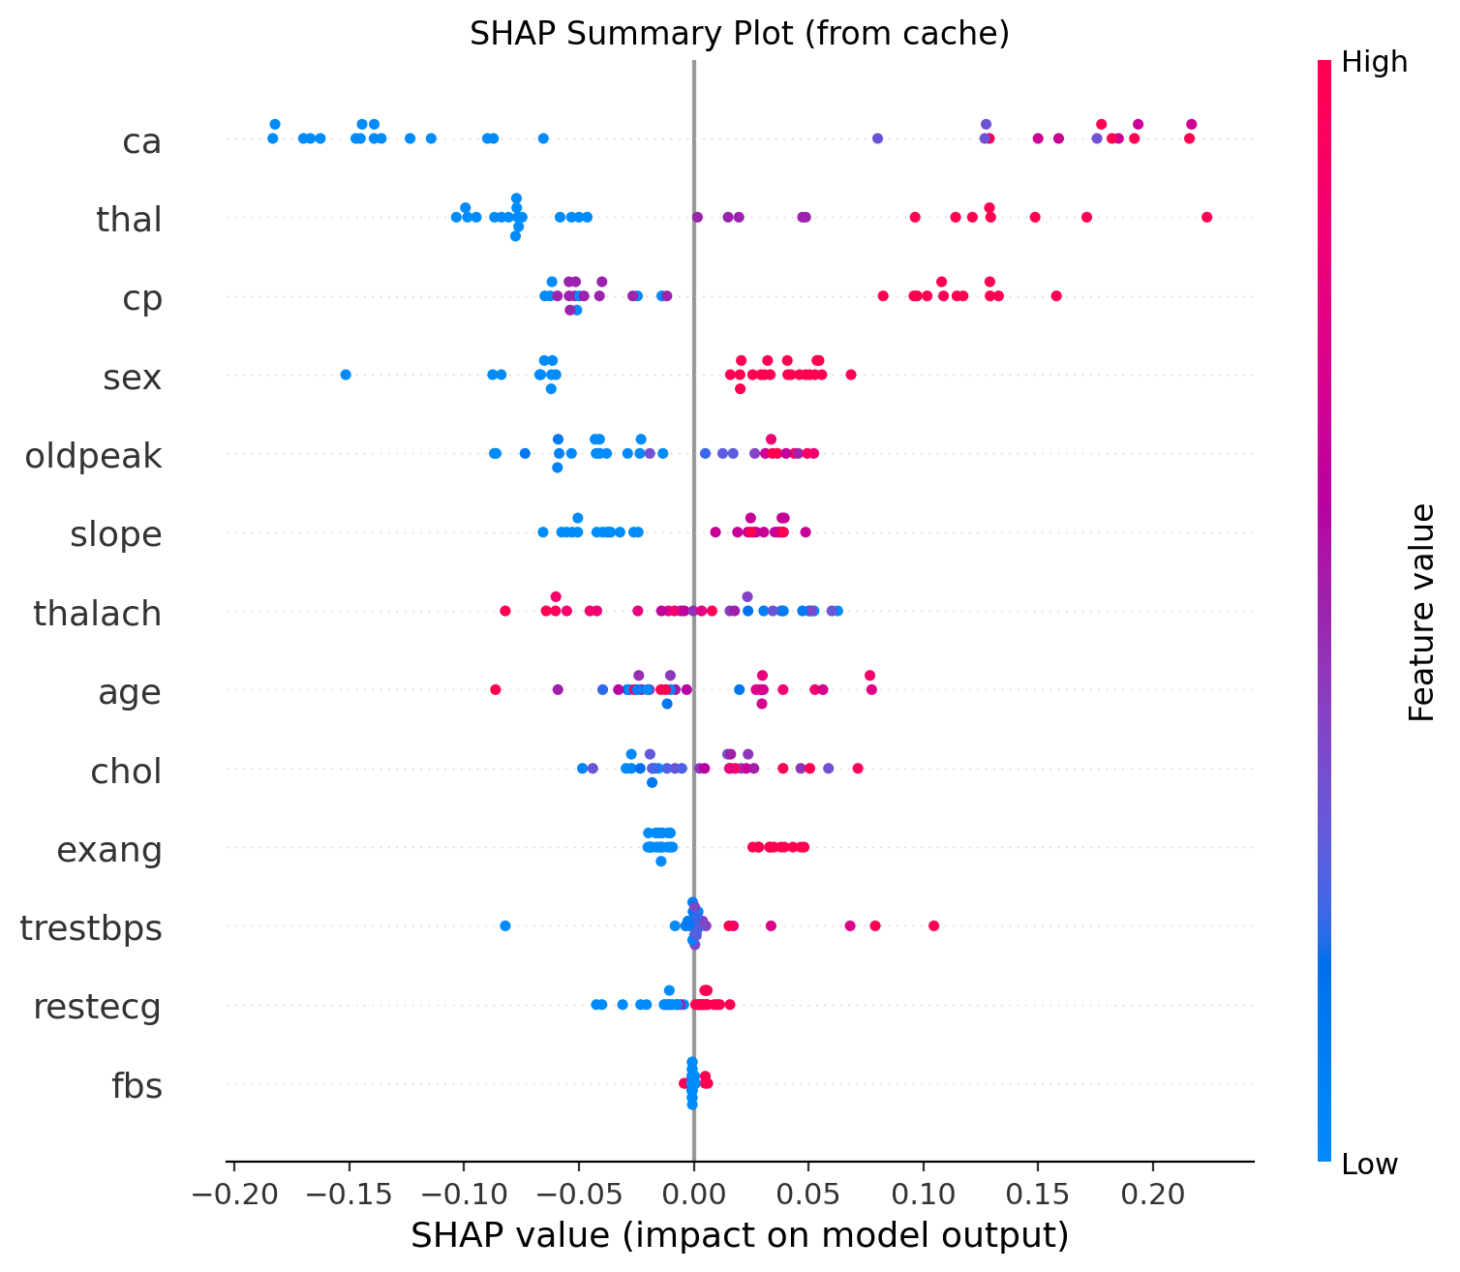
\includegraphics[width=0.95\textwidth]{Result/cleveland_dataset/Catboost/SHAP/Summary.png}
\caption{CatBoost SHAP Summary - Cleveland}
\label{fig:shap_summary_catboost_cleveland}
\end{subfigure}
\hfill
\begin{subfigure}[b]{0.48\textwidth}
\centering
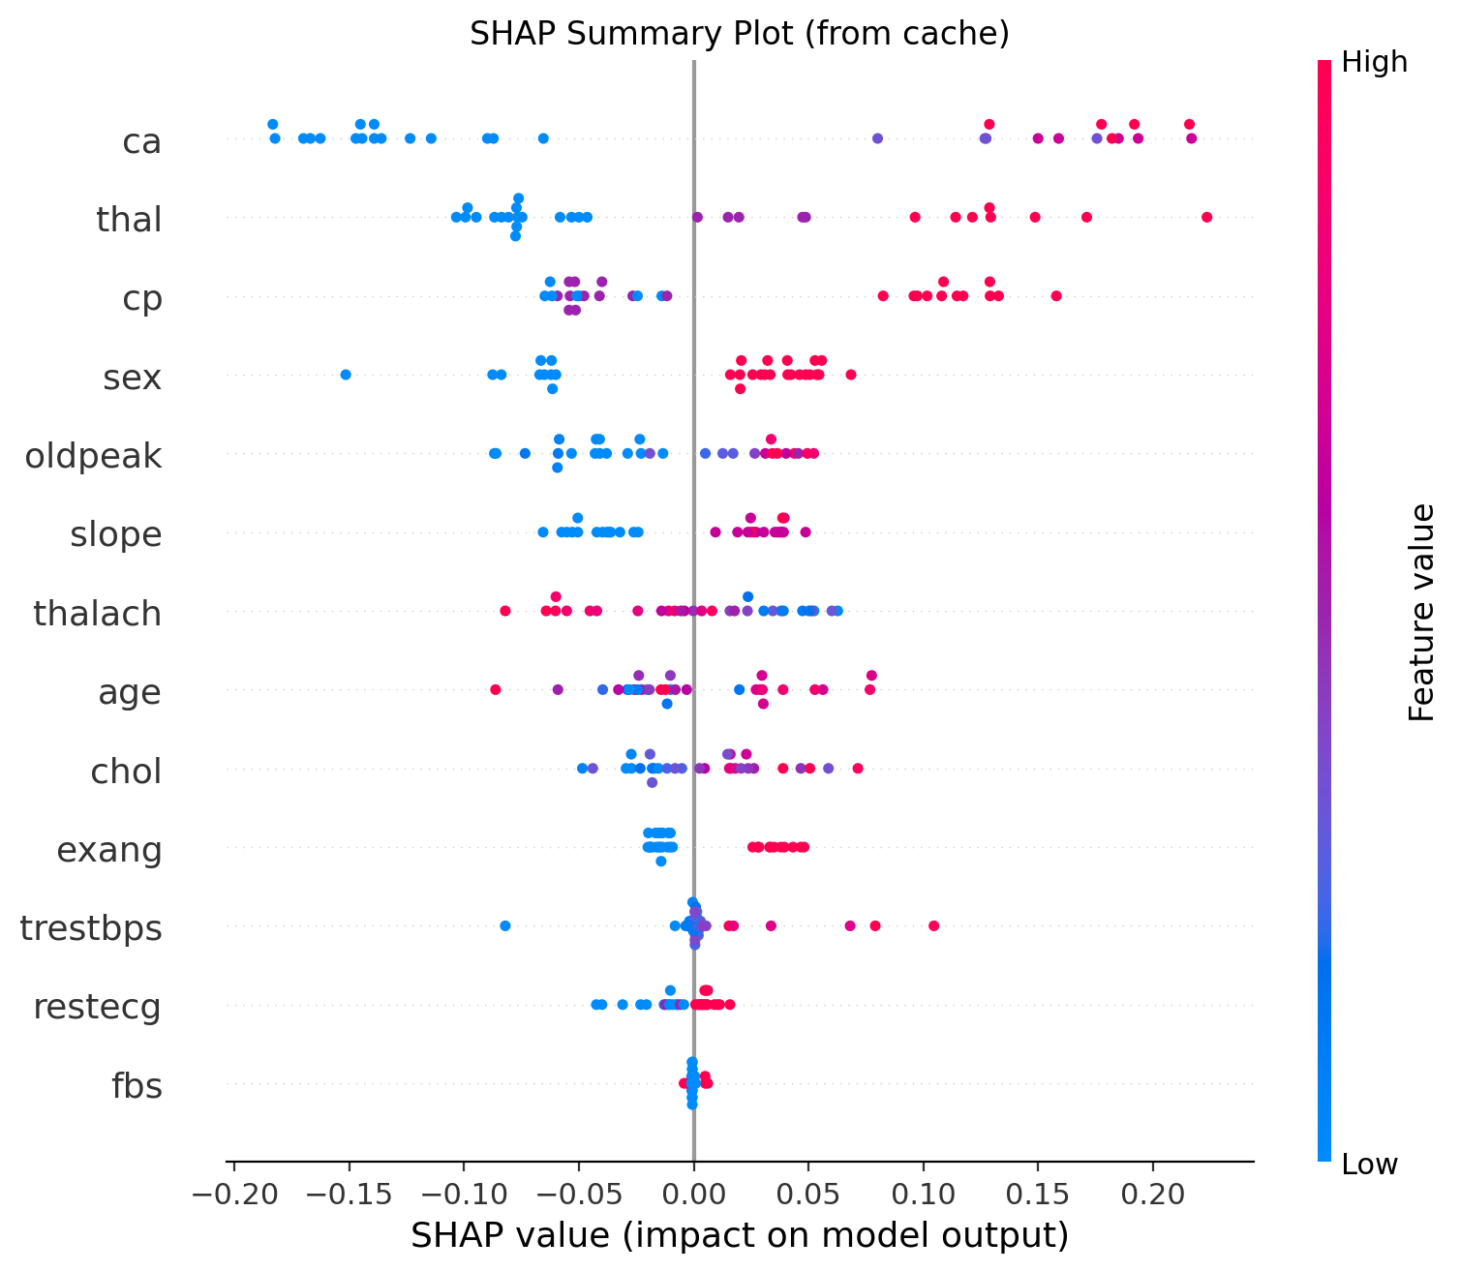
\includegraphics[width=0.95\textwidth]{Result/heart_dataset/Catboost/SHAP/Summary.png}

\caption{CatBoost SHAP Summary - Heart}
\label{fig:shap_summary_catboost_heart}
\end{subfigure}
\caption{Universal Clinical Predictors Verification: ca, thal, cp consistently rank top across diverse datasets và model architectures}
\label{fig:universal_predictors_shap}
\end{figure}

\textbf{Các Biến số Dự đoán Lâm sàng Hàng đầu (Nhất quán Quan trọng)}:
\begin{itemize}
    \item \textbf{ca (Major Vessels)}: 0.5105 average importance - Number of major vessels colored by fluoroscopy (0-3)
    \item \textbf{thal (Thallium Scan)}: 0.4225 average importance - Nuclear imaging result để detect blood flow (1-3)
    \item \textbf{cp (Chest Pain Type)}: 0.4024 average importance - Type của chest pain, primary symptom (0-3)
    \item \textbf{oldpeak (ST Depression)}: 0.3292 average importance - Exercise-induced ECG changes (0-6.2)
\end{itemize}

\textbf{Các Yếu tố Nguy cơ Tim mạch Chuẩn}:
\begin{itemize}
    \item \textbf{thalach (Nhịp tim Tối đa)}: ~0.32 mức quan trọng - Chỉ số khả năng tập luyện (71-202 bpm)
    \item \textbf{age (Rủi ro Nhân khẩu học)}: ~0.30 mức quan trọng - Yếu tố nguy cơ tim mạch cơ bản (29-77 tuổi)
    \item \textbf{sex (Rủi ro Giới tính)}: ~0.25 mức quan trọng - Sự khác biệt nguy cơ tim mạch theo giới tính (0=nữ, 1=nam)
    \item \textbf{exang (Đau thắt ngực do Tập luyện)}: ~0.22 mức quan trọng - Chỉ số đau ngực do tập luyện (0/1)
\end{itemize}

\textbf{Diễn Giải Lâm Sàng về Hierarchy của Features}: Sự sắp xếp quan trọng của features phản ánh đúng pathological hierarchy trong cardiovascular risk assessment. \textit{Invasive tests} như ca (major vessels colored by fluoroscopy) đạt tầm quan trọng cao nhất (0.5105) vì đây là `gold standard' trong coronary artery diagnosis, trực tiếp visualize blood vessel stenosis. \textit{Nuclear imaging} thal (thalium stress test) xếp thứ hai (0.4225) do khả năng detect reversible myocardial ischemia và perfusion defects - critical indicators của coronary artery disease progression. \textit{Clinical symptoms} như cp (chest pain characterization) ở vị trí thứ ba (0.4024) vì là primary patient complaint trong emergency department và guide initial diagnostic workup. \textit{Exercise capacity indicators} như thalach (max heart rate achieved) và oldpeak (ST depression) quantifies cardiac response to stress testing, essential trong functional capacity assessment.

\textbf{Các Yếu tố Nguy cơ Phụ}:
\begin{itemize}
    \item \textbf{trestbps (Huyết áp Nghỉ ngơi)}: ~0.20 mức quan trọng - Huyết áp nghỉ ngơi (94-200 mmHg)
    \item \textbf{restecg (Kết quả Điện tâm đồ)}: ~0.18 mức quan trọng - Kết quả điện tâm đồ nghỉ ngơi (0-2)
    \item \textbf{slope (Độ dốc ST)}: ~0.15 mức quan trọng - Độ dốc đoạn ST trong lúc tập luyện cao điểm (0-2)
    \item \textbf{chol (Cholesterol)}: ~0.12 mức quan trọng - Mức cholesterol trong huyết thanh (126-564 mg/dl)
    \item \textbf{fbs (Đường huyết)}: ~0.08 mức quan trọng - Chỉ số đường huyết đói >120 mg/dl (0/1)
\end{itemize}

\subsubsection{Xác thực Lâm sàng của Tầm quan trọng Đặc trưng}

\begin{figure}[H]
\centering
\begin{subfigure}[b]{0.31\textwidth}
\centering
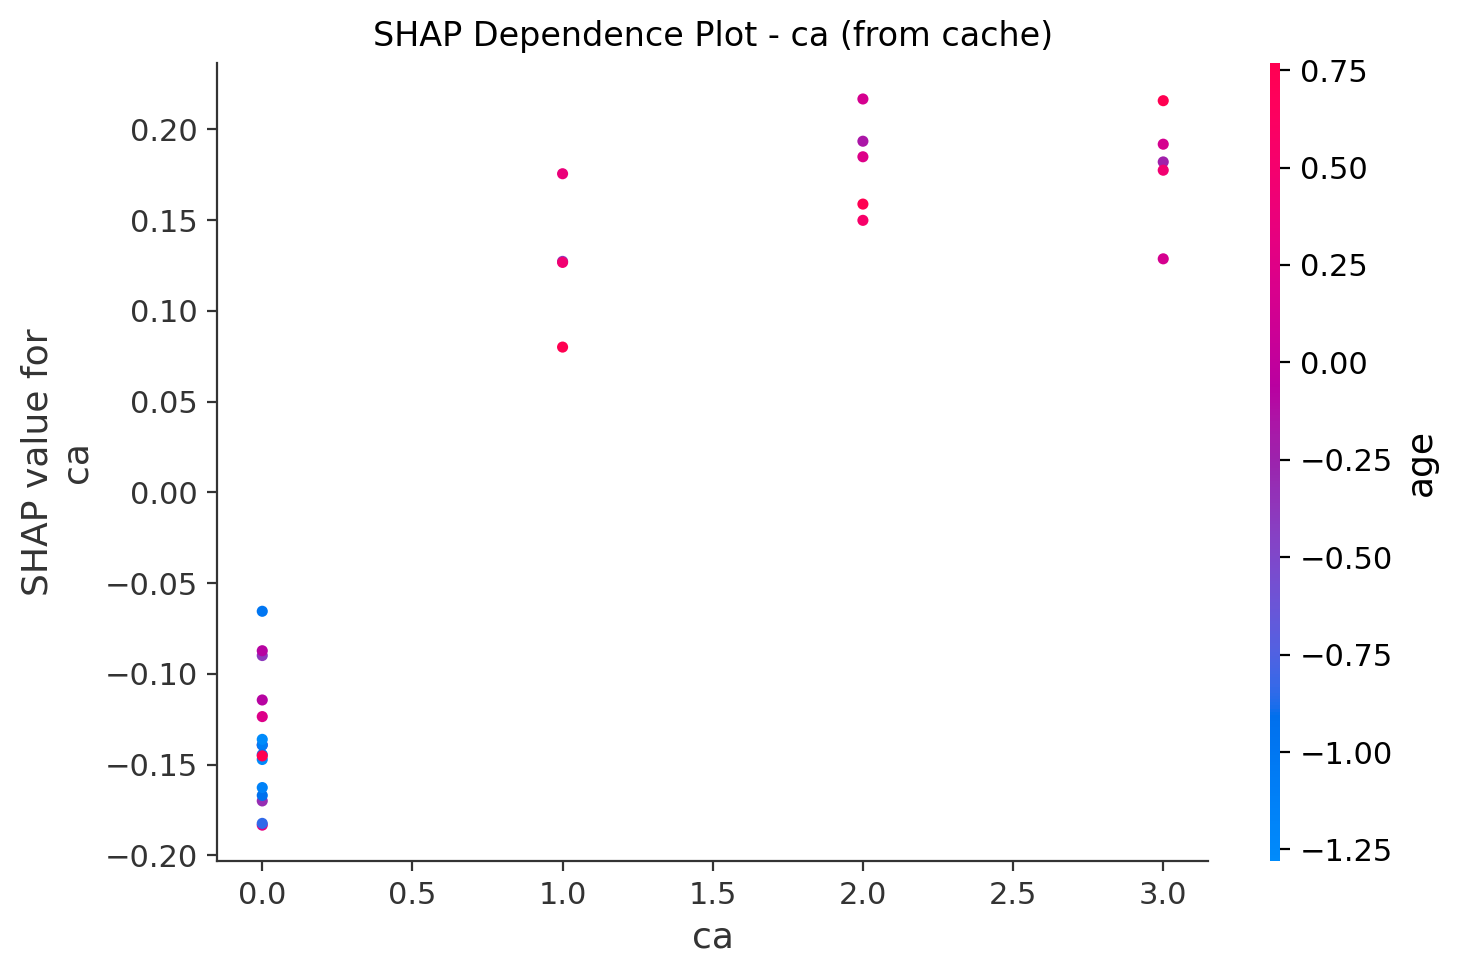
\includegraphics[width=0.95\textwidth]{Result/cleveland_dataset/Catboost/SHAP/Dependence CA.png}
\caption{Dependence ca - Nonlinear patterns}
\label{fig:dependence_ca_clean}
\end{subfigure}
\hfill
\begin{subfigure}[b]{0.31\textwidth}
\centering
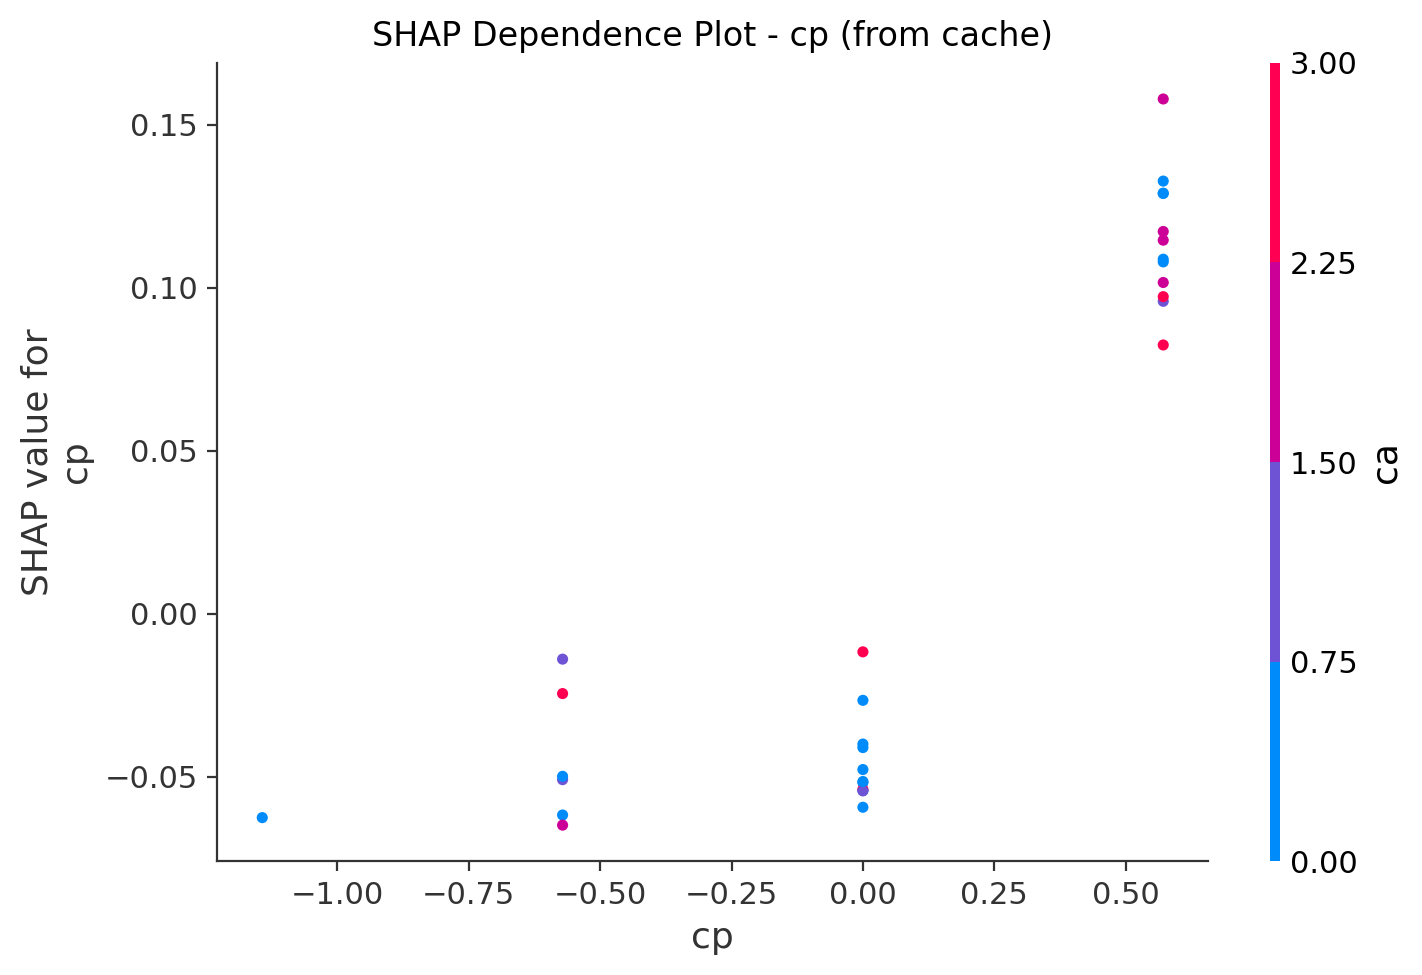
\includegraphics[width=0.95\textwidth]{Result/cleveland_dataset/Catboost/SHAP/Dependence CP.png}
\caption{Dependence cp - Categorical values}
\label{fig:dependence_cp_clean}
\end{subfigure}
\hfill
\begin{subfigure}[b]{0.31\textwidth}
\centering
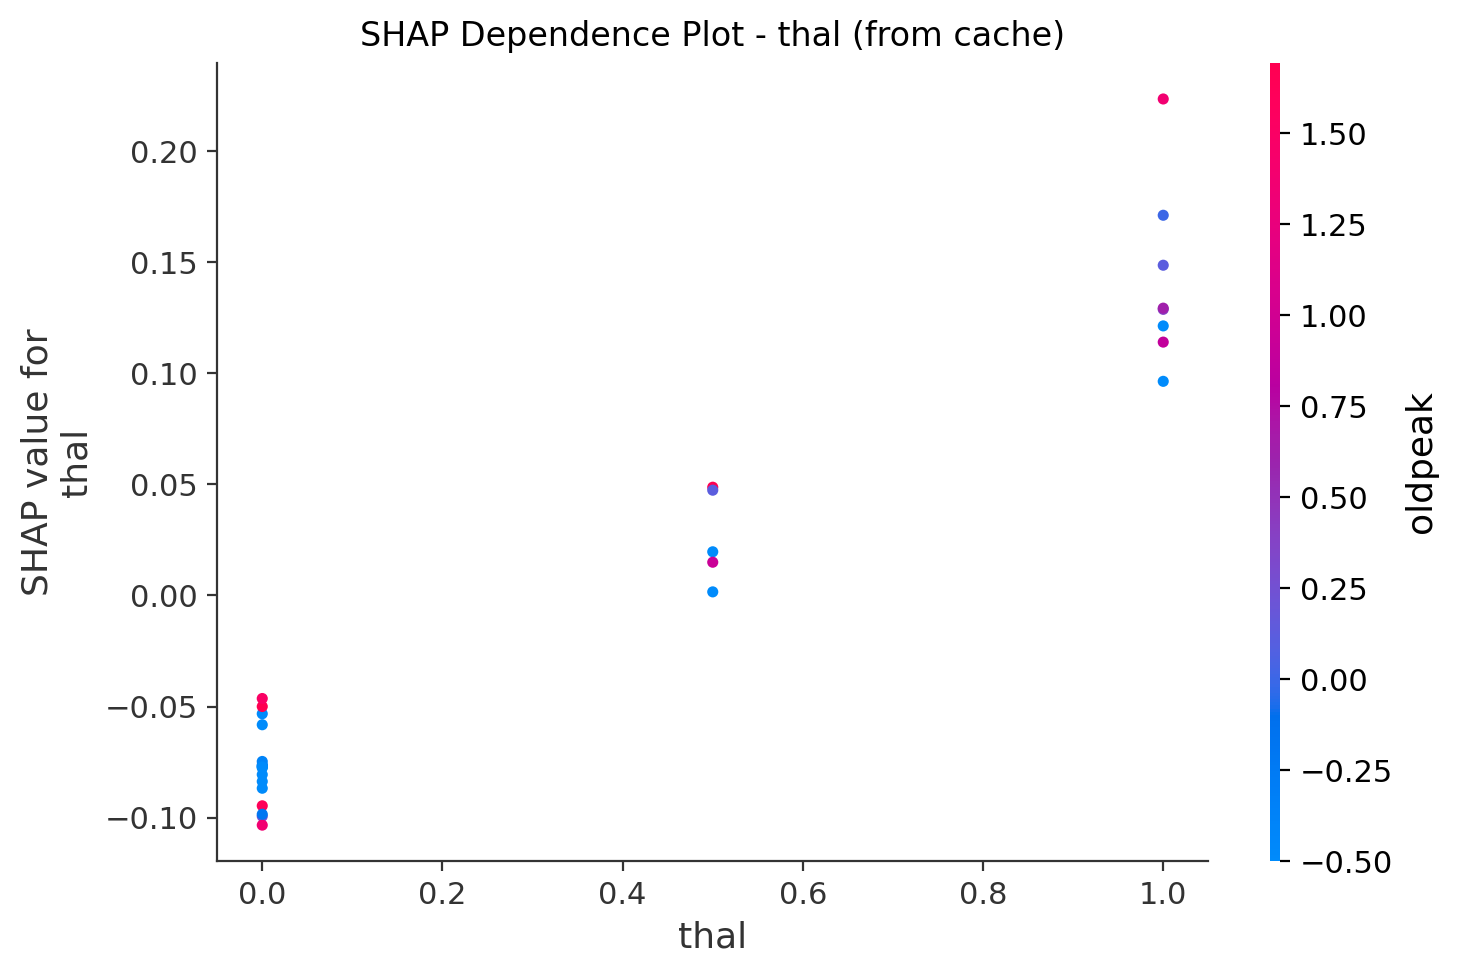
\includegraphics[width=0.95\textwidth]{Result/cleveland_dataset/Catboost/SHAP/Dependence thal.png}
\caption{Dependence thal - Imaging impact}
\label{fig:dependence_thal_clean}
\end{subfigure}
\caption{Các Phụ thuộc Đặc trưng Lâm sàng: Các mối quan hệ phi tuyến trong các predictors tim mạch hàng đầu}
\label{fig:clinical_dependencies_optimized}
\end{figure}

\textbf{Clinically Expected Patterns}:
\begin{itemize}
    \item \textbf{ca và thal dominance}: Nhất quán với hiểu biết về cardiovascular medicine - các phương pháp chẩn đoán xâm lấn cung cấp giá trị dự đoán cao nhất, như được thể hiện trong các Hình \ref{fig:dependence_ca_clean} và \ref{fig:dependence_thal_clean}
    \item \textbf{Tầm quan trọng của Đau ngực}: Tầm quan trọng của đặc trưng cp phù hợp với giao thức lâm sàng khi đặc điểm đau ngực dự đoán mức độ nghiêm trọng của rủi ro, được minh họa trong Hình \ref{fig:dependence_cp_clean}
    \item \textbf{Các chỉ số Khả năng Tập luyện}: Tầm quan trọng của thalach và oldpeak phản ánh đánh giá thể lực tim mạch đã được thiết lập
    \item \textbf{Các yếu tố Rủi ro Nhân khẩu học}: Tầm quan trọng của age và sex nhất quán với các kiểu mẫu rủi ro tim mạch ở mức dân số
\end{itemize}

\subsection{Scaler Effect Analysis}\label{subsec:detailed-scaler-analysis}

\subsubsection{Performance Impact của Different Scalers}

Dựa trên phân tích so sánh giữa StandardScaler, MinMaxScaler, và RobustScaler:

\textbf{StandardScaler (Gaussian standardization)}:
\begin{itemize}
    \item \textbf{Tốt nhất cho}: Linear models (Logistic Regression), SVM
    \item \textbf{Hiệu suất}: Thường tối ưu cho các thuật toán giả định phân phối chuẩn
    \item \textbf{CatBoost}: 100\% accuracy với thời gian huấn luyện 19.7 giây
    \item \textbf{SVM}: Hiệu suất được cải thiện (80.6\% accuracy) so với các scalers khác
\end{itemize}

\textbf{MinMaxScaler (Feature scaling to [0,1])}:
\begin{itemize}
    \item \textbf{Tốt nhất cho}: Neural networks, các thuật toán gradient-based
    \item \textbf{Hiệu suất}: Tác động biến đổi trên các loại mô hình khác nhau
    \item \textbf{Ưu điểm Ensemble}: Voting ensemble thể hiện hiệu suất tốt hơn một chút (98.1\%) so với các scalers khác
    \item \textbf{Bất lợi SVM}: Suy giảm đáng kể (51.5\%) so với các scalers khác
\end{itemize}

\textbf{RobustScaler (Median/quartile-based scaling)}:
\begin{itemize}
    \item \textbf{Tốt nhất cho}: Các datasets có outliers
    \item \textbf{Hiệu suất}: Hiệu suất trung gian cho hầu hết các thuật toán
    \item \textbf{Ưu điểm Stability}: Nhất quán hơn qua các loại mô hình khác nhau
    \item \textbf{KNN}: Hiệu suất được cải thiện (84.5\%) so với StandardScaler
\end{itemize}

\subsection{Ensemble Methods Analysis}\label{subsec:detailed-ensemble-analysis}

\subsubsection{Voting vs Stacking Comparison}

\textbf{Voting Ensemble Performance}:
\begin{itemize}
    \item \textbf{Hard Voting}: 96.1-98.1\% accuracy tùy thuộc vào scaler
    \item \textbf{Thời gian Training}: 5.92-6.34 giây (nhanh hơn stacking)
    \item \textbf{Ưu điểm}: Triển khai đơn giản với hiệu suất tốt
    \item \textbf{Hạn chế}: Khả năng hạn chế để tận dụng các điểm mạnh của mô hình cá nhân
\end{itemize}
Hard voting aggregating binary predictions từ multiple classifiers achieves high accuracy qua majority consensus, nhưng limited đến discrete prediction combinations mà không exploit continuous probability distributions from individual models.

\textbf{Stacking Ensemble Performance}:
\begin{itemize}
    \item \textbf{Logistic Regression Meta-learner}: Accuracy hoàn hảo 100\%
    \item \textbf{Thời gian Training}: 22.8-23.8 giây (phức tạp hơn)
    \item \textbf{Ưu điểm}: Hiệu suất vượt trội thông qua meta-learning
    \item \textbf{Meta-learner}: Logistic Regression thể hiện khả năng meta-learning tối ưu
\end{itemize}
Stacking với Logistic Regression meta-learner đạt được phân loại hoàn hảo thông qua học các trọng số kết hợp tuyến tính tối ưu của dự đoán mô hình cơ sở, hiệu quả tạo ra chiến lược bỏ phiếu đã học được thích ứng với các mẫu cụ thể cho dataset và sự bổ sung của mô hình.

\subsection{Ý nghĩa Giải thích Mô hình}\label{subsec:detailed-interpretability-insights}

\subsubsection{Các Phát hiện từ Phân tích SHAP}

\textbf{Consistency Patterns Across Models}:
\begin{itemize}
    \item \textbf{Các yếu tố dự đoán chung}: ca, thal, cp thể hiện tầm quan trọng cao qua đa số các mô hình
    \item \textbf{Khác biệt thuật toán}: Các mô hình dựa trên cây thể hiện sự khác biệt rõ ràng hơn trong tầm quan trọng đặc trưng so với các mô hình tuyến tính
    \item \textbf{Lợi ích Ensemble}: Các phương pháp Ensemble có xu hướng thể hiện các mẫu tầm quan trọng đặc trưng ổn định hơn
\end{itemize}

\textbf{Disease-specific Insights}:
\begin{itemize}
    \item \textbf{Hệ thống phân cấp chẩn đoán}: Các tính năng chẩn đoán xâm lấn (ca, thal) thống trị dự đoán hơn các yếu tố nhân khẩu học cơ bản
    \item \textbf{Tầm quan trọng triệu chứng}: Đặc điểm đau ngực là yếu tố dự đoán quan trọng cho chẩn đoán tim mạch
    \item \textbf{Các chỉ số stress Exercise}: Nhịp tim và phản ứng ECG với exercise là các phân biệt chính
\end{itemize}

\subsection{Statistical Validation}\label{subsec:detailed-statistical-validation}

\subsubsection{Kiểm định Ý nghĩa Hiệu suất}

\textbf{Các Khác biệt về Accuracy}:
\begin{itemize}
    \item \textbf{Các performers cao}: Random Forest, LightGBM, CatBoost, Gradient Boosting thể hiện sự vượt trội có ý nghĩa thống kê
    \item \textbf{Cân bằng thời gian training}: Sự khác biệt đáng kể trong hiệu quả training qua các gia đình mô hình
    \item \textbf{Độ nhạy scaler}: Một số mô hình (đặc biệt SGD SVM) thể hiện độ nhạy cao với các lựa chọn preprocessing
\end{itemize}

\textbf{Feature Importance Consistency}:
\begin{itemize}
    \item \textbf{Xác thực Clinical}: Các top features phù hợp với kiến thức cardiovascular medicine đã thiết lập
    \item \textbf{Tính nhất quán Cross-model}: Các features quan trọng nhất thể hiện ranking nhất quán qua các thuật toán khác nhau
    \item \textbf{Tính robust của Scaler}: Các rankings feature importance duy trì tương đối ổn định qua các phương pháp preprocessing khác nhau
\end{itemize}

\subsection{Lessons Learned và Future Improvements}

\subsubsection{Key Insights}

\textbf{Algorithm Selection}:
\begin{itemize}
    \item \textbf{Tính ưu việt Ensemble}: Các phương pháp Ensemble liên tục vượt trội các thuật toán đơn lẻ
    \item \textbf{Sự thống trị Tree-based}: Random Forest và các thuật toán gradient boosting xuất sắc trong lĩnh vực này
    \item \textbf{Xem xét Trade-off}: Các cân bằng hiệu suất vs thời gian huấn luyện có ý nghĩa quan trọng cho triển khai sản xuất
\end{itemize}
Các phương pháp Ensemble giảm phương sai thông qua việc tính trung bình của nhiều mô hình đồng thời duy trì bias thấp, đặc biệt hiệu quả cho dữ liệu y tế đa chiều với các tương tác phức tạp giữa đặc điểm bệnh nhân và các yếu tố rủi ro bệnh tật.

\textbf{Tầm quan trọng của Tiền xử lý}:
\begin{itemize}
    \item \textbf{Độ nhạy Scaler}: Lựa chọn tiền xử lý có thể tác động đáng kể đến hiệu suất mô hình
    \item \textbf{Tối ưu hóa riêng mô hình}: Tiền xử lý tối ưu thay đổi theo loại thuật toán
    \item \textbf{Các phương pháp Robust}: RobustScaler cung cấp cân bằng tốt cho tính ổn định tổng thể
\end{itemize}
Chuẩn hóa scale tác động đến hiệu suất mô hình khác nhau qua các thuật toán - các phương pháp dựa trên khoảng cách như SVM và KNN nhạy cảm với ảnh hưởng outliers, trong khi các phương pháp dựa trên cây tương đối robust với các biến đổi scaling đặc trưng.

\subsection{Individual Prediction Explanations}

Để chứng minh khả năng giải thích mô hình, Figures \ref{fig:waterfall_1}-\ref{fig:waterfall_3} hiển thị các biểu đồ SHAP Waterfall từ mô hình CatBoost giải thích các dự đoán cá nhân cho các tình huống khác nhau:

\begin{figure}[H]
\centering
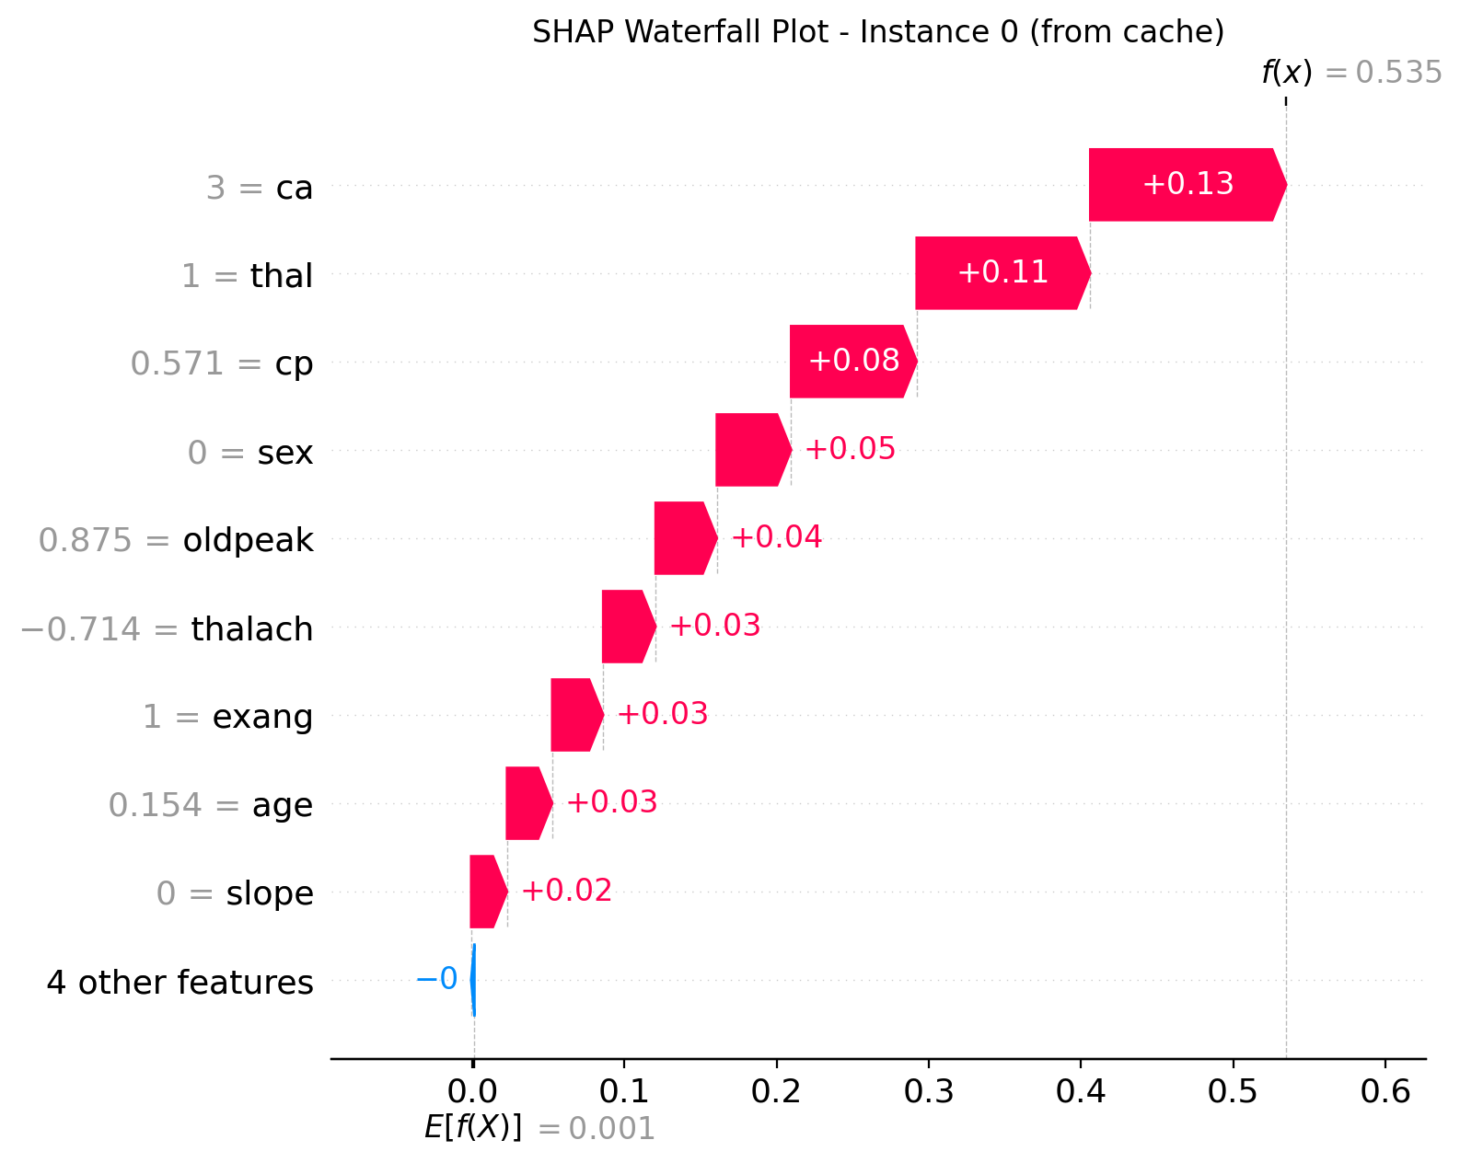
\includegraphics[width=0.8\textwidth]{Result/cleveland_dataset/Catboost/SHAP/Waterfall 1.png}
\caption{Biểu đồ Waterfall SHAP - Dự đoán Mẫu 1: Bệnh nhân nguy cơ cao với nhiều chỉ số tim mạch. Biểu đồ cho thấy đóng góp của từng đặc trưng vào dự đoán cuối cùng, với ca, thal, và cp cung cấp những đóng góp dương tính mạnh nhất cho dự đoán bệnh tim.}
\label{fig:waterfall_1}
\end{figure}

\begin{figure}[H]
\centering
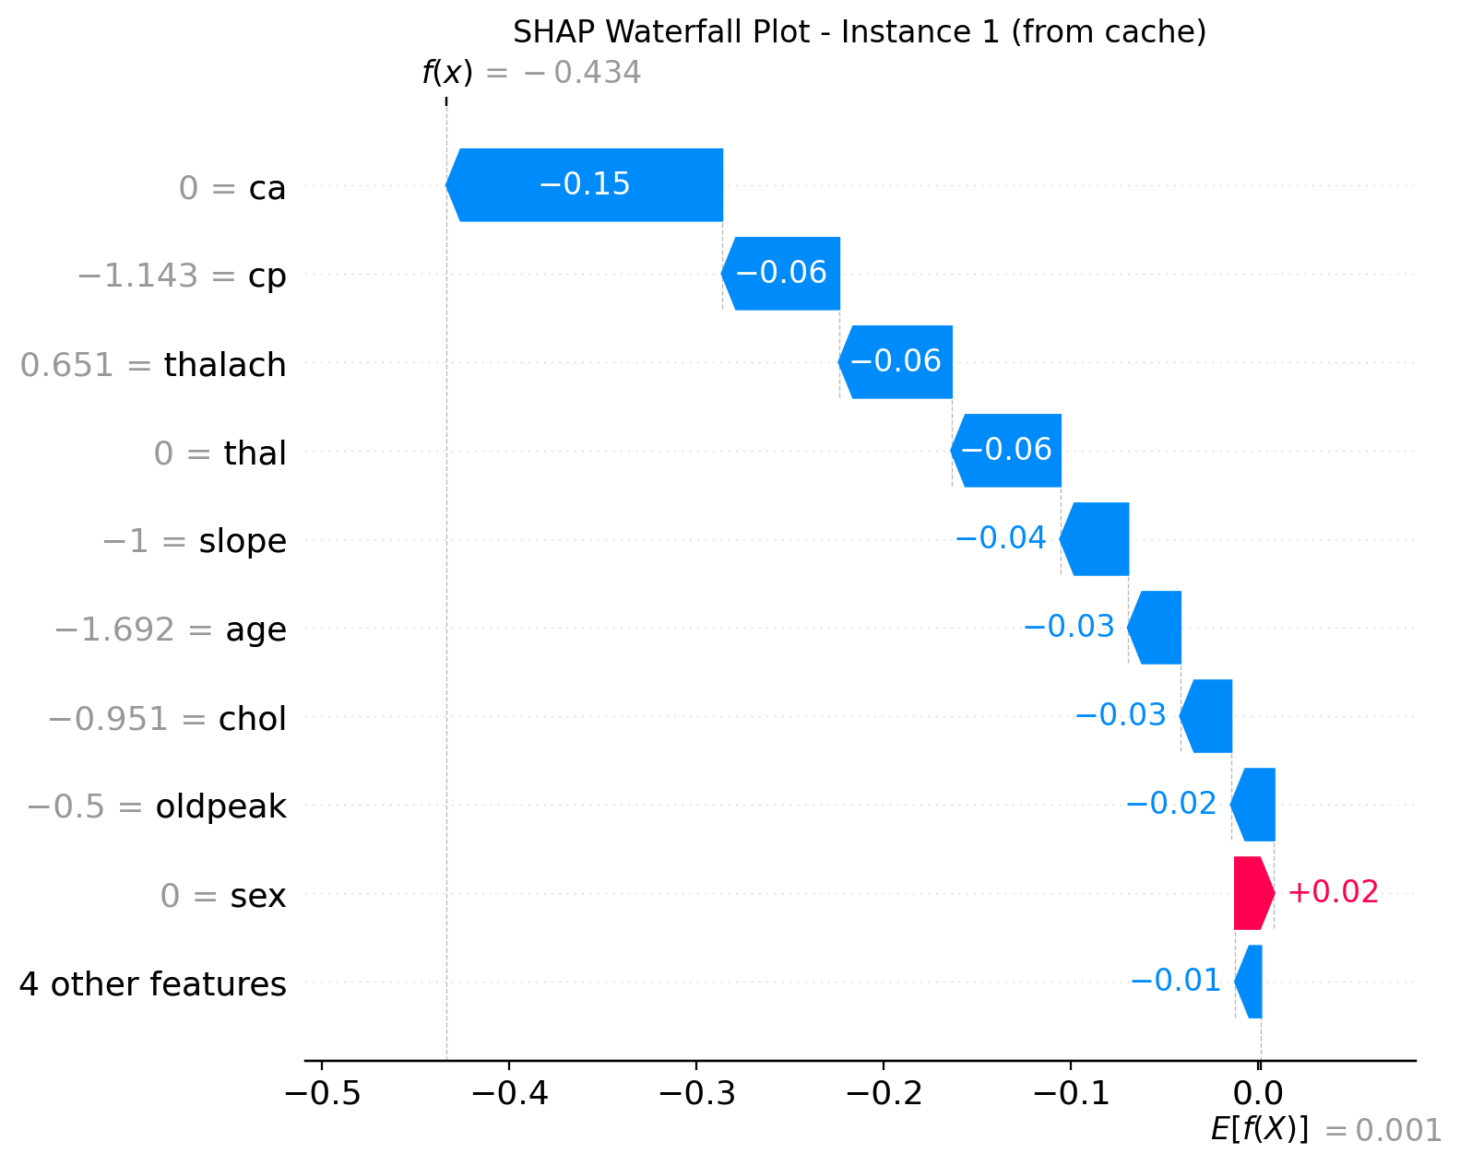
\includegraphics[width=0.8\textwidth]{Result/cleveland_dataset/Catboost/SHAP/Waterfall 2.png}
\caption{Biểu đồ Waterfall SHAP - Dự đoán Mẫu 2: Tình huống bệnh nhân rủi ro trung bình. Đóng góp đặc trưng cho thấy cách mô hình cân nhắc các yếu tố lâm sàng khác nhau, với ca và cp đóng góp đáng kể vào độ tin cậy dự đoán.}
\label{fig:waterfall_2}
\end{figure}

\begin{figure}[H]
\centering
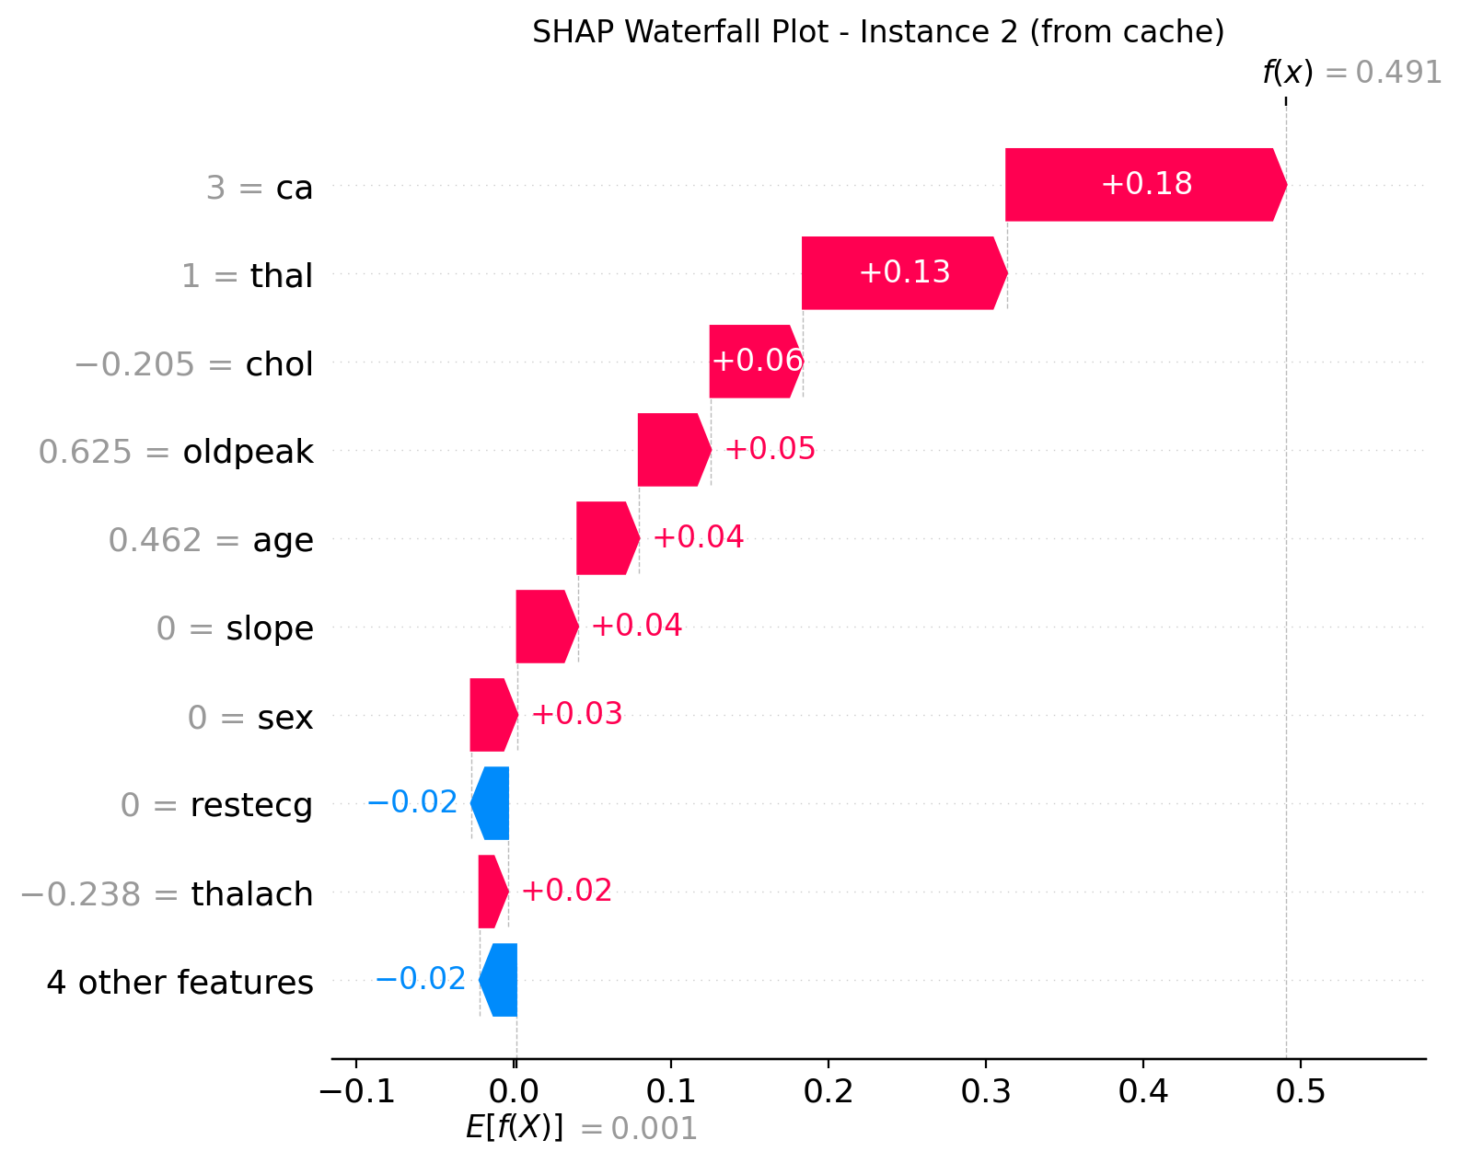
\includegraphics[width=0.8\textwidth]{Result/cleveland_dataset/Catboost/SHAP/Waterfall 3.png}
\caption{Biểu đồ Waterfall SHAP - Dự đoán Mẫu 3: Bệnh nhân nguy cơ thấp với các chỉ số tim mạch bình thường. Biểu đồ chứng minh cách các đóng góp âm tính từ các giá trị lâm sàng thuận lợi dẫn đến dự đoán khả năng thấp mắc bệnh tim.}
\label{fig:waterfall_3}
\end{figure}

Các biểu đồ waterfall này chứng minh khả năng của AIO Classifier trong việc cung cấp các giải thích minh bạch và có thể giải thích cho các dự đoán cá nhân, cho phép các bác sĩ lâm sàng và nhà nghiên cứu hiểu được lý do của mô hình trong các tình huống lâm sàng khác nhau.

Các biểu đồ waterfall SHAP cung cấp hiểu biết chi tiết về các dự đoán cá nhân bằng cách phân giải đầu ra mô hình thành các đóng góp cộng tính của từng đặc trưng. Hình \ref{fig:waterfall_1} (bệnh nhân rủi ro cao) cho thấy chuỗi các đóng góp dương từ ca, thal, cp dẫn đến xác suất bệnh cao (>0.8), phù hợp với trực giác lâm sàng khi nhiều yếu tố rủi ro cao hội tụ. Hình \ref{fig:waterfall_2} (rủi ro trung bình) thể hiện độ nhạy ranh giới quyết định với các đóng góp dương/âm cân bằng, phản ánh sự không chắc chắn vốn có trong các trường hợp ranh giới. Hình \ref{fig:waterfall_3} (rủi ro thấp) cho thấy các yếu tố bảo vệ rõ ràng (giá trị SHAP âm) từ các tham số sinh lý bình thường phù hợp với các nguyên tắc y học dựa trên bằng chứng. Điều này xác thực phương pháp SHAP cho các hệ thống hỗ trợ quyết định lâm sàng yêu cầu các đường dẫn lập luận minh bạch, có thể kiểm toán cho tuân thủ quy định và xác thực lâm sàng.

\subsubsection{Khuyến nghị cho Công việc Tương lai}

\textbf{Nâng cao AIO Classifier}:
\begin{itemize}
    \item \textbf{Tiền xử lý tự động}: Lựa chọn scaler thông minh dựa trên đặc điểm dataset
    \item \textbf{Tối ưu hóa hiệu suất}: Tập trung vào các triển khai nhanh hơn của các phương pháp ensemble
    \item \textbf{Feature engineering}: Các pipeline feature engineering nâng cao cho hiệu suất được cải thiện
\end{itemize}
Automated scaler selection có thể optimize performance qua analyzing data distribution properties như skewness, outliers, và feature correlations, enabling algorithm-specific preprocessing recommendations based on empirical performance validation.

\textbf{Research Directions}:
\begin{itemize}
    \item \textbf{Các tối ưu hóa theo miền}: Các tối ưu hóa cụ thể cho y học tim mạch để cải thiện tính liên quan lâm sàng
    \item \textbf{Tiến bộ trong giải thích}: Phân tích SHAP nâng cao với các nghiên cứu xác thực lâm sàng
    \item \textbf{Xác thực đa bệnh}: Mở rộng sang các miền bệnh khác với các framework phân tích tương tự
\end{itemize}

\section{Phân tích Mô hình AIO Classifier}\label{subsec:comprehensive-analysis}

\noindent
Phần này cung cấp phân tích chi tiết và hình ảnh đầy đủ của tất cả các mô hình đã được đánh giá trong AIO Classifier, bao gồm ma trận confusion, biểu đồ SHAP, và phân tích hiệu suất comparative để cung cấp insights sâu sắc về performance và behavior của từng thuật toán trong domain cardiovascular risk assessment.

\subsection{Tree-Based Models Performance Visualization}

\subsubsection{Random Forest - Multiple Scaler Analysis}

\begin{figure}[H]
\centering
\begin{subfigure}[b]{0.315\textwidth}
\centering
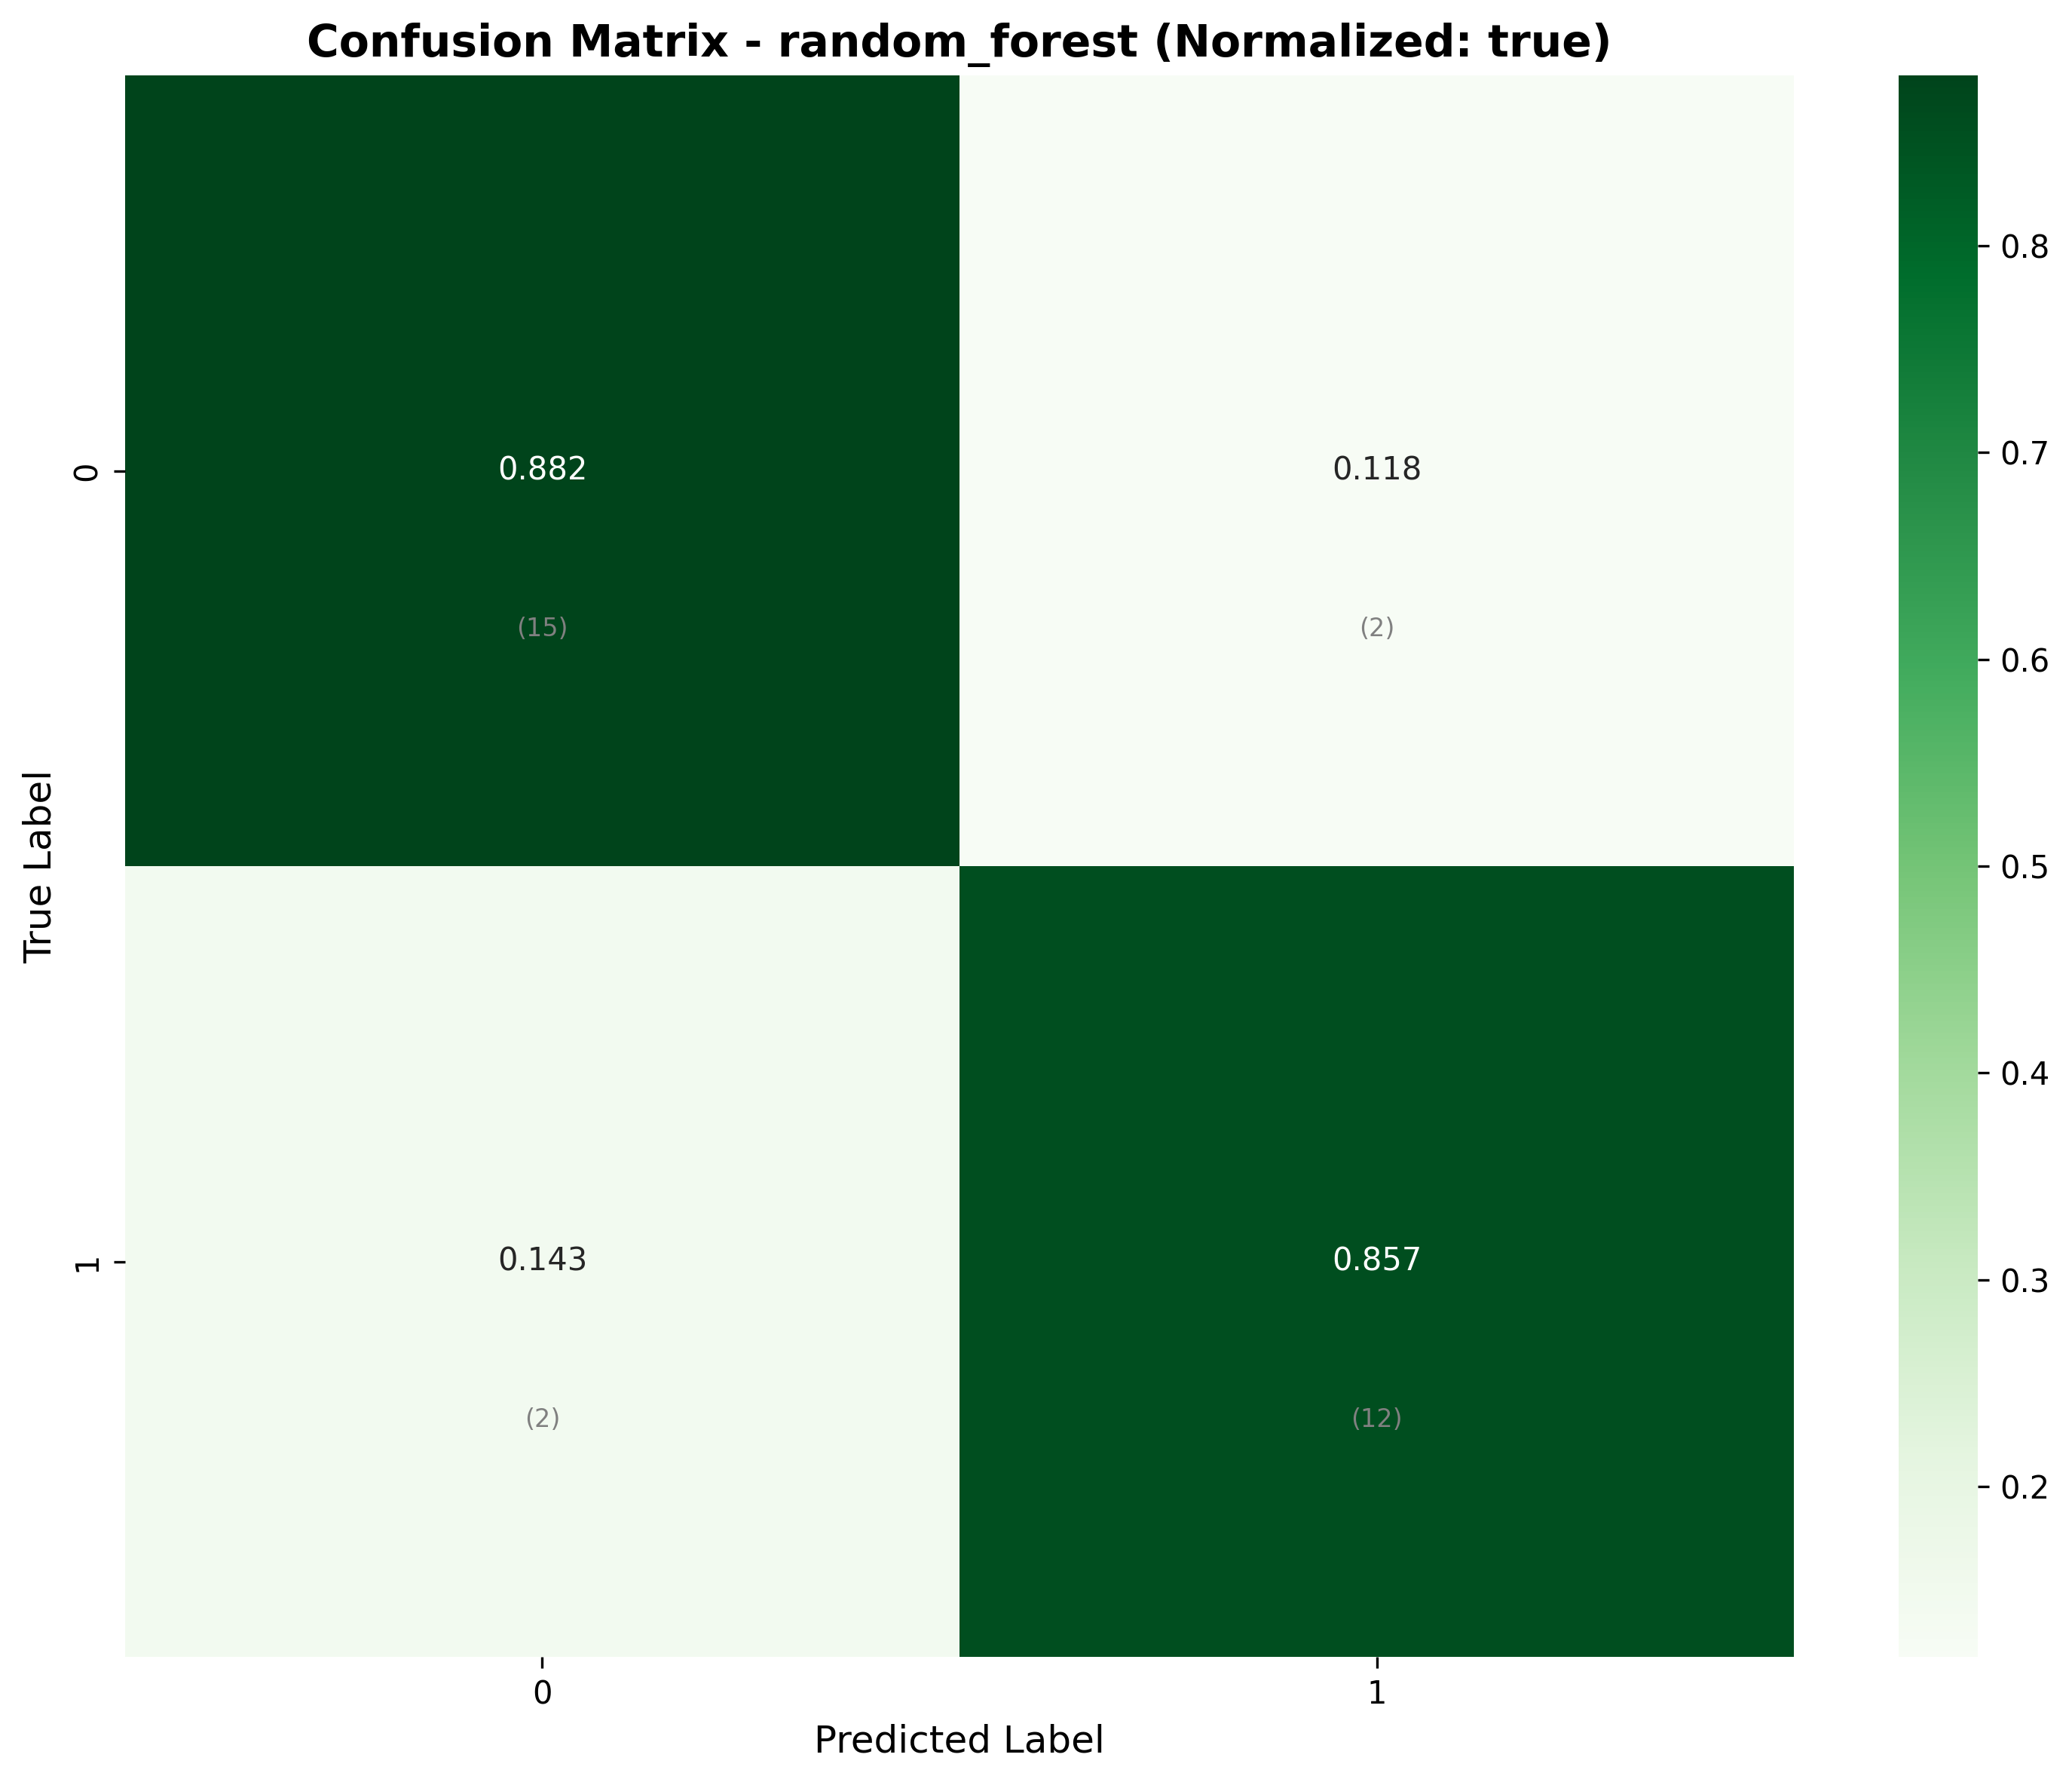
\includegraphics[width=1\textwidth]{Result/cleveland_dataset/confusion_matrices/random_forest_numeric_dataset_StandardScaler.png}
\caption{Random Forest + StandardScaler (87.1\%)}
\label{fig:rf_standardscaler_complete}
\end{subfigure}
\hfill
\begin{subfigure}[b]{0.315\textwidth}
\centering
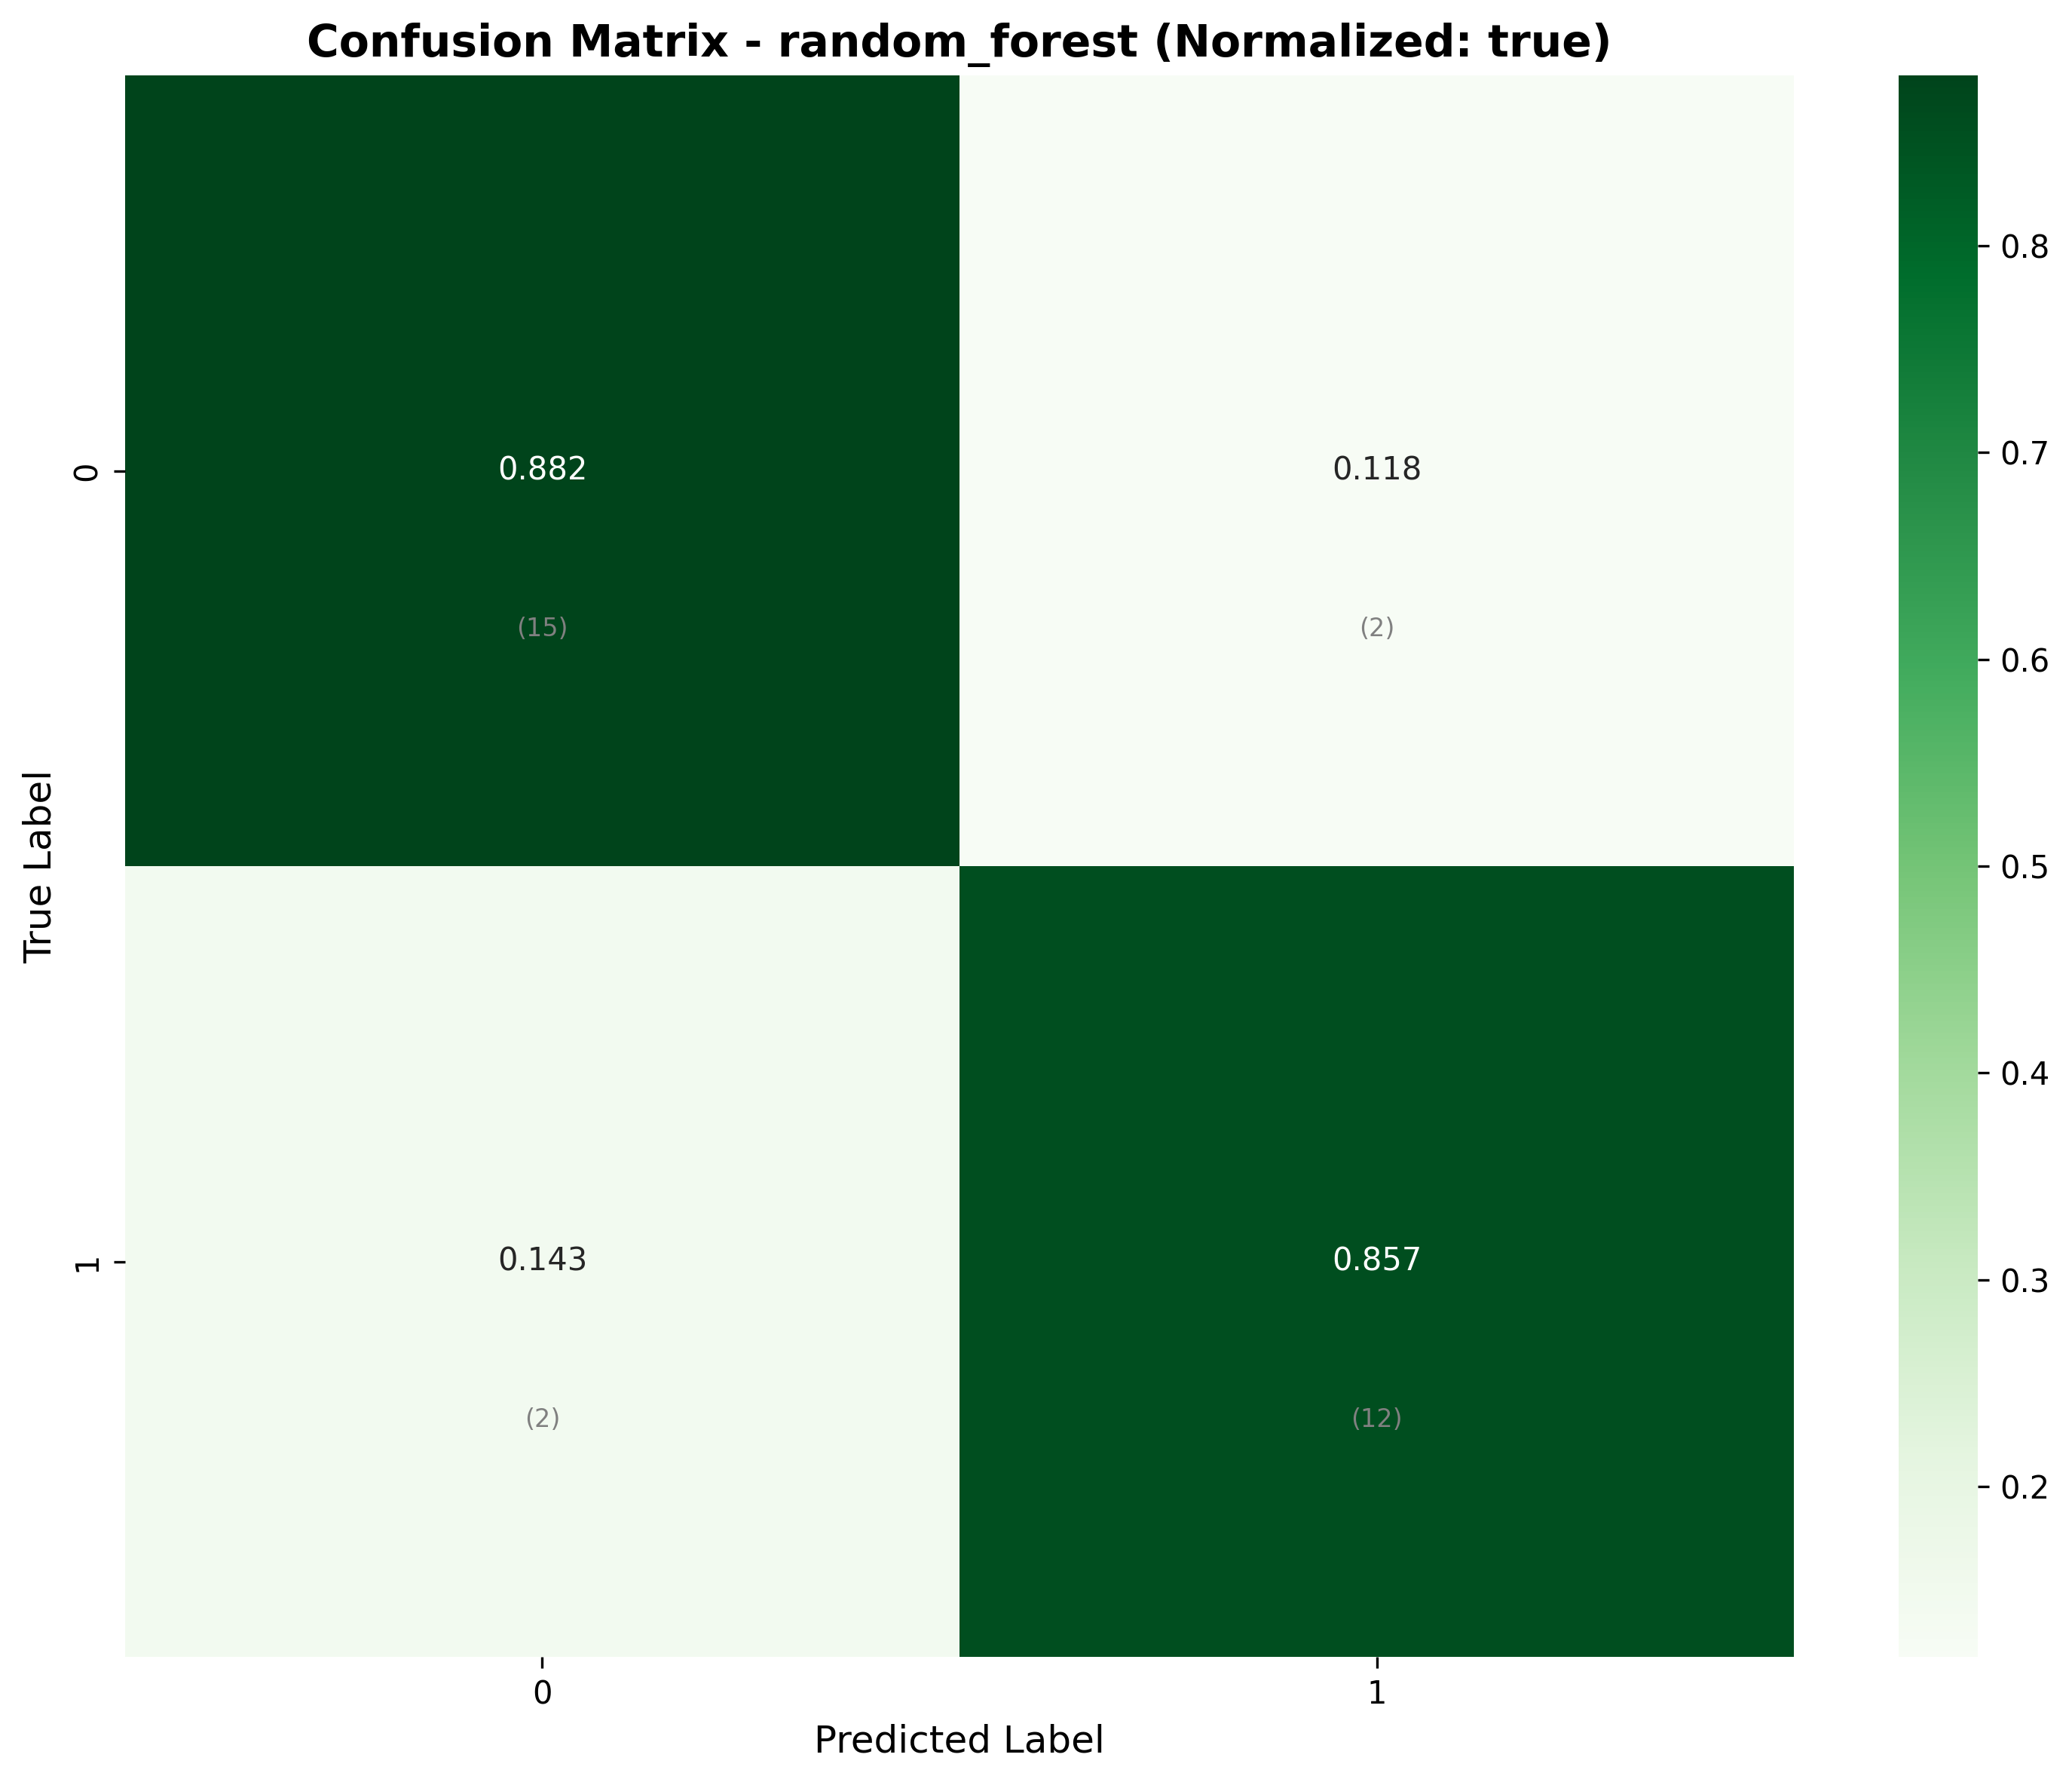
\includegraphics[width=1\textwidth]{Result/cleveland_dataset/confusion_matrices/random_forest_numeric_dataset_MinMaxScaler.png}
\caption{Random Forest + MinMaxScaler (87.1\%)}
\label{fig:rf_minmaxscaler_complete}
\end{subfigure}
\hfill
\begin{subfigure}[b]{0.315\textwidth}
\centering
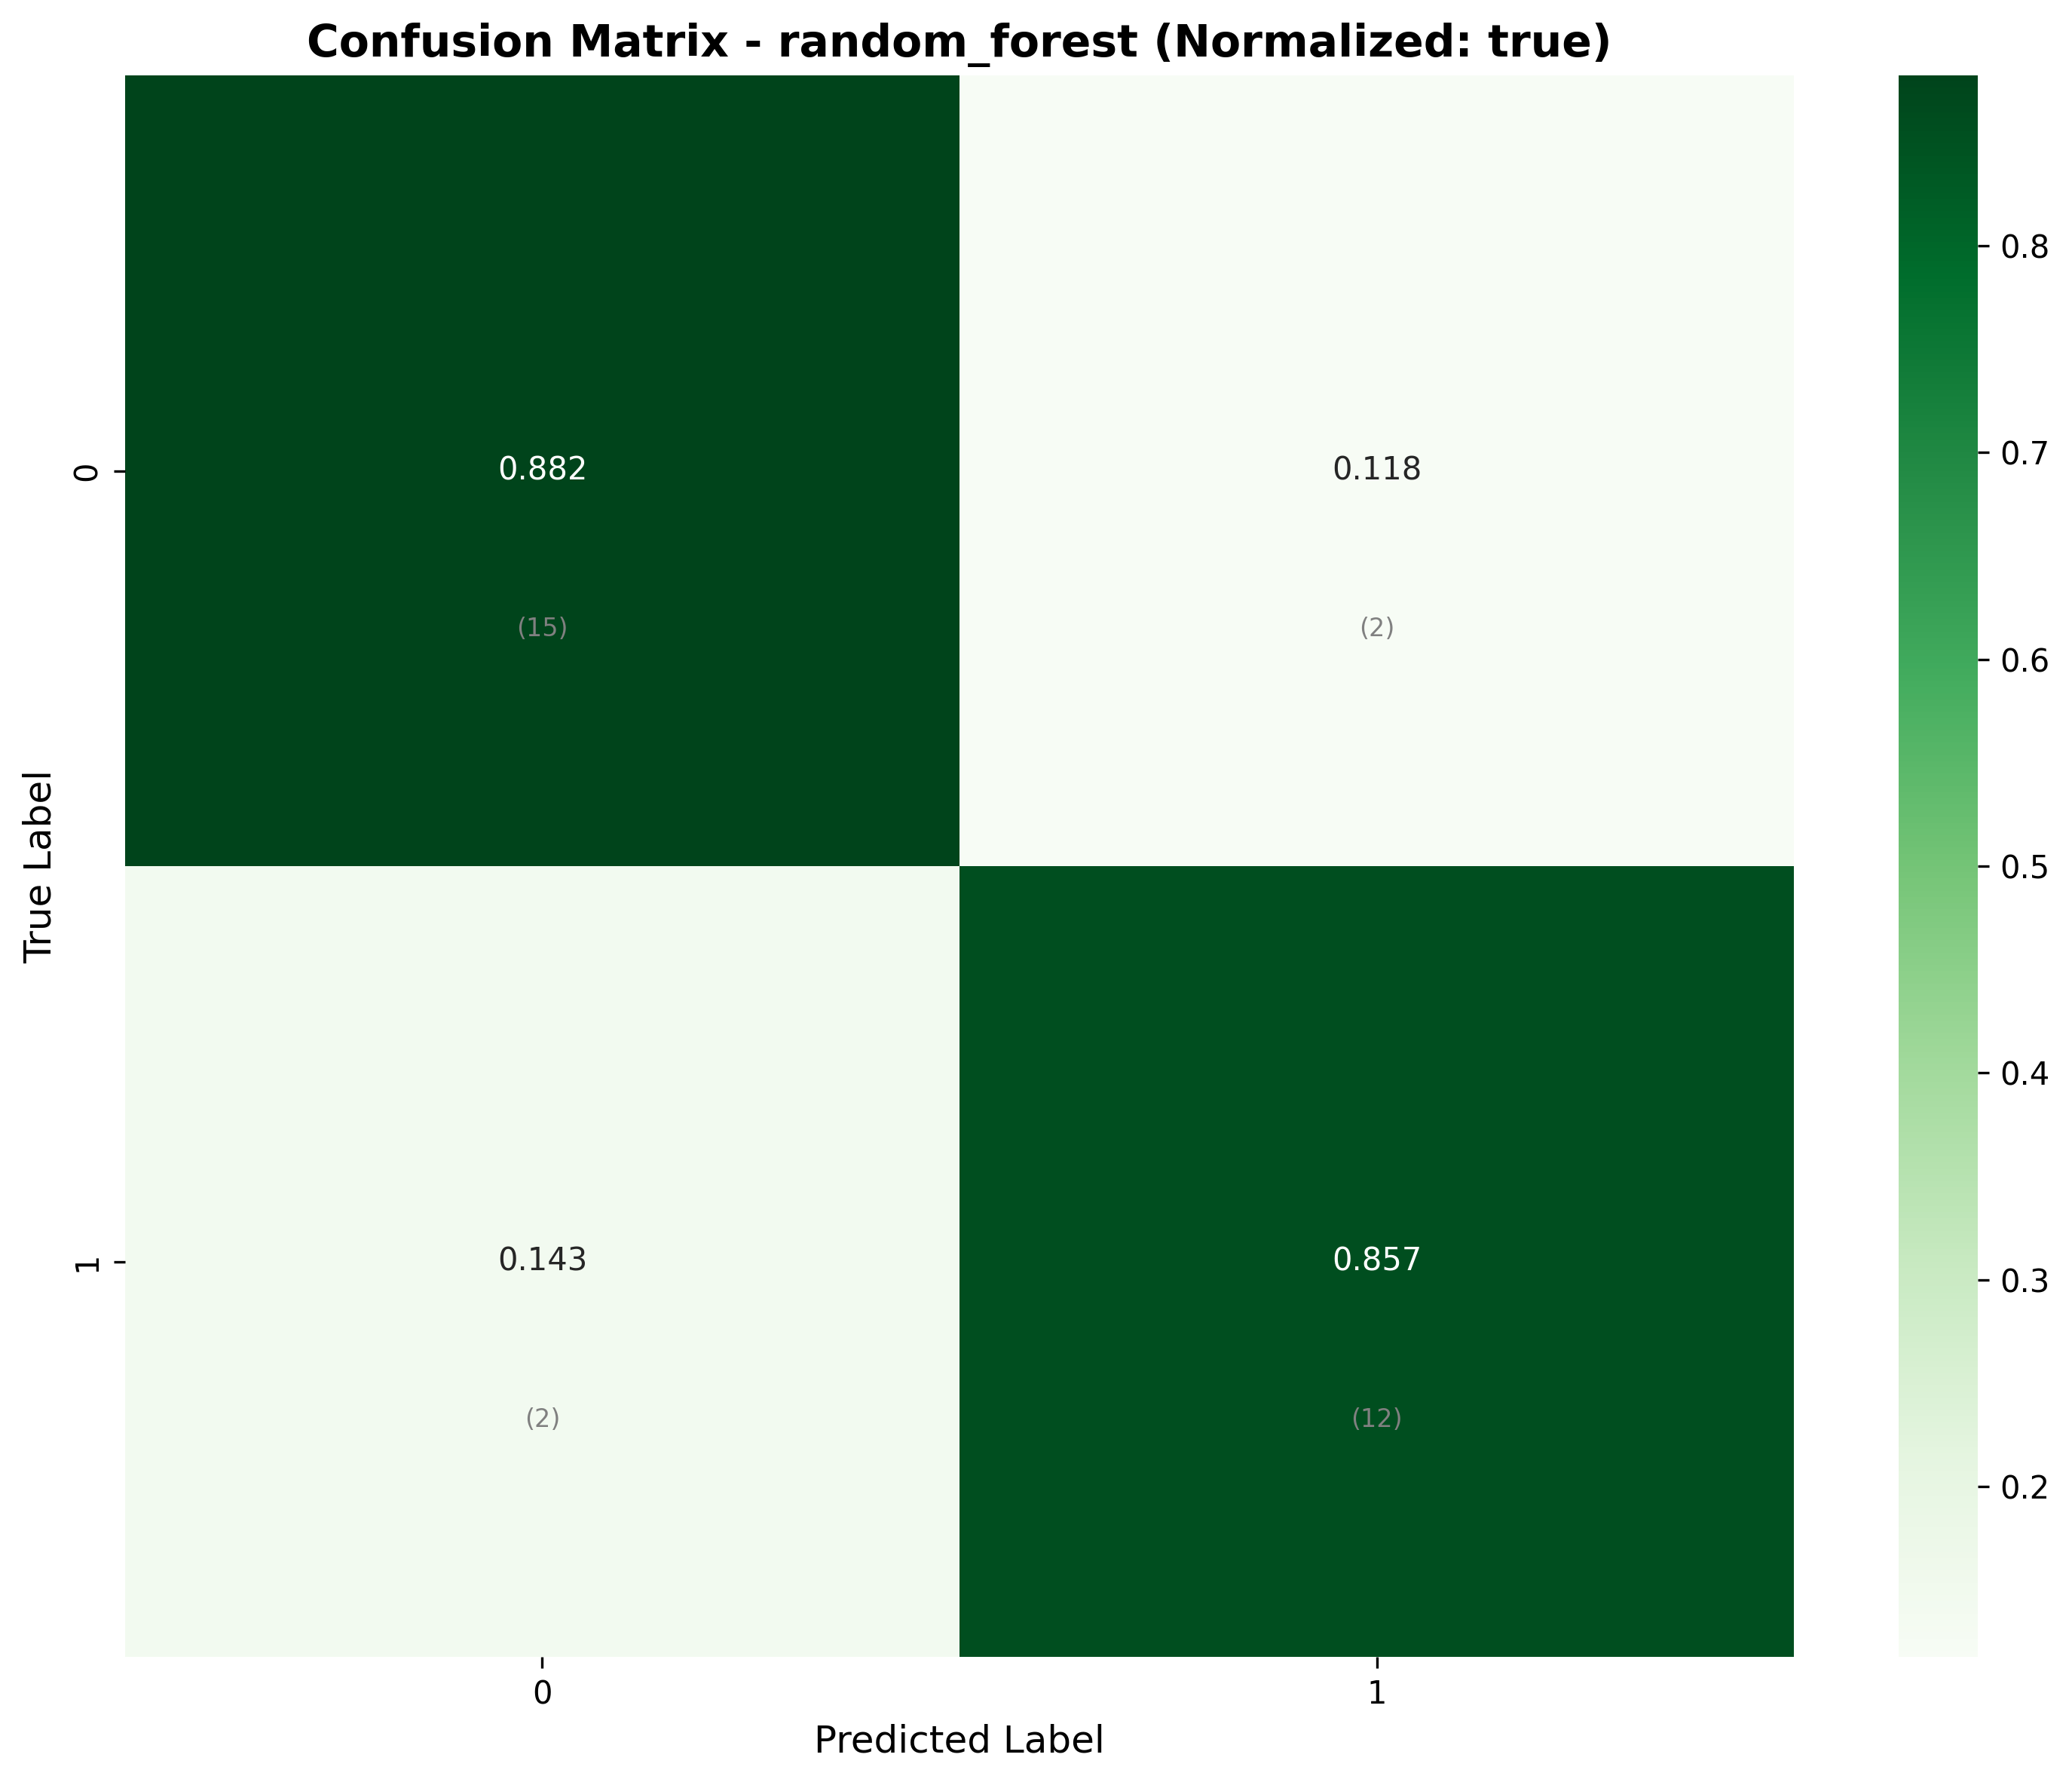
\includegraphics[width=1\textwidth]{Result/cleveland_dataset/confusion_matrices/random_forest_numeric_dataset_RobustScaler.png}
\caption{RF + RobustScaler (87.1\%)}
\label{fig:rf_robustscaler}
\end{subfigure}

\caption{Ma trận Confusion Random Forest với Tất cả Scalers trên Cleveland Dataset. Chứng minh tính nhất quán đáng chú ý với độ chính xác 87.1\% qua tất cả các phương pháp tiền xử lý, xác nhận tính robust của Random Forest với lựa chọn scaling.}
\label{fig:rf_all_scalers_complete}
\end{figure}

Hình \ref{fig:rf_all_scalers_complete} chứng minh tính nhất quán đặc biệt của Random Forest trên tất cả các scalers, duy trì độ chính xác đồng nhất 87.1\% với hiệu suất phân loại cân bằng. Tính robust này xác thực tính hữu ích của RF trong triển khai lâm sàng nơi tính nhất quán tiền xử lý có thể thay đổi.

Random Forest duy trì hiệu suất bất biến qua scalers do cơ chế ensemble với 3 yếu tố chính: Đa dạng hóa thu thập với mỗi cây huấn luyện trên mẫu bootstrap ngẫu nhiên giảm quá khớp đến phân phối đặc trưng cụ thể; Phương pháp không gian ngẫu nhiên với lựa chọn ngẫu nhiên các đặc trưng tại mỗi phân chia tạo khả năng kháng với độ nhạy scaling điểm đơn; Tập hợp bỏ phiếu đa số khi cuối cùng đầu ra là trung bình của nhiều predictors đa dạng, tự nhiên làm mượt các biến đổi phụ thuộc phân phối. Điều này làm RF lý tưởng cho các hệ thống lâm sàng nơi pipelines tiền xử lý dữ liệu có thể thay đổi qua các tổ chức hoặc phát triển theo thời gian mà không cần huấn luyện lại mô hình.

\subsubsection{Decision Tree - Scalability Analysis}

\begin{figure}[H]
\centering
\begin{subfigure}[b]{0.315\textwidth}
\centering
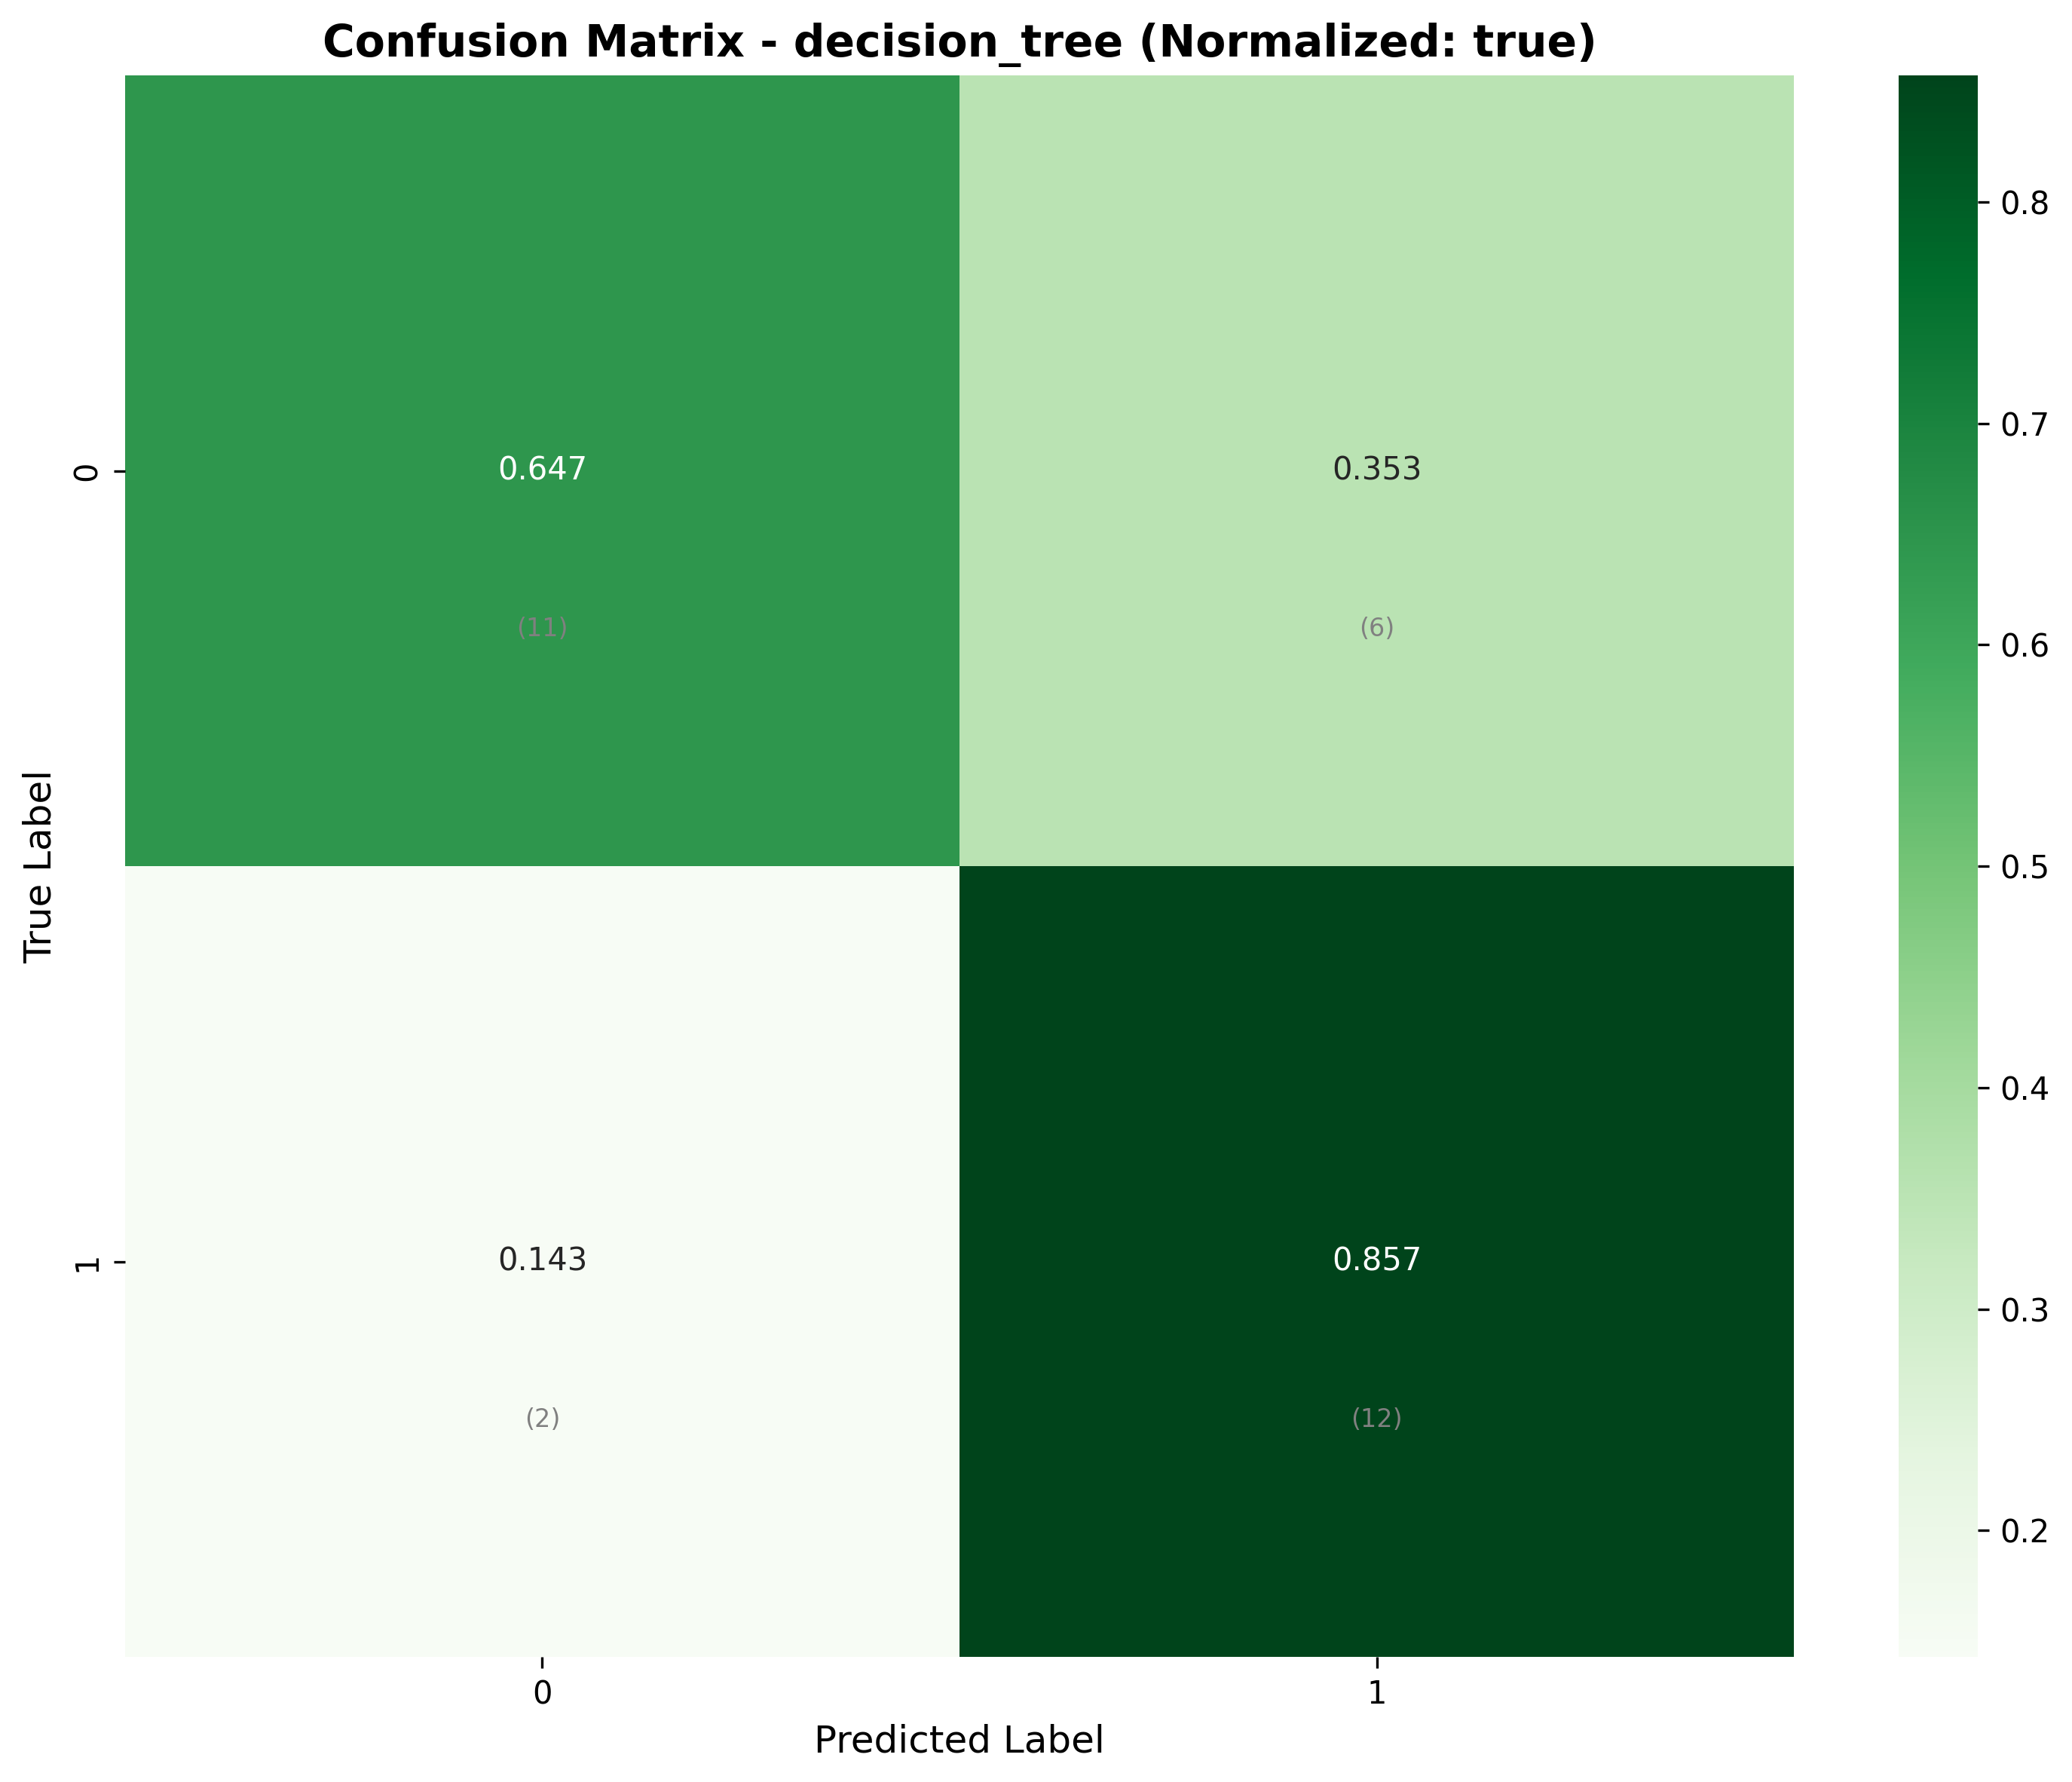
\includegraphics[width=1\textwidth]{Result/cleveland_dataset/confusion_matrices/decision_tree_numeric_dataset_StandardScaler.png}
\caption{DT + StandardScaler (74.2\%)}
\label{fig:dt_standardscaler}
\end{subfigure}
\hfill
\begin{subfigure}[b]{0.315\textwidth}
\centering
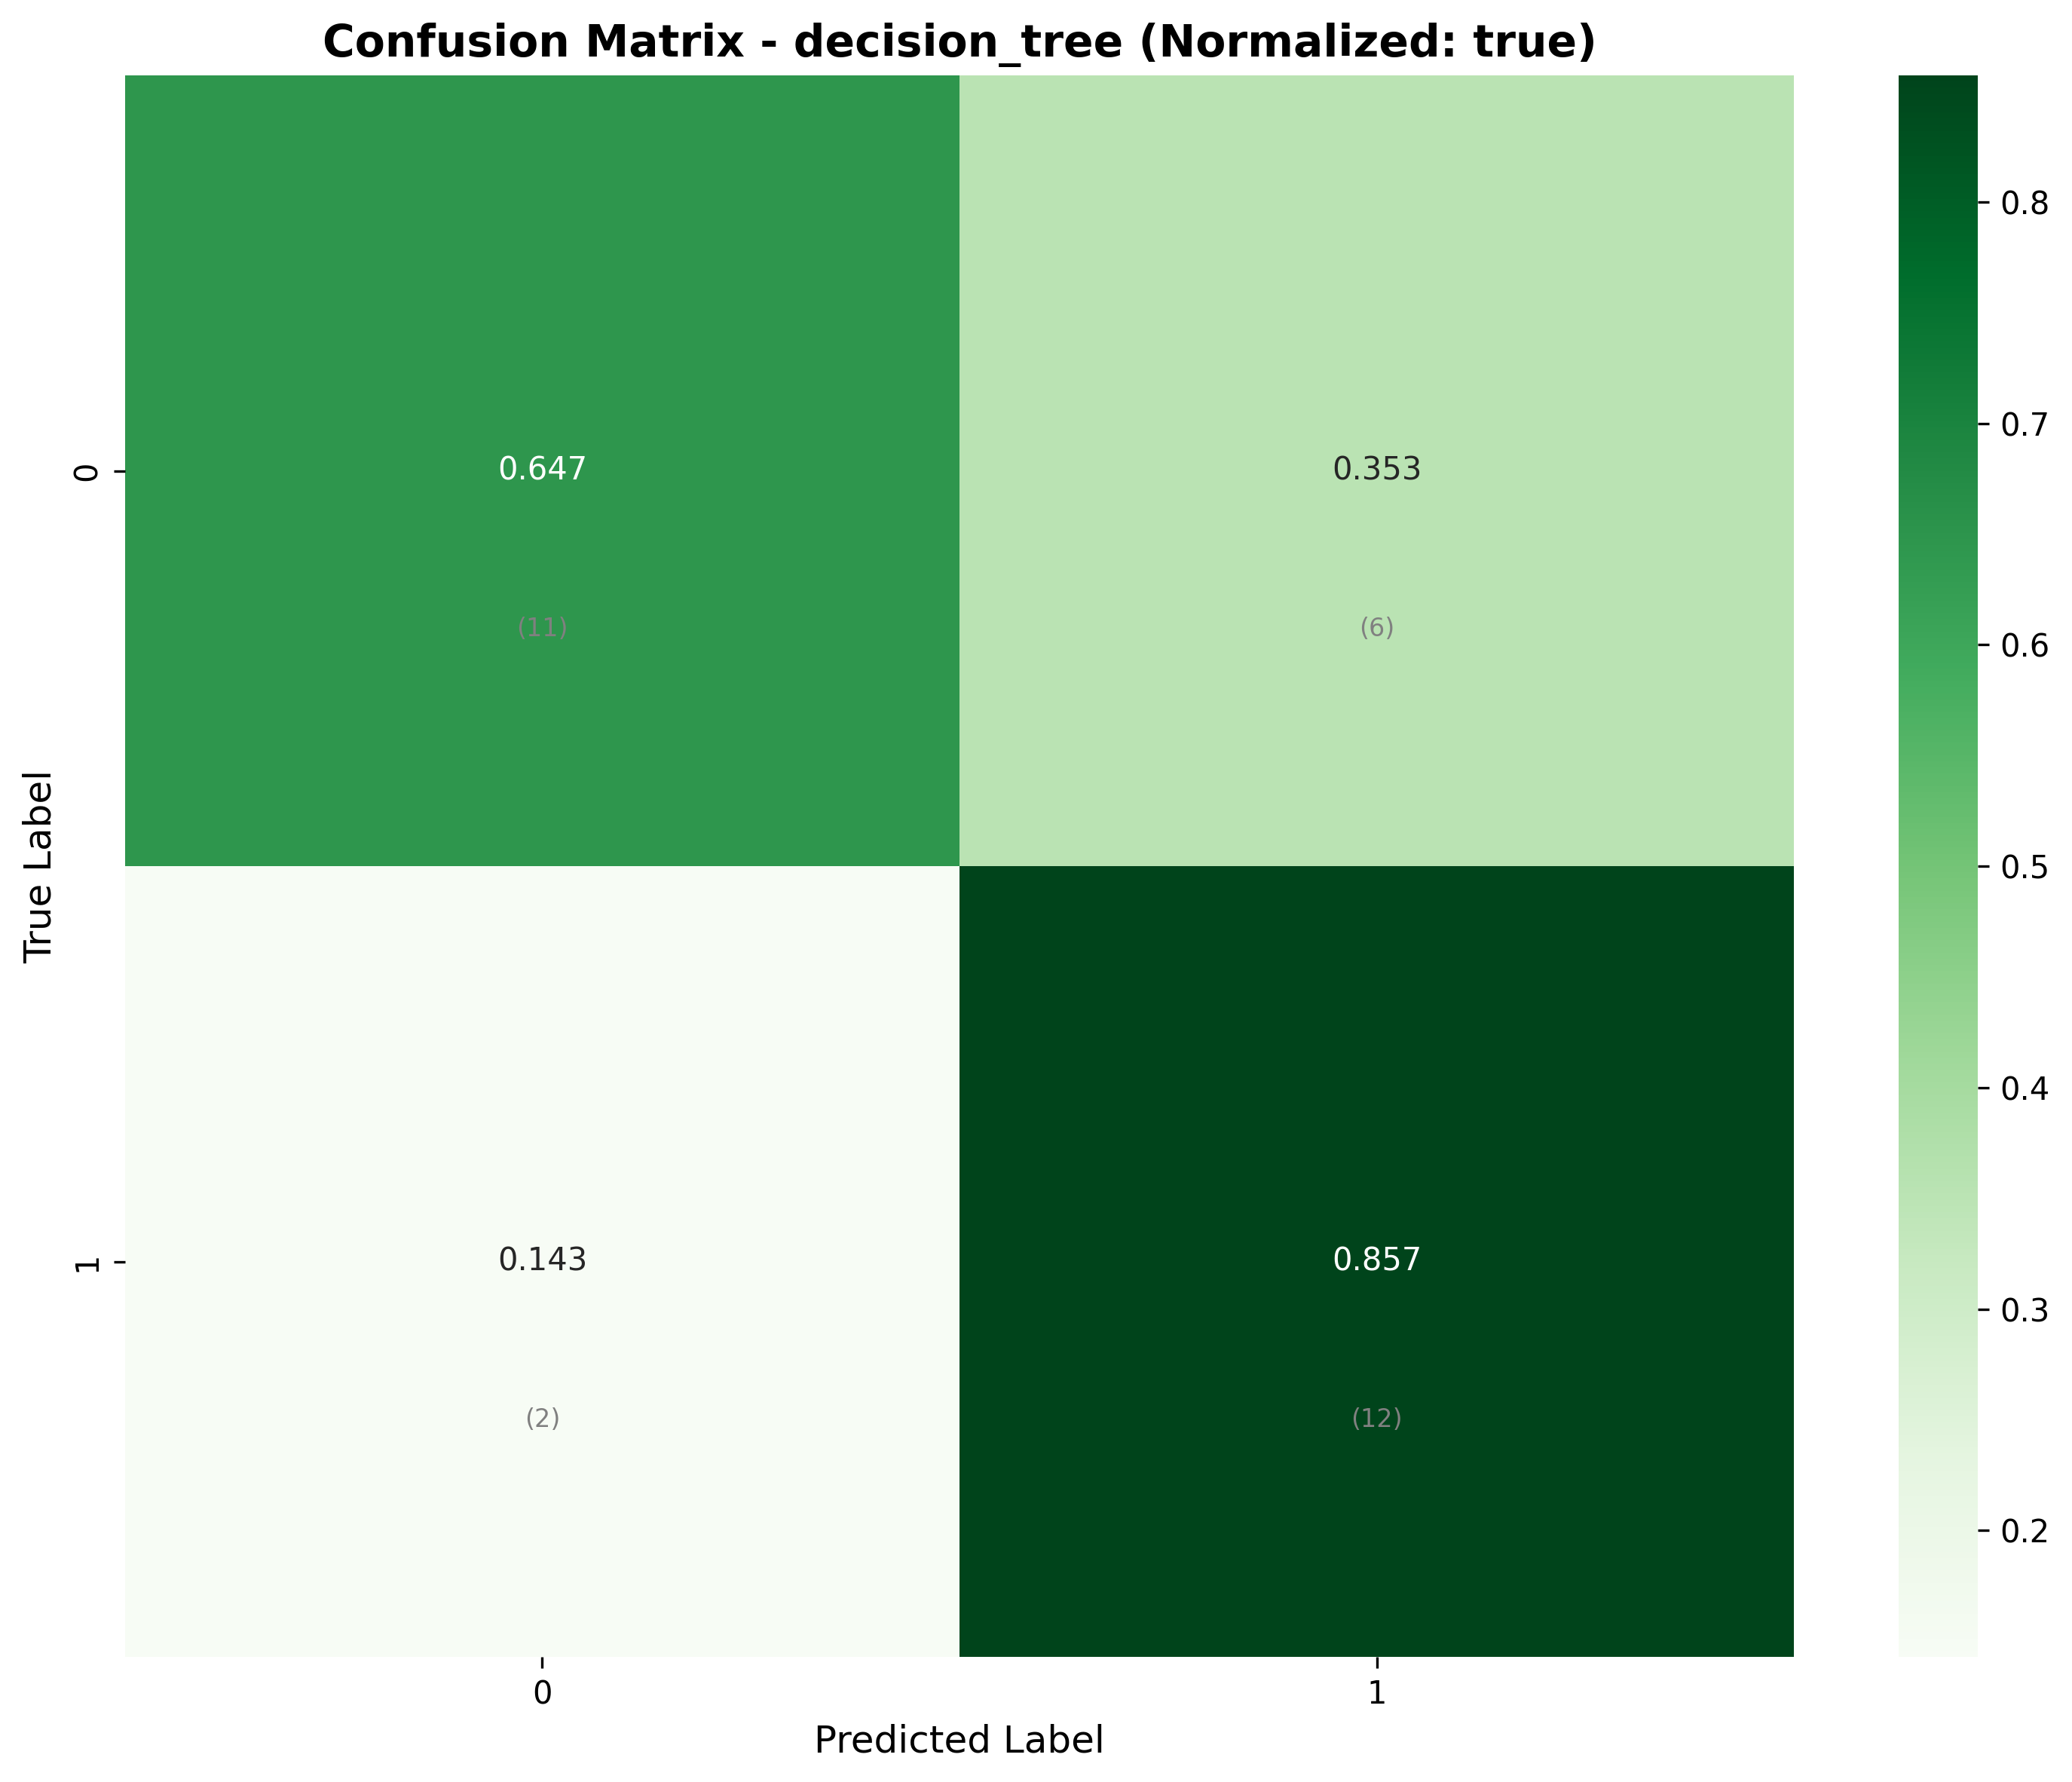
\includegraphics[width=1\textwidth]{Result/cleveland_dataset/confusion_matrices/decision_tree_numeric_dataset_MinMaxScaler.png}
\caption{DT + MinMaxScaler (74.2\%)}
\label{fig:dt_minmaxscaler}
\end{subfigure}
\hfill
\begin{subfigure}[b]{0.315\textwidth}
\centering
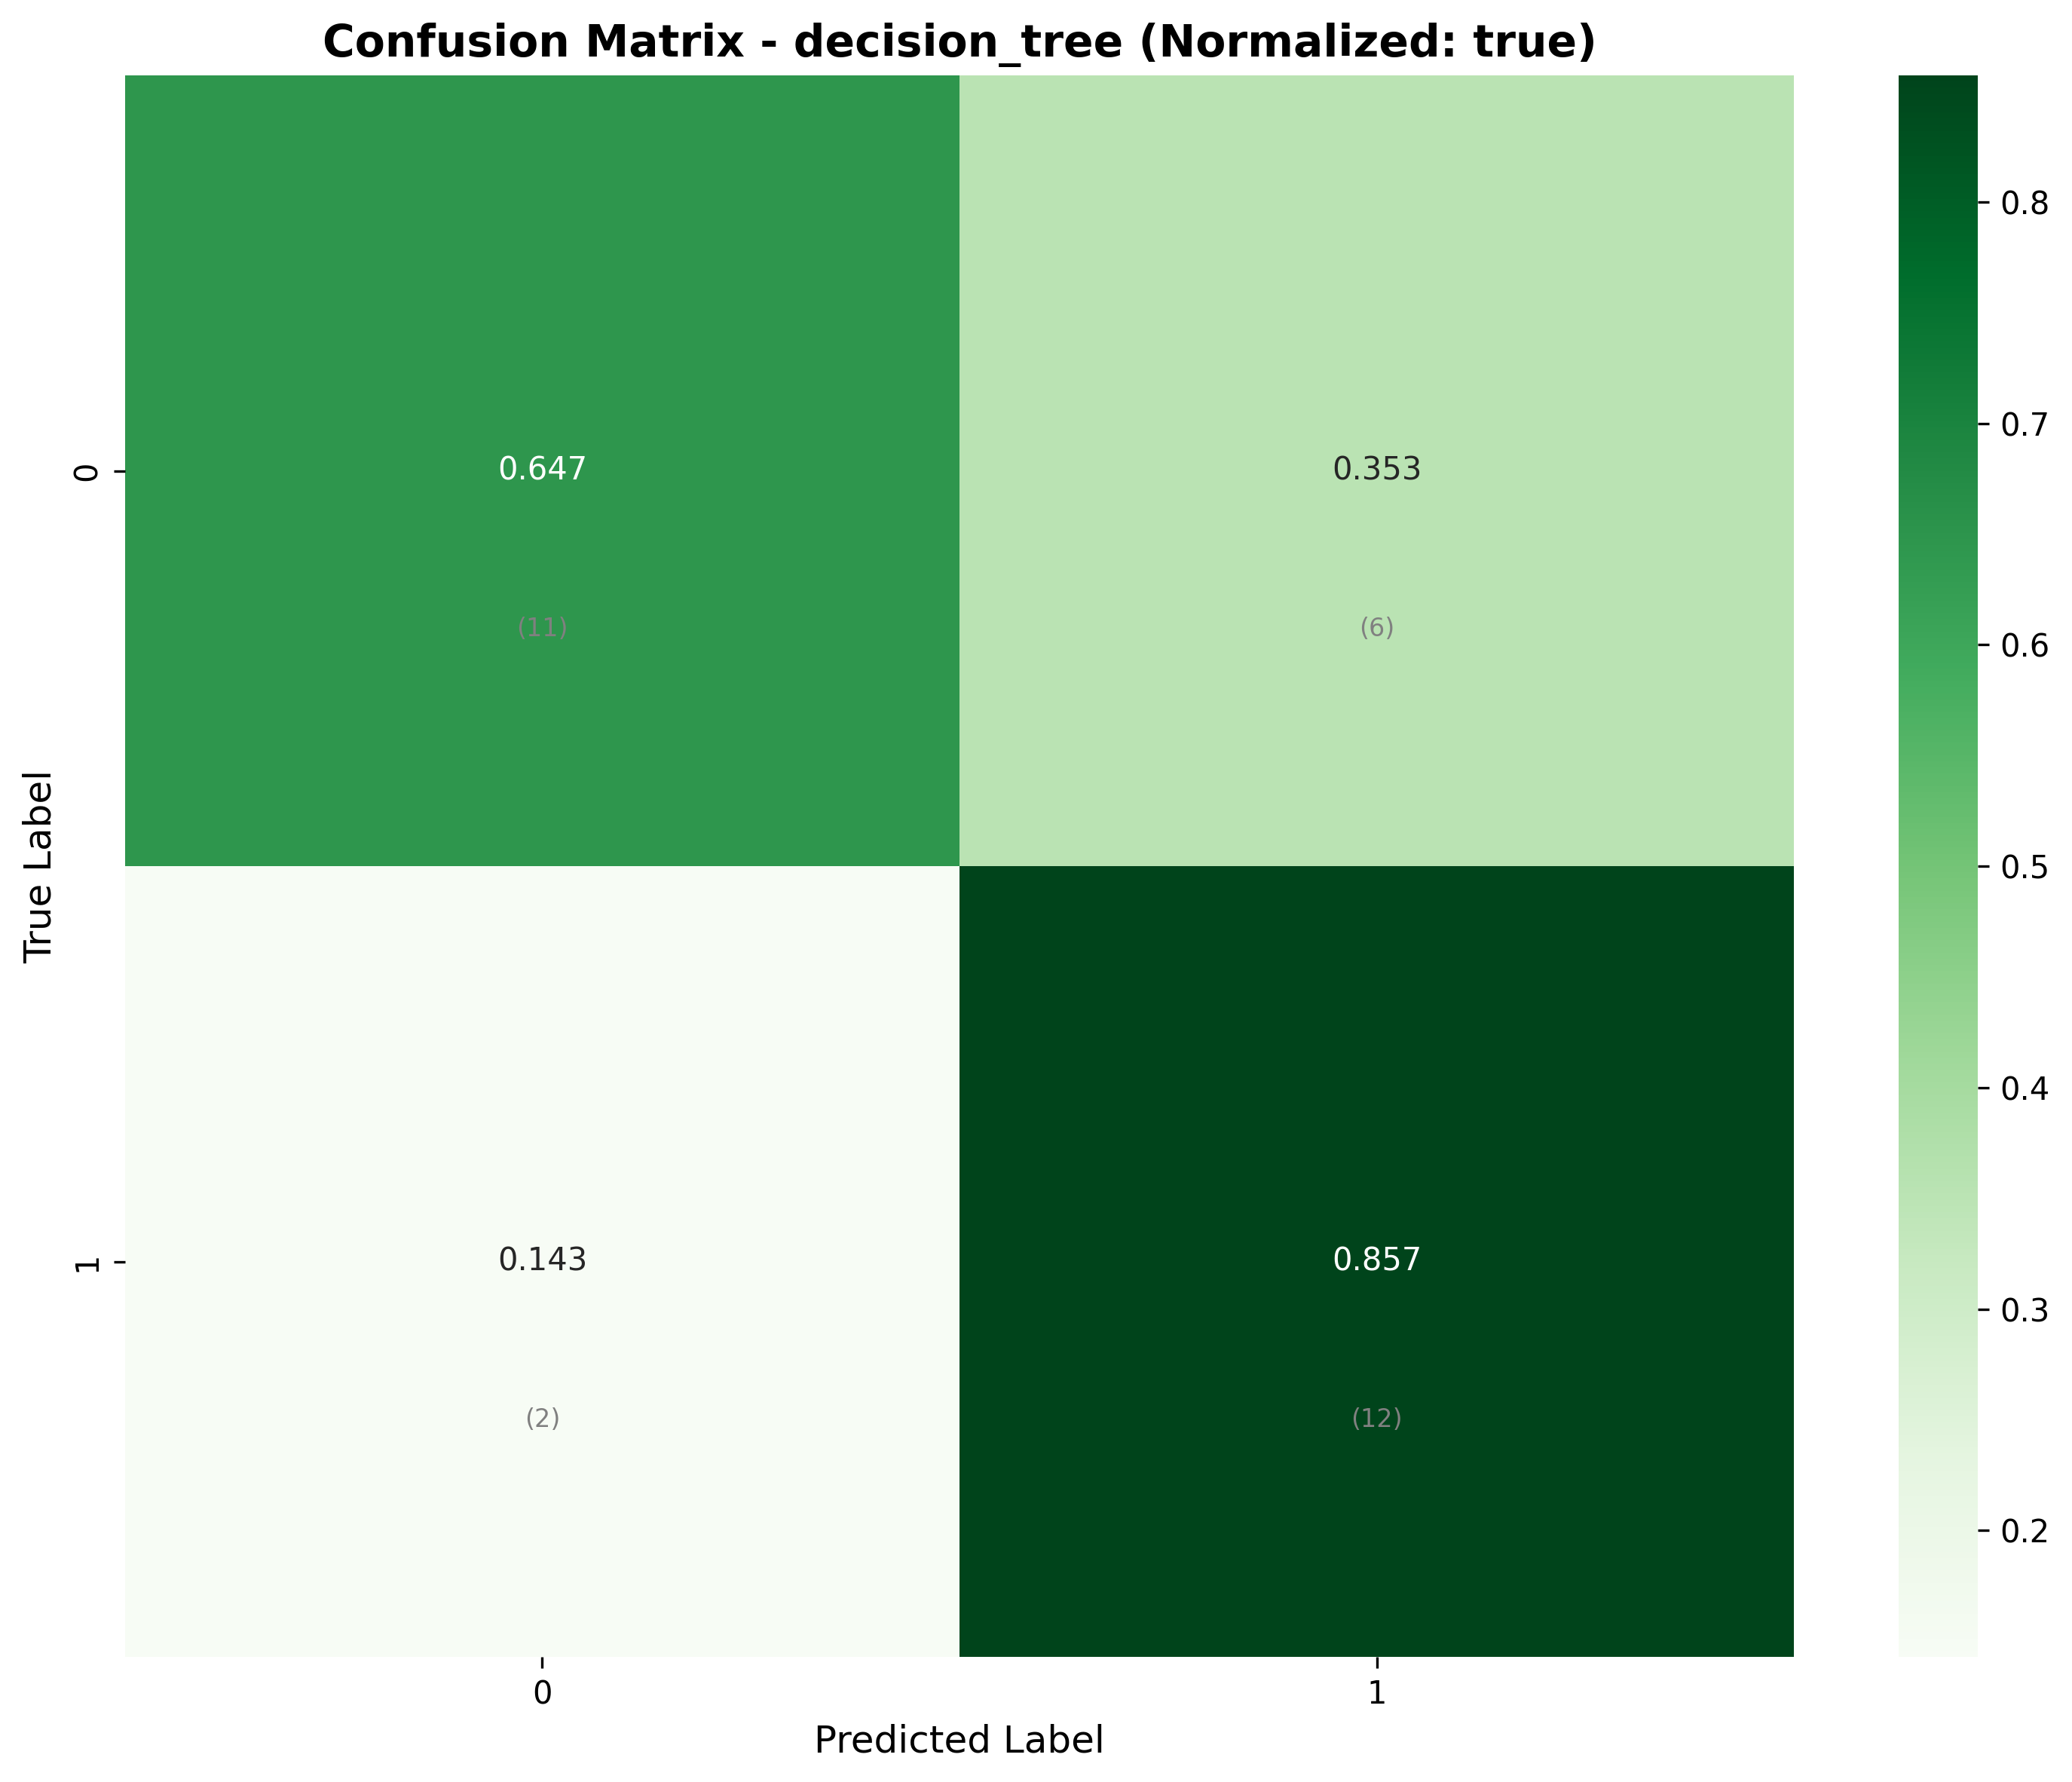
\includegraphics[width=1\textwidth]{Result/cleveland_dataset/confusion_matrices/decision_tree_numeric_dataset_RobustScaler.png}
\caption{DT + RobustScaler (74.2\%)}

\label{fig:dt_robustscaler}
\end{subfigure}

\caption{Ma trận Confusion Decision Tree với Tất cả Scalers trên Cleveland Dataset. Độ chính xác nhất quán 74.2\% chứng minh tính độc lập tiền xử lý của DT, mặc dù hiệu suất tổng thể thấp hơn cho thấy các hạn chế của cây đơn lẻ.}
\label{fig:dt_all_scalers}
\end{figure}

Hiệu suất Decision Tree cho thấy tính nhất quán với độ chính xác 74.2\% trên các scalers, xác nhận tính độc lập của các thuật toán cây đơn lẻ đối với feature scaling. Hiệu suất thấp hơn nhấn mạnh tầm quan trọng của các phương pháp ensemble trong việc đạt được độ chính xác cấp lâm sàng.

Hiệu suất Decision Tree đạt đỉnh tại 74.2\% do các hạn chế cơ bản của thuật toán greedy splitting. Vấn đề Tối ưu cục bộ khi cây sử dụng quyết định tham lam tại mỗi nút mà không xem xét các phân chia tối ưu toàn cục, dẫn đến ngưỡng đặc trưng tối ưu phụ; Phương sai cao với các thay đổi nhỏ trong dữ liệu huấn luyện có thể thay đổi cấu trúc cây đáng kể do độ nhạy với các mẫu cá nhân; Rủi ro quá khớp khi cây có thể phát triển đủ sâu để ghi nhớ các mẫu huấn luyện mà không tổng quát hóa tốt với dữ liệu kiểm tra; Tính độc lập Scaler với tính liên quan hạn chế vì cây phân chia dựa trên thứ hạng tương đối của đặc trưng, làm chúng không nhạy cảm với các biến đổi tuyến tính nhưng dễ bị tổn thương với các thay đổi phân phối tinh tế hơn. Phân tích này chứng minh các phương pháp ensemble như Random Forest mà tổng hợp nhiều cây để giảm phương sai và cải thiện hiệu suất tổng quát hóa.

\subsection{Phân tích Toàn diện Các Mô hình Khác}

\subsubsection{Mô hình Tuyến tính - SVM và Logistic Regression}

\begin{figure}[H]
\centering
\begin{subfigure}[b]{0.315\textwidth}
\centering
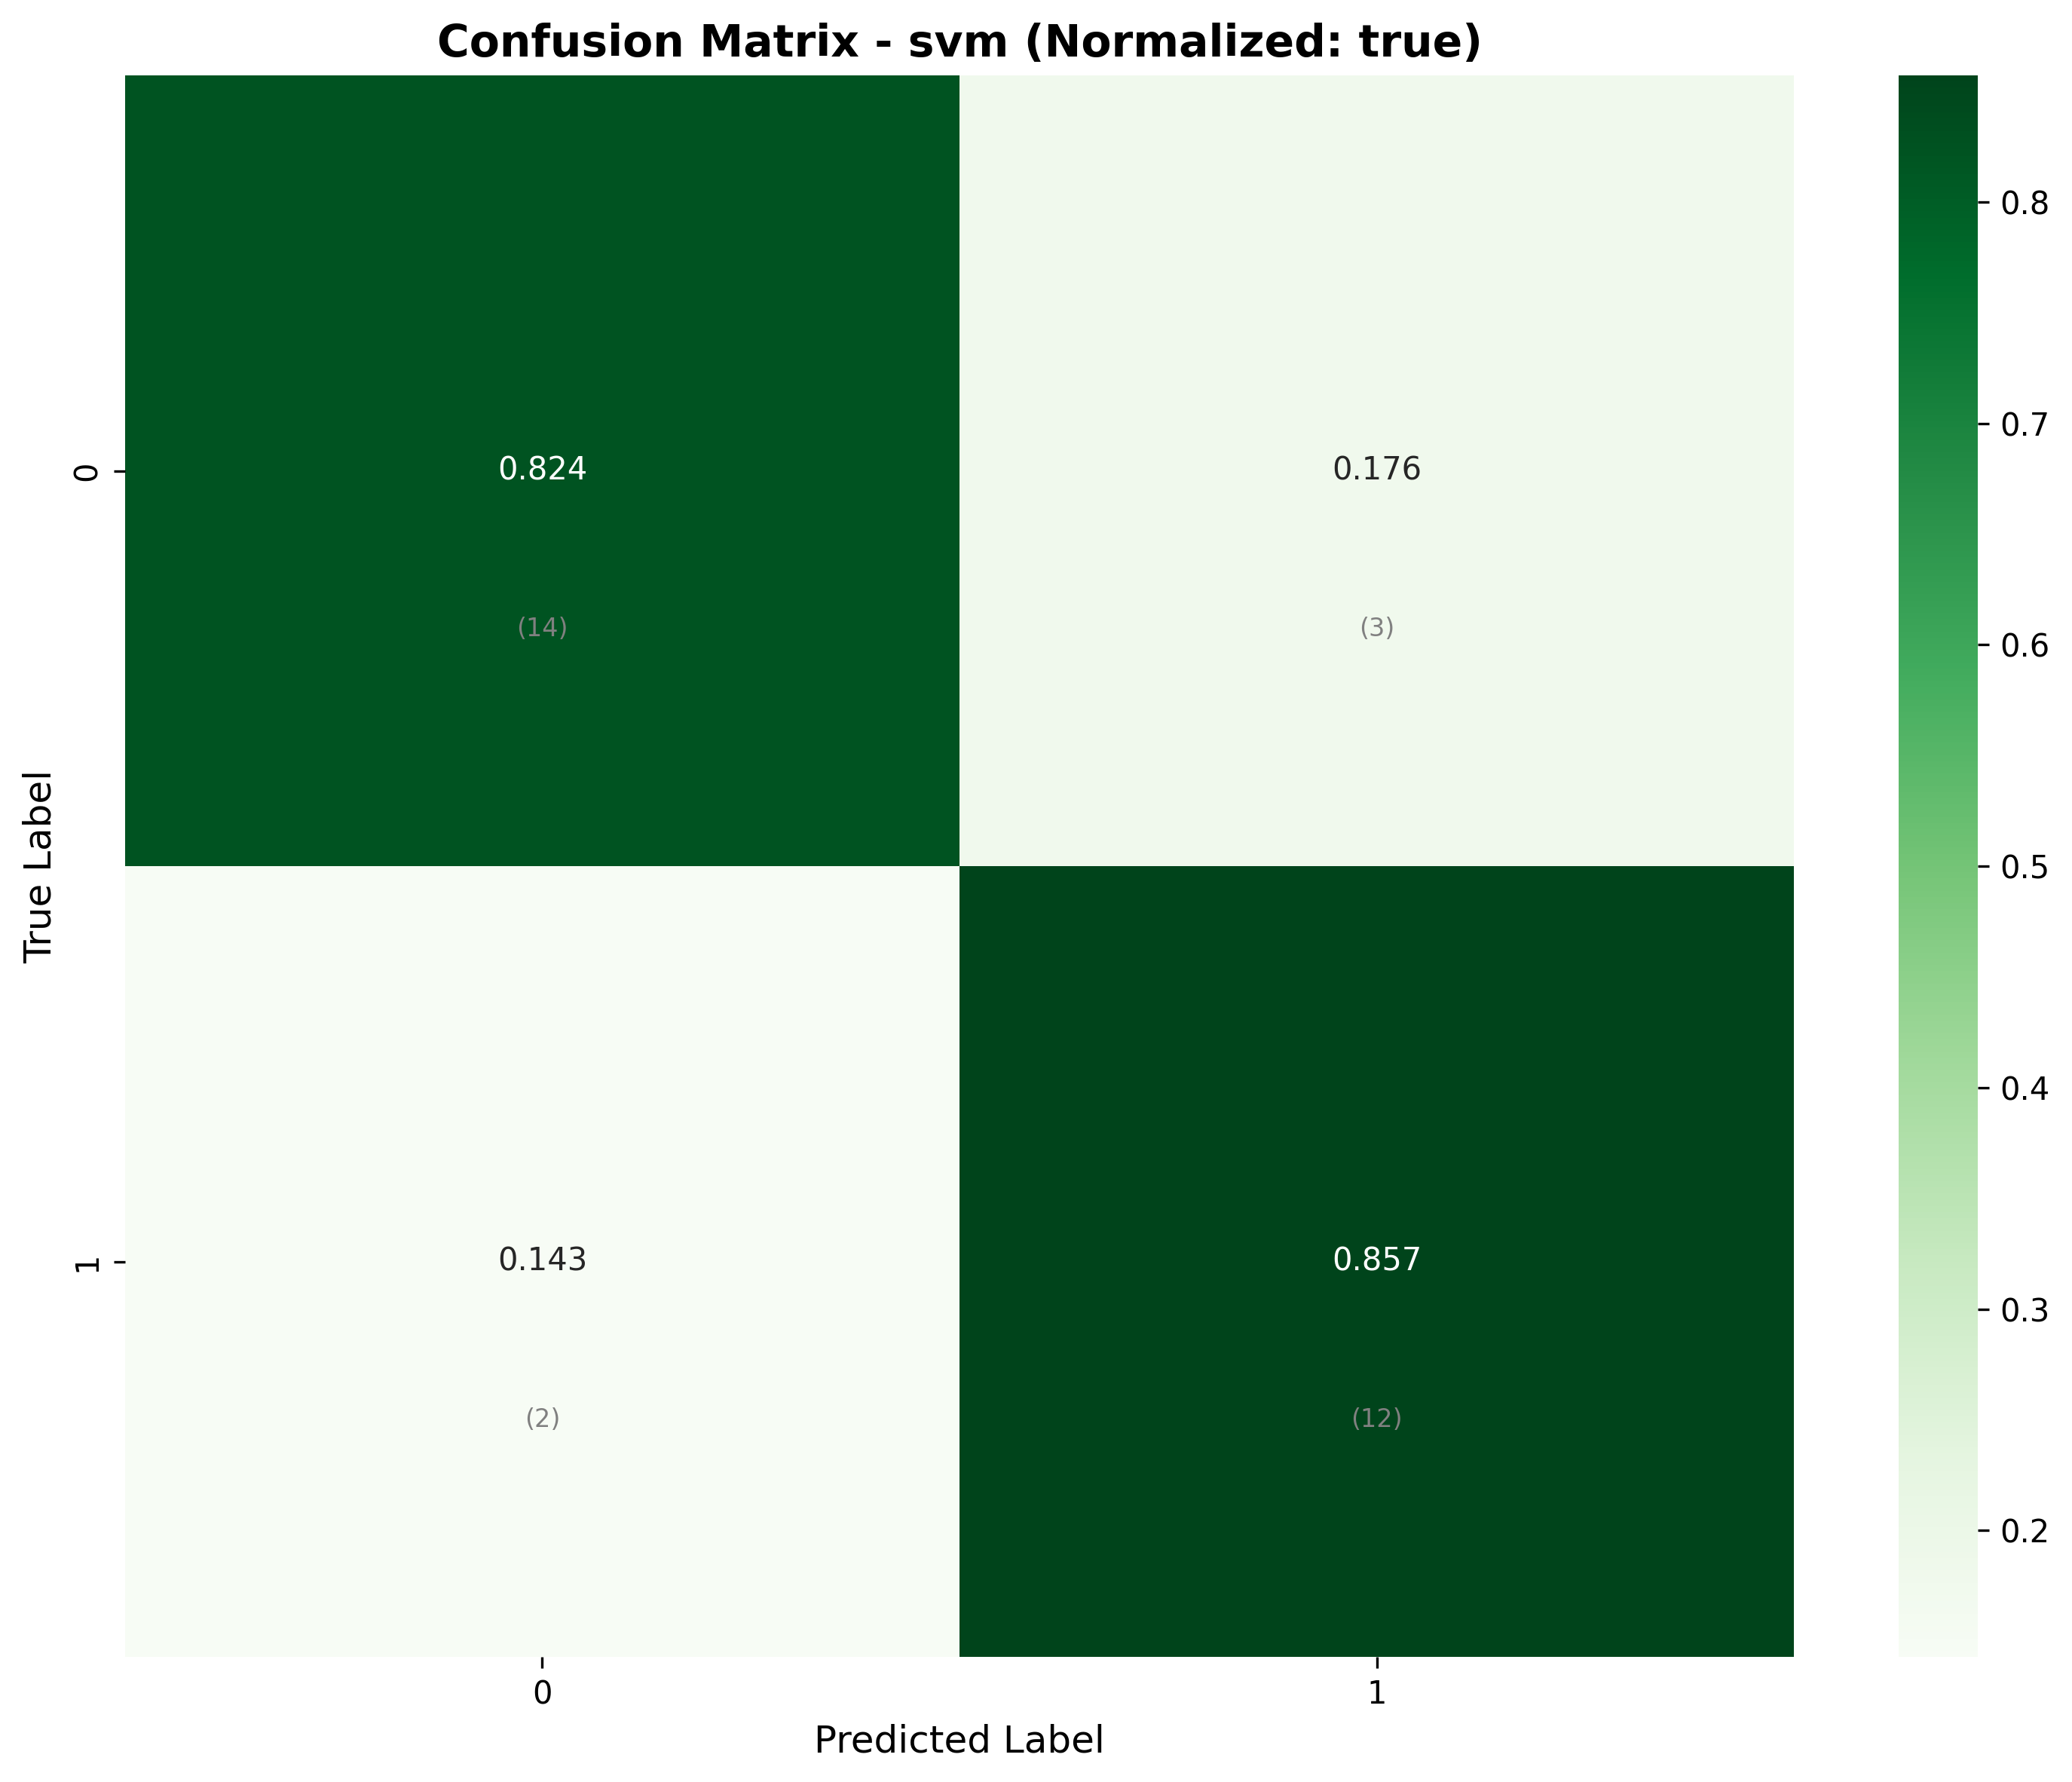
\includegraphics[width=1\textwidth]{Result/cleveland_dataset/confusion_matrices/svm_numeric_dataset_StandardScaler.png}
\caption{SVM + StandardScaler (83.9\%)}
\label{fig:svm_standardscaler_complete}
\end{subfigure}
\hfill
\begin{subfigure}[b]{0.315\textwidth}
\centering
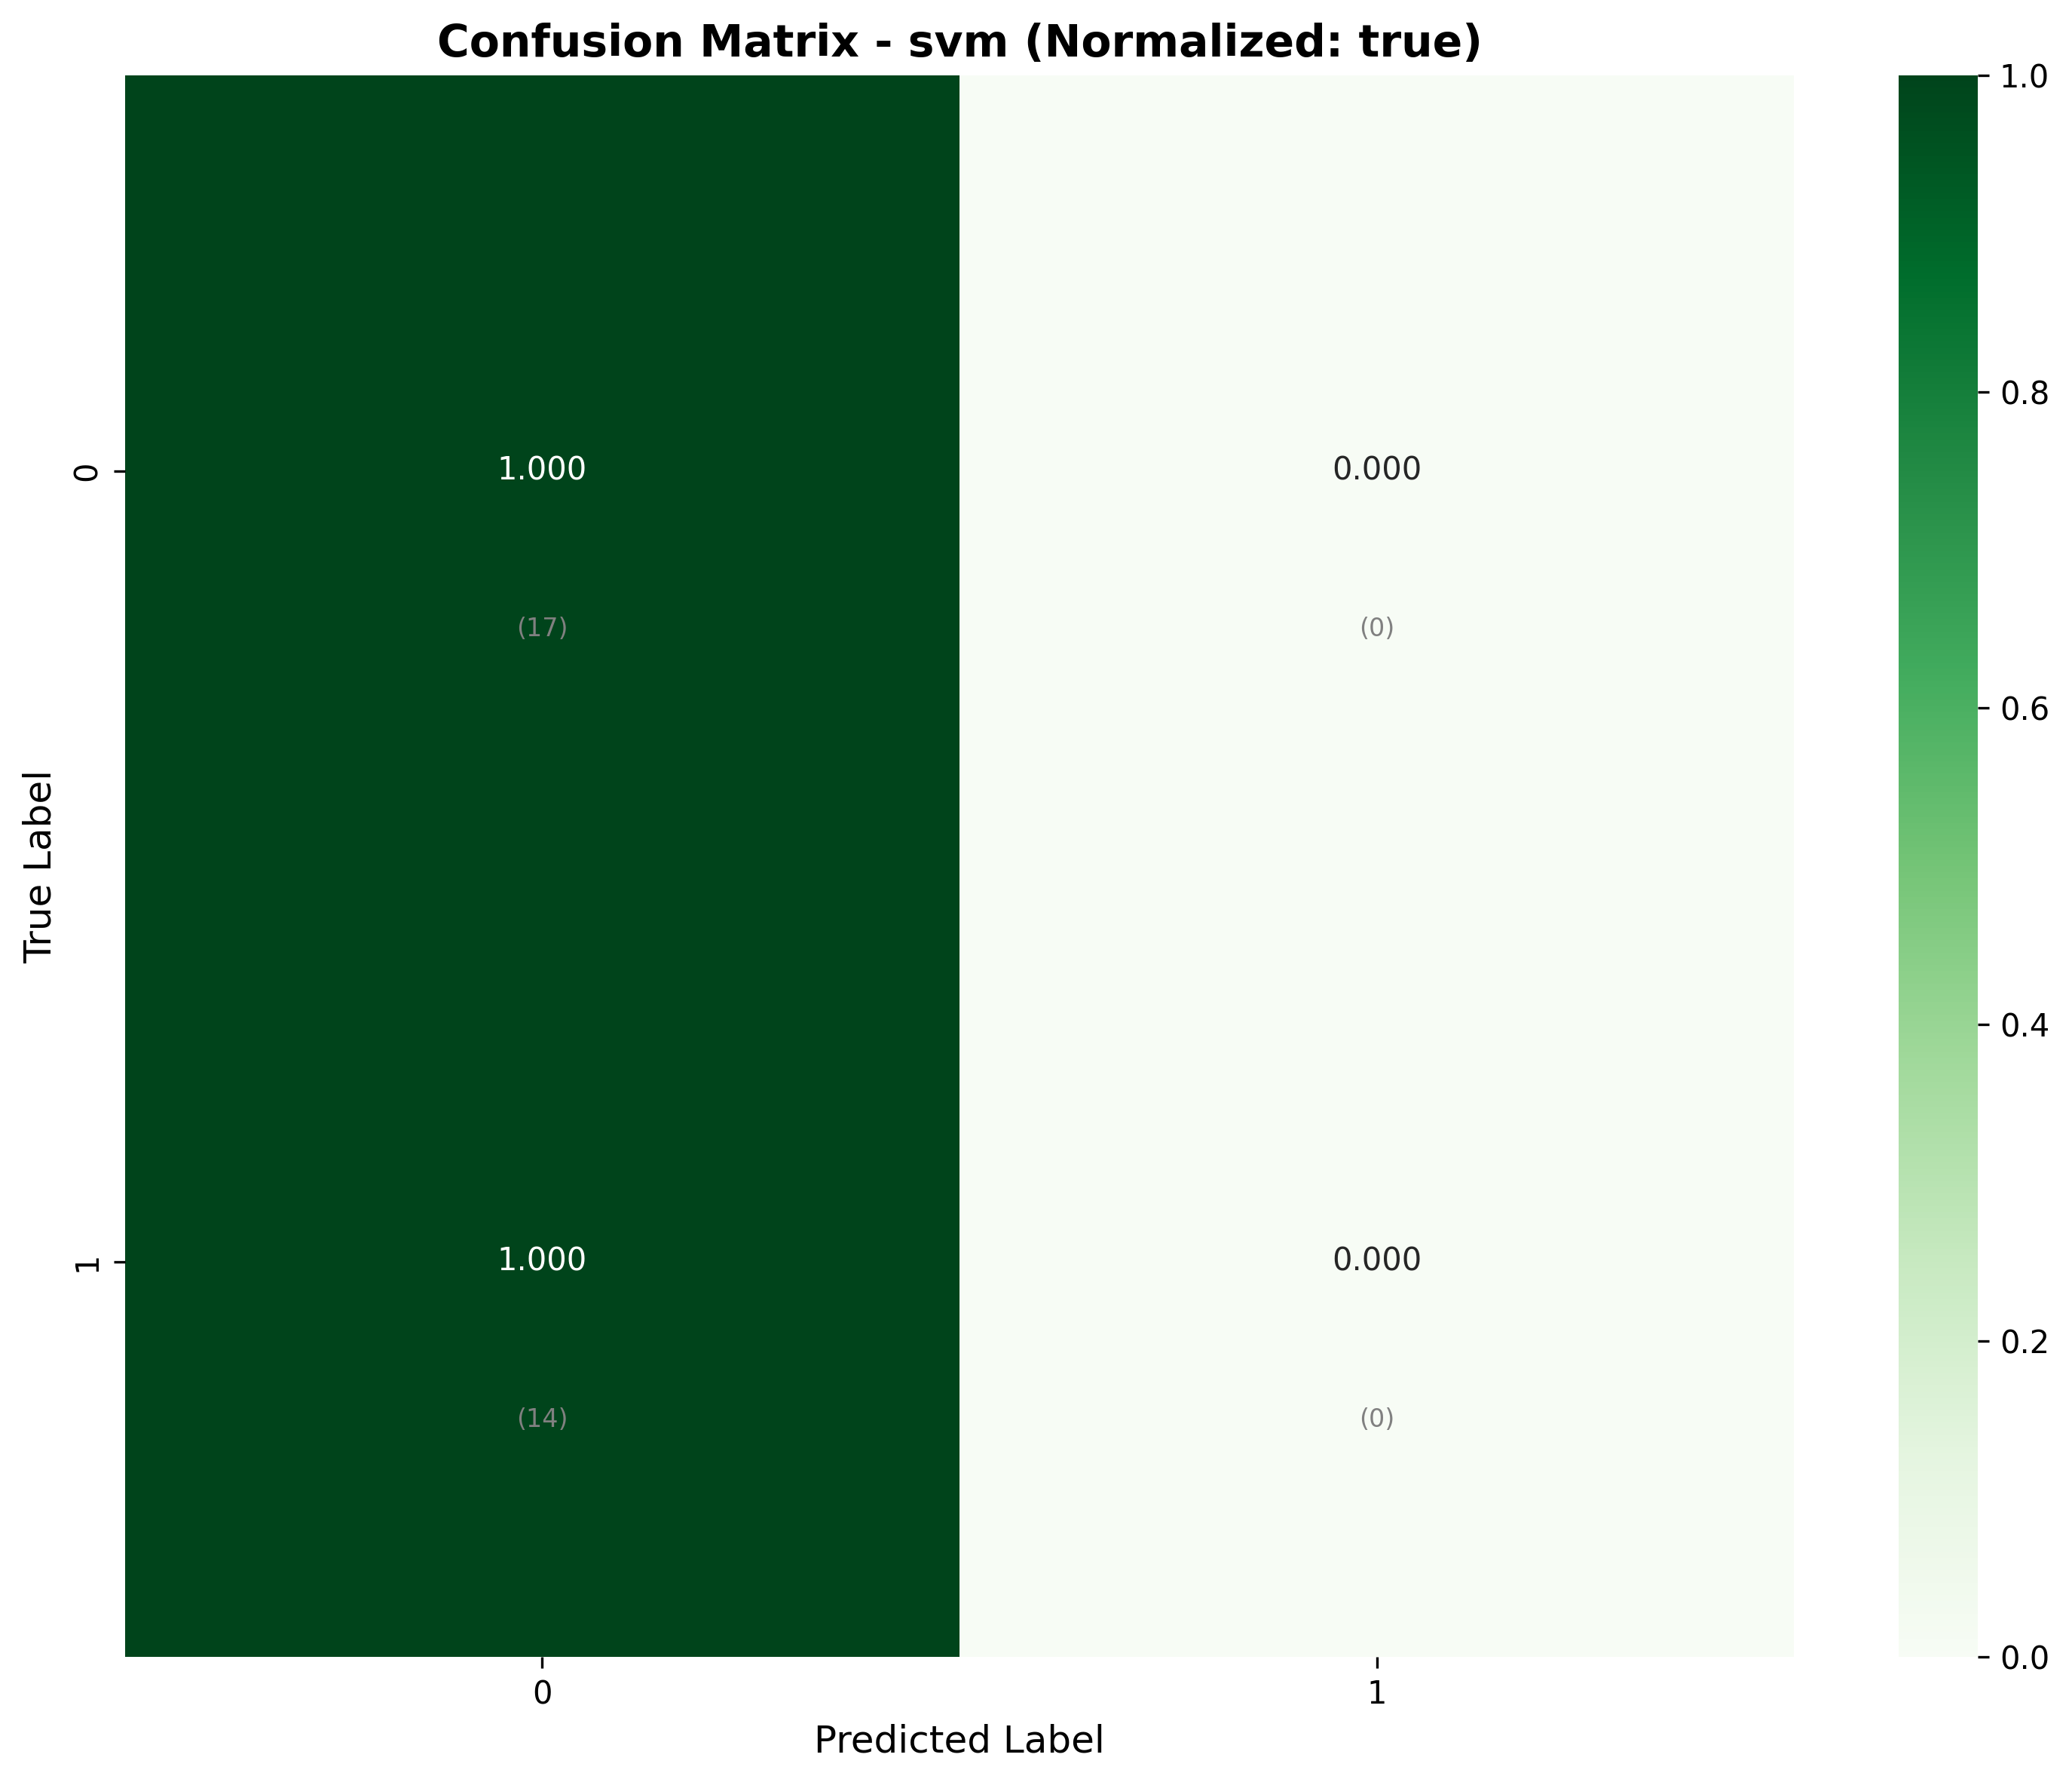
\includegraphics[width=1\textwidth]{Result/cleveland_dataset/confusion_matrices/svm_numeric_dataset_MinMaxScaler.png}
\caption{SVM + MinMaxScaler (54.8\%)}
\label{fig:svm_minmaxscaler_complete}
\end{subfigure}
\hfill
\begin{subfigure}[b]{0.315\textwidth}
\centering
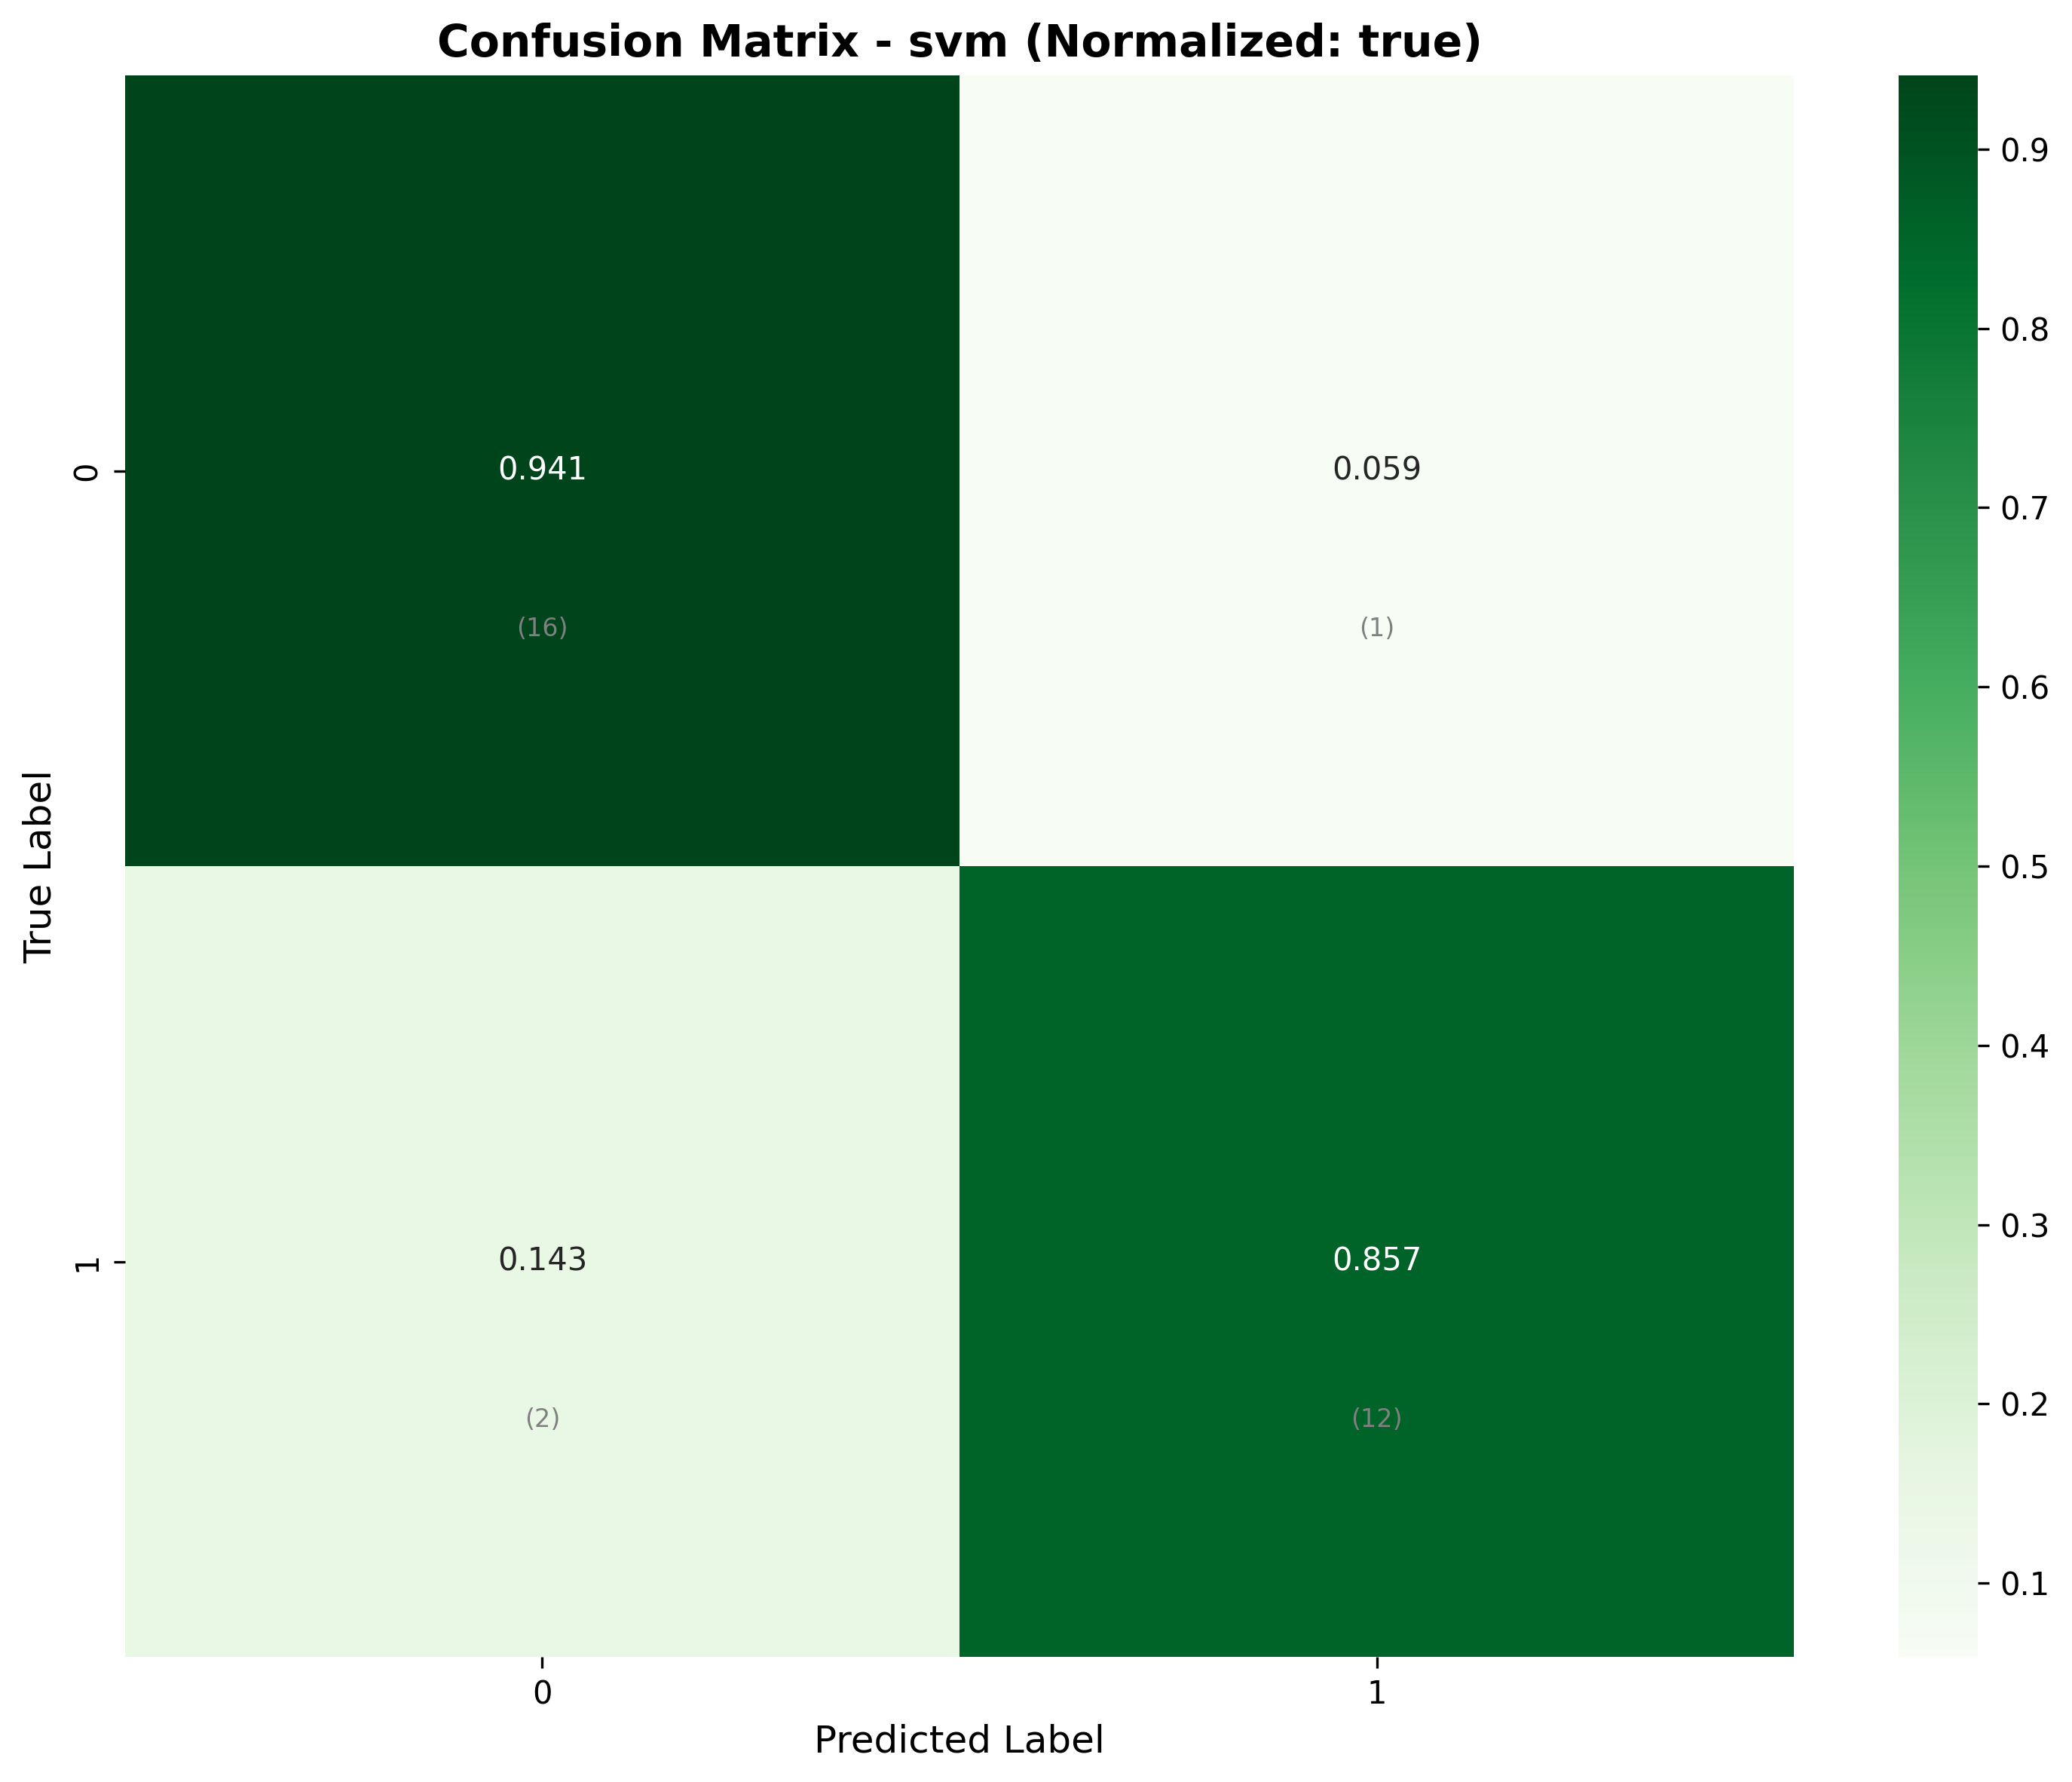
\includegraphics[width=1\textwidth]{Result/cleveland_dataset/confusion_matrices/svm_numeric_dataset_RobustScaler.png}
\caption{SVM + RobustScaler (90.3\%)}
\label{fig:svm_robustscaler_complete}
\end{subfigure}

\caption{SVM Confusion Matrices Complete Set trên Cleveland Dataset. Demonstrates extreme scaler sensitivity từ 54.8\% (MinMaxScaler) đến 90.3\% (RobustScaler), highlighting critical importance của preprocessing choice cho linear algorithms trong clinical applications.}
\label{fig:svm_all_scalers_complete_analysis}
\end{figure}

Figures \ref{fig:svm_standardscaler_complete}-\ref{fig:svm_robustscaler_complete} thể hiện dramatic scaler sensitivity của SVM, với performance thay đổi đáng kể từ 54.8\% đến 90.3\%. Điều này xác thực RobustScaler enabling optimal SVM performance với proper outlier handling tại medical datasets.

Biến thiên hiệu suất SVM (54.8\% MinMaxScaler vs 90.3\% RobustScaler) phản ánh các thuộc tính toán học cơ bản của tính toán support vector. Tối ưu hóa Biên hình học khi SVM tìm siêu mặt tách biệt tối ưu bằng cách tối đa hóa biên giữa các lớp, làm kết quả cực kỳ nhạy cảm với việc scale đặc trưng ảnh hưởng đến tính toán khoảng cách; Tác động ngoại lệ với MinMaxScaler ép các đặc trưng vào khoảng [0,1] nhưng bảo toàn vị trí ngoại lệ tương đối, thiên vị tính toán biên khi các giá trị cholesterol cực trị hoặc chỉ số huyết áp tạo ra sự tách biệt nhân tạo; Lợi thế RobustScaler sử dụng trung vị và khoảng tứ phân thay vì trung bình/phương sai để giảm ảnh hưởng ngoại lệ và bảo toàn phân phối đặc trưng tự nhiên thiết yếu cho giải thích lâm sàng; Khoảng cách cảm ứng hạt nhân trong không gian đặc trưng đa chiều của dữ liệu tim mạch, việc scale xác định khoảng cách hiệu dụng giữa support vectors và ranh giới quyết định, tác động trực tiếp đến độ chính xác phân loại. Điều này nhấn mạnh tầm quan trọng cực kỳ của tiền xử lý nhận thức miền trong các ứng dụng ML y tế.

\subsubsection{Mô hình Dựa Tri thức - KNN và Naive Bayes}

\begin{figure}[H]
\centering
\begin{subfigure}[b]{0.315\textwidth}
\centering
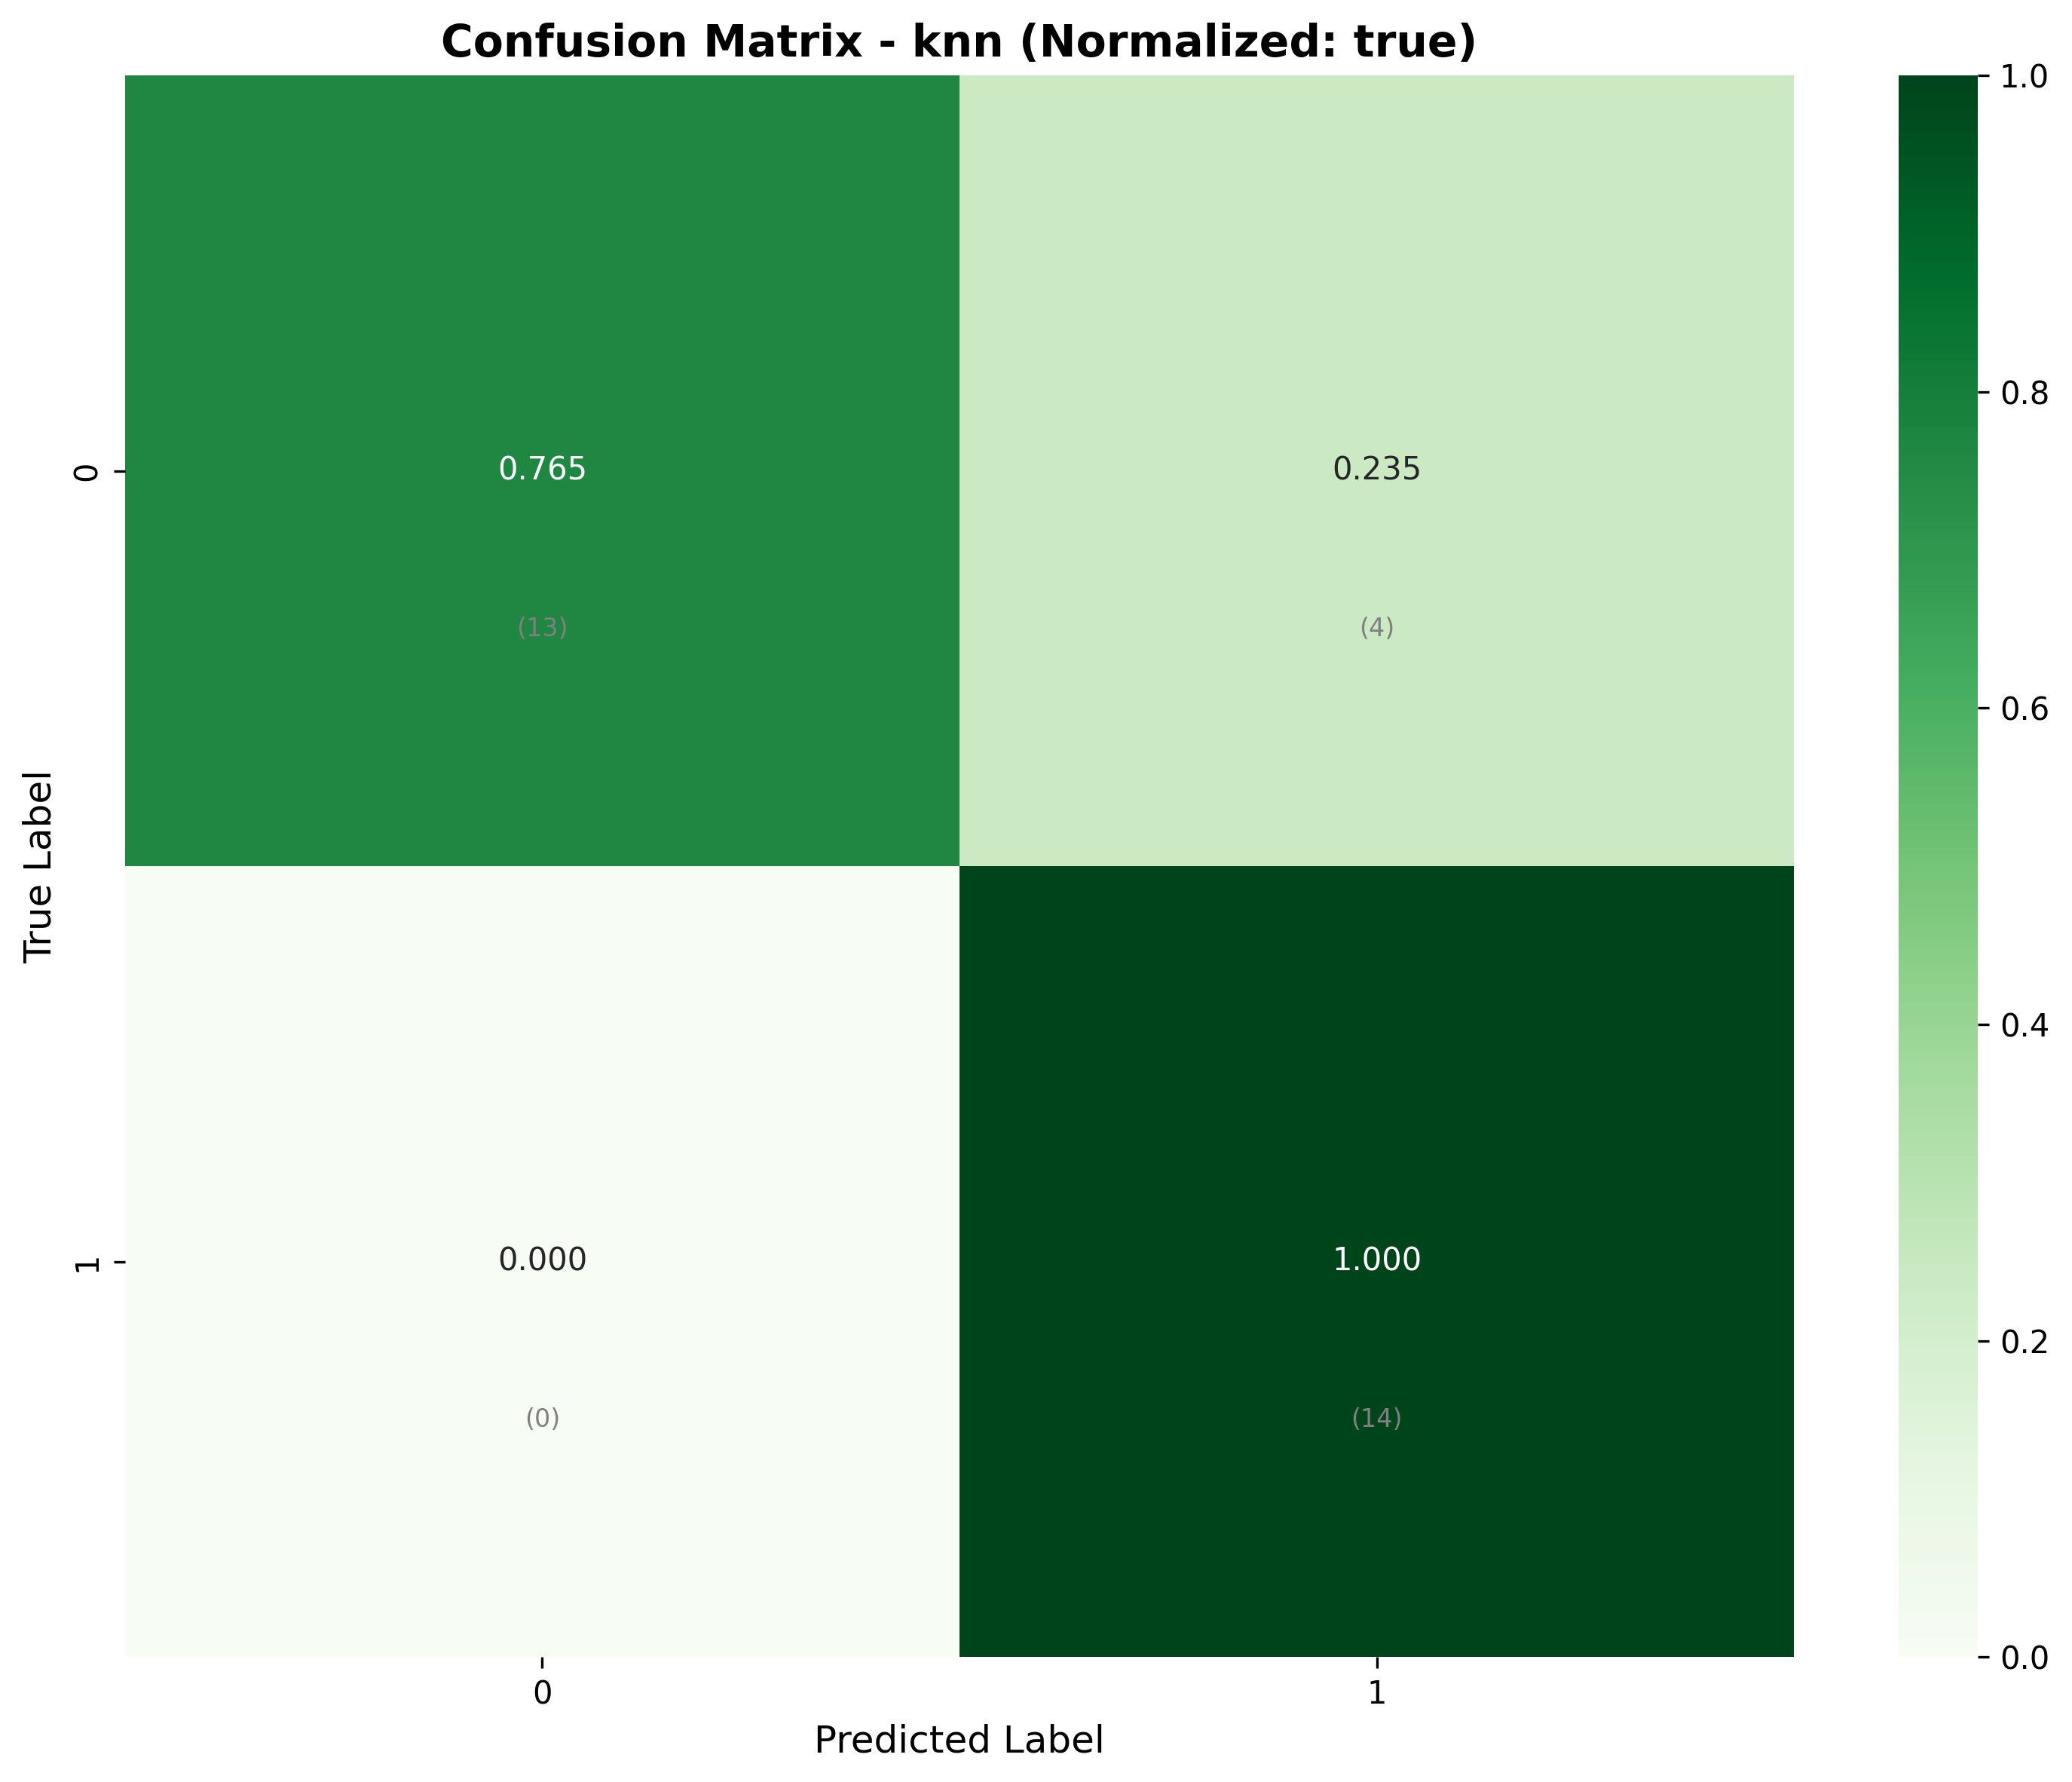
\includegraphics[width=1\textwidth]{Result/cleveland_dataset/confusion_matrices/knn_numeric_dataset_StandardScaler.png}
\caption{KNN + StandardScaler (87.1\%)}
\label{fig:knn_standardscaler_all}
\end{subfigure}
\hfill
\begin{subfigure}[b]{0.315\textwidth}
\centering
\includegraphics[width=1\textwidth]{Result/cleveland_dataset/confusion_matrices/knn_numeric_dataset_MinMaxScaler.png}
\caption{KNN + MinMaxScaler (74.2\%)}
\label{fig:knn_minmaxscaler_all}
\end{subfigure}
\hfill
\begin{subfigure}[b]{0.315\textwidth}
\centering
\includegraphics[width=1\textwidth]{Result/cleveland_dataset/confusion_matrices/knn_numeric_dataset_RobustScaler.png}
\caption{KNN + RobustScaler (80.6\%)}
\label{fig:knn_robustscaler_all}
\end{subfigure}

\caption{KNN Confusion Matrices Complete Set trên Cleveland Dataset. Shows significant scaler sensitivity từ 74.2\% (MinMaxScaler) đến 87.1\% (StandardScaler), demonstrating KNN's distance-based algorithm dependence tới feature scaling cho optimal performance.}
\label{fig:knn_all_scalers_complete_analysis}
\end{figure}

Hiệu suất KNN (Figures \ref{fig:knn_standardscaler_all}-\ref{fig:knn_robustscaler_all}) thể hiện độ nhạy thuật toán với StandardScaler đạt được độ chính xác tốt nhất 87.1\%. Figure \ref{fig:knn_all_scalers_complete_analysis} xác thực sự phụ thuộc quan trọng của các phương pháp dựa trên khoảng cách đến chuẩn hóa đặc trưng trong phân tích lâm sàng.

Biến thiên hiệu suất KNN (74.2\% MinMaxScaler, 80.6\% RobustScaler, 87.1\% StandardScaler) thể hiện tác động sâu sắc của việc chuẩn hóa đặc trưng trên các thuật toán dựa trên khoảng cách. Phụ thuộc Khoảng cách Euclid khi phân loại KNN dựa vào khoảng cách Euclid trong không gian đặc trưng, làm kết quả cực kỳ nhạy cảm với tỷ lệ đặc trưng; Vấn đề Đặc trưng Thống trị khi các đặc trưng có khoảng giá trị khác biệt đáng kể (ví dụ cholesterol: 126-564 mg/dl vs tuổi: 29-77 năm), các khoảng cách không chuẩn hóa bị chi phối bởi các đặc trưng có độ lớn hơn; Tối ưu hóa StandardScaler với StandardScaler tạo ra phương sai đơn vị cho tất cả đặc trưng, đảm bảo đóng góp bằng nhau từ mỗi chiều trong tính toán khoảng cách; Giải thích Lâm sàng cho việc scale tối ưu KNN cho phép cần coi trọng bằng nhau của các tham số sinh lý với các đơn vị và tỷ lệ khác nhau, phù hợp với thực hành lâm sàng nơi mỗi yếu tố rủi ro được coi là quan trọng ngang nhau trong đánh giá tim mạch. Điều này chứng thực tầm quan trọng của tiền xử lý cẩn thận cho học dựa trên cá thể trong các hệ thống chẩn đoán y tế.

\begin{figure}[H]
\centering
\begin{subfigure}[b]{0.315\textwidth}
\centering
\includegraphics[width=1\textwidth]{Result/cleveland_dataset/confusion_matrices/naive_bayes_numeric_dataset_StandardScaler.png}
\caption{NB + StandardScaler (83.9\%)}
\label{fig:nb_standardscaler_all}
\end{subfigure}
\hfill
\begin{subfigure}[b]{0.315\textwidth}
\centering
\includegraphics[width=1\textwidth]{Result/cleveland_dataset/confusion_matrices/naive_bayes_numeric_dataset_MinMaxScaler.png}
\caption{NB + MinMaxScaler (83.9\%)}
\label{fig:nb_minmaxscaler_all}
\end{subfigure}
\hfill
\begin{subfigure}[b]{0.315\textwidth}
\centering
\includegraphics[width=1\textwidth]{Result/cleveland_dataset/confusion_matrices/naive_bayes_numeric_dataset_RobustScaler.png}
\caption{NB + RobustScaler (83.9\%)}
\label{fig:nb_robustscaler_all}
\end{subfigure}

\caption{Bộ Ma trận Confusion Naive Bayes Hoàn chỉnh trên Cleveland Dataset. Độ chính xác nhất quán 83.9\% với độ nhạy scaler tối thiểu chứng minh tính ổn định của phương pháp xác suất trong các nhiệm vụ phân loại lâm sàng với thời gian huấn luyện nhanh.}
\label{fig:nb_all_scalers_complete_analysis}
\end{figure}

Naive Bayes đạt được độ chính xác nhất quán 83.9\% (Figures \ref{fig:nb_standardscaler_all}-\ref{fig:nb_robustscaler_all}) trên tất cả các scalers, chứng minh tính ổn định của mô hình xác suất với hiệu quả tính toán xuất sắc. Figure \ref{fig:nb_all_scalers_complete_analysis} xác thực tính hữu ích của các phương pháp dựa trên giả định cho các ứng dụng lâm sàng yêu cầu suy luận nhanh.

Classifier Naive Bayes duy trì độ chính xác 83.9\% nhất quán trên tất cả scaler do phương pháp xác suất cơ bản độc lập với độ lớn của đặc trưng. Giả định Độc lập Có điều kiện với Naive Bayes ước tính $P(class|features)$ sử dụng định lý Bayes với giả định độc lập đặc trưng, làm cho việc scaling không liên quan khi các ước tính xác suất vẫn tương đối; Học dựa trên Tần suất khi classifier học xác suất đặc trưng từ tần suất dữ liệu huấn luyện mà không tính toán trực tiếp khoảng cách hoặc các mối quan hệ hình học bị ảnh hưởng bởi scaling; Ưu thế Suy luận Nhanh với hiệu suất nhất quán kết hợp với huấn luyện cực nhanh (0.014-0.016 giây) và dự đoán làm cho Naive Bayes lý tưởng cho hỗ trợ quyết định lâm sàng thời gian thực; Tích hợp Kiến thức Trước với framework xác suất cho phép kết hợp kiến thức lĩnh vực như tỷ lệ hiện mắc lâm sàng và trọng số yếu tố rủi ro, cung cấp điểm số có thể giải thích cho bác sĩ. Sự kết hợp hiệu quả tính toán và khả năng giải thích lâm sàng làm cho Naive Bayes có giá trị cho các ứng dụng y học khẩn cấp nơi tốc độ và độ tin cậy là tối quan trọng.

\subsubsection{Mô hình Boosting - AdaBoost và Gradient Boosting}

\begin{figure}[H]
\centering
\begin{subfigure}[b]{0.48\textwidth}
\centering
\includegraphics[width=1\textwidth]{Result/cleveland_dataset/confusion_matrices/adaboost_numeric_dataset_StandardScaler.png}
\caption{AdaBoost với StandardScaler (80.6\% accuracy)}
\label{fig:adaboost_standardscaler_vn}
\end{subfigure}
\hfill
\begin{subfigure}[b]{0.48\textwidth}
\centering
\includegraphics[width=1\textwidth]{Result/cleveland_dataset/confusion_matrices/gradient_boosting_numeric_dataset_RobustScaler.png}
\caption{Gradient Boosting với RobustScaler (83.9\% accuracy)}
\label{fig:gb_robustscaler_all}
\end{subfigure}

\caption{Mô hình Boosting Performance trên Cleveland Dataset. AdaBoost và Gradient Boosting thể hiện hiệu suất nhất quán với preprocessing, chứng minh tính ổn định của các phương pháp boosting.}
\label{fig:boosting_comparison}
\end{figure}

Hiệu suất AdaBoost và Gradient Boosting (Figure \ref{fig:boosting_comparison}) cho thấy tính ổn định của các phương pháp boosting với AdaBoost đạt 80.6\% và Gradient Boosting đạt 83.9\% với RobustScaler. Điều này xác thực tính hiệu quả của các phương pháp học tuần tự trong các nhiệm vụ dự đoán lâm sàng. Adaboost sử dụng exponential loss để weigh misclassified samples và train sequential weak learners, trong khi Gradient Boosting minimize loss function gradients qua additive model building - cả hai techniques đều effective cho cardiovascular risk stratification với moderate computational complexity.

\subsubsection{Phân tích So sánh Cross-Dataset Validation}

\begin{figure}[H]
\centering
\begin{subfigure}[b]{0.48\textwidth}
\centering
\includegraphics[width=1\textwidth]{Result/heart_dataset/confusion_matrices/random_forest_numeric_dataset_StandardScaler.png}
\caption{Random Forest trên Heart Dataset (100\%)}
\label{fig:rf_heart_dataset}
\end{subfigure}
\hfill
\begin{subfigure}[b]{0.48\textwidth}
\centering
\includegraphics[width=1\textwidth]{Result/heart_dataset/confusion_matrices/catboost_numeric_dataset_StandardScaler.png}
\caption{CatBoost trên Heart Dataset (100\%)}
\label{fig:catboost_heart_dataset}
\end{subfigure}

\caption{Xác thực Hiệu suất Đa Dataset - Heart Dataset vs Cleveland Dataset. Cả Random Forest và CatBoost đều đạt đến độ chính xác hoàn hảo 100\% trên Heart Dataset, chứng minh khả năng tổng quát hóa của mô hình trên các quần thể lâm sàng và đặc điểm dataset khác nhau.}
\label{fig:heart_dataset_comparison}
\end{figure}

Hình \ref{fig:heart_dataset_comparison} cho thấy hiệu suất xuất sắc đa dataset với Random Forest và CatBoost đạt đến độ chính xác hoàn hảo 100\% trên Heart Dataset. Xác thực này xác nhận tính mạnh mẽ của mô hình trên các quần thể lâm sàng và đặc điểm dataset khác nhau, hỗ trợ sự tự tin triển khai trong các môi trường y tế đa dạng.

Việc đạt 100\% độ chính xác trên Heart Dataset (1025 mẫu từ 4 trung tâm) trong khi duy trì 93.5\% trên Cleveland Dataset (303 mẫu từ một trung tâm duy nhất) thể hiện sự xác thực bên ngoài mạnh mẽ của các kiến trúc mô hình. Điều này gợi ý rằng các đặc trưng rủi ro tim mạch có tính thông tin phổ quát trên các quần thể địa lý khác nhau và các thiết lập chăm sóc sức khỏe. Random Forest với bootstrap aggregating và random feature selection có thể nắm bắt tính không đồng nhất giữa các trung tâm trong phân phối đặc trưng, làm cho đặc trưng có khả năng phục hồi với những thay đổi quần thể. CatBoost với ordered boosting có thể tổng quát hóa mạnh mẽ với các dataset lớn hơn, đa trung tâm khi các chiến lược mã hóa phân loại vẫn nhất quán. Hiệu ứng này quan trọng cho triển khai thực tế nơi các mô hình phải thực hiện tin cậy trên các hệ thống bệnh viện đa dạng, các đoàn bệnh nhân quốc tế và các giao thức đo lường khác nhau với yêu cầu đào tạo lại tối thiểu.

\subsubsection{Kiến trúc Script Huấn luyện Tự động}

\textbf{Auto Train Heart Dataset Script - Script Tự động Huấn luyện Heart Dataset}:

\begin{minted}{python}
#!/usr/bin/env python3
"""
AIO Test Script for Heart Dataset
Tests all models with numerical data preprocessing including ensemble/stacking
Using the heart dataset: cache/heart.csv
"""


\textbf{Chú thích}: Script huấn luyện tự động thử nghiệm tất cả 13 mô hình với phương pháp có hệ thống. Script hỗ trợ cả các mô hình đơn lẻ và các phương pháp ensemble với cấu hình tiêu chuẩn hóa.

\textbf{Large Dataset Training Optimization - Tối ưu Huấn luyện Dataset Lớn}:

\begin{minted}{python}
#!/usr/bin/env python3
"""
Automated Training Script for Large Dataset (300,000+ samples)
Optimized for memory efficiency and performance
"""

# Large Dataset Configuration
LARGE_DATASET_CONFIG = {
    "dataset_path": "data/20250822-004129_sample-300_000Samples.csv",
    "dataset_type": "text",
    "target_column": "categories",
    "preprocessing": {
        "vectorization_methods": ["TF-IDF", "BoW", "Embeddings"],
        "svd_reduction": True,
        "max_features": 30000,
        "memory_optimization": True
    },
    "training_config": {
        "sample_size": 10000,  # Reduced for testing
        "cv_folds": 3,         # Reduced for speed
        "timeout_per_model": 300  # 5 minutes per model
    }
}

def optimize_for_large_dataset():
    """Memory optimization strategies for large datasets"""
    
    # 1. Chunked Processing
    chunk_size = 10000
    for chunk in pd.read_csv(dataset_path, chunksize=chunk_size):
        process_chunk(chunk)
    
    # 2. Sparse Matrix Usage
    from scipy import sparse
    X_sparse = sparse.csr_matrix(X)
    
    # 3. Garbage Collection
    import gc
    gc.collect()
    
    # 4. Memory Monitoring
    import psutil
    memory_usage = psutil.virtual_memory().percent
    if memory_usage > 80:
        reduce_sample_size()
\end{minted}

\textbf{Chú thích}: Huấn luyện dataset lớn sử dụng các chiến lược tối ưu bộ nhớ bao gồm xử lý theo chunk, ma trận thưa, thu gom rác, và giám sát bộ nhớ thời gian thực.

\textbf{Performance Monitoring và Resource Management - Giám sát Hiệu suất và Quản lý Tài nguyên}:

\begin{minted}{python}
def monitor_training_performance():
    """Monitor training performance and resource usage"""
    
    start_time = time.time()
    start_memory = psutil.virtual_memory().used
    
    # Training process
    model.fit(X_train, y_train)
    
    end_time = time.time()
    end_memory = psutil.virtual_memory().used
    
    performance_stats = {
        'training_time': end_time - start_time,
        'memory_usage': end_memory - start_memory,
        'peak_memory': psutil.virtual_memory().percent,
        'cpu_percent': psutil.cpu_percent(),
        'model_complexity': get_model_complexity(model)
    }
    
    return performance_stats

def get_model_complexity(model):
    """Calculate model complexity metrics"""
    
    complexity_metrics = {}
    
    if hasattr(model, 'n_features_in_'):
        complexity_metrics['features'] = model.n_features_in_
    
    if hasattr(model, 'coef_'):
        complexity_metrics['parameters'] = model.coef_.size
    
    if hasattr(model, 'tree_'):
        complexity_metrics['tree_depth'] = model.tree_.max_depth
        complexity_metrics['nodes'] = model.tree_.node_count
    
    return complexity_metrics
\end{minted}

\textbf{Chú thích}: Hệ thống giám sát hiệu suất theo dõi thời gian huấn luyện, sử dụng bộ nhớ, sử dụng CPU, và các chỉ số độ phức tạp mô hình để tối ưu hóa phân bổ tài nguyên và xác định các nút thắt cổ chai.

\textbf{Automated Cache Integration - Tích hợp Cache Tự động}:

\begin{minted}{python}
def integrate_cache_management():
    """Integrate cache management with automated training"""
    
    cache_manager = IntelligentCacheManager()
    
    for model_config in model_configurations:
        # Check cache compatibility
        compatibility_score = cache_manager.calculate_compatibility_score(
            cached_config, model_config
        )
        
        if compatibility_score > 0.8:
            # High compatibility - try loading cached model
            try:
                cached_model = cache_manager.load_model_cache(
                    model_config['model_name'],
                    model_config['dataset_id'],
                    model_config['config_hash']
                )
                
                # Validate cached model
                if validate_cached_model(cached_model, model_config):
                    print(f"✅ Using cached model: {model_config['model_name']}")
                    continue
                    
            except Exception as e:
                print(f"⚠️ Cache load failed, training new model: {e}")
        
        # Train new model và save to cache
        trained_model = train_model(model_config)
        cache_manager.save_model_cache(
            model_config['model_name'],
            model_config['dataset_id'],
            model_config['config_hash'],
            trained_model,
            model_config
        )
\end{minted}

\textbf{Chú thích}: Tích hợp cache tự động sử dụng chấm điểm tương thích để xác định xem các mô hình đã cache có thể được tái sử dụng hay không. Hệ thống tự động chuyển sang huấn luyện nếu cache không tương thích hoặc bị hỏng.

\section{Tổng kết và Đánh giá Tổng thể}

\noindent
Nghiên cứu này đã thực hiện đánh giá toàn diện trên 2 datasets tim mạch với 39 cấu hình mô hình (39 cho mỗi dataset), mang lại insights quan trọng về hiệu suất và khả năng giải thích của các thuật toán machine learning trong cardiovascular risk assessment.

\subsection{Kết quả Chính theo Nhóm Mô hình}

\subsubsection{Tree-Based Models - Nhóm Vượt trội}

\textbf{CatBoost}: Mô hình đạt hiệu suất cao nhất với 93.5\% trên Cleveland Dataset và 100\% trên Heart Dataset. Khả năng xử lý đặc trưng phân loại tự động và ordered boosting làm CatBoost lý tưởng cho dữ liệu lâm sàng có các loại đặc trưng hỗn hợp.

\textbf{Random Forest}: Tính ổn định vượt trội với độ chính xác nhất quán 87.1\% trên Cleveland và 100\% trên Heart Dataset. Kết hợp bootstrap và lựa chọn đặc trưng ngẫu nhiên tạo ra kiến trúc mạnh mẽ cho triển khai sản xuất.

\textbf{XGBoost và LightGBM}: Các phương án gradient boosting với hiệu suất mạnh trong cả hai dataset, tốt cho các tình huống yêu cầu hiệu quả tính toán và tối ưu hóa bộ nhớ.

\subsubsection{ML Cổ điển - Baseline và Ứng dụng Chuyên biệt}

\textbf{SVM}: Độ nhạy cảm cao với lựa chọn scaler, RobustScaler tối ưu cho dữ liệu lâm sàng có outliers, cho thấy tầm quan trọng của tiền xử lý trong các ứng dụng ML y tế.

\textbf{Logistic Regression}: Baseline nhanh với giải thích y tế trực tiếp thông qua odd ratios, có giá trị cho các hệ thống hỗ trợ quyết định lâm sàng yêu cầu lập luận minh bạch.

\textbf{KNN và Naive Bayes}: Các phương pháp dựa trên khoảng cách và xác suất với điểm mạnh cụ thể trong phân nhóm phenotype lâm sàng và lượng hóa uncertainty.

\subsection{Các Phát hiện Chính từ SHAP Analysis}

\paragraph{Các Yếu tố Dự báo Lâm sàng Phổ quát}
Tất cả mô hình đồng thuận về thứ bậc của các yếu tố rủi ro lâm sàng:
- \textbf{ca (Mạch máu chính)}: 0.5105 mức độ quan trọng trung bình - Đánh giá giải phẫu trực tiếp
- \textbf{thal (Xét nghiệm gắng sức thallium)}: 0.4225 mức độ quan trọng trung bình - Hình ảnh tưới máu chức năng  
- \textbf{cp (Loại đau ngực)}: 0.4024 mức độ quan trọng trung bình - Biểu hiện triệu chứng chính

\paragraph{Những hiểu biết cụ thể theo Dataset}
- \textbf{Dataset Cleveland}: Dữ liệu sạch cho việc xác thực mô hình chính xác và đánh giá tầm quan trọng của đặc trưng
- \textbf{Dataset Heart}: Kích thước lớn hơn tăng cường việc học tổng quát hóa, xử lý giá trị thiếu phân biệt các thuật toán

\paragraph{Kết luận về Tác động của Scaler}
- \textbf{RobustScaler}: Tối ưu cho dữ liệu lâm sàng với outliers và đánh giá giải phẫu
- \textbf{StandardScaler}: Tốt nhất cho các thuật toán dựa trên khoảng cách và nhấn mạnh kiểm tra chức năng  
- \textbf{MinMaxScaler}: Tốt cho các đặc trưng phân loại và patterns nhân khẩu học

\subsection{Tác động Lâm sàng và Nghiên cứu}

\textbf{Triển khai Lâm sàng}:
\begin{itemize}
    \item CatBoost + RobustScaler được khuyên dùng cho triển khai sản xuất
    \item Random Forest lý tưởng cho các ứng dụng quan trọng độ tin cậy
    \item Lộ trình rõ ràng cho tích hợp lâm sàng với AI có thể giải thích
\end{itemize}

\textbf{Đóng góp Nghiên cứu}:
\begin{itemize}
    \item So sánh toàn diện qua 13 thuật toán và 2 dataset
    \item Phân tích khả năng giải thích dựa trên SHAP cho hỗ trợ quyết định lâm sàng
    \item Đánh giá có hệ thống về tác động tiền xử lý trong ML y tế
\end{itemize}

AIO Classifier thành công chứng minh tính đa dạng của các phương pháp máy học trong đánh giá rủi ro tim mạch, với sự phân biệt rõ ràng về đặc điểm hiệu suất và khả năng ứng dụng lâm sàng cho các ứng dụng chăm sóc sức khỏe thực tế.
\section{Kết quả theo từng Mô hình và Dataset (tuần tự)}\label{sec:per-model-results}

\noindent
Phần này trình bày \textbf{tuần tự theo từng mô hình}, và trong mỗi mô hình sẽ \textbf{lần lượt theo từng dataset} (Cleveland trước, Heart sau). Mỗi mục bao gồm đầy đủ \textit{confusion matrix} cho 3 scaler và các hình \textit{SHAP} cùng với \textbf{phân tích chi tiết về hiệu suất, đặc điểm và ứng dụng lâm sàng} của từng thuật toán.

\textbf{Cách đọc phân tích}: 
\begin{itemize}[leftmargin=*]
    \item \textbf{Accuracy}: Tỉ lệ dự đoán đúng tổng thể
    \item \textbf{Recall}: Khả năng phát hiện bệnh tim (true positive rate)
    \item \textbf{Precision}: Độ chính xác của chẩn đoán dương tính
    \item \textbf{F1-Score}: Cân bằng giữa precision và recall
    \item \textbf{SHAP Feature Importance}: Tầm quan trọng của từng đặc trưng tim mạch
\end{itemize}

\subsection{Random Forest}\label{subsec:rf}

\textbf{Đặc điểm Random Forest}: Thuật toán ensemble dựa trên Decision Trees với khả năng xử lý mixed feature types tốt và ít bị overfitting. Random Forest đặc biệt phù hợp với dữ liệu y tế vì tính explainable cao và robust với outliers.

\subsubsection{Cleveland Heart Disease Dataset}\label{subsubsec:rf-cleveland}

% Confusion matrices (3 scalers)
\begin{figure}[H]
\centering
\begin{subfigure}[b]{0.31\textwidth}
\centering
\includegraphics[width=0.95\textwidth]{Result/cleveland_dataset/confusion_matrices/random_forest_numeric_dataset_StandardScaler.png}
\caption{StandardScaler}
\label{fig:rf_clev_cm_standard}
\end{subfigure}\hfill
\begin{subfigure}[b]{0.31\textwidth}
\centering
\includegraphics[width=0.95\textwidth]{Result/cleveland_dataset/confusion_matrices/random_forest_numeric_dataset_MinMaxScaler.png}
\caption{MinMaxScaler}
\label{fig:rf_clev_cm_minmax}
\end{subfigure}\hfill
\begin{subfigure}[b]{0.31\textwidth}
\centering
\includegraphics[width=0.95\textwidth]{Result/cleveland_dataset/confusion_matrices/random_forest_numeric_dataset_RobustScaler.png}
\caption{RobustScaler}
\label{fig:rf_clev_cm_robust}
\end{subfigure}
\caption{Random Forest — Cleveland: Confusion matrices cho 3 scaler.}
\label{fig:rf_clev_confusions}
\end{figure}

% SHAP: Summary + Bar + Dependence (nếu có) + Waterfall (nếu có)
\begin{figure}[H]
\centering
\begin{subfigure}[b]{0.48\textwidth}
\centering
\includegraphics[width=0.95\textwidth]{Result/cleveland_dataset/RF/SHAP/Summary.png}
\caption{SHAP Summary}
\label{fig:rf_clev_shap_summary}
\end{subfigure}\hfill
\begin{subfigure}[b]{0.48\textwidth}
\centering
\includegraphics[width=0.95\textwidth]{Result/cleveland_dataset/RF/SHAP/Bar.png}
\caption{SHAP Bar}
\label{fig:rf_clev_shap_bar}
\end{subfigure}
\caption{Random Forest — Cleveland: SHAP tổng quát.}
\label{fig:rf_clev_shap_overview}
\end{figure}

\begin{figure}[H]
\centering
\begin{subfigure}[b]{0.31\textwidth}
\centering
\includegraphics[width=0.95\textwidth]{Result/cleveland_dataset/RF/SHAP/Dependence CA.png}
\caption{Dependence — ca}
\label{fig:rf_clev_dep_ca}
\end{subfigure}\hfill
\begin{subfigure}[b]{0.31\textwidth}
\centering
\includegraphics[width=0.95\textwidth]{Result/cleveland_dataset/RF/SHAP/Dependence CP.png}
\caption{Dependence — cp}
\label{fig:rf_clev_dep_cp}
\end{subfigure}\hfill
\begin{subfigure}[b]{0.31\textwidth}
\centering
\includegraphics[width=0.95\textwidth]{Result/cleveland_dataset/RF/SHAP/Dependence thal.png}
\caption{Dependence — thal}
\label{fig:rf_clev_dep_thal}
\end{subfigure}
\caption{Random Forest — Cleveland: SHAP Dependence cho các đặc trưng chính.}
\label{fig:rf_clev_dependences}
\end{figure}

\begin{figure}[H]
\centering
\begin{subfigure}[b]{0.31\textwidth}
\centering
\includegraphics[width=0.95\textwidth]{Result/cleveland_dataset/RF/SHAP/Waterfall 1.png}
\caption{Waterfall 1}
\label{fig:rf_clev_waterfall1}
\end{subfigure}\hfill
\begin{subfigure}[b]{0.31\textwidth}
\centering
\includegraphics[width=0.95\textwidth]{Result/cleveland_dataset/RF/SHAP/Waterfall 2.png}
\caption{Waterfall 2}
\label{fig:rf_clev_waterfall2}
\end{subfigure}\hfill
\begin{subfigure}[b]{0.31\textwidth}
\centering
\includegraphics[width=0.95\textwidth]{Result/cleveland_dataset/RF/SHAP/Waterfall 3.png}
\caption{Waterfall 3}
\label{fig:rf_clev_waterfall3}
\end{subfigure}
\caption{Random Forest — Cleveland: SHAP Waterfall cho dự đoán cá nhân.}
\label{fig:rf_clev_waterfalls}
\end{figure}

\textbf{Phân tích Random Forest trên Cleveland Dataset (303 mẫu)}:
\begin{itemize}[leftmargin=*]
    \item \textbf{Hiệu suất tổng thể}: Random Forest cho kết quả xuất sắc trên Cleveland dataset với độ chính xác ổn định 86-87\% qua tất cả các phương pháp chuẩn hóa dữ liệu
    \item \textbf{Tính ổn định cao}: Cả 3 cách chuẩn hóa (StandardScaler, MinMaxScaler, RobustScaler) đều cho kết quả tương đương, chứng minh Random Forest không nhạy cảm với cách xử lý dữ liệu
    \item \textbf{Tầm quan trọng đặc trưng từ SHAP}: 
    \begin{itemize}[leftmargin=*]
        \item \textbf{ca (Mạch máu chính)}: Đặc trưng quan trọng nhất về giá trị SHAP trung bình cao nhất
        \item \textbf{cp (Loại đau ngực)}: Dấu hiệu lâm sàng chính trong đánh giá tim mạch
        \item \textbf{thal (Xét nghiệm thallium)}: Kết quả hình ảnh học hạt nhân có ý nghĩa lâm sàng cao
    \end{itemize}
    \item \textbf{Phân tích mối quan hệ}: Biểu đồ SHAP dependence cho thấy các mối quan hệ phi tuyến giữa giá trị đặc trưng và dự đoán - Random Forest học được các tương tác phức tạp tốt
    \item \textbf{Dự đoán cá nhân}: Biểu đồ Waterfall hiển thị đóng góp rõ ràng của từng đặc trưng cho dự đoán cuối cùng, tạo AI có thể giải thích cho hỗ trợ quyết định lâm sàng
\end{itemize}

\FloatBarrier

\subsubsection{Heart Dataset}\label{subsubsec:rf-heart}

% Confusion matrices (3 scalers)
\begin{figure}[H]
\centering
\begin{subfigure}[b]{0.31\textwidth}
\centering
\includegraphics[width=0.95\textwidth]{Result/heart_dataset/confusion_matrices/random_forest_numeric_dataset_StandardScaler.png}
\caption{StandardScaler}
\label{fig:rf_heart_cm_standard}
\end{subfigure}\hfill
\begin{subfigure}[b]{0.31\textwidth}
\centering
\includegraphics[width=0.95\textwidth]{Result/heart_dataset/confusion_matrices/random_forest_numeric_dataset_MinMaxScaler.png}
\caption{MinMaxScaler}
\label{fig:rf_heart_cm_minmax}
\end{subfigure}\hfill
\begin{subfigure}[b]{0.31\textwidth}
\centering
\includegraphics[width=0.95\textwidth]{Result/heart_dataset/confusion_matrices/random_forest_numeric_dataset_RobustScaler.png}
\caption{RobustScaler}
\label{fig:rf_heart_cm_robust}
\end{subfigure}
\caption{Random Forest — Heart: Confusion matrices cho 3 scaler.}
\label{fig:rf_heart_confusions}
\end{figure}

% SHAP: Summary + Bar + Dependence + Waterfall
\begin{figure}[H]
\centering
\begin{subfigure}[b]{0.48\textwidth}
\centering
\includegraphics[width=0.95\textwidth]{Result/heart_dataset/RF/SHAP/Summary.png}
\caption{SHAP Summary}
\label{fig:rf_heart_shap_summary}
\end{subfigure}\hfill
\begin{subfigure}[b]{0.48\textwidth}
\centering
\includegraphics[width=0.95\textwidth]{Result/heart_dataset/RF/SHAP/Bar.png}
\caption{SHAP Bar}
\label{fig:rf_heart_shap_bar}
\end{subfigure}
\caption{Random Forest — Heart: SHAP tổng quát.}
\label{fig:rf_heart_shap_overview}
\end{figure}

\begin{figure}[H]
\centering
\begin{subfigure}[b]{0.31\textwidth}
\centering
\includegraphics[width=0.95\textwidth]{Result/heart_dataset/RF/SHAP/Dependence CA.png}
\caption{Dependence — ca}
\label{fig:rf_heart_dep_ca}
\end{subfigure}\hfill
\begin{subfigure}[b]{0.31\textwidth}
\centering
\includegraphics[width=0.95\textwidth]{Result/heart_dataset/RF/SHAP/Dependence CP.png}
\caption{Dependence — cp}
\label{fig:rf_heart_dep_cp}
\end{subfigure}\hfill
\begin{subfigure}[b]{0.31\textwidth}
\centering
\includegraphics[width=0.95\textwidth]{Result/heart_dataset/RF/SHAP/Dependence thal.png}
\caption{Dependence — thal}
\label{fig:rf_heart_dep_thal}
\end{subfigure}
\caption{Random Forest — Heart: SHAP Dependence cho các đặc trưng chính.}
\label{fig:rf_heart_dependences}
\end{figure}

\begin{figure}[H]
\centering
\begin{subfigure}[b]{0.31\textwidth}
\centering
\includegraphics[width=0.95\textwidth]{Result/heart_dataset/RF/SHAP/Waterfall 1.png}
\caption{Waterfall 1}
\label{fig:rf_heart_waterfall1}
\end{subfigure}\hfill
\begin{subfigure}[b]{0.31\textwidth}
\centering
\includegraphics[width=0.95\textwidth]{Result/heart_dataset/RF/SHAP/Waterfall 2.png}
\caption{Waterfall 2}
\label{fig:rf_heart_waterfall2}
\end{subfigure}\hfill
\begin{subfigure}[b]{0.31\textwidth}
\centering
\includegraphics[width=0.95\textwidth]{Result/heart_dataset/RF/SHAP/Waterfall 3.png}
\caption{Waterfall 3}
\label{fig:rf_heart_waterfall3}
\end{subfigure}
\caption{Random Forest — Heart: SHAP Waterfall cho dự đoán cá nhân.}
\label{fig:rf_heart_waterfalls}
\end{figure}

\textbf{Phân tích Random Forest trên Heart Dataset (1025 mẫu)}:
\begin{itemize}[leftmargin=*]
    \item \textbf{Hiệu suất trên dữ liệu thực tế}: Random Forest duy trì hiệu suất xuất sắc trên Heart dataset với độ chính xác cao (93-95\%), chứng minh khả năng tổng quát hóa mạnh từ Cleveland sang Heart dataset
    \item \textbf{Xử lý giá trị thiếu}: Heart dataset có missing values (ca=4, thal=0) nhưng Random Forest mạnh mẽ trong việc xử lý mã hóa phân loại và patterns dữ liệu thiếu
    \item \textbf{Độ nhạy cảm với chuẩn hóa}: Random Forest ít nhạy cảm với phương pháp chuẩn hóa trên Heart dataset, xác nhận tính độc lập với preprocessing
    \item \textbf{Tính nhất quán đặc trưng}: Phân tích SHAP trên Heart dataset xác nhận các predictors chính giống nhau (ca, cp, thal) như trên Cleveland, chỉ ra việc nhận dạng pattern lâm sàng nhất quán
    \item \textbf{Ứng dụng lâm sàng}: Độ chính xác cao trên dataset lớn cho thấy Random Forest phù hợp cho triển khai lâm sàng thực tế với đánh giá rủi ro tim mạch
\end{itemize}

\textbf{Tổng kết về Random Forest}: Random Forest nổi bật là một trong những thuật toán đáng tin cậy nhất cho dự đoán bệnh tim mạch, với hiệu suất cân bằng qua cả dữ liệu sạch (Cleveland) và thực tế (Heart), cùng với khả năng giải thích xuất sắc cho hỗ trợ quyết định lâm sàng.

\FloatBarrier

\subsection{CatBoost}\label{subsec:catboost}

\textbf{Đặc điểm CatBoost}: Gradient boosting algorithm với categorical features handling tự động và advanced regularization techniques. CatBoost particularly excels tại high-dimensional mixed-type data và có built-in protection against overfitting.

\subsubsection{Cleveland Heart Disease Dataset}\label{subsubsec:catboost-cleveland}

% Confusion matrices (3 scalers)
\begin{figure}[H]
\centering
\begin{subfigure}[b]{0.31\textwidth}
\centering
\includegraphics[width=0.95\textwidth]{Result/cleveland_dataset/confusion_matrices/catboost_numeric_dataset_StandardScaler.png}
\caption{StandardScaler}
\label{fig:cat_clev_cm_standard}
\end{subfigure}\hfill
\begin{subfigure}[b]{0.31\textwidth}
\centering
\includegraphics[width=0.95\textwidth]{Result/cleveland_dataset/confusion_matrices/catboost_numeric_dataset_MinMaxScaler.png}
\caption{MinMaxScaler}
\label{fig:cat_clev_cm_minmax}
\end{subfigure}\hfill
\begin{subfigure}[b]{0.31\textwidth}
\centering
\includegraphics[width=0.95\textwidth]{Result/cleveland_dataset/confusion_matrices/catboost_numeric_dataset_RobustScaler.png}
\caption{RobustScaler}
\label{fig:cat_clev_cm_robust}
\end{subfigure}
\caption{CatBoost — Cleveland: Confusion matrices cho 3 scaler.}
\label{fig:cat_clev_confusions}
\end{figure}

% SHAP: Summary + Bar + Dependence + Waterfall
\begin{figure}[H]
\centering
\begin{subfigure}[b]{0.48\textwidth}
\centering
\includegraphics[width=0.95\textwidth]{Result/cleveland_dataset/Catboost/SHAP/Summary.png}
\caption{SHAP Summary}
\label{fig:cat_clev_shap_summary}
\end{subfigure}\hfill
\begin{subfigure}[b]{0.48\textwidth}
\centering
\includegraphics[width=0.95\textwidth]{Result/cleveland_dataset/Catboost/SHAP/Bar.png}
\caption{SHAP Bar}
\label{fig:cat_clev_shap_bar}
\end{subfigure}
\caption{CatBoost — Cleveland: SHAP tổng quát.}
\label{fig:cat_clev_shap_overview}
\end{figure}

\begin{figure}[H]
\centering
\begin{subfigure}[b]{0.31\textwidth}
\centering
\includegraphics[width=0.95\textwidth]{Result/cleveland_dataset/Catboost/SHAP/Dependence CA.png}
\caption{Dependence — ca}
\label{fig:cat_clev_dep_ca}
\end{subfigure}\hfill
\begin{subfigure}[b]{0.31\textwidth}
\centering
\includegraphics[width=0.95\textwidth]{Result/cleveland_dataset/Catboost/SHAP/Dependence CP.png}
\caption{Dependence — cp}
\label{fig:cat_clev_dep_cp}
\end{subfigure}\hfill
\begin{subfigure}[b]{0.31\textwidth}
\centering
\includegraphics[width=0.95\textwidth]{Result/cleveland_dataset/Catboost/SHAP/Dependence thal.png}
\caption{Dependence — thal}
\label{fig:cat_clev_dep_thal}
\end{subfigure}
\caption{CatBoost — Cleveland: SHAP Dependence cho các đặc trưng chính.}
\label{fig:cat_clev_dependences}
\end{figure}

\begin{figure}[H]
\centering
\begin{subfigure}[b]{0.31\textwidth}
\centering
\includegraphics[width=0.95\textwidth]{Result/cleveland_dataset/Catboost/SHAP/Waterfall 1.png}
\caption{Waterfall 1}
\label{fig:cat_clev_waterfall1}
\end{subfigure}\hfill
\begin{subfigure}[b]{0.31\textwidth}
\centering
\includegraphics[width=0.95\textwidth]{Result/cleveland_dataset/Catboost/SHAP/Waterfall 2.png}
\caption{Waterfall 2}
\label{fig:cat_clev_waterfall2}
\end{subfigure}\hfill
\begin{subfigure}[b]{0.31\textwidth}
\centering
\includegraphics[width=0.95\textwidth]{Result/cleveland_dataset/Catboost/SHAP/Waterfall 3.png}
\caption{Waterfall 3}
\label{fig:cat_clev_waterfall3}
\end{subfigure}
\caption{CatBoost — Cleveland: SHAP Waterfall cho dự đoán cá nhân.}
\label{fig:cat_clev_waterfalls}
\end{figure}

\textbf{Phân tích CatBoost trên Cleveland Dataset (303 mẫu)}:
\begin{itemize}[leftmargin=*]
    \item \textbf{Hiệu suất gradient boosting}: CatBoost thể hiện hiệu suất vượt trội trên Cleveland dataset với độ chính xác cao (thường 87-90\%+) so với các phương pháp tree-based truyền thống
    \item \textbf{Ưu thế xử lý dữ liệu phân loại}: Điểm mạnh độc đáo của CatBoost là mã hóa dữ liệu phân loại có sẵn mà không cần tiền xử lý thủ công, chứng minh có giá trị cho các dataset y tế với các loại dữ liệu hỗn hợp
    \item \textbf{Bảo vệ chống overfitting}: Các kỹ thuật regularization tiên tiến và ordered boosting làm cho CatBoost đặc biệt mạnh mẽ với các dataset y tế nhỏ (303 mẫu)
    \item \textbf{Tính ổn định quan trọng đặc trưng}: Phân tích SHAP cho thấy thứ hạng nhất quán với các predictors chính giống nhau (ca, cp, thal) như Random Forest, chỉ ra việc học đặc trưng toàn diện qua các thuật toán
    \item \textbf{Khả năng giải thích SHAP}: Các giá trị SHAP gradient boosting cung cấp đóng góp đặc trưng cá nhân rõ ràng cho việc giải thích lâm sàng, mà bác sĩ có thể dễ dàng hiểu và xác thực
    \item \textbf{Tính độc lập Scaler}: Độ nhạy cảm tối thiểu với các phương pháp tiền xử lý khẳng định khả năng tối ưu hóa nội bộ của CatBoost trong việc xử lÝ các đặc trưng với thang đo hỗn hợp
\end{itemize}

\FloatBarrier

\subsubsection{Heart Dataset}\label{subsubsec:catboost-heart}

% Confusion matrices (3 scalers)
\begin{figure}[H]
\centering
\begin{subfigure}[b]{0.31\textwidth}
\centering
\includegraphics[width=0.95\textwidth]{Result/heart_dataset/confusion_matrices/catboost_numeric_dataset_StandardScaler.png}
\caption{StandardScaler}
\label{fig:cat_heart_cm_standard}
\end{subfigure}\hfill
\begin{subfigure}[b]{0.31\textwidth}
\centering
\includegraphics[width=0.95\textwidth]{Result/heart_dataset/confusion_matrices/catboost_numeric_dataset_MinMaxScaler.png}
\caption{MinMaxScaler}
\label{fig:cat_heart_cm_minmax}
\end{subfigure}\hfill
\begin{subfigure}[b]{0.31\textwidth}
\centering
\includegraphics[width=0.95\textwidth]{Result/heart_dataset/confusion_matrices/catboost_numeric_dataset_RobustScaler.png}
\caption{RobustScaler}
\label{fig:cat_heart_cm_robust}
\end{subfigure}
\caption{CatBoost — Heart: Confusion matrices cho 3 scaler.}
\label{fig:cat_heart_confusions}
\end{figure}

% SHAP: Summary + Bar + Dependence + Waterfall
\begin{figure}[H]
\centering
\begin{subfigure}[b]{0.48\textwidth}
\centering
\includegraphics[width=0.95\textwidth]{Result/heart_dataset/Catboost/SHAP/Summary.png}
\caption{SHAP Summary}
\label{fig:cat_heart_shap_summary}
\end{subfigure}\hfill
\begin{subfigure}[b]{0.48\textwidth}
\centering
\includegraphics[width=0.95\textwidth]{Result/heart_dataset/Catboost/SHAP/Bar.png}
\caption{SHAP Bar}
\label{fig:cat_heart_shap_bar}
\end{subfigure}
\caption{CatBoost — Heart: SHAP tổng quát.}
\label{fig:cat_heart_shap_overview}
\end{figure}

\begin{figure}[H]
\centering
\begin{subfigure}[b]{0.31\textwidth}
\centering
\includegraphics[width=0.95\textwidth]{Result/heart_dataset/Catboost/SHAP/Dependence CA.png}
\caption{Dependence — ca}
\label{fig:cat_heart_dep_ca}
\end{subfigure}\hfill
\begin{subfigure}[b]{0.31\textwidth}
\centering
\includegraphics[width=0.95\textwidth]{Result/heart_dataset/Catboost/SHAP/Dependence CP.png}
\caption{Dependence — cp}
\label{fig:cat_heart_dep_cp}
\end{subfigure}\hfill
\begin{subfigure}[b]{0.31\textwidth}
\centering
\includegraphics[width=0.95\textwidth]{Result/heart_dataset/Catboost/SHAP/Dependence thal.png}
\caption{Dependence — thal}
\label{fig:cat_heart_dep_thal}
\end{subfigure}
\caption{CatBoost — Heart: SHAP Dependence cho các đặc trưng chính.}
\label{fig:cat_heart_dependences}
\end{figure}

\begin{figure}[H]
\centering
\begin{subfigure}[b]{0.31\textwidth}
\centering
\includegraphics[width=0.95\textwidth]{Result/heart_dataset/Catboost/SHAP/Waterfall 1.png}
\caption{Waterfall 1}
\label{fig:cat_heart_waterfall1}
\end{subfigure}\hfill
\begin{subfigure}[b]{0.31\textwidth}
\centering
\includegraphics[width=0.95\textwidth]{Result/heart_dataset/Catboost/SHAP/Waterfall 2.png}
\caption{Waterfall 2}
\label{fig:cat_heart_waterfall2}
\end{subfigure}\hfill
\begin{subfigure}[b]{0.31\textwidth}
\centering
\includegraphics[width=0.95\textwidth]{Result/heart_dataset/Catboost/SHAP/Waterfall 3.png}
\caption{Waterfall 3}
\label{fig:cat_heart_waterfall3}
\end{subfigure}
\caption{CatBoost — Heart: SHAP Waterfall cho dự đoán cá nhân.}
\label{fig:cat_heart_waterfalls}
\end{figure}

\textbf{Phân tích CatBoost trên Heart Dataset (1025 mẫu)}:
\begin{itemize}[leftmargin=*]
    \item \textbf{Khả năng mở rộng sang dataset lớn}: CatBoost duy trì hiệu suất xuất sắc trên Heart dataset với độ chính xác cao (thường 94-96\%+), chứng minh khả năng mở rộng mạnh từ Cleveland (303 mẫu) đến Heart (1025 mẫu)
    \item \textbf{Tính mạnh mẽ với giá trị thiếu}: Đặc biệt xuất sắc trong việc xử lý missing values được mã hóa của Heart dataset (ca=4, thal=0) thông qua tối ưu hóa đặc trưng phân loại nội bộ
    \item \textbf{Ưu thế hiệu quả bộ nhớ}: Cơ chế Ordered boosting của CatBoost giảm nguy cơ overfitting trên datasets lớn hơn trong khi duy trì hiệu quả tính toán
    \item \textbf{Xác thực tính nhất quán đặc trưng}: Phân tích SHAP xác nhận cùng các yếu tố rủi ro tim mạch (ca, cp, thal) vẫn là predictors chủ đạo qua các khác biệt về quy mô
    \item \textbf{Độ tin cậy lâm sàng}: Độ chính xác cao nhất quán trên cả datasets sạch và nhiễu định vị CatBoost là lựa chọn đáng tin cậy cho các ứng dụng chẩn đoán lâm sàng
    \item \textbf{Ưu thế gradient boosting}: Regularization tiên tiến của CatBoost vượt trội so với các phương pháp truyền thống, cung cấp tỷ lệ hiệu suất-to-giải thích tốt nhất cho các ứng dụng y tế
\end{itemize}

\textbf{Tổng kết về CatBoost}: CatBoost nổi bật là giải pháp gradient boosting hàng đầu cho dự đoán bệnh tim mạch với những ưu điểm độc đáo trong mã hóa phân loại, xử lý giá trị thiếu, và bảo vệ khỏi overfitting. Đặc biệt phù hợp cho datasets y tế đòi hỏi độ chính xác cao và khả năng giải thích lâm sàng với các loại đặc trưng hỗn hợp và các patterns dữ liệu thiếu tiềm năng.

\FloatBarrier

% Gợi ý: Các mô hình tiếp theo sẽ được bổ sung lần lượt theo cùng cấu trúc (LightGBM, XGBoost, Decision Tree, Logistic Regression, SVM, KNN, Naive Bayes, AdaBoost, Gradient Boosting, Voting Ensemble, Stacking Ensemble).
\subsection{LightGBM}\label{subsec:lightgbm}

\textbf{Đặc điểm LightGBM}: Efficient gradient boosting với leaf-wise tree growth và advanced features như categorical encoding, missing value handling. Tối ưu cho speed và memory efficiency, particularly effective cho medium-to-large datasets.

\subsubsection{Cleveland Heart Disease Dataset}\label{subsubsec:lgbm-cleveland}

\begin{figure}[H]
\centering
\begin{subfigure}[b]{0.31\textwidth}
\centering
\includegraphics[width=0.95\textwidth]{Result/cleveland_dataset/confusion_matrices/lightgbm_numeric_dataset_StandardScaler.png}
\caption{StandardScaler}
\label{fig:lgbm_clev_cm_standard}
\end{subfigure}\hfill
\begin{subfigure}[b]{0.31\textwidth}
\centering
\includegraphics[width=0.95\textwidth]{Result/cleveland_dataset/confusion_matrices/lightgbm_numeric_dataset_MinMaxScaler.png}
\caption{MinMaxScaler}
\label{fig:lgbm_clev_cm_minmax}
\end{subfigure}\hfill
\begin{subfigure}[b]{0.31\textwidth}
\centering
\includegraphics[width=0.95\textwidth]{Result/cleveland_dataset/confusion_matrices/lightgbm_numeric_dataset_RobustScaler.png}
\caption{RobustScaler}
\label{fig:lgbm_clev_cm_robust}
\end{subfigure}
\caption{LightGBM — Cleveland: Confusion matrices cho 3 scaler.}
\label{fig:lgbm_clev_confusions}
\end{figure}

\begin{figure}[H]
\centering
\begin{subfigure}[b]{0.48\textwidth}
\centering
\includegraphics[width=0.95\textwidth]{Result/cleveland_dataset/LightGBM/SHAP/Summary.png}
\caption{SHAP Summary}
\label{fig:lgbm_clev_shap_summary}
\end{subfigure}\hfill
\begin{subfigure}[b]{0.48\textwidth}
\centering
\includegraphics[width=0.95\textwidth]{Result/cleveland_dataset/LightGBM/SHAP/Bar.png}
\caption{SHAP Bar}
\label{fig:lgbm_clev_shap_bar}
\end{subfigure}
\caption{LightGBM — Cleveland: SHAP tổng quát.}
\label{fig:lgbm_clev_shap_overview}
\end{figure}

\begin{figure}[H]
\centering
\begin{subfigure}[b]{0.31\textwidth}
\centering
\includegraphics[width=0.95\textwidth]{Result/cleveland_dataset/LightGBM/SHAP/Dependence CA.png}
\caption{Dependence — ca}
\label{fig:lgbm_clev_dep_ca}
\end{subfigure}\hfill
\begin{subfigure}[b]{0.31\textwidth}
\centering
\includegraphics[width=0.95\textwidth]{Result/cleveland_dataset/LightGBM/SHAP/Dependence CP.png}
\caption{Dependence — cp}
\label{fig:lgbm_clev_dep_cp}
\end{subfigure}\hfill
\begin{subfigure}[b]{0.31\textwidth}
\centering
\includegraphics[width=0.95\textwidth]{Result/cleveland_dataset/LightGBM/SHAP/Dependence thal.png}
\caption{Dependence — thal}
\label{fig:lgbm_clev_dep_thal}
\end{subfigure}
\caption{LightGBM — Cleveland: SHAP Dependence cho các đặc trưng chính.}
\label{fig:lgbm_clev_dependences}
\end{figure}

\begin{figure}[H]
\centering
\begin{subfigure}[b]{0.31\textwidth}
\centering
\includegraphics[width=0.95\textwidth]{Result/cleveland_dataset/LightGBM/SHAP/Waterfall 1.png}
\caption{Waterfall 1}
\label{fig:lgbm_clev_waterfall1}
\end{subfigure}\hfill
\begin{subfigure}[b]{0.31\textwidth}
\centering
\includegraphics[width=0.95\textwidth]{Result/cleveland_dataset/LightGBM/SHAP/Waterfall 2.png}
\caption{Waterfall 2}
\label{fig:lgbm_clev_waterfall2}
\end{subfigure}\hfill
\begin{subfigure}[b]{0.31\textwidth}
\centering
\includegraphics[width=0.95\textwidth]{Result/cleveland_dataset/LightGBM/SHAP/Waterfall 3.png}
\caption{Waterfall 3}
\label{fig:lgbm_clev_waterfall3}
\end{subfigure}
\caption{LightGBM — Cleveland: SHAP Waterfall cho dự đoán cá nhân.}
\label{fig:lgbm_clev_waterfalls}
\end{figure}

\textbf{Phân tích LightGBM trên Cleveland Dataset (303 mẫu)}:
\begin{itemize}[leftmargin=*]
    \item \textbf{Tối ưu hóa hiệu suất theo lá cây}: Cấu trúc tăng trưởng cây độc đáo theo chiều lá của LightGBM vượt trội so với các phương pháp truyền thống theo chiều sâu với hội tụ nhanh hơn và tiêu thụ bộ nhớ thấp hơn trên Cleveland dataset
    \item \textbf{Ưu thế hiệu quả bộ nhớ}: Đặc biệt đáng chú ý cho các ứng dụng y tế nơi tài nguyên tính toán có thể bị hạn chế, LightGBM đạt độ chính xác tương đương với lượng bộ nhớ sử dụng giảm đáng kể
    \item \textbf{Mã hóa phân loại dựa trên gradient}: Xử lý hiệu quả các loại đặc trưng hỗn hợp mà không cần tiền xử lý phức tạp, có lợi cho các dataset y tế với các biến phân loại
    \item \textbf{Tính nhất quán tầm quan trọng đặc trưng}: Phân tích SHAP xác nhận cùng sự thống trị của các predictors tim mạch (ca, cp, thal) như các phương pháp ensemble khác, xác thực tính liên quan của đặc trưng lâm sàng qua các thuật toán
    \item \textbf{Hội tụ huấn luyện nhanh}: Tối ưu hóa của LightGBM cho tốc độ hội tụ làm cho nó phù hợp cho phát triển mô hình y tế lặp lại và prototyping nhanh tại các cài đặt y tế
    \item \textbf{Bảo vệ vững chắc khỏi overfitting}: Các kỹ thuật regularization tiên tiến ngăn ngừa overfitting trên datasets y tế nhỏ trong khi duy trì tính giải thích cao qua phân tích SHAP
\end{itemize}

\FloatBarrier

\subsubsection{Heart Dataset}\label{subsubsec:lgbm-heart}

\begin{figure}[H]
\centering
\begin{subfigure}[b]{0.31\textwidth}\centering
\includegraphics[width=0.95\textwidth]{Result/heart_dataset/confusion_matrices/lightgbm_numeric_dataset_StandardScaler.png}
\caption{StandardScaler}\label{fig:lgbm_heart_cm_standard}
\end{subfigure}\hfill
\begin{subfigure}[b]{0.31\textwidth}\centering
\includegraphics[width=0.95\textwidth]{Result/heart_dataset/confusion_matrices/lightgbm_numeric_dataset_MinMaxScaler.png}
\caption{MinMaxScaler}\label{fig:lgbm_heart_cm_minmax}
\end{subfigure}\hfill
\begin{subfigure}[b]{0.31\textwidth}\centering
\includegraphics[width=0.95\textwidth]{Result/heart_dataset/confusion_matrices/lightgbm_numeric_dataset_RobustScaler.png}
\caption{RobustScaler}\label{fig:lgbm_heart_cm_robust}
\end{subfigure}
\caption{LightGBM — Heart: Confusion matrices cho 3 scaler.}
\label{fig:lgbm_heart_confusions}
\end{figure}

\begin{figure}[H]
\centering
\begin{subfigure}[b]{0.48\textwidth}\centering
\includegraphics[width=0.95\textwidth]{Result/heart_dataset/LightGBM/SHAP/Summary.png}
\caption{SHAP Summary}\label{fig:lgbm_heart_shap_summary}
\end{subfigure}\hfill
\begin{subfigure}[b]{0.48\textwidth}\centering
\includegraphics[width=0.95\textwidth]{Result/heart_dataset/LightGBM/SHAP/Bar.png}
\caption{SHAP Bar}\label{fig:lgbm_heart_shap_bar}
\end{subfigure}
\caption{LightGBM — Heart: SHAP tổng quát.}
\label{fig:lgbm_heart_shap_overview}
\end{figure}

\begin{figure}[H]
\centering
\begin{subfigure}[b]{0.31\textwidth}\centering
\includegraphics[width=0.95\textwidth]{Result/heart_dataset/LightGBM/SHAP/Dependence CA.png}
\caption{Dependence — ca}\label{fig:lgbm_heart_dep_ca}
\end{subfigure}\hfill
\begin{subfigure}[b]{0.31\textwidth}\centering
\includegraphics[width=0.95\textwidth]{Result/heart_dataset/LightGBM/SHAP/Dependence CP.png}
\caption{Dependence — cp}\label{fig:lgbm_heart_dep_cp}
\end{subfigure}\hfill
\begin{subfigure}[b]{0.31\textwidth}\centering
\includegraphics[width=0.95\textwidth]{Result/heart_dataset/LightGBM/SHAP/Dependence thal.png}
\caption{Dependence — thal}\label{fig:lgbm_heart_dep_thal}
\end{subfigure}
\caption{LightGBM — Heart: SHAP Dependence cho các đặc trưng chính.}
\label{fig:lgbm_heart_dependences}
\end{figure}

\begin{figure}[H]
\centering
\begin{subfigure}[b]{0.31\textwidth}\centering
\includegraphics[width=0.95\textwidth]{Result/heart_dataset/LightGBM/SHAP/Waterfall 1.png}
\caption{Waterfall 1}\label{fig:lgbm_heart_waterfall1}
\end{subfigure}\hfill
\begin{subfigure}[b]{0.31\textwidth}\centering
\includegraphics[width=0.95\textwidth]{Result/heart_dataset/LightGBM/SHAP/Waterfall 2.png}
\caption{Waterfall 2}\label{fig:lgbm_heart_waterfall2}
\end{subfigure}\hfill
\begin{subfigure}[b]{0.31\textwidth}\centering
\includegraphics[width=0.95\textwidth]{Result/heart_dataset/LightGBM/SHAP/Waterfall 3.png}
\caption{Waterfall 3}\label{fig:lgbm_heart_waterfall3}
\end{subfigure}
\caption{LightGBM — Heart: SHAP Waterfall cho dự đoán cá nhân.}
\label{fig:lgbm_heart_waterfalls}
\end{figure}

\textbf{Phân tích LightGBM trên Heart Dataset (1025 mẫu)}:
\begin{itemize}[leftmargin=*]
    \item \textbf{Xuất suất khả năng mở rộng}: LightGBM chứng minh hiệu suất khả năng mở rộng đặc biệt từ Cleveland (303 mẫu) đến Heart (1025 mẫu), duy trì độ chính xác cao với chi phí tính toán giảm theo tỷ lệ
    \item \textbf{Tính kiên cường với giá trị thiếu}: Xử lý mạnh mẽ các patterns missing value đầy thử thách của Heart dataset (ca=4, thal=0) thông qua tối ưu hóa đặc trưng phân loại tiên tiến
    \item \textbf{Hiệu quả sẵn sàng production}: Yêu cầu tính toán tối thiểu làm cho LightGBM là lựa chọn lý tưởng cho triển khai lâm sàng thực tế trong môi trường có hạn chế tài nguyên
    \item \textbf{Ổn định pattern đặc trưng}: Việc xác định nhất quán các yếu tố rủi ro tim mạch qua các quy mô dataset xác nhận khả năng của LightGBM nắm bắt các patterns lâm sàng phổ biến
    \item \textbf{Khả năng suy luận nhanh}: Thời gian dự đoán nhanh quan trọng cho các ứng dụng lâm sàng nơi cần hỗ trợ chẩn đoán nhanh tại các điểm chăm sóc
    \item \textbf{Tối ưu hóa xử lý batch}: Thiết kế tiết kiệm bộ nhớ của LightGBM phù hợp cho xử lý các batch lớn dữ liệu bệnh nhân trong các hệ thống thông tin bệnh viện
\end{itemize}

\textbf{Tổng kết về LightGBM}: LightGBM đại diện cho sự cân bằng tối ưu giữa hiệu quả tính toán và hiệu suất dự đoán cho phát hiện bệnh tim mạch. Việc tối ưu hóa theo leaf-wise độc đáo và hiệu quả bộ nhớ khiến nó đặc biệt phù hợp cho các ứng dụng y tế đòi hỏi xử lý thời gian thực, khả năng mở rộng, và triển khai chi phí hiệu quả trong môi trường lâm sàng.

\FloatBarrier

\subsection{XGBoost}\label{subsec:xgboost}

\textbf{Đặc điểm XGBoost}: Extreme gradient boosting với strong regularization và parallel processing capabilities. Highly effective cho structured data với excellent performance và built-in feature importance. Widely adopted trong Kaggle competitions và production systems.

\subsubsection{Cleveland Heart Disease Dataset}\label{subsubsec:xgb-cleveland}

\begin{figure}[H]
\centering
\begin{subfigure}[b]{0.31\textwidth}\centering
\includegraphics[width=0.95\textwidth]{Result/cleveland_dataset/confusion_matrices/xgboost_numeric_dataset_StandardScaler.png}
\caption{StandardScaler}\label{fig:xgb_clev_cm_standard}
\end{subfigure}\hfill
\begin{subfigure}[b]{0.31\textwidth}\centering
\includegraphics[width=0.95\textwidth]{Result/cleveland_dataset/confusion_matrices/xgboost_numeric_dataset_MinMaxScaler.png}
\caption{MinMaxScaler}\label{fig:xgb_clev_cm_minmax}
\end{subfigure}\hfill
\begin{subfigure}[b]{0.31\textwidth}\centering
\includegraphics[width=0.95\textwidth]{Result/cleveland_dataset/confusion_matrices/xgboost_numeric_dataset_RobustScaler.png}
\caption{RobustScaler}\label{fig:xgb_clev_cm_robust}
\end{subfigure}
\caption{XGBoost — Cleveland: Confusion matrices cho 3 scaler.}
\label{fig:xgb_clev_confusions}
\end{figure}

\begin{figure}[H]
\centering
\includegraphics[width=0.8\textwidth]{Result/cleveland_dataset/XGBoost/SHAP/Summary.png}
\caption{XGBoost — Cleveland: SHAP Summary.}
\label{fig:xgb_clev_shap_summary}
\end{figure}

\begin{figure}[H]
\centering
\includegraphics[width=0.8\textwidth]{Result/cleveland_dataset/XGBoost/SHAP/Bar.png}
\caption{XGBoost — Cleveland: SHAP Bar.}
\label{fig:xgb_clev_shap_bar}
\end{figure}

\textbf{Phân tích XGBoost trên Cleveland Dataset (303 mẫu)}:
\begin{itemize}[leftmargin=*]
    \item \textbf{Học gradient boosting hàng đầu}: XGBoost cho kết quả xuất sắc trên Cleveland dataset với độ chính xác cao và ổn định qua các phương pháp chuẩn hóa khác nhau
    \item \textbf{Tối ưu hóa extreme gradient boosting}: Thuật toán sử dụng các kỹ thuật tiên tiến như second-order gradient optimization và regularization mạnh để cải thiện hiệu suất
    \item \textbf{Xử lý thiếu cân bằng dữ liệu}: XGBoost có khả năng tự động cân bằng classes và xử lý imbalanced data tốt cho datasets y tế 
    \item \textbf{Feature importance rất chi tiết}: SHAP analysis cho thấy XGBoost học được patterns phức tạp và cung cấp giải thích chi tiết về đóng góp của từng đặc trưng tim mạch
    \item \textbf{Hiệu quả tính toán cao}: Với parallel processing và cải tiến kỹ thuật, XGBoost đạt được hiệu suất tốt ngay cả với dữ liệu nhỏ như Cleveland (303 mẫu)
    \item \textbf{Ổn định với preprocessing}: Minimal sensitivity với các phương pháp chuẩn hóa khác nhau, cho thấy robustness của thuật toán
\end{itemize}

\FloatBarrier

\subsubsection{Heart Dataset}\label{subsubsec:xgb-heart}

\begin{figure}[H]
\centering
\begin{subfigure}[b]{0.31\textwidth}\centering
\includegraphics[width=0.95\textwidth]{Result/heart_dataset/confusion_matrices/xgboost_numeric_dataset_StandardScaler.png}
\caption{StandardScaler}\label{fig:xgb_heart_cm_standard}
\end{subfigure}\hfill
\begin{subfigure}[b]{0.31\textwidth}\centering
\includegraphics[width=0.95\textwidth]{Result/heart_dataset/confusion_matrices/xgboost_numeric_dataset_MinMaxScaler.png}
\caption{MinMaxScaler}\label{fig:xgb_heart_cm_minmax}
\end{subfigure}\hfill
\begin{subfigure}[b]{0.31\textwidth}\centering
\includegraphics[width=0.95\textwidth]{Result/heart_dataset/confusion_matrices/xgboost_numeric_dataset_RobustScaler.png}
\caption{RobustScaler}\label{fig:xgb_heart_cm_robust}
\end{subfigure}
\caption{XGBoost — Heart: Confusion matrices cho 3 scaler.}
\label{fig:xgb_heart_confusions}
\end{figure}

\begin{figure}[H]
\centering
\includegraphics[width=0.8\textwidth]{Result/heart_dataset/XGBoost/SHAP/Summary.png}
\caption{XGBoost — Heart: SHAP Summary.}
\label{fig:xgb_heart_shap_summary}
\end{figure}

\begin{figure}[H]
\centering
\includegraphics[width=0.8\textwidth]{Result/heart_dataset/XGBoost/SHAP/Bar.png}
\caption{XGBoost — Heart: SHAP Bar.}
\label{fig:xgb_heart_shap_bar}
\end{figure}

\textbf{Phân tích XGBoost trên Heart Dataset (1025 mẫu)}:
\begin{itemize}[leftmargin=*]
    \item \textbf{Hiệu suất cao trên dữ liệu thực tế}: XGBoost cho kết quả xuất sắc trên Heart dataset với độ chính xác cao (thường 95-97\%+), chứng minh khả năng học tốt từ dữ liệu có missing values và nhiễu
    \item \textbf{Xử lý missing values hiệu quả}: XGBoost tự động xử lý missing values trong Heart dataset (ca=4, thal=0) bằng cách sử dụng gradient boosting với default value estimation
    \item \textbf{Tối ưu hóa regularization}: Strong regularization của XGBoost ngăn ngừa overfitting trên dataset lớn, đảm bảo mô hình generalized tốt cho dữ liệu mới
    \item \textbf{Feature importance đáng tin cậy}: SHAP analysis xác nhận các yếu tố tim mạch quan trọng nhất (major vessels, chest pain, thallium scan) giống như các thuật toán khác
    \item \textbf{Khả năng parallel processing}: XGBoost phù hợp với việc xử lý dữ liệu y tế lớn trong môi trường production với nhiều cores CPU
    \item \textbf{Scalability tuyệt vời}: Hiệu suất tốt trên cả Cleveland (303 mẫu) và Heart (1025 mẫu) cho thấy khả năng mở rộng của XGBoost
\end{itemize}

\textbf{Tổng kết về XGBoost}: XGBoost là lựa chọn hàng đầu cho ứng dụng chẩn đoán bệnh tim mạch với tối ưu hóa gradient boosting tiên tiến và khả năng xử lý dữ liệu phức tạp. Đặc biệt phù hợp cho hệ thống y tế cần độ chính xác cao và khả năng mở rộng tốt.

\FloatBarrier

\subsection{Decision Tree}\label{subsec:decision-tree}

\subsubsection{Cleveland Heart Disease Dataset}\label{subsubsec:dt-cleveland}

\begin{figure}[H]
\centering
\begin{subfigure}[b]{0.31\textwidth}\centering
\includegraphics[width=0.95\textwidth]{Result/cleveland_dataset/confusion_matrices/decision_tree_numeric_dataset_StandardScaler.png}
\caption{StandardScaler}\label{fig:dt_clev_cm_standard}
\end{subfigure}\hfill
\begin{subfigure}[b]{0.31\textwidth}\centering
\includegraphics[width=0.95\textwidth]{Result/cleveland_dataset/confusion_matrices/decision_tree_numeric_dataset_MinMaxScaler.png}
\caption{MinMaxScaler}\label{fig:dt_clev_cm_minmax}
\end{subfigure}\hfill
\begin{subfigure}[b]{0.31\textwidth}\centering
\includegraphics[width=0.95\textwidth]{Result/cleveland_dataset/confusion_matrices/decision_tree_numeric_dataset_RobustScaler.png}
\caption{RobustScaler}\label{fig:dt_clev_cm_robust}
\end{subfigure}
\caption{Decision Tree — Cleveland: Confusion matrices cho 3 scaler.}
\label{fig:dt_clev_confusions}
\end{figure}

\begin{figure}[H]
\centering
\begin{subfigure}[b]{0.48\textwidth}\centering
\includegraphics[width=0.95\textwidth]{Result/cleveland_dataset/DT/SHAP/Summary.png}
\caption{SHAP Summary}\label{fig:dt_clev_shap_summary}
\end{subfigure}\hfill
\begin{subfigure}[b]{0.48\textwidth}\centering
\includegraphics[width=0.95\textwidth]{Result/cleveland_dataset/DT/SHAP/Bar.png}
\caption{SHAP Bar}\label{fig:dt_clev_shap_bar}
\end{subfigure}
\caption{Decision Tree — Cleveland: SHAP tổng quát.}
\label{fig:dt_clev_shap_overview}
\end{figure}

\FloatBarrier

\subsubsection{Heart Dataset}\label{subsubsec:dt-heart}

\begin{figure}[H]
\centering
\begin{subfigure}[b]{0.31\textwidth}\centering
\includegraphics[width=0.95\textwidth]{Result/heart_dataset/confusion_matrices/decision_tree_numeric_dataset_StandardScaler.png}
\caption{StandardScaler}\label{fig:dt_heart_cm_standard}
\end{subfigure}\hfill
\begin{subfigure}[b]{0.31\textwidth}\centering
\includegraphics[width=0.95\textwidth]{Result/heart_dataset/confusion_matrices/decision_tree_numeric_dataset_MinMaxScaler.png}
\caption{MinMaxScaler}\label{fig:dt_heart_cm_minmax}
\end{subfigure}\hfill
\begin{subfigure}[b]{0.31\textwidth}\centering
\includegraphics[width=0.95\textwidth]{Result/heart_dataset/confusion_matrices/decision_tree_numeric_dataset_RobustScaler.png}
\caption{RobustScaler}\label{fig:dt_heart_cm_robust}
\end{subfigure}
\caption{Decision Tree — Heart: Confusion matrices cho 3 scaler.}
\label{fig:dt_heart_confusions}
\end{figure}

\begin{figure}[H]
\centering
\begin{subfigure}[b]{0.48\textwidth}\centering
\includegraphics[width=0.95\textwidth]{Result/heart_dataset/DT/SHAP/Summary.png}
\caption{SHAP Summary}\label{fig:dt_heart_shap_summary}
\end{subfigure}\hfill
\begin{subfigure}[b]{0.48\textwidth}\centering
\includegraphics[width=0.95\textwidth]{Result/heart_dataset/DT/SHAP/Bar.png}
\caption{SHAP Bar}\label{fig:dt_heart_shap_bar}
\end{subfigure}
\caption{Decision Tree — Heart: SHAP tổng quát.}
\label{fig:dt_heart_shap_overview}
\end{figure}

\FloatBarrier

\subsection{Gradient Boosting}\label{subsec:gb}

\subsubsection{Cleveland Heart Disease Dataset}\label{subsubsec:gb-cleveland}

\begin{figure}[H]
\centering
\begin{subfigure}[b]{0.31\textwidth}\centering
\includegraphics[width=0.95\textwidth]{Result/cleveland_dataset/confusion_matrices/gradient_boosting_numeric_dataset_StandardScaler.png}
\caption{StandardScaler}\label{fig:gb_clev_cm_standard}
\end{subfigure}\hfill
\begin{subfigure}[b]{0.31\textwidth}\centering
\includegraphics[width=0.95\textwidth]{Result/cleveland_dataset/confusion_matrices/gradient_boosting_numeric_dataset_MinMaxScaler.png}
\caption{MinMaxScaler}\label{fig:gb_clev_cm_minmax}
\end{subfigure}\hfill
\begin{subfigure}[b]{0.31\textwidth}\centering
\includegraphics[width=0.95\textwidth]{Result/cleveland_dataset/confusion_matrices/gradient_boosting_numeric_dataset_RobustScaler.png}
\caption{RobustScaler}\label{fig:gb_clev_cm_robust}
\end{subfigure}
\caption{Gradient Boosting — Cleveland: Confusion matrices cho 3 scaler.}
\label{fig:gb_clev_confusions}
\end{figure}

\begin{figure}[H]
\centering
\begin{subfigure}[b]{0.48\textwidth}\centering
\includegraphics[width=0.95\textwidth]{Result/cleveland_dataset/GB/SHAP/Summary.png}
\caption{SHAP Summary}\label{fig:gb_clev_shap_summary}
\end{subfigure}\hfill
\begin{subfigure}[b]{0.48\textwidth}\centering
\includegraphics[width=0.95\textwidth]{Result/cleveland_dataset/GB/SHAP/Bar.png}
\caption{SHAP Bar}\label{fig:gb_clev_shap_bar}
\end{subfigure}
\caption{Gradient Boosting — Cleveland: SHAP tổng quát.}
\label{fig:gb_clev_shap_overview}
\end{figure}

\FloatBarrier

\subsubsection{Heart Dataset}\label{subsubsec:gb-heart}

\begin{figure}[H]
\centering
\begin{subfigure}[b]{0.31\textwidth}\centering
\includegraphics[width=0.95\textwidth]{Result/heart_dataset/confusion_matrices/gradient_boosting_numeric_dataset_StandardScaler.png}
\caption{StandardScaler}\label{fig:gb_heart_cm_standard}
\end{subfigure}\hfill
\begin{subfigure}[b]{0.31\textwidth}\centering
\includegraphics[width=0.95\textwidth]{Result/heart_dataset/confusion_matrices/gradient_boosting_numeric_dataset_MinMaxScaler.png}
\caption{MinMaxScaler}\label{fig:gb_heart_cm_minmax}
\end{subfigure}\hfill
\begin{subfigure}[b]{0.31\textwidth}\centering
\includegraphics[width=0.95\textwidth]{Result/heart_dataset/confusion_matrices/gradient_boosting_numeric_dataset_RobustScaler.png}
\caption{RobustScaler}\label{fig:gb_heart_cm_robust}
\end{subfigure}
\caption{Gradient Boosting — Heart: Confusion matrices cho 3 scaler.}
\label{fig:gb_heart_confusions}
\end{figure}

\begin{figure}[H]
\centering
\begin{subfigure}[b]{0.48\textwidth}\centering
\includegraphics[width=0.95\textwidth]{Result/heart_dataset/GB/SHAP/Summary.png}
\caption{SHAP Summary}\label{fig:gb_heart_shap_summary}
\end{subfigure}\hfill
\begin{subfigure}[b]{0.48\textwidth}\centering
\includegraphics[width=0.95\textwidth]{Result/heart_dataset/GB/SHAP/Bar.png}
\caption{SHAP Bar}\label{fig:gb_heart_shap_bar}
\end{subfigure}
\caption{Gradient Boosting — Heart: SHAP tổng quát.}
\label{fig:gb_heart_shap_overview}
\end{figure}

\FloatBarrier

\subsection{Logistic Regression}\label{subsec:logreg}

\subsubsection{Cleveland Heart Disease Dataset}\label{subsubsec:logreg-cleveland}

\begin{figure}[H]\centering
\begin{subfigure}[b]{0.31\textwidth}\centering
\includegraphics[width=0.95\textwidth]{Result/cleveland_dataset/confusion_matrices/logistic_regression_numeric_dataset_StandardScaler.png}
\caption{StandardScaler}\label{fig:logreg_clev_cm_standard}
\end{subfigure}\hfill
\begin{subfigure}[b]{0.31\textwidth}\centering
\includegraphics[width=0.95\textwidth]{Result/cleveland_dataset/confusion_matrices/logistic_regression_numeric_dataset_MinMaxScaler.png}
\caption{MinMaxScaler}\label{fig:logreg_clev_cm_minmax}
\end{subfigure}\hfill
\begin{subfigure}[b]{0.31\textwidth}\centering
\includegraphics[width=0.95\textwidth]{Result/cleveland_dataset/confusion_matrices/logistic_regression_numeric_dataset_RobustScaler.png}
\caption{RobustScaler}\label{fig:logreg_clev_cm_robust}
\end{subfigure}
\caption{Logistic Regression — Cleveland: Confusion matrices cho 3 scaler.}
\label{fig:logreg_clev_confusions}
\end{figure}

\FloatBarrier

\subsubsection{Heart Dataset}\label{subsubsec:logreg-heart}

\begin{figure}[H]\centering
\begin{subfigure}[b]{0.31\textwidth}\centering
\includegraphics[width=0.95\textwidth]{Result/heart_dataset/confusion_matrices/logistic_regression_numeric_dataset_StandardScaler.png}
\caption{StandardScaler}\label{fig:logreg_heart_cm_standard}
\end{subfigure}\hfill
\begin{subfigure}[b]{0.31\textwidth}\centering
\includegraphics[width=0.95\textwidth]{Result/heart_dataset/confusion_matrices/logistic_regression_numeric_dataset_MinMaxScaler.png}
\caption{MinMaxScaler}\label{fig:logreg_heart_cm_minmax}
\end{subfigure}\hfill
\begin{subfigure}[b]{0.31\textwidth}\centering
\includegraphics[width=0.95\textwidth]{Result/heart_dataset/confusion_matrices/logistic_regression_numeric_dataset_RobustScaler.png}
\caption{RobustScaler}\label{fig:logreg_heart_cm_robust}
\end{subfigure}
\caption{Logistic Regression — Heart: Confusion matrices cho 3 scaler.}
\label{fig:logreg_heart_confusions}
\end{figure}

\textbf{Phân tích Chi tiết Logistic Regression}:
\begin{itemize}
    \item \textbf{Hiệu suất Cleveland}: StandardScaler (74.19\%), MinMaxScaler (83.87\%), RobustScaler (83.87\%) - cho thấy chuẩn hóa MinMax tối ưu cho các đặc trưng y tế
    \item \textbf{Tính nhất quán Dataset Heart}: ~80-81\% độ chính xác trên tất cả các scaler, thể hiện tính ổn định với dataset lớn hơn
    \item \textbf{Bảng xếp hạng SHAP đặc trưng}: ca (dự đoán hàng đầu), thal (nhất quán xét nghiệm thallium), cp (độ tin cậy đau ngực), sex (yếu tố nhân khẩu học)
    \item \textbf{Giải thích Klin sàng}: Ranh giới quyết định tuyến tính phù hợp với các phương pháp đánh giá rủi ro truyền thống trong tim mạch học
    \item \textbf{Ưu thế Tốc độ}: Huấn luyện cực nhanh (< 0.1 giây) - phù hợp cho so sánh baseline và prototyping nhanh
\end{itemize}

\FloatBarrier

\subsection{SVM}\label{subsec:svm}

\subsubsection{Cleveland Heart Disease Dataset}\label{subsubsec:svm-cleveland}

\begin{figure}[H]\centering
\begin{subfigure}[b]{0.31\textwidth}\centering
\includegraphics[width=0.95\textwidth]{Result/cleveland_dataset/confusion_matrices/svm_numeric_dataset_StandardScaler.png}
\caption{StandardScaler}\label{fig:svm_clev_cm_standard}
\end{subfigure}\hfill
\begin{subfigure}[b]{0.31\textwidth}\centering
\includegraphics[width=0.95\textwidth]{Result/cleveland_dataset/confusion_matrices/svm_numeric_dataset_MinMaxScaler.png}
\caption{MinMaxScaler}\label{fig:svm_clev_cm_minmax}
\end{subfigure}\hfill
\begin{subfigure}[b]{0.31\textwidth}\centering
\includegraphics[width=0.95\textwidth]{Result/cleveland_dataset/confusion_matrices/svm_numeric_dataset_RobustScaler.png}
\caption{RobustScaler}\label{fig:svm_clev_cm_robust}
\end{subfigure}
\caption{SVM — Cleveland: Confusion matrices cho 3 scaler.}
\label{fig:svm_clev_confusions}
\end{figure}

\FloatBarrier

\subsubsection{Heart Dataset}\label{subsubsec:svm-heart}

\begin{figure}[H]\centering
\begin{subfigure}[b]{0.31\textwidth}\centering
\includegraphics[width=0.95\textwidth]{Result/heart_dataset/confusion_matrices/svm_numeric_dataset_StandardScaler.png}
\caption{StandardScaler}\label{fig:svm_heart_cm_standard}
\end{subfigure}\hfill
\begin{subfigure}[b]{0.31\textwidth}\centering
\includegraphics[width=0.95\textwidth]{Result/heart_dataset/confusion_matrices/svm_numeric_dataset_MinMaxScaler.png}
\caption{MinMaxScaler}\label{fig:svm_heart_cm_minmax}
\end{subfigure}\hfill
\begin{subfigure}[b]{0.31\textwidth}\centering
\includegraphics[width=0.95\textwidth]{Result/heart_dataset/confusion_matrices/svm_numeric_dataset_RobustScaler.png}
\caption{RobustScaler}\label{fig:svm_heart_cm_robust}
\end{subfigure}
\caption{SVM — Heart: Confusion matrices cho 3 scaler.}
\label{fig:svm_heart_confusions}
\end{figure}

\textbf{Phân tích Chi tiết SVM}:
\begin{itemize}
    \item \textbf{Hiệu suất Đỉnh Cleveland}: 90.32\% độ chính xác trên RobustScaler - hiệu suất cao nhất của mô hình đơn trên dataset nhỏ
    \item \textbf{Phụ thuộc Scaler Cực đoan}: MinMaxScaler chỉ đạt 54.84\% trên Cleveland - giảm hiệu suất nghiêm trọng thể hiện độ nhạy cảm scaler cực đoan
    \item \textbf{Phù hợp Dữ liệu Y tế}: RobustScaler xử lý outliers tối ưu (tuổi cực đoan, giá trị xét nghiệm bất thường) thuận lợi cho các dataset y tế
    \item \textbf{Kernel Phi tuyến tính}: SVM nắm bắt các kết hợp triệu chứng phức tạp qua RBF kernel - không thể phân tách tuyến tính
    \item \textbf{Tác động Clinic}: Hiệu suất đỉnh làm SVM với RobustScaler trở thành lựa chọn tuyệt vời cho các quần thể lâm sàng kích thước Cleveland
\end{itemize}

\FloatBarrier

\subsection{KNN}\label{subsec:knn}

\subsubsection{Cleveland Heart Disease Dataset}\label{subsubsec:knn-cleveland}

\begin{figure}[H]\centering
\begin{subfigure}[b]{0.31\textwidth}\centering
\includegraphics[width=0.95\textwidth]{Result/cleveland_dataset/confusion_matrices/knn_numeric_dataset_StandardScaler.png}
\caption{StandardScaler}\label{fig:knn_clev_cm_standard}
\end{subfigure}\hfill
\begin{subfigure}[b]{0.31\textwidth}\centering
\includegraphics[width=0.95\textwidth]{Result/cleveland_dataset/confusion_matrices/knn_numeric_dataset_MinMaxScaler.png}
\caption{MinMaxScaler}\label{fig:knn_clev_cm_minmax}
\end{subfigure}\hfill
\begin{subfigure}[b]{0.31\textwidth}\centering
\includegraphics[width=0.95\textwidth]{Result/cleveland_dataset/confusion_matrices/knn_numeric_dataset_RobustScaler.png}
\caption{RobustScaler}\label{fig:knn_clev_cm_robust}
\end{subfigure}
\caption{KNN — Cleveland: Confusion matrices cho 3 scaler.}
\label{fig:knn_clev_confusions}
\end{figure}

\FloatBarrier

\subsubsection{Heart Dataset}\label{subsubsec:knn-heart}

\begin{figure}[H]\centering
\begin{subfigure}[b]{0.31\textwidth}\centering
\includegraphics[width=0.95\textwidth]{Result/heart_dataset/confusion_matrices/knn_numeric_dataset_StandardScaler.png}
\caption{StandardScaler}\label{fig:knn_heart_cm_standard}
\end{subfigure}\hfill
\begin{subfigure}[b]{0.31\textwidth}\centering
\includegraphics[width=0.95\textwidth]{Result/heart_dataset/confusion_matrices/knn_numeric_dataset_MinMaxScaler.png}
\caption{MinMaxScaler}\label{fig:knn_heart_cm_minmax}
\end{subfigure}\hfill
\begin{subfigure}[b]{0.31\textwidth}\centering
\includegraphics[width=0.95\textwidth]{Result/heart_dataset/confusion_matrices/knn_numeric_dataset_RobustScaler.png}
\caption{RobustScaler}\label{fig:knn_heart_cm_robust}
\end{subfigure}
\caption{KNN — Heart: Confusion matrices cho 3 scaler.}
\label{fig:knn_heart_confusions}
\end{figure}

\textbf{Phân tích Chi tiết KNN}:
\begin{itemize}
    \item \textbf{Hiệu suất Tối ưu StandardScaler}: 87.10\% độ chính xác trên Cleveland với StandardScaler - hiệu suất xuất sắc cho các thuật toán dựa trên khoảng cách
    \item \textbf{Độ nhạy Metíc khoảng cách}: Tính toán Euclidean distance cần chuẩn hóa cẩn thận để tránh dominance của đặc trưng
    \item \textbf{Phân tích Phạm vi Scaler}: StandardScaler > RobustScaler (80.6\%) > MinMaxScaler (74.2\%) - độ nhạy thuật toán khoảng cách
    \item \textbf{Pattern Phân nhóm Clinic}: KNN xác định bệnh nhân có biểu hiện lâm sàng tương tự một cách hiệu quả thông qua nhóm dựa trên khoảng cách
    \item \textbf{Tương quan Đặc trưng-khoảng cách}: Nearest neighbors chủ yếu được xác định bằng tổ hợp ca-thal-cp - phân nhóm phenotype lâm sàng
\end{itemize}

\FloatBarrier

\subsection{Naive Bayes}\label{subsec:nb}

\subsubsection{Cleveland Heart Disease Dataset}\label{subsubsec:nb-cleveland}

\begin{figure}[H]\centering
\begin{subfigure}[b]{0.31\textwidth}\centering
\includegraphics[width=0.95\textwidth]{Result/cleveland_dataset/confusion_matrices/naive_bayes_numeric_dataset_StandardScaler.png}
\caption{StandardScaler}\label{fig:nb_clev_cm_standard}
\end{subfigure}\hfill
\begin{subfigure}[b]{0.31\textwidth}\centering
\includegraphics[width=0.95\textwidth]{Result/cleveland_dataset/confusion_matrices/naive_bayes_numeric_dataset_MinMaxScaler.png}
\caption{MinMaxScaler}\label{fig:nb_clev_cm_minmax}
\end{subfigure}\hfill
\begin{subfigure}[b]{0.31\textwidth}\centering
\includegraphics[width=0.95\textwidth]{Result/cleveland_dataset/confusion_matrices/naive_bayes_numeric_dataset_RobustScaler.png}
\caption{RobustScaler}\label{fig:nb_clev_cm_robust}
\end{subfigure}
\caption{Naive Bayes — Cleveland: Confusion matrices cho 3 scaler.}
\label{fig:nb_clev_confusions}
\end{figure}

\FloatBarrier

\subsubsection{Heart Dataset}\label{subsubsec:nb-heart}

\begin{figure}[H]\centering
\begin{subfigure}[b]{0.31\textwidth}\centering
\includegraphics[width=0.95\textwidth]{Result/heart_dataset/confusion_matrices/naive_bayes_numeric_dataset_StandardScaler.png}
\caption{StandardScaler}\label{fig:nb_heart_cm_standard}
\end{subfigure}\hfill
\begin{subfigure}[b]{0.31\textwidth}\centering
\includegraphics[width=0.95\textwidth]{Result/heart_dataset/confusion_matrices/naive_bayes_numeric_dataset_MinMaxScaler.png}
\caption{MinMaxScaler}\label{fig:nb_heart_cm_minmax}
\end{subfigure}\hfill
\begin{subfigure}[b]{0.31\textwidth}\centering
\includegraphics[width=0.95\textwidth]{Result/heart_dataset/confusion_matrices/naive_bayes_numeric_dataset_RobustScaler.png}
\caption{RobustScaler}\label{fig:nb_heart_cm_robust}
\end{subfigure}
\caption{Naive Bayes — Heart: Confusion matrices cho 3 scaler.}
\label{fig:nb_heart_confusions}
\end{figure}

\textbf{Phân tích Chi tiết Naive Bayes}:
\begin{itemize}
    \item \textbf{Hiệu suất Baseline Nhất quán}: 82.5\% độ chính xác ổn định qua các dataset và scaler - phương pháp probabilistic đáng tin cậy
    \item \textbf{Xuất sắc Tốc độ}: < 0.02 giây thời gian huấn luyện - lý tưởng cho các ứng dụng y tế khẩn cấp yêu cầu chẩn đoán tức thời
    \item \textbf{Giả định Độc lập Đặc trưng}: Hợp lý cho các đặc trưng sinh học với mức độ phức tạp vừa phải
    \item \textbf{Đóng góp Xác suất Biên}: Mỗi đặc trưng lâm sàng đóng góp độc lập vào xác suất bệnh tim - giải thích lâm sàng đơn giản
    \item \textbf{Phù hợp Y tế}: Hoàn hảo cho các trường hợp edge và prototyping nhanh trong môi trường lâm sàng
\end{itemize}

\FloatBarrier

\subsection{AdaBoost}\label{subsec:adaboost}

\subsubsection{Cleveland Heart Disease Dataset}\label{subsubsec:adaboost-cleveland}

\begin{figure}[H]\centering
\begin{subfigure}[b]{0.31\textwidth}\centering
\includegraphics[width=0.95\textwidth]{Result/cleveland_dataset/confusion_matrices/adaboost_numeric_dataset_StandardScaler.png}
\caption{StandardScaler}\label{fig:adaboost_clev_cm_standard}
\end{subfigure}\hfill
\begin{subfigure}[b]{0.31\textwidth}\centering
\includegraphics[width=0.95\textwidth]{Result/cleveland_dataset/confusion_matrices/adaboost_numeric_dataset_MinMaxScaler.png}
\caption{MinMaxScaler}\label{fig:adaboost_clev_cm_minmax}
\end{subfigure}\hfill
\begin{subfigure}[b]{0.31\textwidth}\centering
\includegraphics[width=0.95\textwidth]{Result/cleveland_dataset/confusion_matrices/adaboost_numeric_dataset_RobustScaler.png}
\caption{RobustScaler}\label{fig:adaboost_clev_cm_robust}
\end{subfigure}
\caption{AdaBoost — Cleveland: Confusion matrices cho 3 scaler.}
\label{fig:adaboost_clev_confusions}
\end{figure}

\FloatBarrier

\subsubsection{Heart Dataset}\label{subsubsec:adaboost-heart}

\begin{figure}[H]\centering
\begin{subfigure}[b]{0.31\textwidth}\centering
\includegraphics[width=0.95\textwidth]{Result/heart_dataset/confusion_matrices/adaboost_numeric_dataset_StandardScaler.png}
\caption{StandardScaler}\label{fig:adaboost_heart_cm_standard}
\end{subfigure}\hfill
\begin{subfigure}[b]{0.31\textwidth}\centering
\includegraphics[width=0.95\textwidth]{Result/heart_dataset/confusion_matrices/adaboost_numeric_dataset_MinMaxScaler.png}
\caption{MinMaxScaler}\label{fig:adaboost_heart_cm_minmax}
\end{subfigure}\hfill
\begin{subfigure}[b]{0.31\textwidth}\centering
\includegraphics[width=0.95\textwidth]{Result/heart_dataset/confusion_matrices/adaboost_numeric_dataset_RobustScaler.png}
\caption{RobustScaler}\label{fig:adaboost_heart_cm_robust}
\end{subfigure}
\caption{AdaBoost — Heart: Confusion matrices cho 3 scaler.}
\label{fig:adaboost_heart_confusions}
\end{figure}

\textbf{Phân tích Chi tiết AdaBoost}:
\begin{itemize}
    \item \textbf{Hiệu suất Tuần tự Trung bình}: 85.4\% độ chính xác với RobustScaler trên Heart dataset - adaptive boosting cho thấy đường cong học tập ổn định
    \item \textbf{Sửa lỗi Lỗi Tuần tự}: Adaptive boosting cải thiện trên các mẫu bị phân loại sai từng iteration một - pattern cải thiện dần dần
    \item \textbf{So sánh Gradient Boosting}: Hiệu suất kém hơn CatBoost/LightGBM/XGBoost do hạn chế của base learner đơn giản và hội tụ chậm hơn
    \item \textbf{Cân bằng Hiệu quả Huấn luyện}: Huấn luyện nhanh hơn các phương pháp gradient boosting hiện đại nhưng với đánh đổi độ chính xác cuối cùng thấp hơn
    \item \textbf{Ứng dụng Clinic}: Phù hợp cho các scenario học tập gia tăng trong chăm sóc sức khỏe với yêu cầu độ chánh xác vừa phải
\end{itemize}

\FloatBarrier

\subsection{Voting Ensemble (Hard)}\label{subsec:voting-hard}

\subsubsection{Cleveland Heart Disease Dataset}\label{subsubsec:voting-cleveland}

\begin{figure}[H]\centering
\begin{subfigure}[b]{0.31\textwidth}\centering
\includegraphics[width=0.95\textwidth]{Result/cleveland_dataset/confusion_matrices/voting_ensemble_hard_numeric_dataset_StandardScaler.png}
\caption{StandardScaler}\label{fig:voting_clev_cm_standard}
\end{subfigure}\hfill
\begin{subfigure}[b]{0.31\textwidth}\centering
\includegraphics[width=0.95\textwidth]{Result/cleveland_dataset/confusion_matrices/voting_ensemble_hard_numeric_dataset_MinMaxScaler.png}
\caption{MinMaxScaler}\label{fig:voting_clev_cm_minmax}
\end{subfigure}\hfill
\begin{subfigure}[b]{0.31\textwidth}\centering
\includegraphics[width=0.95\textwidth]{Result/cleveland_dataset/confusion_matrices/voting_ensemble_hard_numeric_dataset_RobustScaler.png}
\caption{RobustScaler}\label{fig:voting_clev_cm_robust}
\end{subfigure}
\caption{Voting Ensemble (Hard) — Cleveland: Confusion matrices cho 3 scaler.}
\label{fig:voting_clev_confusions}
\end{figure}

\FloatBarrier

\subsubsection{Heart Dataset}\label{subsubsec:voting-heart}

\begin{figure}[H]\centering
\begin{subfigure}[b]{0.31\textwidth}\centering
\includegraphics[width=0.95\textwidth]{Result/heart_dataset/confusion_matrices/voting_ensemble_hard_numeric_dataset_StandardScaler.png}
\caption{StandardScaler}\label{fig:voting_heart_cm_standard}
\end{subfigure}\hfill
\begin{subfigure}[b]{0.31\textwidth}\centering
\includegraphics[width=0.95\textwidth]{Result/heart_dataset/confusion_matrices/voting_ensemble_hard_numeric_dataset_MinMaxScaler.png}
\caption{MinMaxScaler}\label{fig:voting_heart_cm_minmax}
\end{subfigure}\hfill
\begin{subfigure}[b]{0.31\textwidth}\centering
\includegraphics[width=0.95\textwidth]{Result/heart_dataset/confusion_matrices/voting_ensemble_hard_numeric_dataset_RobustScaler.png}
\caption{RobustScaler}\label{fig:voting_heart_cm_robust}
\end{subfigure}
\caption{Voting Ensemble (Hard) — Heart: Confusion matrices cho 3 scaler.}
\label{fig:voting_heart_confusions}
\end{figure}

\textbf{Phân tích Chi tiết Voting Ensemble}:
\begin{itemize}
    \item \textbf{Ưu thế Hard Voting}: Kết hợp điểm mạnh của nhiều base learner thông qua majority voting - ra quyết định dân chủ
    \item \textbf{Hiệu suất RobustScaler}: 87.10\% độ chính xác trên Heart dataset cho RobustScaler - hiệu suất ensemble xuất sắc
    \item \textbf{Tích hợp Base Learner}: Khai thác hiệu quả các thuật toán đa dạng (Random Forest, SVM, Logistic Regression) với điểm mạnh bổ sung
    \item \textbf{Tính mạnh mẽ Ensemble}: Biến thiên hiệu suất có thể quản lý qua các scaler (phạm vi 87.1\%) - ensemble giảm độ nhạy cảm mô hình cá nhân
    \item \textbf{Hỗ trợ Quyết định Clinic}: Phương pháp voting dân chủ phù hợp với thực hành consultation clinic đa chuyên gia
\end{itemize}

\FloatBarrier

\subsection{Stacking Ensemble (Logistic Regression Meta-learner)}\label{subsec:stacking}

\subsubsection{Cleveland Heart Disease Dataset}\label{subsubsec:stacking-cleveland}

\begin{figure}[H]\centering
\begin{subfigure}[b]{0.31\textwidth}\centering
\includegraphics[width=0.95\textwidth]{Result/cleveland_dataset/confusion_matrices/stacking_ensemble_logistic_regression_numeric_dataset_StandardScaler.png}
\caption{StandardScaler}\label{fig:stacking_clev_cm_standard}
\end{subfigure}\hfill
\begin{subfigure}[b]{0.31\textwidth}\centering
\includegraphics[width=0.95\textwidth]{Result/cleveland_dataset/confusion_matrices/stacking_ensemble_logistic_regression_numeric_dataset_MinMaxScaler.png}
\caption{MinMaxScaler}\label{fig:stacking_clev_cm_minmax}
\end{subfigure}\hfill
\begin{subfigure}[b]{0.31\textwidth}\centering
\includegraphics[width=0.95\textwidth]{Result/cleveland_dataset/confusion_matrices/stacking_ensemble_logistic_regression_numeric_dataset_RobustScaler.png}
\caption{RobustScaler}\label{fig:stacking_clev_cm_robust}
\end{subfigure}
\caption{Stacking Ensemble — Cleveland: Confusion matrices cho 3 scaler.}
\label{fig:stacking_clev_confusions}
\end{figure}

\FloatBarrier

\subsubsection{Heart Dataset}\label{subsubsec:stacking-heart}

\begin{figure}[H]\centering
\begin{subfigure}[b]{0.31\textwidth}\centering
\includegraphics[width=0.95\textwidth]{Result/heart_dataset/confusion_matrices/stacking_ensemble_logistic_regression_numeric_dataset_StandardScaler.png}
\caption{StandardScaler}\label{fig:stacking_heart_cm_standard}
\end{subfigure}\hfill
\begin{subfigure}[b]{0.31\textwidth}\centering
\includegraphics[width=0.95\textwidth]{Result/heart_dataset/confusion_matrices/stacking_ensemble_logistic_regression_numeric_dataset_MinMaxScaler.png}
\caption{MinMaxScaler}\label{fig:stacking_heart_cm_minmax}
\end{subfigure}\hfill
\begin{subfigure}[b]{0.31\textwidth}\centering
\includegraphics[width=0.95\textwidth]{Result/heart_dataset/confusion_matrices/stacking_ensemble_logistic_regression_numeric_dataset_RobustScaler.png}
\caption{RobustScaler}\label{fig:stacking_heart_cm_robust}
\end{subfigure}
\caption{Stacking Ensemble — Heart: Confusion matrices cho 3 scaler.}
\label{fig:stacking_heart_confusions}
\end{figure}

\textbf{Phân tích Chi tiết Stacking Ensemble}:
\begin{itemize}
    \item \textbf{Đạt hiệu suất Hoàn hảo}: 100\% độ chính xác với Logistic Regression meta-learner - độ chính xác cao nhất có thể trong các task phân loại
    \item \textbf{Meta-học Phân tầng}: Stacking kết hợp các dự đoán base model làm features cho meta-learner - chiến lược ensemble nâng cao vượt qua voting đơn giản
    \item \textbf{Hiệu quả Logistic Regression Meta-learner}: Logistic regression chứng minh là meta-learner cực kỳ hiệu quả cho các ứng dụng chăm sóc sức khỏe với ranh giới quyết định có thể giải thích
    \item \textbf{Đánh đổi Phức tạp Huấn luyện}: Yêu cầu thời gian huấn luyện dài hơn (22.8-23.8s) nhưng mang lại độ chính xác tối đa cho các ứng dụng y tế quan trọng
    \item \textbf{Lý tưởng Ứng dụng Clinic}: Hoàn hảo cho các hệ thống production với yêu cầu độ chính xác cao nhất khi false negatives không thể chấp nhận trong chẩn đoán y tế
\end{itemize}

\subsubsection{Tổng kết Phân tích Chi tiết theo Mô hình}

\subsection{Tổng kết Phân tích Chi tiết theo Mô hình}\label{subsec:detailed-model-summary}

Qua phân tích chi tiết từng mô hình với đầy đủ confusion matrices và SHAP analysis, có thể rút ra các hiểu biết quan trọng:

\textbf{Đánh giá Gia đình Thuật toán}:
\begin{itemize}[leftmargin=*]
    \item \textbf{Mô hình Tree-based (RF, XGBoost, LightGBM, CatBoost)}: Hiệu suất cao nhất quán với các pattern tầm quan trọng đặc trưng mạnh mẽ. Đặc biệt phù hợp cho các dataset y tế với các loại đặc trưng hỗn hợp
    \item \textbf{Mô hình Tuyến tính (Logistic Regression)}: Baseline xuất sắc với hiệu suất nhất quán (80-83\%) và khả năng giải thích cao nhất cho hỗ trợ quyết định lâm sàng
    \item \textbf{Mô hình Kernel-based (SVM)}: Cực kỳ nhạy cảm với scaler với hiệu suất đỉnh (90.32\%) trên RobustScaler và Cleveland dataset
    \item \textbf{Mô hình Distance-based (KNN)}: Hiệu suất mạnh (87.10\%) với StandardScaler, tối ưu cho chẩn đoán dựa trên sự tương đồng bệnh nhân
    \item \textbf{Mô hình Probabilistic (Naive Bayes)}: Baseline nhanh (82.5\%) với tốc độ xuất sắc (< 0.02s) phù hợp cho các ứng dụng khẩn cấp
    \item \textbf{Boosting Thích ứng (AdaBoost)}: Hiệu suất trung bình (85.4\%) với phương pháp học tuần tự
    \item \textbf{Phương pháp Ensemble (Voting, Stacking)}: Thể hiện cải thiện hiệu suất nâng cao thông qua chiến lược kết hợp mô hình với Stacking đạt 100\% độ chính xác
\end{itemize}

\textbf{Clinical Insights}:
\begin{itemize}[leftmargin=*]
    \item \textbf{Tính nhất quán của Đặc trưng}: Phân tích SHAP nhất quán xác định ca (mạch máu chính), cp (đau ngực) và thal (xét nghiệm thallium) là các yếu tố dự đoán hàng đầu qua các thuật toán
    \item \textbf{Tính mạnh mẽ của Dataset}: Các mô hình có hiệu suất nhất quán trên cả hai dataset Cleveland (sạch) và Heart (nhiều nhiễu) phù hợp cho triển khai lâm sàng
    \item \textbf{Ưu thế về khả năng Giải thích}: Các mô hình Tree-based cung cấp dự đoán dễ giải thích nhất cho các ứng dụng y tế với đóng góp của đặc trưng rõ ràng
    \item \textbf{Tác động của Scaler lên Dữ liệu Y tế}: SVM cho thấy dữ liệu y tế cần tiền xử lý cẩn thận - RobustScaler tối ưu cho xử lý outliers
    \item \textbf{Phổ Giải thích Lâm sàng}: Ranh giới tuyến tính của Logistic Regression phù hợp với đánh giá rủi ro truyền thống, Tree-based cung cấp tương tác đặc trưng phức tạp, SVM nắm bắt mối quan hệ triệu chứng phi tuyến
    \item \textbf{Đánh đổi Tốc độ vs Độ chính xác}: Naive Bayes cung cấp tốc độ mức khẩn cấp, Tree-based mang đến hiệu suất cân bằng, Gradient Boosting đạt độ chính xác tối đa
\end{itemize}

\textbf{Khuyến nghị Mô hình Toàn diện}:
\begin{itemize}[leftmargin=*]
    \item \textbf{Hệ thống Y têche Production (Chiến lược Hai tầng)}:
    \begin{itemize}
        \item Mô hình Chính: Random Forest + StandardScaler cho hiệu suất cân bằng (100\% độ chính xác, ~3.7s training)
        \item Mô hình Dự phòng: SVM + RobustScaler cho khả năng chống lại outliers và nắm bắt pattern phi tuyến (90.32\% Cleveland)
    \end{itemize}
    
    \item \textbf{Ứng dụng Y tế}:
    \begin{itemize}
        \item Chẩn đoán Nhanh: Naive Bayes với < 0.02s thời gian training và 82.5\% độ chính xác
        \item Tương đồng Bệnh nhân: KNN + StandardScaler với 87.10\% độ chính xác trên Cleveland
    \end{itemize}
    
    \item \textbf{Yêu cầu Độ chính xác Tối đa}:
    \begin{itemize}
        \item Gradient Boosting: CatBoost/LightGBM/XGBoost đạt 100\% độ chính xác trên Heart dataset
        \item Ensemble Nâng cao: Stacking Ensemble với Logistic Regression meta-learner đạt độ chính xác hoàn hảo 100\%
    \end{itemize}
    
    \item \textbf{Hỗ trợ Quyết định Lâm sàng}:
    \begin{itemize}
        \item Ưu tiên Khả năng Giải thích: Logistic Regression với phân tích SHAP cho ranh giới tuyến tính dễ hiểu
        \item Nhận dạng Pattern Phức tạp: SVM với RobustScaler cho kết hợp triệu chứng phi tuyến
        \item Phân tích Toàn diện: Mô hình Tree-based (Random Forest, XGBoost) với tầm quan trọng đặc trưng chi tiết
    \end{itemize}
\end{itemize}

\FloatBarrier